\documentclass[a4paper,12pt]{book}
%correct fonts
\usepackage[T1]{fontenc}
\usepackage[utf8]{inputenc}
%special characters
\usepackage{stackrel}
\usepackage{lmodern}
\usepackage{float}
%provide internal document links
\usepackage{hyperref}
%provide graphic support
\usepackage{graphicx}
\usepackage{placeins}
\usepackage[default]{lato}

%\pdfsuppresswarningpagegroup=1\providecommand\pdfsuppresswarningpagegroup[1]{}
\graphicspath{{Sections/AlgebraicSubstitutionImages/}{Sections/FirstDegreeEquationsImages/}}

\newcommand{\executeiffilenewer}[3]{%
	\ifnum\pdfstrcmp{\pdffilemoddate{#1}}%
	{\pdffilemoddate{#2}}>0%
	{\immediate\write18{#3}}\fi%
}
\newcommand{\includesvg}[1]{%
	\executeiffilenewer{#1.svg}{#1.pdf}%
	{inkscape -z -D --file=#1.svg %
		--export-pdf=#1.pdf --export-latex}%
	\input{#1.pdf_tex}%
}

%save pictures externally so that they are not rederred every compile
%\usepackage{tikz}
%\usetikzlibrary{external}       
%\tikzexternalize
%\usepackage{pgfplots}           
%\pgfplotsset{compat=newest}     


%%%%%%%%%%%%%%%%%%%%%%%%%%%%%%%%%%%%%
% Graphics seem to be causing an issue


\usepackage[rightcaption]{sidecap}
%math packages
\usepackage{amsmath}
\usepackage{amssymb}
\usepackage{amsfonts}
%bold math
\usepackage{bm}
\usepackage{amsthm}
%custom margins
\usepackage[vmargin=2cm,rmargin=2.5cm,lmargin=2cm]{geometry}
\usepackage{changepage}
%index for text

%%%%%%%%%%%%%%%%%%%%%%%%%%%%%%%%%%%%%%%
%Unsure what the problem with index is
\usepackage{makeidx}

%exercise and solution package
\usepackage{xsim}
%columns vertical first
\usepackage{multicol}
%columns horizontal first
\usepackage{tasks}

%graphic packages
%\usepackage{wrapfig}

%currency symbols
\usepackage{eurosym}
%fraction reduction
\usepackage{cancel}

\usepackage{enumitem}
%No indent in footnotes
\usepackage[hang,flushmargin]{footmisc} 

%colors
\usepackage{xcolor}
%custom environment
\usepackage{environ}
%color box with background
\usepackage[most]{tcolorbox}

%Set parskip to 10pt and parindent to 0 pt
\usepackage[skip=10pt plus 4pt, indent=0pt]{parskip}


\theoremstyle{definition}
\newtheorem{example}{Example}[section]

%shortcuts
\newcommand{\ex}[1]{\begin{exercise}#1 \smallskip\end{exercise}}
\newcommand{\sol}[1]{\begin{solution}#1 \medskip\end{solution}}
\newcommand{\exam}[1]{\bigskip\begin{example}#1\end{example}}
\newcommand{\indenttext}[1]{\begin{adjustwidth}{2em}{2em}#1\end{adjustwidth}}
%\newcommand{\quotes}[1]{“#1”}
\newcommand{\quotes}[1]{``#1''}


%\definecolor{defback}{gray}{0.3}
\definecolor{defback}{RGB}{240,240,240}
%Standard Definition Format for Textbook
\NewEnviron{definition}
{
	\medskip
	\begin{center}
		\begin{adjustwidth}{.25in}{.25in}
			\begin{tcolorbox}[colback=defback,  %light gray background
					  		  colframe=black,        %black frame colour
					  		  width=\linewidth,      %full width
					  		  arc=0.1in, auto outer arc,]
				\begin{center}
					\medskip\par
					\BODY
					\medskip\par
				\end{center}
			\end{tcolorbox}
		\end{adjustwidth}
	\end{center}
	\medskip
}

%self explained
\counterwithin{figure}{section}

%part of numbering exercises within sections
\DeclareExerciseEnvironmentTemplate{numbered-Exercises}
{
	\par
	\textsl{\GetExerciseProperty{counter}}
}
{\par}

\DeclareExerciseEnvironmentTemplate{numbered-Solutions}
{%
	\par
	\textsl{\GetExerciseProperty{counter}} %
}
{\par}


%customize printsolution at end of text
\renewcommand\printsolutions{%
	\def\currentchapter{}%
	\def\currentsection{}%
	\def\lastchapter{}%
	\def\lastsection{}%
	\ForEachUsedExerciseByType{%
		\let\lastchapter\currentchapter
		\let\lastsection\currentsection
		\edef\currentchapter{\ExercisePropertyGet{##1}{##2}{chapter-value}}%
		\edef\currentsection{\ExercisePropertyGet{##1}{##2}{section-value}}%
		\ifx\lastchapter\currentchapter\else
		\section*{Chapter \ExercisePropertyGet{##1}{##2}{chapter}}
		\fi
		\ifx\lastsection\currentsection\else
		\subsection*{Exercises \ExercisePropertyGet{##1}{##2}{section}}
		\fi
		\XSIMprint{solution}{##1}{##2}%
		\smallskip
	}%
}

%remove extra spacing on exercises
\settasks{
	% the first two should be set to the same value so labels are aligned to the left
	label-width = 0in,
	item-indent = 0in,
	before-skip = 0in, 
	after-skip = 0in, 
	after-item-skip = 0in 
}

\newcommand\This{\GetExerciseProperty{counter-value}}

%exercise and solution environmental settings
\xsimsetup{
	exercise/template = numbered-Exercises ,
	solution/template = numbered-Solutions ,
	exercise/within = section ,
	exercise/the-counter = \arabic{exercise}. ,
	exercise/print = true
}

% Book's title and subtitle
\title{\textbf{\huge{Algebra and Introduction to Functions}} \\ Finger Lakes Community College \\ Text for MAT 097 \\ Fall 2024 Edition}
% Author
\author{\textsc{FLCC Mathematics Department}}

%create index
\makeindex

%ignore pages that are not full
\raggedbottom

\begin{document}
%\DeclareGraphicsRule{.png}{eps}{.png}{.bb}{pngtopnm #1 | pnmtops}
%create cover
\frontmatter
%create title page
%\maketitle
\title{\textbf{\huge{Algebra and Introduction to Functions}} \\ Finger Lakes Community College \\ Text for MAT 097 \\ $1^{st}$ Edition 2025}
% Author
\author{\textsc{FLCC Mathematics Department}}

\maketitle
%create table of contents
\tableofcontents
\noindent{Updated \today}
%begin book
\mainmatter

%no indents for paragraphs
%\setlength{\parindent}{0pt}
%\setlength{\parskip}{10pt plus 4pt}

%%%%%%%%%%%%%%%%%%%%%%%%%%%%%%%%%%%%%%%%%%%%%%%%%%%%%%%%%%%%
%
% Chapter: Foundations of Arithmetic
%
%%%%%%%%%%%%%%%%%%%%%%%%%%%%%%%%%%%%%%%%%%%%%%%%%%%%%%%%%%%%

\chapter{Foundations of Arithmetic}
\clearpage

%%%%%%%%%%%%%%%%%%%%%%%%%%%%%%%%%%%%%%%%%%%%%%%%%%%%%%%%%%%%%%%%%%%%%%
%
% Section: Order of Operations
%
%%%%%%%%%%%%%%%%%%%%%%%%%%%%%%%%%%%%%%%%%%%%%%%%%%%%%%%%%%%%%%%%%%%%%%

\section{Order of Operations}
\label{OrderofOperations}

When you need to follow a set of instructions, it’s pretty important that the instructions be clear.  Suppose, for example, you’ve just filled a prescription, and instructions on the bottle say \quotes{A dose is two capsules. Take two each day.}

So ... are you supposed to take two capsules (one dose) each day? Or are you supposed to take two doses (four capsules) each day?

Directions like this simply are not very good directions. Two different people interpreting these instructions differently will take different amounts of the medicine, and at least one of those amounts is going to be wrong. This is obviously not a good thing.  The expressions we right down in mathematics are also sets of instructions. For example, the expression:

$$7+1-3*2$$	

is a set of instructions telling you to perform a collection of arithmetic steps. There should not be any room for misinterpretation about just what those instructions are telling us to do. Two different people trying to follow these instructions should always get the same results.

There’s not really any ambiguity about what numbers we are supposed to use or what arithmetic operations we are supposed to do with those numbers. \quotes{7} means seven, \quotes{+} means addition, and so on. But there is room for disagreement about the order in which we should do those steps, and different people following different orders will get different results. So, to avoid any possible confusion, we adopt a set of rules known as the order of operations:

%%%%%%%%%%%%%%%%%%%%%%%%%%%%%%%%%%%%%%%%%%%%%%%%%%%%%%%%%%%%%%%%%%%%%%
%
% Definition: Order of Operations
%
%%%%%%%%%%%%%%%%%%%%%%%%%%%%%%%%%%%%%%%%%%%%%%%%%%%%%%%%%%%%%%%%%%%%%%

\begin{definition}
	\index{Order of Operations}
	\textbf{\underline{Order of Operations}} \hfill \\
	\bigskip
	\begin{tabular}{ | l | p{8 cm} |}
		\hline
		Operations & What to Do \\ \hline
		Parenthesis & Any operations inside of parentheses must be done before any operations outside of parentheses.  What is inside of the parentheses takes priority over every other operation.\\ \hline
		Exponents & Exponents are evaluated before any other operation \\ \hline
		Multiplication and Division & Multiplications and divisions are done next. If there is more than one to do, work from left to right.\\ \hline
		Addition and Subtraction & Lastly do additions and subtractions. If there is more than one to do, work from left to right. \\ \hline
	\end{tabular}
\end{definition}

The order can be remembered using the acronym \textbf{PEMDAS} (for \textbf{\underline{P}}arentheses, \textbf{\underline{E}}xponents, \textbf{\underline{M}}ultiplication and \textbf{\underline{D}}ivision, \textbf{\underline{A}}ddition and \textbf{\underline{S}}ubtraction).

Given this order, there is never any room for misunderstanding arithmetic instructions. The steps of:

$$7+1-3*2$$

must be done following the order of operations.

There are no parentheses or exponents in this expression, so we skip over those steps and move next to multiplication and division. We have one multiplication in the expression, so we multiply $3*2$ to get $6$, and arrive at:

$$7+1-\bm{3*2} = 7+1-6$$

The next step is additions and subtractions, and we have one of each. Order of operations says we do them from left to right, so we first add $7+1$ to get $8$:

$$\bm{7+1}-6 = 8-6$$

and then finish up by subtracting $8-6$ to arrive at a final result:

$$\bm{2}$$

A few examples will further illustrate.

\exam{\label{OrderofOperationsExample1}\textbf{Evaluate $4-2^3+7(2-3)$}}

\indenttext{
	Following order of operations we will (a) do what is inside parentheses, then (b) apply the exponent, then (c) multiply, and then (d) add and subtract, left to right:
	
	\begin{align*}
			5-2^3+7\bm{(2-3)} & = 5-\bm{2^3}+7(-1)\\
						& = 5-8+\bm{7(-1)} \\
						& = \bm{5-8}-7 \\
						& = \bm{-3-7} \\
						& = \bm{-10}
	\end{align*}
}

\exam{\label{OrderofOperationsExample2}\textbf{Evaluate $(5-2)^3+7(2)-3$}}

\indenttext{We again follow order of operations:
	
	\begin{align*}
		\bm{(5-2)}^3+7(2)-3 & = \bm{(3)^3}+7(2)-3\\
			& = 27+\bm{7(2)}-3 \\
			& = \bm{27+14}-3 \\
			& = \bm{41-3} \\
			& = \bm{38}
	\end{align*}
}

\bigskip

You may wonder why the order of operations is what it is. Why put multiplication before addition, or division after exponents? Why the PEMDAS order instead of some other? In fact, there is no absolute reason why order of operations \textit{has} to be the way it is, but it is important to have a commonly accepted standard to avoid misunderstandings. The PEMDAS order of operations is sort of like the rule that we drive on the right side of the road in the US. There really is no reason why driving on the right is better than driving on the left, and it doesn’t really matter all that much which side we agree is the correct one, but it is pretty important that we all agree which side we’re all going to drive on! PEMDAS is the accepted \quotes{rules of the road} in mathematics. \footnote{Just as in some countries the standard is to drive on the left, there actually are some circumstances in which a 	different order of operations is used. Two examples are Polish notation, developed in the early 1900’s by the 	Polish logician Jan Lukasiewicz, and Reverse Polish notation, a variation of regular Polish notation. These are used in certain very special technical circumstances. But you are very unlikely to ever run into those circumstances, though, and if you ever do, you’ll know!}

%%%%%%%%%%%%%%%%%%%%%%%%%%%%%%%%%%%%%%%%%%%%%%%%%%%%%%%%%%%%%%%%%%%%%%
%
% Subsection: Order of Operations: Common Pitfalls
%
%%%%%%%%%%%%%%%%%%%%%%%%%%%%%%%%%%%%%%%%%%%%%%%%%%%%%%%%%%%%%%%%%%%%%%

\subsection{Common Pitfalls}

Most of the time, evaluating an expression following order of operations is straightforward. Follow the PEMDAS order, just like we did in the examples above, and everything’s fine. There are, though, a few situations where things can get a little confusing.

\subsubsection*{Multiplication and Division are tied as are Addition and Substraction}

One situation we’ve already encountered, but it bears repetition. Remember that even though M comes before D in PEMDAS, Multiplication and Division are tied and are carried out from left to right as at the same time.  Similarly Addition and Subtraction are tied and carried out from left to right in the order they appear.

\exam{\label{OrderofOperationsExample3}\textbf{Evaluate $20 \div 4 * 3$}}

\indenttext{
	We carry out the division and then the multiplication since this is how they appear from left to right in the expression:
	
	\begin{align*}
			\bm{20 \div 4} * 3 & = \bm{5*3}\\
			& = \bm{15}
	\end{align*}
}

\subsubsection*{Nested Parentheses}

Parentheses can occur inside other parentheses, called nested parentheses. Following order of operations, we do whatever is inside parentheses first. If what is inside those parentheses has multiple steps, we need to do those steps following order of operations, and so we work on the parentheses inside first. The following example illustrates:

\exam{\label{OrderofOperationsExample4}\textbf{Evaluate $4-2[7-3(4+2)^2]$}}

\indenttext{
	Recall that the different shapes [ ] and ( ) for the parentheses have no significance; the different shapes are just used to make the expression easier to read.
	
	Looking at the expression overall, we need to do what is inside the [ ] parentheses first. Once inside those parentheses, what do we do first? We do what is inside the ( ) parentheses of course!
	
	\begin{align*}
		4-2[7-3\bm{(4+2)}^2] & = 4-2[7-3\bm{(6)^2}]\\
		& = 4-2[7\bm{-3(36)}] \\
		& = 4-2\bm{[7-108]} \\
		& = 4\bm{-2[-101]} \\
		& = \bm{4+202} \\
		& = \bm{206}
	\end{align*}
}

\subsubsection*{Exponents and Negative Numbers}

A second situation often gives more trouble. Suppose we want to evaluate:

$$-3^2$$

There are two reasonable ways to read this. Does the exponent apply just to the $3$, or does is apply to the entire $-3$? In other words, does this mean $(-3)(-3)$, or should we read it as $-(3)(3)$?
  
The correct answer is the second one. The correct evaluation is:

$$-\bm{3^2}=-\bm{(3)(3)}=\bm{-9}$$

Why do we interpret things this way? By convention, we interpret $-3$ as though the negative sign and the $3$ are being multiplied. In other words, we treat $-3$ as though it were $(-1)(3)$. And so, following this convention, since exponents come before multiplication:

$$-\bm{3^2}=(-1)\bm{3^2}=\bm{(-1)(9)}=\bm{-9}$$

If we actually wanted to say $(-3)(-3)$ we would need to use parentheses and write $(-3)^2$.  Since parentheses take precedence over everything, the correct evaluation of that would be:

$$\bm{(-3)^2}=\bm{(-3)(-3)}=\bm{9}$$

\exam{\label{OrderofOperationsExample5}\textbf{Evaluate $-5^2+(-3)^2-(-4^2)$}}

\indenttext{
Using the discussion above on exponents and signs:

\begin{align*}
	-\bm{5^2}+\bm{(-3)^2}-(-\bm{4^2}) & = -25+9 \bm{-(-16)}\\
		& = \bm{-25+9+16} \\
		& = \bm{0}
\end{align*}
}

\subsubsection*{Implied Groupings}

The third special situation to look out for is best illustrated with an example first.

\exam{\label{OrderofOperationsExample6}\textbf{Evaluate $\displaystyle \frac{30-16}{4+3}$}}

\indenttext{We evaluate the numerator and denominator before carrying out the division

$$\frac{30-16}{4+3}=\frac{14}{7}=2$$
}

No problem, right?

There’s only one tiny little issue with this example. Order of operations says multiplications and divisions have to be done before additions and subtractions. But in this example, we did just the opposite – we did the addition and subtraction before we did the division! So, even though it should feel as though we did do this correctly, it also looks like we violated order of operations, which would not be correct.

But now if we go back and try to follow the rules, we run into a roadblock. Clearly we are supposed to divide the top, $30-16$, by the bottom, $4+3$. But how can we possibly do that without first subtracting $30-16$ to get $14$, and adding $4+3$ to get $7$? We can’t!

What we have here is an example of an implied grouping. Because we cannot possibly do the division first, we know the numerator and denominator must be meant to be treated as though they were grouped by parentheses. So, when we see:

$$\frac{30-16}{4+3}$$

we mentally interpret that as though there were parentheses there:

$$\frac{(30-16)}{(4+3)}$$

We don’t usually actually write them, because it is always clear that we have to interpret any fraction as though they were there. Since \quotes{everyone knows} they must be there, we don’t bother writing them.

There are other implied groupings as well. Two examples you may have encountered before are absolute value and square roots. PEMDAS doesn’t say anything at all about those, but we always interpret them as though what is inside them is in parentheses.

\exam{\label{OrderofOperationsExample7}\textbf{Evaluate $\displaystyle \frac{4+|5-13|}{\sqrt{7+2}+1}$}}

\indenttext{Following order of operations, we have:

$$\frac{4+|5-13|}{\sqrt{7+2}+1}=\frac{4+|-8|}{\sqrt{9}+1}=\frac{4+8}{3+1}=\frac{12}{4}=3$$
}

%%%%%%%%%%%%%%%%%%%%%%%%%%%%%%%%%%%%%%%%%%%%%%%%%%%%%%%%%%%%%%%%%%%%%%
%
% Subsection: Order of Operations: Calculator
%
%%%%%%%%%%%%%%%%%%%%%%%%%%%%%%%%%%%%%%%%%%%%%%%%%%%%%%%%%%%%%%%%%%%%%%

\subsection{Order of Operation and Your Calculator}

Almost all calculators sold today, including the calculator you are using for this course, have order of operations built-in. When you enter an expression to evaluate, the calculator automatically follows order of operations correctly. So to evaluate:

$$5+(8-3^2)^4$$

you would enter (try it now):

\quotes{$$5+(8-3 ^\wedge 2 ) ^\wedge 4$$}

and once you hit enter the calculator should reply with the correct answer, $6$.

This is a very, very nice feature. But, it comes with some drawbacks, especially when dealing with the special cases discussed in the last section.

Suppose you need to square the number $3$. You type \quotes{$3 ^\wedge 2$} into your calculator and get the correct answer, $9$. But now suppose you need to square $-3$. You type \quotes{$-3 ^\wedge 2$} into your calculator just as you did with $3$. But since your calculator follows order of operations, it will interpret this according to those rules, not according to what you meant, and the answer you get will be $-9$. If you want to square $-3$, you need to insert parentheses to tell the calculator that is what you mean. So you need to enter:
\quotes{$(-3) ^\wedge 2$} to arrive at the correct result.

Implied groupings are also an issue with the calculator as the following example will illustrate.

\exam{\label{OrderofOperationsExample8}To evaluate $\displaystyle \frac{8+10}{5-3}$ Jessie typed \quotes{$8+10/5-3$} into her calculator, and got an answer of 7. This is not the correct answer. What went wrong and how do we correct it?}

\indenttext{
	When we as human beings see the $8+10$ written as a numerator and $5-3$ as the denominator, we understand that there is an implied grouping at work. But when she typed \quotes{$8+10/5-3$}, the machine had no way of knowing about that grouping, and so it followed order of operations, dividing before adding and subtracting:
	
	$$8+\bm{10/5}-3=8+2-3=10-3=7$$
	
	To correct this, Jessie needs to insert those implied parentheses into what she types into the calculator: \quotes{$(8+10)/(5-3)$}. The calculator will then do what was intended:
	
	$$(8+10)/(5-3)=18/2=9$$
}

With long calculations, especially those with nested parentheses, it can become tedious to enter the whole expression into the calculator at once. In those cases, it may be easier to break the expression into pieces (following order of operations of course) and use the calculator to evaluate each of the pieces. The next example will illustrate.

\exam{\label{OrderofOperationsExample9}\textbf{Evaluate $\displaystyle \frac{-5+2(3-1)^2}{7+4(3^2-5)}$}}

\indenttext{
	To enter this into the calculator all at once, you would need to insert the implied parentheses, and then enter: \quotes{$(-5+2(3-1) ^\wedge 2)/(7+4(3 ^\wedge 2-5))$}.

	That works, but it is such a long entry that it would be easy to make a typo entering it, and hard to 	notice that it happened. It might be better to evaluate the numerator and denominator separately, and then divide the results:
	
	\begin{align*}
		& -5+2(3-1) ^\wedge 2 = 3 \\
		& 7+4(3 ^\wedge 2-5) = 23
	\end{align*}
	
	The final answer then is $3/23$. Dividing this and rounding to 4 decimal places gives a final answer of $0.1304$.

	There is another advantage to doing the top and bottom separately. $3/23$ does not divide evenly, and so you might want to leave it just as a fraction. Doing the two pieces separately makes it easy to see that the answer can be written as $3/23$. Doing the whole thing in one piece would just give a decimal which you’d be unlikely to recognize as the fraction $3/23$.

	Sometimes rounding will raise issues depending on how you break things up to enter into the calculator. While this may result in different answers, those differences will be very small. In general we won’t worry about these sorts of discrepancies.
}

%%%%%%%%%%%%%%%%%%%%%%%%%%%%%%%%%%%%%%%%%%%%%%%%%%%%%%%%%%%%%%%%%%%%%%
%
% Subsection: Order of Operations: Exercises
%
%%%%%%%%%%%%%%%%%%%%%%%%%%%%%%%%%%%%%%%%%%%%%%%%%%%%%%%%%%%%%%%%%%%%%%

\clearpage

\subsection{Exercises}

Evaluate each of the following arithmetic expressions:
%Addition Problems
\begin{tasks}[label={}](2)
	\task	\ex{$3+5-2+4$} \sol{$10$}
	\task	\ex{$6-2+7-1$}
	\task	\ex{$2+8-4+3$} \sol{$9$}
	\task	\ex{$5-1+4-2$}
	\task	\ex{$7+3-2-6$} \sol{$2$}
	\task	\ex{$6-3+2-1-7$}
	\task	\ex{$8-2-3-6$} \sol{$-3$}
	\task	\ex{$9-2-1-4$}
	\task	\ex{$3+6-1+5-2$} \sol{$11$}
	\task	\ex{$4-2+6-1+3$}
	\task	\ex{$3+6-1+5-2-4$} \sol{$7$}
	\task	\ex{$3+(-5)-2+4$}
	\task	\ex{$(-6)-2+7-1$} \sol{$-2$}
	\task	\ex{$2+(-8)-4+3$}
	\task	\ex{$(-5)-1+4-2+6$} \sol{$2$}
	\task	\ex{$7+3-(-2)+5-1$}
	\task	\ex{$(-6)-3+2-1+4$} \sol{$-4$}
	\task	\ex{$8+2-(-3)+4-1$}
	\task	\ex{$(-9)-2+1-4+3$} \sol{$-11$}
	\task	\ex{$3+(-6)-1+5-2+4$}
%Addition/Multiplication Problems
	\task\ex{$3+(-5)\times2-4+7$}\sol{$-4$}
	\task\ex{$(-4)\times3+6-2$}
	\task\ex{$2-7+(-3)\times4+5$}\sol{$-12$}
	\task\ex{$6-(-2)\times3+4$}
	\task\ex{$(-3)\times4+2-1\times7$}\sol{$-17$}
	\task\ex{$8-(-3)\times2+5$}
	\task\ex{$(-2)\times3+4-5\times2$}\sol{$-12$}
	\task\ex{$3+(-4)\times2-(-1)$}
	\task\ex{$(-6)+2\times3-4$}\sol{$-4$}
	\task\ex{$(-5)\times2+7-3$}
	\task\ex{$4-(-3)+2\times5$}\sol{$17$}
	\task\ex{$3\times(-2)+4+6$}
	\task\ex{$(-7)+3\times(-2)-1$}\sol{$-14$}
	\task\ex{$5\times(-2)-3+7$}
	\task\ex{$(-4)\times2+6-(-3)$}\sol{$1$}
	\task\ex{$8-(-2)+5\times(-1)$}
	\task\ex{$(-6)\times2+7-3$}\sol{$-8$}
	\task\ex{$3+(-2)\times4-(-1)$}
	\task\ex{$(-5)\times2+4+(-3)$}\sol{$-9$}
	\task\ex{$2\times(-3)+5-(-2)$}
	\task\ex{$3+(-5)\cdot2-4+7-(-2)$} \sol{$-2$}
	\task\ex{$(-4)\cdot3+6-2+1$}
	\task\ex{$2-7+(-3)\cdot4+5\cdot(-2)$} \sol{$-27$}
	\task\ex{$6-(-2)\cdot3+4-(-1)$}
	\task\ex{$(-3)\cdot4+2-1\cdot7-3$} \sol{$-20$}
	\task\ex{$8-(-3)\cdot2+5-1$}
	\task\ex{$(-2)\cdot3+4-5\cdot2+3$} \sol{$-9$}
	\task\ex{$3+(-4)\cdot2-(-1)\cdot2$}
	\task\ex{$(-6)+2\cdot3-4-1$} \sol{$-5$}
	\task\ex{$(-5)\cdot2+7-3-2$}
	\task\ex{$4-(-3)+2\cdot5+1$} \sol{$18$}
	\task\ex{$3\cdot(-2)+4+6+2$}
	\task\ex{$(-7)+3\cdot(-2)-1+3$} \sol{$-11$}
	\task\ex{$5\cdot(-2)-3+7-4$}
	\task\ex{$(-4)\cdot2+6-(-3)-2$} \sol{$-1$}
	\task\ex{$8-(-2)+5\cdot(-1)+1$}
	\task\ex{$(-6)\cdot2+7-3-4$} \sol{$-12$}
	\task\ex{$3+(-2)\cdot4-(-1)\cdot2$}
	\task\ex{$(-5)\cdot2+4+(-3)\cdot2+2$} \sol{$-10$}
	\task\ex{$2\cdot(-3)+5-(-2)-1$}
	\task\ex{$3+(-5)(2)-4+7-(-2)$} \sol{$-2$}
	\task\ex{$(-4)(3)+6-2+1$}
	\task\ex{$2-7+(-3)(4)+5(-2)$} \sol{$-27$}
	\task\ex{$6-(-2)(3)+4-(-1)$}
	\task\ex{$(-3)(4)+2-1(7)-3$} \sol{$-27$}
	\task\ex{$8-(-3)(2)+5-1$}
	\task\ex{$(-2)(3)+4-5(2)+3$} \sol{$-9$}
	\task\ex{$3+(-4)(2)-(-1)(2)$}
	\task\ex{$(-6)+2(3)-4-1$} \sol{$-5$}
	\task\ex{$(-5)(2)+7-3-2$}
	\task\ex{$4-(-3)+2(5)+1$} \sol{$18$}
	\task\ex{$3(-2)+4+6+2$}
	\task\ex{$(-7)+3(-2)-1+3$} \sol{$18$}
	\task\ex{$5(-2)-3+7-4$}
	\task\ex{$(-4)(2)+6-(-3)-2$} \sol{$-11$}
	\task\ex{$8-(-2)+5(-1)+1$}
	\task\ex{$(-6)(2)+7-3-4$} \sol{$-12$}
	\task\ex{$3+(-2)(4)-(-1)(2)$}
	\task\ex{$(-5)(2)+4+(-3)(2)+2$} \sol{$-10$}
	\task\ex{$2(-3)+5-(-2)-1$}
	\task\ex{$3+(-5)\times(2-4)+7-(-2)$} \sol{$-10$}
	\task\ex{$(-4)\times3+6-2\times1$}
	\task\ex{$2-(7+(-3)\cdot4)+5\cdot(-2)$} \sol{$-3$}
	\task\ex{$6-(-2)\times(3+4)-(-1)$}
	\task\ex{$(-3)\times4+2-1\times(7-3)$} \sol{$-14$}
	\task\ex{$8-(-3)\times(2+5)-1$}
	\task\ex{$(-2)\times(3+4)-5\times2+3$} \sol{$-21$}
	\task\ex{$3+(-4)\times2-(-1)\times2$}
	\task\ex{$(-6)+2\times(3-4)-1$} \sol{$-9$}
	\task\ex{$(-5)\times2+7-3-2$}
	\task\ex{$4-(-3)+2\times(5+1)$} \sol{$19$}
	\task\ex{$3\times(-2)+4+6+2$}
	\task\ex{$(-7)+3\times(-2)-1+3$} \sol{$-11$}
	\task\ex{$5\times(-2)-3+7-4$}
	\task\ex{$(-4)\times2+6-(-3)-2$} \sol{$-1$}
	\task\ex{$8-(-2)+5\cdot(-1)+1$}
	\task\ex{$(-6)\times2+7-3-4$} \sol{$-12$}
	\task\ex{$3+(-2)\times(4-(-1))$}
	\task\ex{$(-5)\times2+4+(-3)\times(2+2)$} \sol{$-18$}
	\task\ex{$2\times(-3)+5-(-2)-1$}
	\task\ex{$3+(-5)(2-4)+7-(-2)$} \sol{$22$}
	\task\ex{$(-4)(3+6)-2+1$}
	\task\ex{$2-(7+(-3)(4-5))\cdot(-2)$} \sol{$22$}
	\task\ex{$6-(-2)(3+4-(-1))$}
	\task\ex{$(-3)(4+2-1)+(7-3)$} \sol{$-11$}
	\task\ex{$8-(-3)(2+5)-1$}
	\task\ex{$(-2)(3+4)-5(2+3)$} \sol{$-39$}
	\task\ex{$3+(-4)(2-(-1))-2$}
	\task\ex{$(-6)+2(3-4)-1$} \sol{$-9$}
	\task\ex{$(-5)(2+7-3)-2$}
	\task\ex{$4-(-3)+2(5+1)$} \sol{$19$}
	\task\ex{$3(-2)+4+6+2$}
	\task\ex{$(-7)+3(-2)-1+3$} \sol{$-11$}
	\task\ex{$5(-2)-3+7-4$}
	\task\ex{$(-4)(2+6-(-3))-2$} \sol{$-46$}
	\task\ex{$8-(-2)+5(-1)+1$}
	\task\ex{$(-6)(2+7-3)-4$} \sol{$-40$}
	\task\ex{$3+(-2)(4-(-1))-1$}
	\task\ex{$(-5)(2+4-3)(2+2)$} \sol{$-60$}
	\task\ex{$2(-3)+5-(-2)-1$}
	\task\ex{$3+(-5)(2-4)+7-(-2)+1$} \sol{$23$}
	\task\ex{$(-4)(3+6)-2+1-(-3)$}
	\task\ex{$2-(7+(-3)(4-5))(-2)+4$} \sol{$26$}
	\task\ex{$6-(-2)(3+4-(-1))+5-(-3)$}
	\task\ex{$(-3)(4+2-1)+(7-3)+6$} \sol{$-5$}
	\task\ex{$8-(-3)(2+5)-1-(-2)$}
	\task\ex{$(-2)(3+4)-5(2+3)+7$} \sol{$-32$}
	\task\ex{$3+(-4)(2-(-1))-2-(-3)$}
	\task\ex{$(-6)+2(3-4)-1+8$} \sol{$-1$}
	\task\ex{$(-5)(2+7-3)-2+9$}
	\task\ex{$4-(-3)+2(5+1)+3$} \sol{$22$}
	\task\ex{$3(-2)+4+6+2+(-5)$}
	\task\ex{$(-7)+3(-2)-1+3+4$} \sol{$-7$}
	\task\ex{$5(-2)-3+7-4+(-6)$}
	\task\ex{$(-4)(2+6-(-3))-2+5$} \sol{$-41$}
	\task\ex{$8-(-2)+5(-1)+1-3$}
	\task\ex{$(-6)(2+7-3)-4+2$} \sol{$-38$}
	\task\ex{$3+(-2)(4-(-1))-1+(-4)$}
	\task\ex{$(-5)(2+4-3)(2+2)+1$} \sol{$-59$}
	\task\ex{$2(-3)+5-(-2)-1-(-7)$}
	\task\ex{$3+(-5)[2-(4-1)]+7-(-2)$} \sol{$17$}
	\task\ex{$(-4)(3+6)-(2+1)-(-3)$}
%Original Questions
	\task\ex{$5+3(2-5)$} \sol{$-4$}
	\task\ex{$8+4(3-1)$}
	\task\ex{$7(5+1)+3(2-6)$} \sol{$30$}
	\task\ex{$5(12-9)+2(3+1)$}
	\task\ex{$3(4-7)-2(3-7)$} \sol{$3$}
	\task\ex{$9(11-9)-12(3-5)$}
	\task\ex{$5-2(2-3)$} \sol{$7$}
	\task\ex{$8-5(4+1)$}
	\task\ex{$5-3^2-4(3-5)$} \sol{$4$}
	\task\ex{$7^2-5(16-10)$}
	\task\ex{$5-(2+1)^3$} \sol{$-22$}
	\task\ex{$(3-1)^2-(5-3)^2$}
	\task\ex{$16+3(2+1)^2+7$} \sol{$50$}
	\task\ex{$6+10 \div (7-5)$}
	\task\ex{$8+12 \div 2^2$} \sol{$11$}
	\task\ex{$4-(12-5*2)^2$}
	\task\ex{$25-10+5$} \sol{$20$}
	\task\ex{$100-80-5+25$}
	\task\ex{$16-3(2+1)^2+7$} \sol{$-4$}
	\task\ex{$23-3^2+(11-9)^2$}
	\task\ex{$5-5\times 5+5$} \sol{$-15$}
	\task\ex{$5\div 5\times 5-5+5$}
	\task\ex{$5+2[5-2(3+1)]$} \sol{$-1$}
	\task\ex{$7-2[3-5(7-8)]$}
	\task\ex{$(3-2)^3-4[2(3-4)+1]$} \sol{$5$}
	\task\ex{$(7-3)^2-5[7-2(8-9)]$}
	\task\ex{$14-2[9-3(4+2)^2]$} \sol{$212$}
	\task\ex{$5^2-3[2-3(5-2)]$}
	\task\ex{$2-[5(3-4)-2(10-7)]$} \sol{$13$}
	\task\ex{$10-[(5-6)(4-7)+2]$}
	\task\ex{$4-(2-5)^2$} \sol{$-5$}
	\task\ex{$20+(8-13)^2$}
	\task\ex{$-4^2$} \sol{$-16$}
	\task\ex{$-3^4$}
	\task\ex{$-3^2-3^2$} \sol{$-17$}
	\task\ex{$-2^4-3^2$}
	\task\ex{$-3^2-3^2$} \sol{$-18$}
	\task\ex{$-2^4-3^2$}
	\task\ex{$\frac{8-2}{2+1}$} \sol{$2$}
	\task\ex{$\frac{10+15}{2+3}$}
	\task\ex{$\frac{8-2(4+5)}{4-2(5-4)}$} \sol{$-5$}
	\task\ex{$\frac{20-4(3-1)}{10-2(5-3)}$}
	\task\ex{$\frac{72-3^2}{9-2^2}$} \sol{$12.6$}
	\task\ex{$\frac{3^3-3^2}{3-3}$}
	\task\ex{$|5-3|$} \sol{$2$}
	\task\ex{$|-6+2|$}
	\task\ex{$11-3|5-4(3-1)|$} \sol{$2$}
	\task\ex{$2-2|2(5-3)-4(6-1)|$}
	\task\ex{$11-3(2+7)$} \sol{$-16$}
	\task\ex{$16-4(2+3)$}
	\task\ex{$11^2-5(3-5)+6(3-5)^2$} \sol{$155$}
	\task\ex{$8^3-7(14+2^2)-3(4-1)^3$}
	\task\ex{$\frac{9-4}{2+3}$} \sol{$1$}
	\task\ex{$\frac{12+20}{10-2}$}
	\task\ex{$\frac{15+1}{3+1}$} \sol{$4$}
	\task\ex{$\frac{87+13}{28-3}$}
	\task\ex{$\frac{7(3-2)+4(5-3)}{5(2+1)}$} \sol{$1$}
	\task\ex{$\frac{10(2+1)}{11(5-2)-6(11-8)}$}
	\task\ex{$\frac{2(3^2+4^2)}{13-12}$} \sol{$50$}
	\task\ex{$\frac{10^2-6^2}{4}$}
	\task\ex{$\frac{2[3-5(2-1)]}{6-4}$} \sol{$-2$}
	\task\ex{$\frac{36}{3[11-3(5-2)]}$}
	\task\ex{$(-2)^6$} \sol{$64$}
	\task\ex{$(-5)^4$}
	\task\ex{$5-2^3$} \sol{$-3$}
	\task\ex{$-3^4$}
	\task\ex{$12-2(3)\div (7-3)$} \sol{$10.5$}
	\task\ex{$15-3[23-5(4-9)]$}
	\task\ex{$3-4[5-3(2-7)]$} \sol{$-77$}
	\task\ex{$\frac{5+23-3}{3(12-2)-8(9-4)}$}
	\task\ex{$-4^2-5^2$} \sol{$-41$}
	\task\ex{$(8-1)(3-5)^2$}
	\task\ex{$7+2(4)-3^3$} \sol{$-12$}
	\task\ex{$\frac{100-40}{10-2}$}
	\task\ex{$\frac{16+20}{4+5}$} \sol{$4$}
	\task\ex{$7-7^2+7\div 7$}
	\task\ex{$15-3+2-5+1$} \sol{$10$}
	\task\ex{$12[2-3^2-2(3-5)]$}
	\task\ex{$(9-2)^2(-3+1)^3$} \sol{$-392$}
	\task\ex{$8-5(2+1)^2$}
	\task\ex{$\frac{12-6(5-20)}{3^2-3}$} \sol{$17$}
	\task\ex{$5-3[4+2(7-4)-1]+2[11-6(3^2-5)]$}
	\task\ex{$100-10^2$} \sol{$0$}
	\task\ex{$100-(-10)^2$}
	\task\ex{$42+3[2(5-2)-7]-4[(3-2)(11-14)]$} \sol{$51$}
	\task\ex{$25+75-5(2)\div (3-3)$}
	\task\ex{$|8-3(5)|$} \sol{$7$}
\end{tasks}

\clearpage

%%%%%%%%%%%%%%%%%%%%%%%%%%%%%%%%%%%%%%%%%%%%%%%%%%%%%%%%%%%%%%%%%%%%%%

%%%%%%%%%%%%%%%%%%%%%%%%%%%%%%%%%%%%%%%%%%%%%%%%%%%%%%%%%%%%%%%%%%%%%%
%
% Section: Arithmetic with Fractions
%
%%%%%%%%%%%%%%%%%%%%%%%%%%%%%%%%%%%%%%%%%%%%%%%%%%%%%%%%%%%%%%%%%%%%%%

\section{Arithmetic with Fractions}
\label{ArithmeticwithFractions}

We often encounter fractions in mathematics and in the real world. Before moving forward in this book, we’ll take some time to review the rules of fraction arithmetic, and also discuss using your calculators for fractions.

%%%%%%%%%%%%%%%%%%%%%%%%%%%%%%%%%%%%%%%%%%%%%%%%%%%%%%%%%%%%%%%%%%%%%%
%
% Subsection: Arithmetic with Fractions: Adding and Subtracting Fractions
%
%%%%%%%%%%%%%%%%%%%%%%%%%%%%%%%%%%%%%%%%%%%%%%%%%%%%%%%%%%%%%%%%%%%%%%

\subsection{Adding and Subtracting Fractions}

Suppose you are traveling from New York to Singapore. You have a layover in Vancouver, where you pick up a book to read on the flight for C\$9.95 (Canadian dollars). Then, on your second layover in Tokyo you pick up a souvenir fridge magnet for ¥2500 (Japanese yen). How much have you spent?

Obviously you can’t just add 9.95 + 2500 to answer this question. Canadian dollars and Japanese yen are different currencies, and so you can’t just add them together and expect to get an answer that means anything. A sensible answer to the question requires you to put the amounts of money in some common terms, such as converting them to US dollars, and then adding the results.

The same issue arises if we need to add fractions. Halves and thirds are different things, and so to add we first need to put these fractions into common terms. We’ll recall the method for doing this below, and then work through a few examples.

%%%%%%%%%%%%%%%%%%%%%%%%%%%%%%%%%%%%%%%%%%%%%%%%%%%%%%%%%%%%%%%%%%%%%%
%
% Definition: Addition of Fractions
%
%%%%%%%%%%%%%%%%%%%%%%%%%%%%%%%%%%%%%%%%%%%%%%%%%%%%%%%%%%%%%%%%%%%%%%

\begin{definition}
	\index{Fractions!Addition}
	\textbf{\underline{Adding and Subtracting Fractions}}\\
	\bigskip
	\begin{itemize}[leftmargin=*]
		\item Find a common denominator.  A common denominator is any number that all of the denominators divide into evenly.
		\item A common denominator can always be found by multiplying all the denominators together.  Often, though, this will be larger than necessary.
		\item It is desirable, but not mandatory, to use the least common denominator. If the denominators share any factors in common, each factor only needs to be included in the	common denominator as many times as it is used in the denominator in which it appears the most.
		\item Each fraction can be changed to the common denominator by multiplying its numerator and denominator by whatever is needed to change the denominator into the common	denominator.
		\item Once all the denominators are common, the fractions can be added/subtracted by adding/subtracting their numerators.
	\end{itemize}
\end{definition}

Putting this in words makes it seem more complicated than it actually is. Some examples will help remind you how this all works.

\exam{\label{ArithmeticwithFractionsExample1}Evaluate $\displaystyle \frac{3}{5} + \frac{4}{3}$.}

\indenttext{The denominators are $3$ and $5$, and so a common denominator is $3 \cdot 5 = 15$. Since $3$ and $5$ don’t have any common factors, this is the smallest possible common denominator.

To make $5$ into the common denominator of $15$, we need to multiply by $3$. So we’ll multiply the first fraction by $\frac{3}{3}$ (recall that we can do this because $\frac{3}{3} = 1$, and so this changes the form of the fraction but not its value, since we are really just multiplying by $1$). For similar reasons, we’ll multiply the second fraction by $\frac{5}{5}$.

$$\displaystyle \frac{3}{5} \left( \frac{3}{3} \right) + \frac{4}{3} \left( \frac{5}{5} \right) = \frac{9}{15} + \frac{20}{15} = \frac{29}{15}$$

Note that this answer is an \textbf{improper fraction}, which means that its numerator is larger than its denominator. This answer could be rewritten as the \textbf{mixed number}; $1\frac{14}{15}$. Either answer is correct.  In this book, we will not rewrite improper fractions as mixed numbers, unless there is a clear reason to do so.
}

\exam{\label{ArithmeticwithFractionsExample2}Evaluate $\displaystyle \frac{3}{8} + \frac{5}{6} - \frac{2}{3}$}

\indenttext{We could use $8 \cdot 6 \cdot 3 = 142$ as a common denominator, but this is larger than necessary.  Since $8=2\cdot 2\cdot 2$ and $6=3\cdot 2$, and $3$ is just $3$, we only need to include three $2$’s (since $8$ has three of them) and one $3$ (since that one three will cover for both the $6$ and the $3$ denominators.) So our least common denominator is $2\cdot 2\cdot 2\cdot 3=24$. Then:
	
\begin{align*}
	\frac{3}{8} + \frac{5}{6} - \frac{2}{3} & =\frac{3}{8} \left( \frac{3}{3} \right) + \frac{5}{6} \left( \frac{4}{4} \right) - \frac{2}{3} \left( \frac{8}{8} \right)\\
	\\
	& = \frac{9}{24} + \frac{20}{24} - \frac{16}{24} \\
	& \\
	& = \frac{13}{24}
\end{align*}
}

\bigskip

%%%%%%%%%%%%%%%%%%%%%%%%%%%%%%%%%%%%%%%%%%%%%%%%%%%%%%%%%%%%%%%%%%%%%%
%
% Subsection: Arithmetic with Fractions: Multiplying and Dividing Fractions
%
%%%%%%%%%%%%%%%%%%%%%%%%%%%%%%%%%%%%%%%%%%%%%%%%%%%%%%%%%%%%%%%%%%%%%%

\subsection{Multiplying and Dividing Fractions}

Multiplying fractions is actually much easier than adding or subtracting them. No common denominators are required.

%%%%%%%%%%%%%%%%%%%%%%%%%%%%%%%%%%%%%%%%%%%%%%%%%%%%%%%%%%%%%%%%%%%%%%
%
% Definition: Multiplication of Fractions
%
%%%%%%%%%%%%%%%%%%%%%%%%%%%%%%%%%%%%%%%%%%%%%%%%%%%%%%%%%%%%%%%%%%%%%%

\begin{definition}
	\textbf{\index{Fractions!Multiplying}}
	\underline{Multiplying Fractions}\\
	\bigskip
	\begin{itemize}[leftmargin=*]
		\item Multiply the numerators and the denominators by each other.
		\item That is it!
	\end{itemize}
\end{definition}

In fact, we’ve already multiplied some fractions in this chapter (in Examples \ref{ArithmeticwithFractionsExample1} and \ref{ArithmeticwithFractionsExample2} we multiplied to get fractions into their common denominators).

\exam{\label{ArithmeticwithFractionsExample3}Evaluate $\displaystyle \frac{3}{5} \left( \frac{2}{7} \right)$
}
\indenttext{Using the above for multiplying fractions:

$$\displaystyle \frac{3}{5} \left( \frac{2}{7} \right) = \frac{3\cdot 2}{5 \cdot 7} = \frac{6}{35}$$
}

Dividing fractions is a little less straightforward.

%%%%%%%%%%%%%%%%%%%%%%%%%%%%%%%%%%%%%%%%%%%%%%%%%%%%%%%%%%%%%%%%%%%%%%
%
% Definition: Division of Fractions
%
%%%%%%%%%%%%%%%%%%%%%%%%%%%%%%%%%%%%%%%%%%%%%%%%%%%%%%%%%%%%%%%%%%%%%%

\begin{definition}
	\textbf{\underline{Dividing Fractions}}\\
	\bigskip
	\begin{itemize}[leftmargin=*]
		\item Write the division as a \textbf{complex fraction}, that is, as a fraction whose numerator and/or
		denominator are fractions.
		\item Multiply the complex fraction by the reciprocal of its denominator over itself.
		\item After multiplying, the denominator of the complex fraction becomes 1, and so it can be
		ignored. 
	\end{itemize}
\end{definition}

This method is also sometimes described as the \quotes{invert and multiply rule}, since the result ends up being equal to the numerator of the complex fraction multiplied by the reciprocal of the complex fraction’s denominator.

\exam{\label{ArithmeticwithFractionsExample4}Evaluate $\displaystyle \frac{3}{7} \div \frac{4}{5}$
}

\indenttext{Using the above for dividing fractions:

\begin{align*}
	\frac{3}{7} \div \frac{4}{5} & = \frac{\frac{3}{7}}{\frac{4}{5}} \\
	\\
	& =\frac{\frac{3}{7}}{\frac{4}{5}} \left( \frac{\frac{5}{4}}{\frac{5}{4}} \right) \\
	& = \frac{\frac{3\cdot 5}{7 \cdot 4}}{\frac{4 \cdot 5}{5\cdot 4}} \\
	\\
	& = \frac{\frac{15}{28}}{1} \\
	\\
	& = \frac{15}{28}
\end{align*}
}

\bigskip 

%%%%%%%%%%%%%%%%%%%%%%%%%%%%%%%%%%%%%%%%%%%%%%%%%%%%%%%%%%%%%%%%%%%%%%
%
% Subsection: Arithmetic with Fractions: Reducing Fractions to Lowest Terms
%
%%%%%%%%%%%%%%%%%%%%%%%%%%%%%%%%%%%%%%%%%%%%%%%%%%%%%%%%%%%%%%%%%%%%%%

\subsection{Reducing Fractions to Lowest Terms}

There are $60$ minutes in an hour, and so $30$ minutes is $\frac{30}{60}$ of an hour. But no one would actually say \quotes{$\frac{30}{60}$ of an hour}; of course you’d say $30$ minutes is $\frac{1}{2}$ of an hour. The fractions $\frac{30}{60}$ and $\frac{1}{2}$ are equal to each other, so either would be technically correct, but it’s obviously much simpler to use the fraction with the smaller numerator and denominator.

When we replace a fraction like $\frac{30}{60}$ to an equal fraction with a smaller numerator and denominator, we say that we \textbf{reduce}\index{Fractions!Reduced} it. When a fraction cannot be reduced any further, we say it is written in \textbf{lowest terms}. To keep things as simple as possible, it is a standard practice to reduce fractions to lowest terms whenever possible.

A fraction can be reduced if and only if its numerator and denominator share a common factor (other than $1$). For example, $\displaystyle \frac{30}{60}$ can be reduced because its numerator and denominator have common factors: $2$, $3$, $5$, $6$, $10$, $15$, and $30$. Since $30$ is the largest, we’ll use that, and rewrite $\displaystyle \frac{30}{60}$ as:

$$\frac{30}{60} = \frac{30 \times 1}{30 \times 2}$$

which, because of the rules for multiplying fractions, we can rewrite as:

$$\frac{30}{30}\left(\frac{1}{2}\right)$$

and since $\displaystyle \frac{30}{30} = 1$, we see that the result just is equal to $\displaystyle \frac{1}{2}$.

Usually we aren’t quite so formal about this; more often, we talk about canceling a common factor which amounts to the same thing. Following that route, once we see the common factor of $30$ in the numerator and denominator, we \quotes{cancel it out} like this:

$$\frac{30}{60} = \frac{30 \cdot 1}{30 \cdot 2} = \frac{\cancel{30} \cdot 1}{\cancel{30} \cdot 2} = \frac{1}{2}$$

It’s good to have some idea of why this works, but from a practical standpoint we usually just go with this cancellation approach.

%%%%%%%%%%%%%%%%%%%%%%%%%%%%%%%%%%%%%%%%%%%%%%%%%%%%%%%%%%%%%%%%%%%%%%
%
% Definition: Reducing Fractions
%
%%%%%%%%%%%%%%%%%%%%%%%%%%%%%%%%%%%%%%%%%%%%%%%%%%%%%%%%%%%%%%%%%%%%%%

\begin{definition}
	\textbf{\underline{Method for Reducing Fractions}}\\
	\bigskip
	\begin{itemize}[leftmargin=*]
		\item If the numerator and denominator share a common factor, cancel it.
		\item If the resulting fraction’s numerator and denominator don’t share any common factors, you’re done, the fraction has been reduced to lowest terms. If they do have a common factor, repeat.
	\end{itemize}
\end{definition}

Examples \ref{ArithmeticwithFractionsExample1} through \ref{ArithmeticwithFractionsExample4} were intentionally set up so that the final answer would come out to be in lowest terms. You cannot always assume that this will happen, though. Whenever you do any fraction arithmetic, you should as a last step reduce the answer to lowest terms.

\exam{\label{ArithmeticwithFractionsExample5}Evaluate $\displaystyle \frac{1}{6}+\frac{1}{3}-\frac{1}{8}$}

\indenttext{The least common denominator here is $24$. So:

$$\displaystyle \frac{1}{6}\left(\frac{4}{4}\right) + \frac{1}{3}\left(\frac{8}{8}\right)+ \frac{1}{8}\left(\frac{3}{3}\right)=\frac{4}{24} + \frac{8}{24}-\frac{3}{24}=\frac{9}{24}$$

Now we need to see if this fraction can be reduced to lower terms.  Since $9$ and $24$ share a common factor $3$ this should not be considered the final answer yet. We still need to reduce the fraction to lowest terms.

$$\frac{9}{24}=\frac{3 \cdot 3}{3 \cdot 8}=\frac{\cancel{3} \cdot 3}{\cancel{3} \cdot 8}=\frac{3}{8}$$
}

\bigskip

%%%%%%%%%%%%%%%%%%%%%%%%%%%%%%%%%%%%%%%%%%%%%%%%%%%%%%%%%%%%%%%%%%%%%%
%
% Subsection: Arithmetic with Fractions: Fraction Arithmetic and the Calculator
%
%%%%%%%%%%%%%%%%%%%%%%%%%%%%%%%%%%%%%%%%%%%%%%%%%%%%%%%%%%%%%%%%%%%%%%

\subsection{Fraction Arithmetic and Your Calculator}

Your calculator can be used as a tool for fraction arithmetic.

On any calculator, you can evaluate arithmetic expressions involving fractions. If you want to add $\displaystyle \frac{1}{2} + \frac{1}{4}$ you can simply enter that expression into your calculator and get a correct result.

Unfortunately, most calculators will give that answer as a decimal, not as a fraction.  So, for this example you would get an answer of $0.75$. Now, if a decimal answer is what you are looking for, that’s fine, but if you want it as a fraction, you’d need to recognize that $0.75$ is $\frac{3}{4}$ yourself. That’s fine for a familiar fraction like $\frac{3}{4}$, but it wouldn’t work so well if you were evaluating $\displaystyle \frac{2}{7} - \frac{6}{5}\left(\frac{2}{39}\right)$.  You’re not likely to recognize that your calculator’s decimal answer of $0.22417582$ is actually $\displaystyle \frac{306}{1365}$.

The TI-83 and TI-84 calculators have the ability, though, to report answers as fractions, if you tell them to.

On your calculator, locate the \quotes{MATH} key (it should be in the leftmost column, third or fourth from the top). If you hit that key it will take you to a menu, and the first item on that menu is \quotes{1: $\blacktriangleright$ Frac}.

This command tells the calculator to express the answer as a fraction in lowest terms.  So, for example, suppose we want to add $\displaystyle \frac{1}{2} + \frac{1}{4}$ and get the answer as a fraction, not a decimal. We would enter:

\quotes{$$1/2+1/4 \blacktriangleright \text{Frac}$$}

and then hit return to get the answer:

$$\frac{3}{4}$$

We can use this with any fractional expression we want to evaluate. Let’s revisit Example \ref{ArithmeticwithFractionsExample5} now:

\exam{\label{ArithmeticwithFractionsExample6}Evaluate $\displaystyle \frac{1}{6} + \frac{1}{3} - \frac{1}{8}$ using your calculator.}

\indenttext{We enter:

\quotes{$$1/6+1/3-1/8 \blacktriangleright \text{Frac}$$}

Hit enter and then get the result:

$$\frac{3}{8}$$
}

We can also use this feature to reduce a fraction to lowest terms.  Since the calculator always returns the result in lowest terms, if you enter a fraction that is not, it will evaluate it as a decimal and then convert the result to a fraction in lowest terms.  The end result - you’ve reduced your fraction.

\exam{\label{ArithmeticwithFractionsExample7}Reduce $\displaystyle \frac{5544}{22,176}$ to lowest terms}

\indenttext{On the calculator:

\quotes{$$5544/22176 \blacktriangleright \text{Frac}$$}

Gives the result:

$$\frac{1}{4}$$
}

\bigskip

%%%%%%%%%%%%%%%%%%%%%%%%%%%%%%%%%%%%%%%%%%%%%%%%%%%%%%%%%%%%%%%%%%%%%%
%
% Subsection: Arithmetic with Fractions: Closing Thoughts
%
%%%%%%%%%%%%%%%%%%%%%%%%%%%%%%%%%%%%%%%%%%%%%%%%%%%%%%%%%%%%%%%%%%%%%%

\subsection{Closing Thoughts}

With the \quotes{$\blacktriangleright$Frac} feature of the calculator available to us, we can easily handle otherwise tedious fraction arithmetic. This is really, really good news. One word of warning is very important here.  You may get the impression that, since the calculator can essentially do any fraction arithmetic you need, that you don’t really need to know the rules and techniques of fraction arithmetic.  While it is true that you’ll be able to avoid a lot of this work by effective calculator use, you will still need these rules and techniques for algebra purposes later in the course.  It is for this reason especially that homework exercises are provided where you are asked not to rely on the calculator for your fraction arithmetic. If you skip the opportunity to master those skills here, you’ll have much more trouble dealing with algebraic fractions later on!

%%%%%%%%%%%%%%%%%%%%%%%%%%%%%%%%%%%%%%%%%%%%%%%%%%%%%%%%%%%%%%%%%%%%%%
%
% Subsection: Arithmetic with Fractions: Exercises
%
%%%%%%%%%%%%%%%%%%%%%%%%%%%%%%%%%%%%%%%%%%%%%%%%%%%%%%%%%%%%%%%%%%%%%%

\clearpage

\subsection{Exercises}

Evaluate the following arithmetic expressions without using the \quotes{$\blacktriangleright$Frac} command on your calculator.

\begin{tasks}[label={}](2)
	\task \ex{$\frac{1}{2}+\frac{1}{3}$} \sol{$\frac{5}{6}$}
	\task \ex{$\frac{2}{7}+\frac{1}{5}$} 
	\task \ex{$\frac{3}{5}+\frac{1}{8}-\frac{1}{4}$} \sol{$\frac{19}{40}$}
	\task \ex{$\frac{6}{7}-\frac{3}{4}+\frac{3}{14}$} 
	\task \ex{$\frac{11}{8}-\frac{13}{16}$} \sol{$\frac{9}{16}$} 
	\task \ex{$\frac{11}{9}+\frac{2}{27}$} 
	\task \ex{$\frac{7}{30}+\frac{5}{6}-\frac{11}{12}$} \sol{$\frac{3}{20}$} 
	\task \ex{$\frac{13}{15}-\frac{2}{25}-\frac{4}{9}$} 
	\task \ex{$3-\frac{7}{5}-\frac{3}{10}$} \sol{$\frac{13}{10}$}
	\task \ex{$\frac{3}{8}-\frac{1}{12}+1$} 
	\task\ex{$\frac{4}{5}\left(\frac{1}{3}\right)$} \sol{$\frac{4}{15}$}
	\task\ex{$\frac{2}{7}\left(\frac{3}{5}\right)$}
	\task\ex{$\frac{1}{3}\left(\frac{5}{6}\right)$} \sol{$\frac{5}{18}$}
	\task\ex{$\frac{5}{3}\left(\frac{2}{9}\right)$}
	\task\ex{$\frac{3}{5}\div\frac{11}{2}$} \sol{$\frac{6}{55}$}
	\task\ex{$\frac{7}{2}\div\frac{5}{3}$}
	\task\ex{$\frac{9}{11}\div\frac{2}{3}$} \sol{$\frac{27}{22}$}
	\task\ex{$\frac{4}{5}\div\frac{3}{2}$}
	\task\ex{$\frac{7}{2}\div 5$} \sol{$\frac{7}{10}$}
	\task\ex{$\frac{7}{13}\div 2$}
	\task\ex{$\frac{3}{8}+\frac{3}{2}-\frac{5}{8}$} \sol{$\frac{5}{4}$}
	\task\ex{$\frac{5}{2}+\frac{1}{3}-\frac{5}{6}$}
	\task\ex{$\frac{4}{5}\left(\frac{25}{8}\right)$} \sol{$\frac{5}{2}$}
	\task\ex{$\frac{9}{16}\left(\frac{10}{3}\right)$}
	\task\ex{$\frac{10}{27}\div\frac{25}{9}$} \sol{$\frac{2}{15}$}
	\task\ex{$\frac{18}{35}\div\frac{9}{49}$}
\end{tasks}

\bigskip

Reduce the following fractions to lowest terms without using the \quotes{$\blacktriangleright$Frac} command on your calculator.

\begin{tasks}[label={}](2)
	\task\ex{$\frac{20}{60}$} \sol{$\frac{1}{3}$}
	\task\ex{$\frac{100}{80}$}
	\task\ex{$\frac{72}{140}$} \sol{$\frac{18}{35}$}
	\task\ex{$\frac{54}{72}$}
\end{tasks}

\bigskip

Evaluate the following arithmetic expressions, expressing your answers as fractions in lowest terms.  Use your calculator as much or as little as you like.

\begin{tasks}[label={}](2)
	\task\ex{$\frac{27}{4}\left(\frac{100}{81}\right)$} \sol{$\frac{25}{3}$}
	\task\ex{$\frac{162}{125}\left(\frac{200}{243}\right)$}
	\task\ex{$\frac{15}{48}-\frac{3}{8}+\frac{5}{6}$} \sol{$\frac{37}{48}$}
	\task\ex{$\frac{21}{25}-\frac{31}{125}+\frac{3}{10}$}
	\task\ex{$\frac{17}{75}-\frac{3}{10}+\frac{41}{250}$} \sol{$\frac{34}{375}$}
	\task\ex{$\frac{45}{132}-\frac{157}{430}+\frac{1}{4}$}
	\task\ex{$\frac{7}{4}-\frac{3}{8}+\frac{2}{5}\left(\frac{5}{16}\right)$} \sol{$\frac{3}{2}$}	
	\task\ex{$\frac{1}{2}-\frac{3}{32}+\frac{5}{96}\left(\frac{2}{35}\right)$}
	\task\ex{$\frac{24}{75}\left(\frac{27}{80}\right)$} \sol{$\frac{27}{250}$}
	\task\ex{$\frac{312}{49}\left(\frac{63}{78}\right)$}
	\task\ex{$\frac{824}{49}\div\frac{404}{32}$} \sol{$\frac{6592}{4949}$}
	\task\ex{$\frac{14}{29}\div\frac{105}{58}$}
	\task\ex{$\frac{5}{7}\left(\frac{14}{25}\right)$} \sol{$\frac{2}{5}$}
	\task\ex{$\frac{13}{4}-\frac{5}{2}+1$}
	\task\ex{$\frac{13}{8}-\frac{1}{4}$} \sol{$\frac{11}{8}$}
	\task\ex{$\frac{7}{2}\left(\frac{81}{21}\right)$}
	\task\ex{$\frac{9}{8}+\frac{3}{16}-2\left(\frac{5}{32}\right)$} \sol{$1$}
	\task\ex{$\frac{17}{32}\div\frac{54}{68}$}
	\task\ex{$\frac{6}{5}-\frac{3}{10}$} \sol{$\frac{9}{10}$}
	\task\ex{$\frac{243}{1000}+\frac{243}{750}$}
	\task\ex{$\frac{243}{1000}\div\frac{243}{750}$} \sol{$\frac{3}{4}$}
	\task\ex{$\frac{13}{15}-\frac{3}{25}\div\frac{5}{2}$}
	\task\ex{$3-\frac{7}{16}\div\frac{1}{8}$} \sol{$-\frac{1}{2}$}
	\task\ex{$\frac{3}{4}\left(\frac{45}{6}\right)\left(\frac{1}{9}\right)$}
\end{tasks}

\clearpage

%%%%%%%%%%%%%%%%%%%%%%%%%%%%%%%%%%%%%%%%%%%%%%%%%%%%%%%%%%%%%%%%%%%%%%

%%%%%%%%%%%%%%%%%%%%%%%%%%%%%%%%%%%%%%%%%%%%%%%%%%%%%%%%%%%%%%%%%%%%%%
%
% Section: Algebraic Substitution
%
%%%%%%%%%%%%%%%%%%%%%%%%%%%%%%%%%%%%%%%%%%%%%%%%%%%%%%%%%%%%%%%%%%%%%%

\section{Algebraic Substitution}
\label{AlgebraicSubstitution}

A 4000 year old Babylonian tablet, now on display at the Institute for the Study of the Ancient World at New York University, poses the following question:

\indenttext{\quotes{If the cost of digging a trench is 9 gin, and the trench has a length of 5 ninda and is one-half ninda deep, and if a worker’s daily load of earth costs 10 gin to move, and his daily wages are 6 se of silver, then how wide is the canal?} \footnote{Source: Exhibition Review: \quotes{Masters of Math, from Old Babylon} by Edward Rothstein. New York Times.  11/26/10}
} 

\bigskip

Except for the unfamiliar units (what the heck is a ninda or a gin or a se?) this looks like a pretty typical algebra problem, and you might imagine ancient Babylonian students sweating over this problem in algebra class. You might imagine them struggling through the wording to set up an equation, and then wrestling through the algebra to solve that equation and get the answer.  Except for one thing: algebra as we know it wasn’t invented until thousands of years later.  \footnote{There was no moment of invention, and no single inventor of algebra, so we can’t really pinpoint \quotes{when algebra was invented}. The methods we now call \quotes{algebra} developed over the course of more than 1000 years. But all of that happened long after the Babylonians. Most people consider the start of development of our familiar 	variables-and-equations algebra to the work of the Persian mathematician Muhammad ibn Mūsā al-Khwārizmī, who lived from around 780-850 CE. The word \quotes{algebra} comes from one of the words in the Arabic title of one of his books \quotes{Al-Kitāb al-mukhtaṣ ar fī ḥ isāb al-jabr wa-l-muqābala}.}

The methods available to Babylonian math students and their teachers didn’t include the tools of variables and equations that we are so used to today. They had their methods of course, but a problem like this was vastly more difficult to solve without the tools than we now take for granted.

Even though it may not always seem that way, the point of algebra is to make problem solving simpler. We use variables, algebraic expressions built from them, and equations using them to approach problem-solving in a logical and organized way. In this chapter, we’ll review some of the basic tools and methods of this approach.

%%%%%%%%%%%%%%%%%%%%%%%%%%%%%%%%%%%%%%%%%%%%%%%%%%%%%%%%%%%%
%
% Subsection: Algebraic Substitution: Substitution in Algebraic Expressions
%
%%%%%%%%%%%%%%%%%%%%%%%%%%%%%%%%%%%%%%%%%%%%%%%%%%%%%%%%%%%%

\subsection{Substitution in Algebraic Expressions}

In algebra we use symbols as a more compact alternative to ordinary language. For example, the fact:

\begin{center}
	The area of a rectangle is the result of multiplying its length by its width
\end{center}

can be expressed much more simply using mathematical symbols and variables in place of words and as the equation:

$$A=LW$$

Both the English sentence and the equation are saying the same thing, but it is usually advantageous to use symbols rather than words.

An \textbf{algebraic expression}\index{Algebraic Expression} is any collection of variables and/or numbers tied together by arithmetic operations. In the above equation, we used the algebraic expression \quotes{LW} to represent the instructions for calculating the area.

Now, suppose we have a rectangular garden that measures 20 feet by 16 feet. To calculate its area, we can use the equation above, plugging in 20 for $L$ and 16 for $W$, to get:

$$A = (20 \text{ feet})(16 \text{ feet}) = 320 \text{ square feet}$$

\quotes{Plugging in} specific values for the variables and evaluating the result is more formally known as \index{Algebraic Substitution} \textbf{algebraic substitution}.

\exam{\label{AlgebraicSubstitutionExample1} Evaluate the algebraic expression $t^2+2t-4p$ if $t=7$ and $p=-3$}

\indenttext{We start with the equation, and then replace the variables $t$ and $p$ with their given values, and then do the arithmetic:

$$t^2+2t-4p=(7)^2+2(7)-4(-3)=75$$

Since we don’t know what this algebraic expression is meant to represent or the appropriate units for the variables represent, we just leave the final answer as $75$.
}

\exam{\label{AlgebraicSubstitutionExample2} Evaluate $\frac{c^2V}{2}$ if $c=-3$ and $V=200$}

\indenttext{The original equation contains $c^2$, so whatever $c$ is, we need to square it. But if we write $-3^2$, remember that it is only the $3$ that gets squared. To make sure that the entire $-3$ will be squared, we need to use parentheses:
	
$$\frac{c^2 V}{2} = \frac{(-3)^2(200)}{2} = \frac{9*200}{2} = \frac{1800}{2} = 900$$
}

\bigskip

The example above warns of a common and easy-to-make mistake when substituting negative numbers. This error can always be avoided by putting parentheses around the number.  While parentheses are not always needed, you may want to consider always putting parentheses around negative numbers when you substitute them in, to play it safe.

\exam{\label{AlgebraicSubstitutionExample3} Evaluate $P^2T^3-1$ if $P=-4$ and $T=2$}

\indenttext{Substituting in the given values:
	$$P^2T^3-1=(-4)^2(2)^3-1=16*8-1=128-1=127$$
}

%%%%%%%%%%%%%%%%%%%%%%%%%%%%%%%%%%%%%%%%%%%%%%%%%%%%%%%%%%%%
%
% Subsection: Algebraic Substitution: Formulas
%
%%%%%%%%%%%%%%%%%%%%%%%%%%%%%%%%%%%%%%%%%%%%%%%%%%%%%%%%%%%%

\subsection{Formulas}

When we use an algebraic expression or an equation involving algebraic expressions to express a specific relationship between quantities, we usually call it a formula. In the discussion above, the equation $A=LW$ is the formula for the area of a rectangle. On the other hand, we would probably not call the algebraic expressions in Examples \ref{AlgebraicSubstitutionExample1}, \ref{AlgebraicSubstitutionExample2} and \ref{AlgebraicSubstitutionExample3} formulas, because we don’t really have any sense of those expressions’ purposes or meanings.

When you are just substituting into algebraic expressions without any sense of what they represent, all you can give in a final answer is the just numeric result. When you have know the units involved or the meaning of what you are calculating, it is appropriate to state your final answer using the appropriate units and/or in a way that relates it to the meaning.

\exam{\label{AlgebraicSubstitutionExample4}The formula for converting from temperature in Fahrenheit to temperature in Celsius is $C=\frac{5}{9}(F-32)$.  If the temperature is $14 ^\circ \text{F}$, what is the temperature in Celsius?
}

\indenttext{It is clear that in the formula $F$ represents temperature in degrees Fahrenheit and $C$ represents temperature in degrees Celsius. So we substitute given $F=14$ to get:

\begin{align*}
	C & =\frac{5}{9}(F-32)\\
	&\\
	& = \frac{5}{9}(14-32)\\
	&\\
	& =\frac{5}{9}(-18)\\
	&\\
	& = -10
\end{align*}

Since we know the units involved here, it would be most appropriate to state the final answer as \quotes{the temperature is $-10^\circ \text{C}$} or simply \quotes{$-10^\circ \text{C}$.}

\quotes{$C=-10$} would probably not be a satisfactory answer in this situation. If you asked someone \quotes{What is $14^\circ$ Fahrenheit in Celsius} and they answered \quotes{$C=-10$} you’d probably find that a pretty strange way of talking.
}

\bigskip

Of course, if you don’t know the appropriate units or the context, then you can only reasonably give the numeric answer.

\exam{\label{AlgebraicSubstitutionExample5}The formula for the energy stored in a charged capacitor is $W=\frac{1}{2}cv^2$.  Calculate $W$ if $c=100$ and $v=50$}

\indenttext{
\begin{align*}
	W & = \frac{1}{2}(100)(50)^2\\
	&\\
	& = \frac{1}{2}(100)(2500)\\
	&\\
	& = \frac{1}{2}(250,000)\\
	&\\
	& = 125,000
\end{align*}

In this case, the best we can do is say \quotes{the energy stored is $W=125,000$} or even just \quotes{$W=125,000$}, since we don’t know the units. If we don’t know the units or the meaning for a formula, obviously we can’t be expected to use them in the final answer. If, however, we did know the units, it would be appropriate to use them.
}

\exam{\label{AlgebraicSubstitutionExample6}The energy, in joules, stored in a charged capacitor is given by $W=\frac{1}{2}cv^2$, where $c$ is the capacitance in farads and $v$ is the current in volts. Determine the energy stored if the capacitance is 100 farads and the current is 50 volts.
}

\indenttext{This is the same problem as Example \ref{AlgebraicSubstitutionExample5}, except that here we know more about what the formula represents. A more appropriate answer to this question would be \quotes{the energy stored is 125,000 joules} or just \quotes{125,000 joules}.
}

%%%%%%%%%%%%%%%%%%%%%%%%%%%%%%%%%%%%%%%%%%%%%%%%%%%%%%%%%%%%
%
% Subsection: Algebraic Substitution: Input-Output and the Calculator
%
%%%%%%%%%%%%%%%%%%%%%%%%%%%%%%%%%%%%%%%%%%%%%%%%%%%%%%%%%%%%

\subsection{Input-Output and Your Calculator}

Sometimes we have a formula that we need to use repeatedly. Suppose that you are doing a presentation for a phys ed class where you want to show the relationship between daily exercise and weight. In your research, you’ve formulas that predict a person’s weight one year from now based on how much they exercise. For a 40 year old man who is 5’ 10” and weighs 200 lbs, and who consumes 2800 calories per day, his projected weight $W$ one year from now is given by the formula:

$$W=210-\frac{m}{3}$$

where $m$ is the number of minutes of vigorous exercise he gets on average per day.

You don’t think just showing this formula will give your audience a very good sense of the relationship between exercise and weight, and so you want to present a table, showing what his projected weight would be at different levels of exercise, something like this:

\begin{center}
\begin{tabular}{|c|c|}
	\hline
	If his average daily vigorous exercise is: & His projected weight in one year would be:\\
	\hline
	none &\\
	\hline
	30 &\\
	\hline
	60 &\\
	\hline
	90 &\\
	\hline
	120 &\\
	\hline
\end{tabular}
\end{center}

To fill in the projected weights in this table, you will need to substitute each of the different exercise amounts into the formula. This sort of table is called an input-output table, because it shows the result (output) you get with each different value you input into the formula.

It is not difficult to do this by hand, but it is a little tedious. Your TI-83 or TI-84 calculator has the built-in ability to create tables for a given formula. Let’s walk through how to use the calculator to create this table.

First, we need to give the calculator the formula we are using. In the upper left hand corner of your calculator, you should see a key labeled \quotes{Y=}. Hit this key now and you should see a screen that looks like this:

\begin{figure}[ht!]
	\centering
	\input{Sections/AlgebraicSubstitutionImages/CalculatorFormulaScreen.pdf_tex}
	\caption{Calculator Formula Input Screen}
\end{figure}

\FloatBarrier

If there are any formulas already entered, you can either type over them or delete them using the \quotes{CLEAR} key.

The calculator can keep track of multiple formulas at once, but we only need to use the one right now, so we will just enter our formula on the Y1 line.

While any letter at all can be used as a variable, the calculator is not quite so flexible. The input variable (the one you are going to substitute different values for) must always be X, and the output variable (the result) must always be Y. Since the \quotes{Y1=} is already built in, we just need to enter the \quotes{210-X/3} part of the formula. You can do that now using the calculator keypad. For the X, you’ll notice a key labeled \quotes{$\text{X},\text{T},\theta,\text{n}$}. Hitting that key will give you the X you need. The result should look like this:

\begin{figure}[ht!]
	\centering
	\input{Sections/AlgebraicSubstitutionImages/CalculatorFormulaEx6.pdf_tex}
	\caption{Formula Entered into Calculator}
\end{figure}

\FloatBarrier

Now, to set up the table. In the top row of your calculator you will see a key labeled \quotes{WINDOW} with \quotes{TBLSET} marked above it. Hit \quotes{2nd} and then that key, and you will arrive at the Table Setup screen, which should look like this (the specific values on your screen may differ)

\begin{figure}[ht!]
	\centering
	\input{Sections/AlgebraicSubstitutionImages/CalculatorTableSetupAsk.pdf_tex}
	\caption{Calculator Table Setup Screen}
\end{figure}

\FloatBarrier

For our table, the exercise amounts we are inputting start with 0 and go up in increments of 30 minutes. So, set the value for \quotes{TblStart} to 0, and \quotes{$\Delta$Tbl} to 30. The \quotes{$\Delta$} is the Greek letter delta, which is commonly used in math and science to represent \quotes{change} or \quotes{change in}. So we are telling the calculator to start the table at 0 minutes and then change that input value in increments of 30 minutes.

Next, set \quotes{Independent} to Auto. Independent variable is just another term for input variable; in this case we are telling the calculator to plug in values of that variable automatically based on our instructions. If you instead set this to \quotes{Ask} you will need to type in the input values you want to use manually. Dependent variable is another word for output variable, which we also want the calculator to find automatically, so we set that to Auto as well. The result should look like this:

\begin{figure}[ht!]
	\centering
	\input{Sections/AlgebraicSubstitutionImages/CalculatorTableSetupAuto.pdf_tex}
	\caption{Calculator Table Setup Screen}
\end{figure}

\FloatBarrier

Now we are ready to see our table. In the upper right hand corned there is a key labeled \quotes{GRAPH} and above it the marking \quotes{TABLE}. Hit \quotes{2nd} and then that key, and you should see this result:

\begin{figure}[ht!]
	\centering
	\input{Sections/AlgebraicSubstitutionImages/CalculatorTableEx6.pdf_tex}
	\caption{Calculator Automatically Generated Table}
\end{figure}

\FloatBarrier

Note that even though we only wanted to go as far as 120 minutes, the calculator keeps going. We never told it where to stop, and we never actually do. If you don’t care about the values past 120 minutes, just ignore them. (Likewise, if you want the calculator to go farther, you can continue the table in either direction by scrolling using the up and down arrow keys.)  And so, now we are ready to put it all together and make that presentation to our phys ed class:

\begin{center}
	\begin{tabular}{|c|c|}
		\hline
		If his average daily vigorous exercise is: & His projected weight in one year would be:\\
		\hline
		none & 210 lbs\\
		\hline
		30 & 200 lbs\\
		\hline
		60 & 190 lbs\\
		\hline
		90 & 180 lbs\\
		\hline
		120 & 170 lbs\\
		\hline
	\end{tabular}
\end{center}

In summary:

%%%%%%%%%%%%%%%%%%%%%%%%%%%%%%%%%%%%%%%%%%%%%%%%%%%%%%%%%%%%%%%%%%%%%%
%
% Definition: Tables on Calculator
%
%%%%%%%%%%%%%%%%%%%%%%%%%%%%%%%%%%%%%%%%%%%%%%%%%%%%%%%%%%%%%%%%%%%%%%

\begin{definition}
	\index{Calculator!Table}
	\textbf{\underline{Creating an Input-Output Table on a TI-83/84}}\\
	\bigskip
	\begin{enumerate}
		\item Hit the \quotes{Y=} key and enter the formula. Use Y1 (or Y2, Y3, etc. as needed) as the output variable, and change the input variable to X
		\item Use 2nd WINDOW (TblSet) to set up the table.
		\item Use TblStart and $\Delta$Tbl to set up the initial value of the input variable and increment, and set Indpnt to \quotes{Auto} to have the calculator set up the input values automatically.
		\item Ignore TblStart and $\Delta$Tbl (it doesn’t matter what they are set to) and set Indpnt to \quotes{Ask} to type in input values manually.
		\item Always set Dependent to \quotes{Auto}
		\item Hit 2nd GRAPH (Table) to see the table. If you set Indpnt to \quotes{Ask} type in the values you 	want to plug in in the X column.
	\end{enumerate}
\end{definition}

\exam{\label{AlgebraicSubstitutionExample7}Using the formula $C=\frac{5}{9}(F-32)$ given in Example \ref{AlgebraicSubstitutionExample4}, create a table on your calculator which shows the Celsius equivalent for temperatures of $0^\circ \text{F}$, $32^\circ \text{F}$, $68^\circ \text{F}$, $98.6^\circ \text{F}$, and $212^\circ \text{F}$.
}

\indenttext{First we enter the formula, replacing the input variable, using Y1 in place of C and X in pace of F.  We will put parentheses around the fraction 5/9 to make it clear that the (X-32) is not part of the denominator. (This is actually not needed in this case, since order of operations would evaluate it with only the 9 in the denominator, but it is still clearer with the extra parentheses.)
	
\begin{figure}[ht!]
	\centering
	\input{Sections/AlgebraicSubstitutionImages/CalculatorFormulaEx7.pdf_tex}
	\caption{Calculator Formula Entered on Formula Screen}
\end{figure}

\FloatBarrier

Now, since there is no set increment between the input values we want to use, we will set the Independent variable to Ask. (It does not matter what your TblStart and $\Delta$Tbl are set to; the calculator will ignore them.):

\begin{figure}[ht!]
	\centering
	\input{Sections/AlgebraicSubstitutionImages/CalculatorTableSetupEx7.pdf_tex}
	\caption{Calculator Table Setup Screen}
\end{figure}

\FloatBarrier

Now, we got to the table, and enter the input values we want. (If your calculator already has some X values in place you can just type over them.) The result should look like this:

\begin{figure}[ht!]
	\centering
	\input{Sections/AlgebraicSubstitutionImages/CalculatorTableEx7.pdf_tex}
	\caption{Calculator Table Generated from Entered Values}
\end{figure}
}

\FloatBarrier

%%%%%%%%%%%%%%%%%%%%%%%%%%%%%%%%%%%%%%%%%%%%%%%%%%%%%%%%%%%%%%%%%%%%%%
%
% Subsection: Algebraic Substitution: Tables with Multiple Inputs
%
%%%%%%%%%%%%%%%%%%%%%%%%%%%%%%%%%%%%%%%%%%%%%%%%%%%%%%%%%%%%%%%%%%%%%%

\subsection{Tables with Multiple Inputs}

The examples we’ve done here with tables both involved formulas where there was just one input variable. Could we create a table for a formula where we needed to input more than one value, such as the $W=\frac{1}{2}cv^2$ we used in Examples \ref{AlgebraicSubstitutionExample4} and \ref{AlgebraicSubstitutionExample5}?

The TI-83 and 84 calculators can do this, but they are really set up mainly for tables where there will only be one input value. In our work in this course, that will be fine. As we will see shortly, most of our attention in this course will be devoted to problems where there is just one input variable and one output variable. So we don’t need to concern ourselves at the moment with calculator tables for multiple inputs. Any time we need to substitute in multiple values, we will do this by substituting
and evaluating, as we did in Examples \ref{AlgebraicSubstitutionExample4} and \ref{AlgebraicSubstitutionExample5}.

%%%%%%%%%%%%%%%%%%%%%%%%%%%%%%%%%%%%%%%%%%%%%%%%%%%%%%%%%%%%%%%%%%%%%%
%
% Subsection: Algebraic Substitution: Exercises
%
%%%%%%%%%%%%%%%%%%%%%%%%%%%%%%%%%%%%%%%%%%%%%%%%%%%%%%%%%%%%%%%%%%%%%%

\clearpage

\subsection{Exercises}

\subsubsection*{Substituting into Algebraic Expressions}

Evaluate the given algebraic expressions by substituting in the given variable values.

\begin{tasks}[label={}](2)
	\task \ex{Evaluate $3x-1$ if $x=8$} \sol{23}	
	\task \ex{Evaluate $2y+5$ if $y=4$}
	\task \ex{Evaluate $2SP$ if $S=3$ and $P=7$} \sol{42}
	\task \ex{Evaluate $3k+m$ if $k=4$ and $m=5$}
	\task \ex{Evaluate $3z^2+3z+1$ if $z=-3$} \sol{19}
	\task \ex{Evaluate $2p+p^2$ if $p=3$}
	\task \ex{Evaluate $t^2+3t+1$ if $t=5$} \sol{41}
	\task \ex{Evaluate $2p+p^2$ if $p=-7$}
	\task \ex{Evaluate $w^2-20w+250$ if $w=-10$} \sol{550}
	\task \ex{Evaluate $2r^2-3r+5$ if $r=-2$}
	\task! \ex{Evaluate $\frac{T-R^2}{NR}$ if $T=100$, $R=4$, and $N=2$} \sol{10.5}
	\task! \ex{Evaluate $\frac{pq-12}{q}$ if $p=13$ and $q=2$}
\end{tasks}	


%%%%%%%%%%%%%%%%%%%%%%%%%%%%%%%%%%%%%%%%%%%%%%%%%%%%%%%%%%%%
%
% Exercises Formulas
%
%%%%%%%%%%%%%%%%%%%%%%%%%%%%%%%%%%%%%%%%%%%%%%%%%%%%%%%%%%%%

\subsubsection*{Formulas}

Use the given formulas and information to answer the questions posed. Phrase your answers appropriately for the information given. Round appropriately if necessary.

\ex{A publisher’s printing cost $C$ (in dollars) of producing $x$ copies of a textbook is given by the formula $C=400+25x$.  What would be the cost of producing 238 copies?} \sol{$ \$6350 $}

\bigskip
\ex{A printer’s cost $C$ (in dollars) to produce $x$ copies of a travel brochure is given by the formula $C=275+.24x$.  What would be the cost to print 3500 copies of the brochure?}

\bigskip
\ex{The height of a ball $h$ (in feet) $t$ seconds after it is thrown upward is given by the formula $h=-16t^2+60t+7$. What is the height of the ball three seconds after it is thrown?} \sol{$43$ feet}

\bigskip
\ex{The height of a javelin $h$ (in meters) $t$ seconds after it is thrown upward is given by the formula $h=-4.9t^2 + 17.4t+1.8$.  What is the javelin’s height four seconds after being thrown?}

\bigskip
\ex{At room temperature and pressure, the quantity of carbon dioxide $A$ (in moles) in a container having volume $V$ litres is given by the formula $A=\frac{V}{24}$.  What quantity of carbon dioxide will there be in a 6000 liter tank at room temperature and pressure?} \sol{$250$ moles}

\bigskip
\ex{At room temperature and pressure, the mass of carbon dioxide gas $M$ (in grams) in a container having volume $V$ liters is given by the formula $M=\frac{44V}{24}$. What is the mass of carbon dioxide contained in a 36 liter container at room temperature and pressure?}

\bigskip
\ex{The kinetic energy $E$ in joules possessed by an object with mass $m$ kilograms moving at $v$ meters per second is given by the formula $E=]frac{1}{2}mv^2$. Determine the kinetic energy of a 30 kilogram object moving at 12 meters per second.} \sol{$2160$ joules}

\bigskip
\ex{The kinetic energy $E$ in joules possessed by an object with mass $m$ kilograms moving at $v$ meters per second is given by the formula $E=\frac{1}{2}mv^2$. Determine the kinetic energy of a 15 kilogram object moving at 20 meters per second.}

\bigskip
\ex{A homeowner is considering installing a geothermal heating system. The system will cost a lot up front to install, but will cost much less to operate each year than her current system. The
time $T$ in years that it will take to recoup the extra cost of installing the system is given by the formula $T=\frac{12000}{K-300}$ where $K$ is the annual cost of operating her current system. How long will it take to recoup the cost if her current system costs $\$1800$ to operate?} \sol{$15$ years}

\bigskip
\ex{A retail store is considering replacing its current lighting fixtures with high-efficiency LED lighting. The LED lighting will cost more initially to install, but will cost less to operate. The time $T$ in months that it will take to recoup the additional cost of the LED lighting is given by the formula $T=\frac{4200}{D-170}$ where $D$ is the monthly cost of the current lighting. How long will it take to recoup the
LED system’s cost if the current lighting costs $\$380$ per month?}

\bigskip
\ex{A publisher’s average printing cost per textbook $a$ (in dollars) for a print run of $x$ copies of a textbook is given by the formula $a=\frac{400+25x}{x}$. What would be the average cost per textbook in a print run of 580 copies?} \sol{$\$25.69$}

\bigskip
\ex{A printer’s average cost per brochure $a$ (in dollars) to produce $x$ copies of a travel brochure is given by the formula $a=\frac{275+.24x}{x}$. What would be the cost to print 2500 copies of the brochure?}

%%%%%%%%%%%%%%%%%%%%%%%%%%%%%%%%%%%%%%%%%%%%%%%%%%%%%%%%%%%%%%%%%%%%%%
%
% Exercises Input-Output and a Calculator
%
%%%%%%%%%%%%%%%%%%%%%%%%%%%%%%%%%%%%%%%%%%%%%%%%%%%%%%%%%%%%%%%%%%%%%%

\subsubsection*{Input-Output Tables}

Create an Input-Output table in each of the following situations

\ex{A travel agent sells travelers checks denominated in foreign currencies to their customers.  The cost in US dollars of buying travelers checks worth $x$ euros is calculated using the formula $y=1.345x+27.50$. The agent wants to post a table showing what the cost would be to buy $\geneuro 250$, $\geneuro 500$, $\geneuro 750$, $\geneuro 1000$, $\geneuro 1250$ and $\geneuro 1500$ worth of travelers’ checks. Create the table he is looking for. (Note: \quotes{$\geneuro $} is the symbol for euros.)}
\sol{\begin{tabular}{c|c}
	$x$ & $y$ \\
	\hline
	$\geneuro 250$ & $\$363.75$ \\
	$\geneuro 500$ & $\$700.00$ \\
	$\geneuro 750$ & $\$1036.25$ \\
	$\geneuro 1000$ & $\$1372.50$ \\
	$\geneuro 1250$ & $\$1708.75$ \\
	$\geneuro 1500$ & $\$2045.00$ \\
\end{tabular}}

\bigskip
\ex{A flooring store wants to promote a sale in which they will install any amount of carpeting for just $\$75$ (plus the cost of the carpeting). During this sale, for their most popular carpet style the cost to carpet $x$ square feet can be found using the formula $y=3.98x+75$. The store manager wants to create a table which will show the total cost to carpet 300, 600, 900, 1200, 1500 and 1800 square feet. Create this table for him.}

\bigskip
\ex{The height of a ball $h$ (in feet) $t$ seconds after it is thrown upward is given by the formula $h=-16t^2+60t+7$. Create a table which shows the height of the ball 0, 0.5, 1.0, 1.5, 2.0, 2.5 and 3.0 seconds after being thrown.}
\sol{\begin{tabular}{c|c}
		$t$ & $h$ \\
		\hline
		$0.0$ seconds & $7$ feet \\
		$0.5$ seconds & $33$ feet \\
		$1.0$ seconds & $51$ feet \\
		$1.5$ seconds & $61$ feet \\
		$2.0$ seconds & $63$ feet \\
		$2.5$ seconds & $57$ feet \\
		$3.0$ seconds & $43$ feet \\
	\end{tabular}}

\bigskip
\ex{The distance traveled $d$ (in feet) by a bicycle $t$ seconds after hitting the brakes is given by $d=30t-2.5t^2$.  Create a table which shows the distance the bike has traveled 0, 0.5, 1.0, 1.5, 2.0, 2.5, 3.0, 3.5 and 4.0 seconds after hitting the brakes.}

\clearpage

%%%%%%%%%%%%%%%%%%%%%%%%%%%%%%%%%%%%%%%%%%%%%%%%%%%%%%%%%%%%%%%%%%%%%%
\renewcommand{\thesection}{\arabic{chapter}.R}
%%%%%%%%%%%%%%%%%%%%%%%%%%%%%%%%%%%%%%%%%%%%%%%%%%%%%%%%%%%%
%
% Section: Arithmetic Review Questions
%
%%%%%%%%%%%%%%%%%%%%%%%%%%%%%%%%%%%%%%%%%%%%%%%%%%%%%%%%%%%%

\section{Foundation of Arithmetic Review Questions}

\subsubsection*{Order of Operations}

Evaluate each of the following algebraic expressions. Work one step at a time, showing your work. Use your calculator to check your answer.

\begin{tasks}[label={}](2)
	\task \ex{ $5 - (4 - 9)$} \sol{$10$}
	\task \ex{ $2 - (4)(7) + 9$}  \sol{$-17$}
	\task \ex{ $4 + 2(1 - 5)$} \sol{$-4$}
	\task \ex{ $2 - (5 - 2)^2$} \sol{$-7$}
	\task \ex{ $3(7 + 8) - 4(6 - 2)$} \sol{$29$}
	\task \ex{ $15 - 13(-5 - 3)$} \sol{$119$}
	\task \ex{ $6 - (5 - (4 \times 9))$} \sol{$37$}
	\task \ex{ $2(6 - 1) + (7 - 3)$} \sol{$14$}
	\task \ex{ $6 - [2 - 3(4 + 6)]$} \sol{$34$}
	\task \ex{ $(7 - 8) + [(3 + 4)(2 - 5)^2]$} \sol{$62$}
	\task \ex{ $(3 + 1) + (2 - 1)^2$} \sol{$5$}
	\task \ex{ $(3 + 1)(2 - 1)^2$} \sol{$4$}
	\task \ex{ $10 + 8 \div 2^2$ } \sol{$12$}
	\task \ex{ $-3 + 5(3 + 4)^2 - 6$ } \sol{$236$}
	\task \ex{ $(7 - 2)(-2 - 8)^2$ } \sol{$500$}
	\task \ex{ $(7 - 9)^2 - (20 - 18)^3$ } \sol{$-4$}
	\task \ex{ $(5 - 3)^3 + (12 - 2 \times 5)^4$ } \sol{$24$}
	\task \ex{ $\frac{12 - 20}{8 - 2}$ } \sol{$\frac{-4}{3}$}
	\task \ex{ $\frac{12 + (10 - 4)}{4(2)}$ } \sol{$\frac{9}{4}$}
	\task \ex{ $\frac{(8 + 2)^2}{6 \times 2 - 16}$ } \sol{$5$}
	\task \ex{ $\frac{3^2 - (3)^2}{10}$ } \sol{$0$}
	\task \ex{ $\frac{[2 - 4(3 + 7)]}{6 - 2^2}$ } \sol{$-19$}
	\task \ex{ $\frac{27 - 21 + 81}{-3}$ } \sol{$-29$}
	\task \ex{ $\frac{17 - 2(4 \times 3)}{2(4 \times 3) - 17}$ }  \sol{$-1$}
	\task \ex{ $\frac{2(30)}{8^2 - 7^2}$ }  \sol{$4$}
	\task \ex{ $2\sqrt{16 - 12}$ } \sol{$4$}
	\task \ex{ $\sqrt{6^2 + 28}$ } \sol{$8$}
	\task \ex{ $\frac{sqrt{4^2 + 3(20) + 5}}{|3 - 6|}$ } \sol{$3$}
	\task \ex{ $(19(7 + 8 \div 2) - (2^3 - 7 \times 9) - 10) \times 0$ } \sol{$0$}
	\task \ex{ $10 - 3[5 + (2 - 4)^2] - (6 + 3)$ } \sol{$-26$}
	\task \ex{ $(9 - 1) - [(3 + 7) - (2 + 5)^2] - 10$ } \sol{$52$}
	\task \ex{ $\sqrt{10^2 - 19}$ } \sol{$9$}
	\task \ex{ $4 + 2\sqrt{25 - 9}$ } \sol{$12$}
\end{tasks}

\subsubsection*{Algebraic Substitution}

Evaluate the given algebraic expressions by substituting in the given variable value(s).

\bigskip
\ex{Evaluate $2a - 6$ if $a = -5$.}
\sol{$-16$}
 
\bigskip
\ex{Evaluate $-3b + 4c$ if $b = 7$ and $c = -4$.}
\sol{$-37$}

\bigskip
\ex{Evaluate $d^2 + 6$ if $d = -3$.}
\sol{$15$}

\bigskip
\ex{Evaluate $f^2 + f - 9$ if $f = -1$.}
\sol{$-9$}

\bigskip
\ex{Evaluate $g^2 - 3h^2j$ if $g = 4$, $h = 8$, and $j = -2$.}
\sol{$2$}

\bigskip
\ex{Evaluate $(k - 4)(k + 7)$ if $k = 6$.}
\sol{$26$}

\bigskip
\ex{Evaluate $4m - m^2$ if $m = 3$.}
\sol{$3$}

\bigskip
\ex{Evaluate $(3 + b) - 2b$ if $b = 6$.}
\sol{$-3$}

\bigskip
\ex{Evaluate $\frac{h+5}{h^2}$ if $h = -1$.}
\sol{$4$}

\bigskip
\ex{Evaluate $w^2 - w$ if $w = -2$.}
\sol{$6$}

\bigskip
\ex{Evaluate $4j - 2j^4$ if $j = 2$.}
\sol{$24$}

\bigskip
\ex{Evaluate $t - 4t^2$ if $t = 5$.}
\sol{$-95$}

\bigskip
\ex{The height (in meters) of a diver jumping off a 10 meter platform $t$ seconds after jumping is given by the formula $h = -4.9t^2 + 4t + 10$. What is the height of the diver $1.5$ seconds after jumping?}
\sol{$4.97$ meters}

\bigskip
\ex{The area of a circle is given by the formula $A = \pi r^2$. Find the area of a circle whose radius is $3$ inches.}
\sol{$9\pi inches \approx 28.27 inches$ }

\bigskip
\ex{The total profit for selling $x$ items is given by $P = -x^2 + 10x$. Find the total profit if $6$ items are sold.}
\sol{$\$24.00$}

\bigskip
\ex{Suppose the cost for your cell phone plan is $20$ a month plus a set rate per minute. Your bill is calculated using the formula $20 + 0.30m = C$. Find the cost of your monthly bill if you use the following number of minutes per month:
	\begin{enumerate}[label=(\alph*)]
		\item $25$ minutes
		\item $40$ minutes
		\item $60$ minutes
	\end{enumerate}
}
\sol{a.  $\$27.50$\\b.  $\$32.00$\\c.  $\$38.00$}

\bigskip
\ex{A landscaping company sells mulch by the cubic yard, $y$. It will also deliver the mulch based on the distance, $d$ in miles, between their shop and the client’s location. The total cost is given by the formula $C = 20y + 0.2d$. Find the total cost if:
	\begin{enumerate}[label=(\alph*)]
		\item $y = 10$ and $d = 30$.
		\item A customer residing $15$ miles away orders $4.5$ yards of mulch.
	\end{enumerate}
}
\sol{a.  $\$206.00$\\b.  $\$93.00$}

\bigskip
\ex{The volume of a cone is given by the formula $V = \frac{1}{3} \pi r^2 h$. Find the volume if:
	\begin{enumerate}[label=(\alph*)]
		\item $r = 10$ inches and $h = 14$ inches.
		\item $h = 12.5$ cm and $r = 7$ cm.
		\item $r = 36$ inches and $h = 42$ inches.
	\end{enumerate}
}
\sol{a.  $\frac{1400}{3} \pi inches^3 \approx 1466.07 inches^3$\\b.  $\frac{612.5}{3} \pi cm^3 \approx 641.4 cm^3$\\c.  $\frac{54432}{3}\pi inches^3 \approx 57,000.65 inches^3$}

\bigskip
\ex{The balance, $B$, of a savings account earning $0.5\%$ annual interest compounded monthly is given by the formula $B = P \left( 1 + \frac{0.005}{12} \right)^{12t}$. Find the value of the account:
	\begin{enumerate}[label=(\alph*)]
		\item if $P = \$500$ and $t = 3$ years.
		\item with a deposit of $\$2,000$ after $5.5$ years.
	\end{enumerate}
}
\sol{a.  $\$507.55$\\b.$\$2,055.75$}

\clearpage

%%%%%%%%%%%%%%%%%%%%%%%%%%%%%%%%%%%%%%%%%%%%%%%%%%%%%%%%%%%%%%%%%%%%%%
\renewcommand{\thesection}{\arabic{chapter}.\arabic{section}}

%%%%%%%%%%%%%%%%%%%%%%%%%%%%%%%%%%%%%%%%%%%%%%%%%%%%%%%%%%%%
%
% Chapter: Foundations of Algebra
%
%%%%%%%%%%%%%%%%%%%%%%%%%%%%%%%%%%%%%%%%%%%%%%%%%%%%%%%%%%%%

\chapter{Foundations of Algebra}
\clearpage

%%%%%%%%%%%%%%%%%%%%%%%%%%%%%%%%%%%%%%%%%%%%%%%%%%%%%%%%%%%%%%%%%%%%%%
%
% Section: Algebraic Expressions
%
%%%%%%%%%%%%%%%%%%%%%%%%%%%%%%%%%%%%%%%%%%%%%%%%%%%%%%%%%%%%%%%%%%%%%%

\section{Algebraic Expressions}
\label{AlgebraicExpressions}

In the last section, we defined algebraic expressions as any collection of variables and/or numbers tied together by arithmetic operations. In this section, we’ll explore the rules of working with these expressions, and put them to work to our advantage.

We also discussed the idea of using algebraic expressions as a simpler way of expressing mathematical ideas. We observed that instead of saying \quotes{the area of a rectangle is the result of multiplying its length by its width} we could just write the equation \quotes{$A=LW$}. The equation is more concise and lends itself to algebraic substitution when we need to actually calculate areas. This is the goal and the power of algebra: to make things as simple as possible (yes, I know, it often doesn’t feel like it!)

Let’s try another example. Suppose you are working for a landscaping company that installs brick paver patios, and you need to determine the price to quote a job. The total cost of the materials will depend on the area of the patio to be installed. The pavers cost $\$0.97$ per square foot, the crushed gravel for the foundation costs $23$ cents per square foot, and other materials (such as sand) add up to $20$ cents per square foot. The labor for installation costs $\$2.45$ per square foot. In addition, the use of the equipment for the project will cost a flat $\$425$, and your company prices $\$800$ into each job for overhead and profit, with an additional $20$ cents per square foot for overhead and profit as well.

In this scenario, the amount of your quote will depend on just one thing: the square footage of the patio. If we call that $x$, we can see that the pavers will cost $0.97$ times $x$, the gravel $0.20$ times $x$, and so on. So, the quote for an $x$ square foot patio can be expressed algebraically as:
$$0.97x+0.23x+0.20x+2.45x+425+800+0.20x$$

To determine the price for a job, you just would need to plug in the square footage for $x$, and then do the arithmetic. But that’s an awful lot of arithmetic.  There is a simpler way. The costs of pavers, gravel, other materials, labor, and the per-square foot profit and overhead charge all are multiplied by the square footage. Rather than calculating these each individually, we could just add $\$0.97+\$0.23+\$0.20+\$2.45+\$0.20$ to get that the total per square-foot cost is $\$3.85$, and so the part of the quote that depends on the patio’s size is just $3.85x$. Similarly, we can just combine the $\$425$ and $\$800$ overhead and profit cost to get that there is $\$425+\$800=\$1225$ to be added to the quote regardless of the patio’s size. So, putting them all together, the quote could also be expressed algebraically as:
$$3.85x+1225$$

Now, it should be clear that both of these algebraic expressions will give you the same price for the job. But it should also be clear that the second is going to be a lot easier to work with. What we have done here is an example of algebraic simplification. \textbf{Algebraic Simplification}\index{Algebraic Simplification} is the process of finding simpler algebraic expressions that are equivalent to more complicated ones.

Of course, if we want the expressions to give the same results, there must be some rules that we must follow. In this section we will review some of the main rules and techniques of algebraic simplification.

%%%%%%%%%%%%%%%%%%%%%%%%%%%%%%%%%%%%%%%%%%%%%%%%%%%%%%%%%%%%%%%%%%%%%%
%
% Subsection: Algebraic Expressions: Terms
%
%%%%%%%%%%%%%%%%%%%%%%%%%%%%%%%%%%%%%%%%%%%%%%%%%%%%%%%%%%%%%%%%%%%%%%

\subsection{Terms}

Algebraic expressions can be broken down into terms. A term is a part of an algebraic expression that is separated from the other parts by addition (or subtraction, since subtraction is the same as adding a negative.) The number that is multiplied by everything else in a term is called its
coefficient. The \quotes{everything else} is called its literal part.  The following are all examples of terms.

\begin{center}
	\bgroup
	\def\arraystretch{1.5} %add spacing -- cell padding
	\begin{tabular}{c|c|c}
		Term & Coefficient & Literal Part \\
		\hline
		$14x^2y^3$ & $14$ & $x^2y^3$ \\
		$7z$ & $7$ & $z$ \\
		$qrt$ & $1$ & $qrt$\\
		$42$ & $42$ & none 
	\end{tabular}
	\egroup
\end{center}

A couple of things to note from these examples:

\begin{itemize}
	\item Every term has a coefficient. $qrt$ can be rewritten as $1qrt$, and so if there is no coefficient written, it is always assumed to be 1 as in there is one of those terms in the expression.
	\item Not every term has a literal part. A number by itself is still considered a term and is referred to as a \textbf{constant term}.
\end{itemize}

On the other hand, an expression like $3.85x+1225$ is not a term, because the $3.85x$ and the $1225$ are separated from each other by addition. We would say that this expression consists of two terms: $3.85x$ is a term and so is $1225$.

The expression $4x^2y^3-5x+y^4-3$ consists of four terms. While the definition says terms must be separated by addition, subtraction is the same as adding a negative so we can rewrite this as $4x^2y^3+(-5x)+y^4+(-3)$. Usually we don’t actually bother doing this, but we do remember that it could be done. This has an important consequence, though, which the following example illustrates.

\exam{\label{AlgebraicExpressionsExample1}How many terms are there in the expression $2x^3-3x^2+5$?  Identify each term's coefficient and literal part}

\indenttext{There are three terms, separated by the \quotes{$+$} and \quotes{$-$} symbols.

For the first term, $2x^3$, the coefficient is $2$ and the literal part is $x^3$.

For the second term, we need to remember that we could rewrite that subtraction as adding a negative. We don’t need to actually write this, but since the definition of a term requires us to at least think of it this way, we consider the coefficient to be $-3$. (In other words, we treat subtraction as a negative coefficient.) The literal part is $x^2$.

For the third term, the coefficient is $5$, and there is no literal part.
}

\exam{\label{AlgebraicExpressionsExample2}How many terms are there in the expression $\displaystyle \frac{3x}{5y}$? Identify each term’s coefficient and literal part.}

\indenttext{Nothing here can be separated by addition, so this is one term. To determine the coefficient and literal part, remember the rules for multiplying fractions (which in this case we will use to \quotes{unmultiply} this fraction.
$$\frac{3x}{5y}=\frac{3}{5}\frac{x}{y}$$

The coefficient is $\displaystyle \frac{3}{5}$ and the literal part is $\displaystyle \frac{x}{y}$
}

%%%%%%%%%%%%%%%%%%%%%%%%%%%%%%%%%%%%%%%%%%%%%%%%%%%%%%%%%%%%%%%%%%%%%%
%
% Subsection: Algebraic Expressions: Simplifying Terms
%
%%%%%%%%%%%%%%%%%%%%%%%%%%%%%%%%%%%%%%%%%%%%%%%%%%%%%%%%%%%%%%%%%%%%%%

\subsection{Simplifying Terms}

A term can often be written in more than one way. For example, the term
$$5x^3$$

could also be written as
$$5xxx$$

since $x^3$ is just a shorter way of writing $xxx$. But writing $5xxx$ probably seems strange to you – and it should! We almost always would rather write our algebraic expressions in the simplest way we can, and writing out the $x$’s repeatedly is far less simple than just using an exponent.

We could also write this same term as
$$x^3(5)$$

since multiplication is commutative (that is, the order doesn’t matter when you multiply,) But that probably looks weird to you too. We almost always write the coefficient of a term at the start of the term. And because we do this all the time we hardly ever give it any thought.

A term is considered to be in \textbf{simplified form}\index{Algebraic Expression!Simplified} whenever:

\begin{itemize}
	\item the coefficient is written at the start of the term, and
	\item any repeated variables are combined together and written using an exponent.
\end{itemize}

So, while $x^3(5)$, $5xxx$, and $5x^3$ are all perfectly good terms, only $5x^3$ would be considered to be in simplified form.

Now, is the following expression a term?
$$(4xy)(3x^2y)$$

It may look like we have two terms here, but in fact everything in this expression is tied by multiplication. Nothing is being separated by addition (or subtraction), so this is actually just a single term. To see what its coefficient and literal part are, though, we need to do some rearranging, and put this in simplified form. Since everything is multiplied, and multiplication is commutative (order doesn’t matter)
$$(4xy)(3x^2y)=(4)(3)(x)(xx)(y)(y)=12x^3y^2$$

and so we see the coefficient is $12$ and the literal part is $x^3y^2$.

\exam{\label{AlgebraicExpressionsExample3}How many terms are there in the expression $(3x^2)(2x)(x^2)$?  Identify each term’s coefficient and literal part.}

\indenttext{Because everything is tied by multiplication, this is one term. To see the coefficient and literal part clearly, we’ll simplify the term by multiplying.
$$(3x^2)(2x)(x^2)=(3)(2)(1)(xx)(x)(xx)=6x^5$$

So the coefficient is $6$ and the literal part is $x^5$.
}

\exam{\label{AlgebraicExpressionsExample4}How many terms are there in the expression $(3x^2)(2x)-x^2$?  Identify each term’s coefficient and literal part.}

\indenttext{There are two terms here, separated by the subtraction. Simplifying by multiplying we get:
$$(3x^2)(2x)-x^2=(3)(2)(xx)(x)+-1x^2=6x^2+-1x^2$$.

The first term’s coefficient is $6$ and its literal part is $x^3$. The second term’s coefficient is $-1$ and its $x^2$. Remember that the coefficient is negative because if we rewrite the expression with the terms separated by addition.}

What about a term like this?
$$(5x^{35})(3x^{49})(3x)$$

To put this term in simplified form, we can follow the methods used in the previous examples. But we surely don’t want to write out all those $x$’s! In practice, what we do here is to multiply the numbers to get the coefficient, and then count how many $x$’s are being multiplied together to determine the appropriate exponent.  In this case, $5 \times 2 \times 3 = 30$ so the coefficient is $30$. Now, in the first parentheses we have $x^{35}$, so that is the same as $35$ $x$’s multiplied together. In the second parentheses we have $49$ $x$’s, and in the third we get one more. So, in total, there are $35+49+1=85$ $x$’s all together. So, the simplified form of this term is:
$$3x^{85}$$

Notice that if we consider $x$ to be $x^1$, what we’ve done by counting the exponents is the same as just adding up the exponents. This can be stated as the following rule:

%%%%%%%%%%%%%%%%%%%%%%%%%%%%%%%%%%%%%%%%%%%%%%%%%%%%%%%%%%%%%%%%%%%%%%
%
% Definition: Multiplication Rule for Exponents
%
%%%%%%%%%%%%%%%%%%%%%%%%%%%%%%%%%%%%%%%%%%%%%%%%%%%%%%%%%%%%%%%%%%%%%%

\begin{definition}
	\index{Exponents!Multiplication}
	\textbf{\underline{Multiplication Rule for Exponents}}\\
	\bigskip
	When multiplying groupings of the same variable raised to powers, you can just add the powers.  (Make sure to remember though that a plain $x$ is actually treated as $x^1$.)
\end{definition}

\exam{\label{AlgebraicExpressionsExample5}Rewrite the term $(4xy^4)(2x^7)(3x^{12}y^6)$ in simplified form.}

\indenttext{Multiplying the coefficients gives us an overall coefficient of: 
$$4\times 2\times 3 = 24$$

Adding the exponents for $x$ we can see the overall exponent for $x$ will be: 
$$1+7+12=20$$

Likewise, the overall exponent for $y$ will be: 
$$4+6=10$$

So, the simplified form of this term is:
$$24x^{20}y^{10}$$
}

%%%%%%%%%%%%%%%%%%%%%%%%%%%%%%%%%%%%%%%%%%%%%%%%%%%%%%%%%%%%%%%%%%%%%%
%
% Subsection: Algebraic Expressions: Combining Like Terms
%
%%%%%%%%%%%%%%%%%%%%%%%%%%%%%%%%%%%%%%%%%%%%%%%%%%%%%%%%%%%%%%%%%%%%%%

\subsection{Combining Like Terms}

Suppose you need to replace the carpeting in two bedrooms and the hallway of an apartment. One bedroom is $300$ square feet in area, the second is $210$ square feet, and the hallway measures $90$ square feet. How much carpet do you need to replace?

You could say: $300 ft^2 + 210 ft^2 +90 ft^2$. But wouldn’t it be far simpler to just total up the areas and say you needed to replace $600 ft^2$?

Because the three measurements are all measuring the same thing (area to be carpeted) it is both reasonable and simpler to combine them in to a grand total.

We use the same idea with algebraic expressions. While $300x^2+210x^2+90x^2$ is a perfectly good algebraic expression, it would be simpler to just put all those $x^2$ terms together and rewrite the expression as the far simpler $600x^2$. We handle those \quotes{squared $x$‘s} just the same as we handle square feet.

This is a general rule for algebra. We say that two terms are \textbf{like} \index{Like Terms} if and only if they have the same literal parts. Like terms can be combined by adding their coefficients (and keeping the literal part the same).

\exam{\label{AlgebraicExpressionsExample6}Simplify the expression $5x^3-9x^3+7x^3$ by combining like terms.}

\indenttext{Since all three terms have the same literal part ($x^3$) they are all like, and so we combine them by adding their coefficients. Since $5+(-9)+7=3$, the expression simplifies to $3x^3$.
}

Now, let’s change things up a little bit. Suppose that you still need to carpet those two bedrooms, but instead of carpeting the hallway you need to install a runner, which is not sold by area but instead by length. The hallway is $15$ feet long. So, you need to put in $300$ square feet and $210$ square feet of carpeting, and $15$ feet of runner.

So, we need $300 ft^2+210 ft^2+15ft$. Now, it still makes sense to combine the square footage of the two bedrooms. But would it make sense to add $15$ feet to this? Of course not! Area and length measure to different things, and so we can’t reasonably add them together. So, we could say we need $510 ft^2 + 15 ft$, but we would not combine things any further.

Once again, this idea extends to algebraic expressions. If terms are unlike (that is, if they are not like) we cannot combine them at all.

\exam{\label{AlgebraicExpressionsExample7}Simplify the expression $5y^3-2y+3y-11y^3$.}

\indenttext{Since addition is commutative, we can rearrange the $y^3$ terms so they can be added together.
	
Combining the $y^3$ terms gives $5y^3+-11y^3=-6y^3$.

Combining the plain $y$ terms gives $-2y+3y=1y$
	
So, overall we get $-6y^3+y$.

These cannot be combined any further because the two terms in the expression are unlike.
}	
In this example we wrote the $y^3$ term first. There is no reason why we cannot write it the other way around; that is $y-6y^3$ would also be a correct answer. However, we usually write expressions from highest to lowest powered terms. We will follow that convention in this book.

\exam{\label{AlgebraicExpressionsExample8}Simplify the expression $3xy-14x^2y-9xy+4+8x^2y-1$.}

\indenttext{Here we proceed by adding like terms:
\begin{align*}
	3xy-14x^2y-9xy+4+8x^2y-1 & = -14x^2y+8x^2y+3xy-9xy+4+-1\\ 
	&=-6x^2y-6xy+3 
\end{align*}
}
%%%%%%%%%%%%%%%%%%%%%%%%%%%%%%%%%%%%%%%%%%%%%%%%%%%%%%%%%%%%%%%%%%%%%%
%
% Section Algebraic Expressions:  Exercises
%
%%%%%%%%%%%%%%%%%%%%%%%%%%%%%%%%%%%%%%%%%%%%%%%%%%%%%%%%%%%%%%%%%%%%%%

\clearpage

\subsection{Exercises}

\subsubsection*{Terms}

Determine how many terms there are in each of the following algebraic expressions. For each term, state the coefficient and the literal part.

\begin{tasks}[label={}](2)
	\task\ex{$3x^2$} \sol{1 term \\ \hspace*{.3in}coefficient: $3$ \\ \hspace*{.3in}literal part: $x$}
	\task\ex{$4y^3$}
	\task\ex{$4x-3$}\sol{2 terms \\ \indent \hspace*{.3in}coefficients: $4$, $-3$ \\ \indent \hspace*{.3in}literal parts: $x$, none}
	\task\ex{$5-2y$}
	\task\ex{$x^7$} \sol{1 term \\ \indent \hspace*{.3in}coefficient: $1$ \\ \indent \hspace*{.3in}literal part: $x^7$}
	\task\ex{$z$}
	\task\ex{$11$} \sol{1 term \\ \indent \hspace*{.3in}coefficient: $11$ \\ \indent \hspace*{.3in}literal part: none}
	\task\ex{$42$}
	\task\ex{$3x^2$} \sol{1 term \\ \indent \hspace*{.3in}coefficient: $3$ \\ \indent \hspace*{.3in}literal part: $x^2$}
	\task\ex{$11x^5y$}
	\task\ex{$3x+2$} \sol{2 terms \\ \indent \hspace*{.35in}coefficient: $3$, $2$ \\ \indent \hspace*{.35in}literal parts: $x$, none}
	\task\ex{$2y-5$}
	\task\ex{$4z-3w+7$} \sol{3 terms \\ \indent \hspace*{.35in}coefficient: $4$, $-3$, $7$ \\ \indent \hspace*{.35in}literal parts: $x$, $w$, none}
	\task\ex{$a+2xy-3z$}
	\task\ex{$5x^2-3yb+2y^2$} \sol{3 terms \\ \indent \hspace*{.35in}coefficient: $5$, $-3$, $3$ \\ \indent \hspace*{.35in}literal parts: $x^2$, $yb$, $y^2$}
	\task\ex{$3p-4q$}
	\task\ex{$2mn^2+3yz-z$} \sol{3 terms \\ \indent \hspace*{.35in}coefficient: $2$, $3$, $-1$ \\ \indent \hspace*{.35in}literal parts: $mn^2$, $yz$, $z$}
	\task\ex{$x^2-2uv+y^2$}
	\task\ex{$4x^2-2ab+b^2$} \sol{3 terms \\ \indent \hspace*{.35in}coefficient: $4$, $-2$, $1$ \\ \indent \hspace*{.35in}literal parts: $x^2$, $ab$, $b^2$}
	\task\ex{$3x^3+2y^2-5z+1$}
	\task\ex{$2x^4-3c^3+4x^2-x$} \sol{4 terms \\ \indent \hspace*{.35in}coefficient: $2$, $-3$, $4$, $-1$ \\ \indent \hspace*{.35in}literal parts: $x^4$, $c^3$, $x^2$, $x$}
	\task\ex{$2x^3-3x^2+2x-1$}
	\task\ex{$ax^2+by+c$} \sol{3 terms \\ \indent \hspace*{.35in}coefficient: $1$, $1$, $1$ \\ \indent \hspace*{.35in}literal parts: $ax^2$, $by$, $c$}
	\task\ex{$2x^3y+3xy^2-4y^3$}
	\task\ex{$4x^2+3xy-2y^2+z$} \sol{4 terms \\ \indent \hspace*{.35in}coefficient: $4$, $3$, $-2$, $1$ \\ \indent \hspace*{.35in}literal parts: $x^2$, $xy$, $y^2$, $z$}
	\task\ex{$x^4+2x^3-x^2+5x-7$}
	\task\ex{$3s^3+2r^2-4q-1$} \sol{4 terms \\ \indent \hspace*{.35in}coefficient: $3$, $2$, $-4$, $-1$ \\ \indent \hspace*{.35in}literal parts: $s^3$, $r^2$, $q$, none}
	\task\ex{$5xy+3m-2n$}
	\task\ex{$2cd+3ef-4gh+i$} \sol{4 terms \\ \indent \hspace*{.35in}coefficient: $2$, $3$, $-4$, $1$ \\ \indent \hspace*{.35in}literal parts: $cd$, $ef$, $gh$, $i$}
	\task\ex{$x^3+2x^2+3x+4$}
	\task\ex{$4z^3-3z^2$} \sol{2 terms \\ \indent \hspace*{.35in}coefficient: $4$, $-3$ \\ \indent \hspace*{.35in}literal parts: $z^3$, $z^2$}
	\task\ex{$17y^4-3y^2+2y-1$}
\end{tasks}

%%%%%%%%%%%%%%%%%%%%%%%%%%%%%%%%%%%%%%%%%%%%%%%%%%%%%%%%%%%%%%%%%%%%%%
%
% Exercises: Simplifying Terms
%
%%%%%%%%%%%%%%%%%%%%%%%%%%%%%%%%%%%%%%%%%%%%%%%%%%%%%%%%%%%%%%%%%%%%%%

\subsubsection*{Simplifying Terms}

Rewrite each of the following terms in simplified form.

\begin{tasks}[label={}](2)
	\task \ex{ $2x(3x^2)$} \sol{$6x^3$}
	\task \ex{ $4(2y^2)(7y^2)$}
	\task \ex{ $(3x^2)(5x)(2x^4)$} \sol{$30x^7$}
	\task \ex{ $(7y)(2y^5)(3y^2)$}
	\task \ex{ $(3z^3)(4z^4)$} \sol{$12z^7$}
	\task \ex{ $(2p^2)(3p^3)(4p^4)$}
	\task \ex{ $(x^2y^3)(x^5)(3x^4)$} \sol{$3x^11y^3$}
	\task \ex{ $(2p^2)(3p^3q^5)(5q)$}
	\task\ex{$(3xy)(2yz)$} \sol{$6xy^2z$}
	\task\ex{$(4ab)(5cd)$}
	\task\ex{$(2pq^2)(3qr^2)$} \sol{$6pq^3r^2$}
	\task\ex{$(x^2y)(xy^2)$}
	\task\ex{$(3ax)(4by)$} \sol{$12abxy$}
	\task\ex{$(7x^2y)(2xy^3)$}
	\task\ex{$(2ab)(3cd)(4ef)$} \sol{$24abcdef$}
	\task\ex{$(5xy^2)(2x^2z)$}
	\task\ex{$(4ac^2)(3bd)(2ef)$} \sol{$24abc^2def$}
	\task\ex{$(2x^3y^2)(3xyz)$}
	\task\ex{$(xy^2)(x^2y^3)$} \sol{$x^3y^5$}
	\task\ex{$(4a^2b)(3ab^2)(2abc)$}
	\task\ex{$(3x^2y^2)(2xy)(5xyz)$} \sol{$30x^4y^4z$}
	\task\ex{$(2pq^3)(5qr^2)(3rs)$}
	\task\ex{$(x^3)(2x^2y)(3xy^2)(4y^3)$} \sol{$24x^6y^6$}
	\task\ex{$(2a^2b^3)(3ab^2c)(4bc^2)$}
	\task\ex{$(3x^2y^3)(5xy^2z)(2xyz)$} \sol{$30x^4y^6z^2$}
	\task\ex{$(4a^2bc)(3ab^2c^2)(2abc^2)$}
	\task\ex{$(5xy)(2x^2y^2)(3x^3y^3)(4x^4y^4)$} \sol{$120x^10y^10$}
	\task\ex{$(2abc)(3bcd)(4cde)(5def)$}
	\task\ex{$(xy)(x^2y)(xy^2)(x^2y^2)(xy^3)$} \sol{$x^7y^9$}
	\task\ex{$(3a)(4b)(5c)(6d)(7e)(8f)$}
\end{tasks}

%%%%%%%%%%%%%%%%%%%%%%%%%%%%%%%%%%%%%%%%%%%%%%%%%%%%%%%%%%%%%%%%%%%%%%
%
% Exercises: Combining Like Terms
%
%%%%%%%%%%%%%%%%%%%%%%%%%%%%%%%%%%%%%%%%%%%%%%%%%%%%%%%%%%%%%%%%%%%%%%

\subsubsection*{Combining Like Terms}

\begin{tasks}[label={}](2)
	\task\ex{$2x^2-3x+5x+3x^2$} \sol{$5x^2+2x$}
	\task\ex{$5x-7x+3x-2x+x^2+4x+3x^2$}
	\task\ex{$11x^3-3x^2+2x-5+x^2-2x+6$} \sol{$11x^3-2x^2+1$}
	\task\ex{$r^2+2r-r^2-3r+r$}
	\task\ex{$4t-2t+3t-5+t^2-4t^2+2t+7$} \sol{$-3t^2+7t+2$}
	\task\ex{$11j-j^2+3j-9$}
	\task\ex{$3x^2-5x+2x^2-4x+7$} \sol{$5x^2-9x+7$}
	\task\ex{$4y^3+2y^2-3y^3+5y^2-y+10$}
	\task\ex{$2ab+3bc-4ab+2ac-5bc$} \sol{$-2ab+2ac-2bc$}
	\task\ex{$x^2y-xy^2+x^2y^2-2xy+3yx^2$}
	\task\ex{$2p^2q^3-3p^2q^3+5p^2q-pq^3+2p^2q$} \sol{$-p^2q^3+7p^2q-pq^3$}
	\task\ex{$3xy-2yx+4xy-3yx+2yx-xy$}
	\task\ex{$3x^2-5x+2x^2-4x+7$} \sol{$5x^2-9x+7$}
	\task\ex{$4y^3+2y^2-3y^3+5y^2-y+10$}
	\task\ex{$2a+3b-4a+2a-5b$} \sol{$-2b$}
	\task\ex{$x^2y-xy^2+x^2y^2-2xy+3yx^2$}
	\task\ex{$2p^2q^3-3p^2q^3+5p^2q-pq^3+2p^2q$} \sol{$-p^2q^3+7p^2q-pq^3$}
	\task\ex{$y^5-3y^3+2y-y^3+4y^5-5y+3y$}
\end{tasks}

\vspace{12pt}\ex{$3z^2-5+2z-11z+3z^2+4-6z^2+9z+1$} \sol{$0$}

\vspace{12pt}\ex{$3xy-2yx+4xy-3yx+2yx-xy$}

\vspace{12pt}\ex{$2x^3-4x^2y+3xy^2-5x^3+2x^2y-3xy^2$} \sol{$-3x^3-2x^2y$}

\vspace{12pt}\ex{$4a^2b-3ab^2+2a^2b-5ab^2+3ab-4a^2b$}

\vspace{12pt}\ex{$2xy^2-3yx^2+4xy^2-2yx^2+5yx^2-xy^2$} \sol{$5xy^2$}

\vspace{12pt}\ex{$3p^3q-4pq^3+2p^3q-3pq^3+4p^3q-5pq^3$}

\vspace{12pt}\ex{$2a^2b^3-3a^2b^3+4ab^2-2a^2b^3+3ab^2-5ab^2$} \sol{$2ab^2-3a^2b^3$}

\vspace{12pt}\ex{$3x^3y-4xy^3+2x^3y-3xy^3+4x^3y-5xy^3$}

\vspace{12pt}\ex{$4abc-3bca+2cab-5abc+3bac-4cab$} \sol{$-3abc$}

\vspace{12pt}\ex{$2x^4-3x^3y+4x^2y^2-2x^4+3x^3y-5x^2y^2$}

\clearpage

%%%%%%%%%%%%%%%%%%%%%%%%%%%%%%%%%%%%%%%%%%%%%%%%%%%%%%%%%%%%%%%%%%%%%%

%%%%%%%%%%%%%%%%%%%%%%%%%%%%%%%%%%%%%%%%%%%%%%%%%%%%%%%%%%%%%%%%%%%%%%
%
% Section: Distribution
%
%%%%%%%%%%%%%%%%%%%%%%%%%%%%%%%%%%%%%%%%%%%%%%%%%%%%%%%%%%%%%%%%%%%%%%

\section{Distribution}
\label{Distribution}

The distributive law, one of the basic laws of arithmetic and algebra, states that when you have something multiplied by an expression in parentheses, you can multiply it by each of the terms inside the parentheses.

\index{Distribution} Well, that was awfully wordy. It’s far easier to represent this using symbols:
$$a(b+c)=ab+ac$$

where $a$, $b$ and $c$ represent any algebraic expressions at all.

The distributive law is often put to use in simplifying algebraic expressions, as the next few examples will illustrate.

\exam{\label{DistributionExample1}Distribute and then simplify the expression $5(2x+3y)$.}

\indenttext{Following the distributive law, we can multiply 5 by each term inside the parentheses:
$$5(2x+3y)=5(2x)+5(3y)=10x+15y$$
}

The instructions for example \ref{DistributionExample1} explicitly told us to distribute. Usually, though, it is understood that distributing whenever possible is a part of simplifying, and so you should assume that distributing is expected when you are asked to simplify an expression as in the next example.

\exam{\label{DistributionExample2}Simplify $5x(2x^2+3x+1)+3x(2x-5)$.}

\indenttext{We’ll distribute first, and then simplify each of the resulting terms. Finally, we will combine like terms.
\begin{align*}
	5x(2x^2+3x+1)+3x(2x-5) & = 5x(2x^2)+5x(3x)+5x(1))+3x(2x)+3x(-5) \\
		& \\
		& = 10x^3+15x^2+5x+6x^2+-15x\\
		& \\
		& = 10x^3 + 21x^2 -10x
\end{align*}
}

Usually we don’t actually write out the step shown on the second line in the example above. We usually just combine the steps of distributing into each term and simplifying, going directly from the first line to the third. From here on in we will not write out that step in this book, but whether or not you want to write that step out in your own work is entirely your choice.

The following example will illustrate a very important point about distributing when a subtraction is involved. Pay particular attention to this next example!

\exam{\label{DistributionExample3}Simplify $4x(x-3)-3x(x+2)$}

\indenttext{It is clear that we need to distribute $4x$ into the first set of parentheses. In the second set, though, it is easy to make a mistake. It appears that we need to just distribute the $3x$, which would give us the following (incorrect) result:
$$\text{\underline{Incorrect:}    } 4x^2-12x-3x^2+6x$$

The error here is that the \quotes{$-$} is only being applied to the first part of what’s inside those parentheses. The \quotes{$x$} got the negative, but the \quotes{$+2$} did not.

To treat this correctly, in theory what we should do is to rewrite $4x(x-3)-3x(x+2)$ as $4x(x-3)+(-3x)(x+2)$, using the fact that subtracting is the same as adding a negative. Then we would distribute the $-3x$ in and everything would get the negative.  In practice, most people just remember that when you distribute, the minus gets distributed as well.

In this case, that means that we’d bring along the \quotes{$-$} and distribute a $-3x$ into the $(x+2)$.  Whichever way you choose to look at it, the result is the same:
$$\text{\underline{Correct:}    } 4x(x-3)-3x(x+2)=4x^2-12x-3x^2-6x=x^2-18x$$
}

Let’s try one additional example before moving on:

\exam{\label{DistributionExample4}Simplify $5x(3x-1)-2(x^2-4x-3)-3(4x+2)$.}

\indenttext{There are a lot of \quotes{$-$}’s to deal with here. Take your time and be careful!

\begin{align*} 5x(3x-1)&-2(x^2-4x-3)-3(4x+2)\\
		& = 5x(3x-1)+(-2)(x^2-4x-3)+(-3)(4x+2)\\
		& = 15x^2-5x-2x^2+8x+6-12x-6\\
		& = 13x^2-9x 
\end{align*}
}

The notion of distribution extends from simple terms as demonstrated in the following examples:

\exam{\label{DistributionExample5}Simplify $(x+2)(x+3)$}

\indenttext{We begin by distributing the second expression across the addition in the first:
\begin{align*} 
	(x+2)(x+3)& = x(x+3)+2(x+3)\\
		& \\
		& = x^2+3x+2x+6\\
		& \\
		& = x^2+5x+6 
\end{align*}
}

\exam{\label{DistributionExample6}Simplify $(2x-4)(3x-1)$}

\indenttext{We distribute and combine like terms:
\begin{align*} 
	(2x-4)(3x-1) & = 2x(3x-1)-4(3x-1)\\
	& \\
	& = 6x^2-2x-12x+4\\
	& \\
	& = 6x^2-14x+4 
\end{align*}
}

\exam{\label{DistributionExample7}Simplify $(x-2)(2x^2+3x+4)$}

\indenttext{We distribute and combine like terms:
\begin{align*} 
	(x-2)(2x^2+3x+4) & = x(2x^2+3x+4)-2(2x^2+3x+4)\\
	& \\
	& = 2x^3+3x^2+4x-4x^2-6x-8\\
	& \\
	& = 2x^3-x^2-2x-8 
\end{align*}
}

%%%%%%%%%%%%%%%%%%%%%%%%%%%%%%%%%%%%%%%%%%%%%%%%%%%%%%%%%%%%%%%%%%%%%%
%
% Subsection: Distribution: Exercises
%
%%%%%%%%%%%%%%%%%%%%%%%%%%%%%%%%%%%%%%%%%%%%%%%%%%%%%%%%%%%%%%%%%%%%%%

\clearpage
\subsection{Exercises}

Simplify each of the following algebraic expressions:

\begin{tasks}[label={}](2)
	\task\ex{$2(x-3)$} \sol{$2x-6$}
	\task\ex{$5(x+2)$}
	\task\ex{$2y(3y+5)$} \sol{$6y^2+10y$}
	\task\ex{$7x(x-1)$}
	\task\ex{$3(x-2)+2(x-3)$} \sol{$5x-12$}
	\task\ex{$6(y+3)+4(2y-9)$}
	\task\ex{$3x(x-9)+5(x^2+7x-1)$} \sol{$8x^2+8x-5$}
	\task\ex{$3(k^2-5k+1)+2k(k+3)$}
	\task\ex{$4(z-3)-2(z-5)$}\sol{$2x-22$}
	\task\ex{$2(5y+7)-3(3y+1)$}
	\task\ex{$4y(y^2-8)-3(y^3+2y)$} \sol{$y^-38y$}
	\task\ex{$3z(3z-4)-5(z-1)$}
	\task\ex{$2x(x-3)+x(4x-1)-5(x^2-2x-1)$} \sol{$x^2+3x+5$}
	\task\ex{$5x(2x-1)-3(x^2+2x)+11x(x-4)$}
	\task\ex{$4x(2x-1)-3x(2-6x)$} \sol{$26x-10x$}
	\task\ex{$8(3-5x)-3(8-2x)$}
	\task\ex{$4x^2-3x(x-2)$} \sol{$x^2+6x$}
	\task\ex{$(3x)(2x)(5x^2)$}
	\task\ex{$t^2-5t+3$} \sol{$t^2-5t+3$}
	\task\ex{$4x(x-5)-2x(x+7)$}
	\task\ex{$5r^2-3r+r(2r+5)+3(r-1)+5$} \sol{$7r^2+5r+2$}
	\task\ex{$p^2-p(p-2)$}
	\task\ex{$(t^2-3t+6)-(t^2+3t-5)$} \sol{$-6t+11$}
	\task\ex{$2t(3t^2)+3t^3$}
	\task\ex{$w(w-3)-3w(w+1)$} \sol{$-2w^2-6w$}
	\task\ex{$5y^2-2y(y-3)$}
	\task\ex{$(2z^2)(3z)(z^3)$} \sol{$6z^6$}
	\task\ex{$x^3+x^2+x$}
	\task\ex{$6z(2z-5)-4z(3z-2)$} \sol{$-22z$}
	\task\ex{$2+4h(h-1)+2h(h-7)-h^2+3h-5$}
	\task\ex{$6x^2-3x(2x+5)$} \sol{$-15x$}
	\task\ex{$4p^2(2p^2)-2p^3(4p)$}
	\task\ex{$g(g+2)-2g(g-1)$} \sol{$-g^2+4g$}
	\task\ex{$(6x^3-3x+1)-(1-3x-x^2-6x^3)$}
	\task\ex{$(f+2)(f+9)$} \sol{$f^2+11f+18$}
	\task\ex{$(g-7)(g-11)$}
	\task\ex{$(h+4)(h-2)$} \sol{$h^2+2h-8$}
	\task\ex{$(I-10)(I+5)$}
	\task\ex{$2(j+6)(j+9)$} \sol{$2j^2+30j+108$}
	\task\ex{$(k+5)(k-5)$}
	\task\ex{$(k+5)(k+5)$} \sol{$k^2+10k+25$}
	\task\ex{$(L+10)(L-10)$}
	\task\ex{$(7-L)(7+L)$} \sol{$49-L^2$}
	\task\ex{$(m-8)(8+m)$}
	\task\ex{$-7(n+6)(n-6)$} \sol{$252-7n^2$}
	\task\ex{$(p-2)^2$}
	\task\ex{$(3q-7)^2$} \sol{$9q^2-42q+49$}
	\task\ex{$5(r+3)^2$}
	\task\ex{$-4(7-2s)^2$} \sol{$-16s^2+112s-196$}
	\task\ex{$(t-2)(3t+4)$}
	\task\ex{$-3(u^2-3u+20)$} \sol{$-3u^2+9u-60$}
	\task\ex{$(2v+7)^2$}
	\task\ex{$(w-3)(w+3)$} \sol{$w^2-9$}
	\task\ex{$(x-4)(x^2-2x+1)$}
	\task\ex{$(a+2)(3a^2+4a-7)$} \sol{$3a^3+10a^2+a-14$}
	\task\ex{$(m-4)(m^2-8m+1)$}
	\task\ex{$(2g+5)(g^3-2g^2+g)$} \sol{$2g^4+g^3-8g^2+5g$}
	\task\ex{$(4t-1)(3t^2-8t+2)$}
\end{tasks}

\clearpage

%%%%%%%%%%%%%%%%%%%%%%%%%%%%%%%%%%%%%%%%%%%%%%%%%%%%%%%%%%%%%%%%%%%%%%
%%%%%%%%%%%%%%%%%%%%%%%%%%%%%%%%%%%%%%%%%%%%%%%%%%%%%%%%%%%%%%%%%%%%%%
%
% Section: Algebraic Expressions Exponents
%
%%%%%%%%%%%%%%%%%%%%%%%%%%%%%%%%%%%%%%%%%%%%%%%%%%%%%%%%%%%%%%%%%%%%%%

\section{Algebraic Expressions Exponents}
\label{AlgebraicExpressionsExponents}

%%%%%%%%%%%%%%%%%%%%%%%%%%%%%%%%%%%%%%%%%%%%%%%%%%%%%%%%%%%%%%%%%%%%%%
%
% Subsection: Algebraic Expressions Exponents: Multiplication
%
%%%%%%%%%%%%%%%%%%%%%%%%%%%%%%%%%%%%%%%%%%%%%%%%%%%%%%%%%%%%%%%%%%%%%%


\subsection{Exponents and Multiplication}

In an section \ref{AlgebraicExpressions}, we discovered the multiplication rule for exponents:

\begin{definition}
	\index{Exponents!Multiplication}
	\textbf{\underline{Multiplication Rule for Exponents}}\\
	\bigskip
	When groupings of the same variable raised to power or exponents, you can just add the exponents\\ (make sure to remember that a ‘plain’ $x$ is actually $x^1$).
	$$x^a \cdot x^b = x^{a+b}$$
\end{definition}

\exam{\label{ExponentsExample1}Rewrite the term $(6xy^3)(-3x^9)(4x^{10}y^4)$ in simplified form.}

\indenttext{Using the commutative and associative properties of multiplication, we can rewrite the expression as:

$$(6xy^3)(-3x^9)(4x^{10}y^4)=(6 \cdot -3 \cdot 4)(x^1x^9x^{10})(y^3y^4)$$

Multiplying the coefficients then adding the exponents of the x and y terms yields:

$$(6xy^3)(-3x^9)(4x^10y^4)=-72x^{1+9+10}y^{3+4}=-72x^{20}y^7$$
}

\exam{\label{ExponentsExample2}Rewrite the term $(-2c^3de^5)(10d^3e^7)(-3c^9d^5e^9)$ in simplified form.}

\indenttext{Rewriting we have:

$$(-2c^3de^5)(10d^3e^7)(-3c^9d^5e^9) = (-2 \cdot 10 \cdot -3)(c^3c^9)(dd^3d^5)(e^5e^7e^9)$$

Multiplying the coefficients then adding the exponents:

$$(-2c^3de^5)(10d^3e^7)(-3c^9d^5e^9)=(-60)(c^{3+9})(d^{1+3+5})(e^{5+7+9})=-60c^{12}d^{9}e^{21}$$
}

%%%%%%%%%%%%%%%%%%%%%%%%%%%%%%%%%%%%%%%%%%%%%%%%%%%%%%%%%%%%%%%%%%%%%%
%
% Subsection: Algebraic Expressions Exponents: Division
%
%%%%%%%%%%%%%%%%%%%%%%%%%%%%%%%%%%%%%%%%%%%%%%%%%%%%%%%%%%%%%%%%%%%%%%

\subsection{Exponents and Division}

That covers the multiplication rule. What happens if we have division of expressions with the same base (or the ratio of two expressions with the same base)? For example:

$$\frac{f^5}{f^2}$$

Expanding this expression yields:

$$\frac{f \cdot f \cdot f \cdot f \cdot f}{f \cdot f}$$

Since $\frac{f}{f}=1$, we can make use of this with 2 pairs (top and bottom) to produce:

$$\frac{f}{f} \cdot \frac{f}{f} \cdot f \cdot f \cdot f=1 \cdot 1 \cdot f \cdot f \cdot f=f \cdot f \cdot f=f^3$$

Notice that we divided out the $2$ factors of $f$ in the denominator from the $5$ factors of $f$ in the numerator leaving $3$ factors of $f$ in the numerator. Do you notice a connection between the $5$ and $2$ that will produce the $3$?

$$\frac{f^5}{f^2}=f^{5-3}=f^3$$

\begin{definition}
	\index{Exponents!Division}
	\textbf{\underline{Division Rule for Exponents}}\\
	\bigskip
	When dividing groupings of the same variable raised to powers, you can subtract the powers in the following manner:
	$$\frac{x^a}{x^b}=x^{a-b}$$
\end{definition}

\exam{\label{ExponentsExample3}Rewrite the term 

$$\frac{g^7h^4}{g^6h}$$ 

in simplified form.
}

\indenttext{Using the division rule for exponents, we have:

$$\frac{g^7h^4}{g^6h}=g^{7-6}h^{h^{4-1}}=gh^3$$
}

\exam{\label{ExponentsExample4}Rewrite the term 
$\displaystyle \frac{16p^{10}q^{13}}{2p^{4}q^{13}}$ 
in simplified form.
}

\indenttext{Using the division rule for exponents, we have:

$$\frac{16p^{10}q^{13}}{2p^{4}q^{13}}=\frac{16}{2}p^{10-4}q^{13-13}=8p^6q^0=8p^6$$
}

Note: In this example we used the fact that anything raised to the zero power is equal to 1.  This come from the observation that any nonzero quantity divided by itself is equal to 1.  In this example $q$ is divided by itself 13 times leading to the result that every factor of $q$ is reduced to one in the expression.

\exam{\label{ExponentsExample5}Rewrite the term $\displaystyle \frac{-6r^{8}s^{4}t^{18}}{-36r^{5}t^{12}}$
in simplified form.
}

\indenttext{Following the rules for division:
	
$$\frac{-6r^{8}s^{4}t^{18}}{-36r^{5}t^{12}}=\frac{-6}{-36}r^{8-5}s^{4}t^{18-12}=\frac{1}{6}r^3s^4t^6$$
}

\exam{\label{ExponentsExample6}Rewrite the term $\displaystyle \frac{24a^{10}b^{5}}{12a^{4}b^{5}}$
in simplified form.
}

\indenttext{We proceed:
	
$$\frac{24a^{10}b^{5}}{12a^{4}b^{5}}=\frac{24}{12}a^{10-4}b^{5-5}=2a^6$$
}

\exam{\label{ExponentsExample7}Rewrite the term 
$\displaystyle \frac{(2u^{9}v^{4})(5uv^{7})}{(10u^{3}v)(3u^{5}v^{7})}$
in simplified form.
}

\indenttext{If you are unsure whether to use the multiplication or division rule first, think of the expression:
	
$$\frac{6 \cdot 10}{4 \cdot 3}$$

You would probably multiply the terms of the numerator together, then multiply the terms of the denominator together, and finally divide the results to get:

$$\frac{6 \cdot 10}{4 \cdot 3} = \frac{60}{12}=5$$

We proceed with this example in the same manor:
\begin{align*}
	\frac{(2u^{9}v^{4})(5uv^{7})}{(10u^{3}v)(3u^{5}v^{7})} & = \frac{2 \cdot 5u^{9+1}v^{4+7}}{10 \cdot 3u^{3+5}v^{1+7}}\\
	& \\
	& = \frac{10u^{10}v^{11}}{30u^{8}v^{8}}\\
	& \\
	& = \frac{1}{3}u^{10-8}v^{11-8}\\
	& \\
	& = \frac{1}{3}u^2v^3
\end{align*}
}

%%%%%%%%%%%%%%%%%%%%%%%%%%%%%%%%%%%%%%%%%%%%%%%%%%%%%%%%%%%%%%%%%%%%%%
%
% Subsection: Algebraic Expressions Exponents: to Exponents
%
%%%%%%%%%%%%%%%%%%%%%%%%%%%%%%%%%%%%%%%%%%%%%%%%%%%%%%%%%%%%%%%%%%%%%%

\subsection{Exponents and Expressions}

What happens if we have a term with an exponent raised to an exponent? For example, $(x^4)^3$.

Expanding this as $(x^4)(x^4)(x^4)$, we can add the exponents $x^{4+4+4} = x^{12}$.

\exam{\label{ExponentsExample8}Rewrite the term $(a^2b^3)^4$ in simplified form.}

\indenttext{Expanding:
$$(a^2b^3)^4=(a^2b^3)(a^2b^3)(a^2b^3)(a^2b^3)$$

Regrouping and adding the exponents:
$$(a^2b^3)^4=(a^{2+2+2+2}b^{3+3+3+3})=a^8b^{16}$$
} 

Notice anything over the last two examples? When an exponent is raised to an exponent you can multiply the exponents. This is called the power rule for exponents.

\begin{definition}
	\index{Exponents!Power Rule}
	\textbf{\underline{Power Rule for Exponents}}\\
	\bigskip
	When raising groupings of the same variable raised to exponents, are then raised to a power or exponent, you can multiply the powers or exponents:
	$$\displaystyle {(x^a)}^b=x^{a \cdot b}$$
\end{definition}

\exam{\label{ExponentsExample9}Rewrite the term $\displaystyle {(d^{12}e^4f)}^9$ in simplified form.}

\indenttext{Using the power rule:
$${(d^{12}e^4f)}^9=d^{12\cdot 9}e^{4\cdot 9}f^{1\cdot 9}=d^{108}e^{39}f^9$$
}

What happens if the expression has a coefficient? For example:
$${(3g^2)}^3$$

Expanding:
$${(3g^2)}^3=(3g^2)(3g^2)(3g^2)$$

Regrouping:
$${(3g^2)}^3=(3)(3)(3)(g^2)(g^2)(g^2)$$

Multiplying coefficient and adding exponents:
$${(3g^2)}^3=27g^6$$

An alternate method is to remember that the coefficient of 3 has an exponent of 1, then use the power rule for exponents:
$${(3g^2)}^3={(3^1g^2)}^3=(3^{1\cdot 3}g^{2\cdot 3})=(3^{3}g^{6})=27g^6$$

\exam{\label{ExponentsExample10}Rewrite the term $\displaystyle {(-2h^3jk^5)}^5$ in simplified form.}

\indenttext{Applying the power rule:
\begin{align*}
	{(-2h^3jk^5)}^5 & = {(-2^1h^3j^1k^5)}^5 \\
	& \\
	& = (-2^{1\cdot 5}h^{3\cdot 5}j^{1\cdot 5}k^{5\cdot 5}) \\
	& \\
	& = -32h^{15}j^{5}k^{25} 
\end{align*}
}

%%%%%%%%%%%%%%%%%%%%%%%%%%%%%%%%%%%%%%%%%%%%%%%%%%%%%%%%%%%%%%%%%%%%%%
%
% Subsection: Algebraic Expressions Exponents: Fractions
%
%%%%%%%%%%%%%%%%%%%%%%%%%%%%%%%%%%%%%%%%%%%%%%%%%%%%%%%%%%%%%%%%%%%%%%

\subsection{Exponents and Fractions}

What happens if we have a rational expression raised to an exponent? For example:
$${\left(\frac{2}{5}\right)}^2$$

Entering this expression into your calculator as \quotes{(2/5)$^\wedge$2} yields 0.16. Converting this into a fraction gives us $4/25$. This demonstrates that we can apply the exponent of 2 to both bases (2 and 5) present in the numerator and denominator.  That is:
$${\left(\frac{2}{5}\right)}^2=\frac{2^2}{5^2}=\frac{4}{25}$$

\exam{\label{ExponentsExample11}Rewrite the term ${\displaystyle \left(\frac{m^5}{n^3}\right)}^4$ in simplified form.}

\indenttext{Applying the exponent to the numerator and denominator:
\begin{align*}
	{\left(\frac{m^5}{n^3}\right)}^4 & = \frac{{\left(m^5\right)}^4}{{\left(n^3\right)}^4}\\
	& \\
	& =\frac{m^{5 \cdot 4}}{n^{3\cdot 4}} \\
	& \\
	& = \frac{m^{20}}{n^{12}}
\end{align*}
}

\exam{\label{ExponentsExample12}Rewrite the expression $\displaystyle {\left(\frac{4g^7}{7h}\right)}^3$ in simplified form.}

\indenttext{Applying exponents rules:
\begin{align*}
	{\left(\frac{4g^7}{7h}\right)}^3 & = \frac{{\left(4g^7\right)}^3}{{\left(7h\right)}^3}\\
	& \\
	& =\frac{4^3{(g^7)}^3}{7^3h^3}\\
	& \\
	& = \frac{64g^{3\cdot7}}{343h^3}\\
	& \\
	& =\frac{64g^{21}}{343h^3}
\end{align*}
}

\exam{\label{ExponentsExample13}Rewrite the expression $\displaystyle {\left(\frac{2pq^5}{-3q^2}\right)}^4$ in simplified form.}

\indenttext{One approach is to simplify the expression inside the parenthesis using the division rule before regrouping:
\begin{align*}
	{\left(\frac{2pq^5}{-3q^2}\right)}^4 & = {\left(\frac{-2}{3}pq^{5-2}\right)}^4\\ 
		& \\
		& = {\left(\frac{-2}{3}\right)}^4p^4{\left(q^{3}\right)}^4\\
		& \\
		& = \frac{(-2)^4}{(3)^4}p^4q^{3 \cdot 4}\\
		& \\
		& = \frac{16}{81}p^4q^{12}
\end{align*}
}

%%%%%%%%%%%%%%%%%%%%%%%%%%%%%%%%%%%%%%%%%%%%%%%%%%%%%%%%%%%%%%%%%%%%%%
%
% Subsections: Algebraic Expressions Exponents: Exercises
%
%%%%%%%%%%%%%%%%%%%%%%%%%%%%%%%%%%%%%%%%%%%%%%%%%%%%%%%%%%%%%%%%%%%%%%

\clearpage

\subsection{Exercises}

Rewrite the following in simplest form

\begin{tasks}[label={}](2)
	\task\ex{$2g(5g)$} \sol{$10g^2$}
	\task\ex{$-3h(10h)(h^3)$}
	\task\ex{$(a^2b)(a^5b^3)$} \sol{$a^7b^4$}
	\task\ex{$(4xy)(3x^2y)$}
	\task\ex{$(5c^4d^7)(-2cd^9)$} \sol{$-10c^5d^16$}
	\task\ex{$(x^3y^4z^2)(x^5y^4z)$}
	\task\ex{$(6kj^8m^5)(13k^{20}j^3m^{10})$} \sol{$78k^{21}j^{11}m^{15}$}
	\task\ex{$(-2m^3p^{11})(-0.5p^7n^9)$}
	\task\ex{$(p^2q^3r)(r^5)(p^7q^{15}r^4)$} \sol{$p^{9}q^{18}r^{10}$} 
	\task\ex{$(5ef^4)(2f^7)(-2e^{12}f^7)$}
	\task\ex{$\left(15q^2rs^{15}\right)\left(\frac{1}{5}q^{17}r^{6}s^{20}\right)\left(-q^{7}r^{13}s\right)$} \sol{$3q^{26}r^{20}s^{36}$}
	\task\ex{$(3e^5f^6g^2)(12f^3g^{12})(-7e^4g)$}
	\task\ex{$\displaystyle \frac{2^5}{2^3}$} \sol{$4$}
	\task\ex{$\displaystyle \frac{3^7}{3^4}$}
	\task\ex{$\displaystyle \frac{h^8}{h^2}$} \sol{$h^6$}
	\task\ex{$\displaystyle \frac{15a^{20}}{3a^{15}}$}
	\task\ex{$\displaystyle \frac{4c^6}{20c^5}$} \sol{$\frac{1}{5}c$}
	\task\ex{$\displaystyle \frac{60g^2}{12h^{10}}$}
	\task\ex{$\displaystyle \frac{x^9y^{16}}{x^3y^4}$} \sol{$x^6y^{12}$}
	\task\ex{$\displaystyle \frac{108p^7z^{11}}{24pz^{10}}$} 
	\task\ex{$\displaystyle \frac{12y^{10}z^7}{14y^8z}$} \sol{$\frac{6}{7}y^2z^6$}
	\task\ex{$\displaystyle \frac{28f^5p^{10}}{-16fp^2}$} \task\ex{$\displaystyle \frac{-24a^4b^8c^9}{6ab^3c^3}$}  \sol{$-4a^3b^5c^6$}
	\task\ex{$\displaystyle \frac{60s^{23}t^{60}u^{100}}{84s^5tu^{99}}$} 
	\task\ex{$\displaystyle \frac{2^{1,355}}{2^{1,303}}$} \sol{$2^{52}$}
	\task\ex{$\displaystyle \frac{(a^4b^3)(a^5b^7)}{(a^2b)(a^6b^3)}$}
	\task\ex{$\displaystyle \frac{(xyz)(x^3y^4z^5)(x^7y^5z^{10})}{(x^{10}y^8z^9)}$}\sol{$xy^2z^7$}
	\task\ex{$\displaystyle \frac{(100m^{56})(30m^{11}b^{47})}{15m^{10}b^{25}}$}
	\task\ex{$\displaystyle \frac{(4c^9d^{10})(20c^{13}d^4)}{(5c^2d^5)(8c^7d^4)}$}\sol{$2c^{12}d^{5}$}
	\task\ex{$\displaystyle \frac{(8f^3g^9h^{15})(10f^{11}g^0h^9)}{(300f)(2f^{10}g^7h^4)}$}
	\task\ex{${(3^3)}^4$} \sol{$3^{12}$}
	\task\ex{${\left((-2)^3)\right)}^4$}
	\task\ex{${\left(-2^2\right)}^3$}\sol{$-2^6=-64$}
	\task\ex{${\left(2a^3\right)}^2$}
	\task\ex{${\left(-12b^7\right)}^3$}\sol{$-1728b^{21}$}
	\task\ex{${\left(hk^2\right)}^3$}
	\task\ex{${\left(3s^3v^4\right)}^5$}\sol{$243s^{15}{v^20}$}
	\task\ex{${\left(-2n^9o^{17}\right)}^4$}
	\task\ex{${\left(j^2l^4m\right)}^5$}\sol{$j^{10}l^{20}m^5$}
	\task\ex{${\left(-4qr^8s^{10}\right)}^3$}
	\task\ex{$\displaystyle{\left(\frac{1}{3}\right)}^4$}\sol{$\frac{1}{81}$}
	\task\ex{$\displaystyle{\left(\frac{2}{5}\right)}^3$}
	\task\ex{$\displaystyle{\left(\frac{g}{2}\right)}^2$}\sol{$\frac{g^2}{4}$}
	\task\ex{$\displaystyle{\left(\frac{1}{3}b^4\right)}^5$}
	\task\ex{$\displaystyle{\left(\frac{b^4}{3}\right)}^5$}\sol{$\frac{b^{20}}{243}$}
	\task\ex{$\displaystyle{\left(\frac{2t}{5v}\right)}^3$}
	\task\ex{$\displaystyle{\left(\frac{15x^5}{5x^2}\right)}^3$}\sol{$125x^9$}
	\task\ex{$\displaystyle{\left(\frac{w^2x}{y^5}\right)}^4$}
	\task\ex{$\displaystyle{\left(\frac{j^5km^{10}}{bc^8}\right)}^{40}$}\sol{$\frac{j^{200}k^{40}m^{400}}{b^{40}c^{320}}$}
	\task\ex{$\displaystyle{\left(\frac{\left(2xy\right)\left(3x^2y^5\right)}{\left(6xy^5\right)}\right)}^4$}
\end{tasks}

\clearpage

%%%%%%%%%%%%%%%%%%%%%%%%%%%%%%%%%%%%%%%%%%%%%%%%%%%%%%%%%%%%%%%%%%%%%%
%%%%%%%%%%%%%%%%%%%%%%%%%%%%%%%%%%%%%%%%%%%%%%%%%%%%%%%%%%%%
%
% Algebraic Expressions Negative Exponents
%
%%%%%%%%%%%%%%%%%%%%%%%%%%%%%%%%%%%%%%%%%%%%%%%%%%%%%%%%%%%%

\section{Negative Exponents}
\label{NegativeExponents}

What does $10^{-3}$ represent? Typing it into your calculator yields a value of $0.001$. Why?

We think of a positive integer exponent indicating repeated multiplication. For example, $10^4=10 \cdot 10 \cdot 10 \cdot 10 = 10,000$. A negative integer exponent can be viewed as indicative of repeated division. For example;

$$\displaystyle 10^{-3} = 1\cdot 10^{-3} = 1 \div 10 \div 10 \div 10 = \frac{1}{10 \cdot 10 \cdot 10}=\frac{1}{10^3}$$

%%%%%%%%%%%%%%%%%%%%%%%%%%%%%%%%%%%%%%%%%%%%%%%%%%%%%%%%%%%%%%%%%%%%%%
%
% Definition: Negative Exponent
%
%%%%%%%%%%%%%%%%%%%%%%%%%%%%%%%%%%%%%%%%%%%%%%%%%%%%%%%%%%%%%%%%%%%%%%

\begin{definition}
	\index{Exponents!Negative}
	\textbf{\underline{Negative Exponents}}\\
	\bigskip
	We define $$\displaystyle x^{-a}=\frac{1}{x^a}$$
\end{definition}

\exam{\label{NegativeExponentsExample1}Simplify the expression $2^{-4}$.}

\indenttext{Using the definition for negative exponents:
$$\displaystyle 2^{-4}=\frac{1}{2^4}=\frac{1}{16}=0.0625$$
}

Ok. Now let’s back up a little bit. What happens if we start with $\displaystyle \frac{10^2}{10^5}$?  Expanding this expression:
$$\displaystyle \frac{10 \cdot 10}{10 \cdot 10 \cdot 10 \cdot 10 \cdot 10} = \frac{10}{10} \cdot\frac{10}{10} \cdot\frac{1}{10 \cdot 10 \cdot 10} = 1 \cdot 1 \cdot \frac{1}{10^3}$$

This confirms that the division rule works even in cases when the exponent in the numerator is less than the exponent in the denominator applied to the same base.  In other words:
$$\displaystyle \frac{10^2}{10^5} = 10^{2-5} = 10^{-3} = \frac{1}{10^3}$$

Armed with this new insight, we can now practice simplifying expression that didn’t fit into the same patterns as what we’ve worked on so far. 

\exam{\label{NegativeExponentsExample2}Simplify the expression below and express your answer both with and without negative exponents.
$$\frac{a^5}{a^9}$$
}

\indenttext{Applying the division rule:
$$\frac{a^5}{a^9}=a^{5-9}=a^{-4}$$

Rewriting the expression equivalently, without a negative exponent:
$$a^{-4}=\frac{1}{a^4}$$
}

\exam{\label{NegativeExponentsExample3}Simplify the expression below and express your answer without negative exponents.
$$\frac{10}{5x^{-6}}$$}

\indenttext{This expression is a bit different, as our base with the negative power is now in the denominator of our fractions. One approach to simplify this is as follows:

Rewriting the expression as a product:
$$\frac{10}{5x^{-6}}=\frac{10}{5}\cdot\frac{1}{x^{-6}}=2 \cdot \frac{1}{x^{-6}}=\frac{2}{x^{-6}}$$

Here, we will use the definition that $x^{-a}=\frac{1}{x^a}$ to rewrite this expression without a negative exponent:

Rewriting the expression as a product again:
$$\frac{10}{5x^{-6}}=2 \cdot \frac{1}{x^{-6}}$$

Rewriting without the negative exponent:
$$\frac{10}{5x^{-6}}=2 \cdot \frac{1}{\left(\frac{1}{x^{6}}\right)}$$

Then we multiply the numerator and denominator by the reciprocal of the denominator to simplify. The reciprocal of $\frac{1}{x^6}$ is $\frac{x^6}{1}=x^6$.
$$\frac{10}{5x^{-6}}=2 \cdot \frac{1}{\left(\frac{1}{x^{6}}\right)}=2 \cdot \frac{1 \cdot x^6}{\left(\frac{1}{x^{6}}\right)\cdot\left(\frac{x^{6}}{1}\right)}=2\cdot \frac{x^6}{\left(\frac{x^6}{x^6}\right)}$$

Here we identify that $\frac{x^6}{x^6} = 1$ and we obtain:
$$\frac{10}{5x^{-6}}=2\cdot\frac{x^6}{1}=2x^6$$
}

Note: it is not \quotes{bad} or incorrect to have a negative exponent in an expression or an equation. We are practicing rewriting expressions with and without negative exponents to reinforce what they represent.

\exam{\label{NegativeExponentsExample4}Rewrite the expression in simplest form.$$\displaystyle \frac{64b^6c^{-4}}{4b^9c^{-7}}$$}

\indenttext{Dividing the coefficients and applying the division rule:
$$\displaystyle 16b^{6-9}c^{-4-(-7)}=16b^{-3}c^{3}$$

This simplifies into several equivalent expressions:
$$\displaystyle \frac{64b^6c^{-4}}{4b^9c^{-7}}=16b^{-3}c^{3} = \frac{16c^3}{b^{3}}=16\frac{c^3}{b^{3}}$$
}

\exam{\label{NegativeExponentsExample5}Rewrite the expression in simplest form.
	$${\left(3d^{-4}e^5\right)}^{-2}$$}

\indenttext{Applying the power rule:
$${\left(3d^{-4}e^5\right)}^{-2}={\left(3\right)}^{-2}{\left(d^{-4}\right)}^{-2}{\left(e^5\right)}^{-2}=3^{-2}d^9e^{-10}$$

Simplifying:
$${\left(3d^{-4}e^5\right)}^{-2}=\frac{1}{9}d^8e^{-10}$$

Rewriting without a negative exponent:
$${\left(3d^{-4}e^5\right)}^{-2}=\frac{1d^8}{9e^{10}}$$
}	

%%%%%%%%%%%%%%%%%%%%%%%%%%%%%%%%%%%%%%%%%%%%%%%%%%%%%%%%%%%%%%%%%%%%%%
%
% Subsection: Algebraic Expressions Negative Exponents: Exercises
%
%%%%%%%%%%%%%%%%%%%%%%%%%%%%%%%%%%%%%%%%%%%%%%%%%%%%%%%%%%%%%%%%%%%%%%

\clearpage

\subsection{Exercises}

Simplify each of the following. Express both with and without negative exponents.

\begin{tasks}[label={}](2)
	\task\ex{$3^{-2}$} \sol{$3^{-2}=\frac{1}{9}$}
	\task\ex{$5^{-2}$}
	\task\ex{$\frac{b^5}{b^{15}}$} \sol{$b^{-5}=\frac{1}{b^5}$}
	\task\ex{$\frac{1}{a^{-4}}$}
	\task\ex{$\frac{c^{-9}}{c^2}$} \sol{$c^{-11}=\frac{1}{c^{11}}$}
	\task\ex{$\frac{2^{-3}}{2^{-5}}$}
	\task\ex{$2d^{-3}$} \sol{$2d^{-3}=\frac{2}{d^3}$}
	\task\ex{$\left(2d\right)^{-3}$}
	\task\ex{$\frac{3e^5}{15e^{-5}}$} \sol{$5^{-1}e^{10}=\frac{e^{10}}{5}$}
	\task\ex{$\frac{f^7f^{-3}}{f^{-6}}$}
	\task\ex{$\frac{g^{-4}g^9}{g^{15}}$} \sol{$g^{-5}=\frac{1}{g^5}$}
	\task\ex{$\frac{-4h^{-2}j^{-6}}{16h^7j^{-10}}$}
	\task\ex{$\frac{3}{4k^{-4}}$} \sol{$3\cdot4^{-1}k^4 = \frac{3}{4}k^4$}
	\task\ex{$\frac{3k^{-4}}{4}$}
	\task\ex{$\frac{1}{2m^{-4}}$} \sol{$2^{-1}m^4=\frac{m^4}{2}$}
	\task\ex{$\frac{1}{(2m)^{-4}}$}
	\task\ex{${\left(2n^{-3}\right)}^2$} \sol{$4n^{-6}=\frac{4}{n^6}$}
	\task\ex{${\left(2n^{-3}\right)}^{-2}$}
\end{tasks}

\clearpage

%%%%%%%%%%%%%%%%%%%%%%%%%%%%%%%%%%%%%%%%%%%%%%%%%%%%%%%%%%%%%%%%%%%%%%
%%%%%%%%%%%%%%%%%%%%%%%%%%%%%%%%%%%%%%%%%%%%%%%%%%%%%%%%%%%%%%%%%%%%%%
%
% Factoring: Common Factor
%
%%%%%%%%%%%%%%%%%%%%%%%%%%%%%%%%%%%%%%%%%%%%%%%%%%%%%%%%%%%%%%%%%%%%%%

\section{Factoring: Common Factor}
\label{CommonFactor}

What is a factor?

When it comes to multiplying, a \underline{factor} \index{Factor} is one of the things being multiplied and the \underline{product} is the result that is obtained from multiplying.  For example in the equation $2 \cdot 6 = 12$, $2$ and $6$ are factors and the product is $12$.

Recall from section \ref{Distribution}; the distributive law gives us $a(b+c)=ab+ac$.  Here $a$ and $b+c$ are the factors and the product is $ab+ac$.

Putting this into a context, we have $3(x+5)=3x+15$ with factors $3$ and $(x+5)$ and a product of $3x+15$.

%%%%%%%%%%%%%%%%%%%%%%%%%%%%%%%%%%%%%%%%%%%%%%%%%%%%%%%%%%%%%%%%%%%%%%
%
% Subsection: Common Factor: Common Factor
%
%%%%%%%%%%%%%%%%%%%%%%%%%%%%%%%%%%%%%%%%%%%%%%%%%%%%%%%%%%%%%%%%%%%%%%

\subsection{Common Factor}

We can use a common factor to reverse the distributive law we were introduced to in section \ref{Distribution}.  A common factor is a term that divides each term of the expression. We are looking for our result to be \textbf{factored completely} \index{Factor!Completely}, meaning that there are no other factors that can be divided out. When looking at the example above, $3$ is a common factor of the expression $3x+15$ because $3$ divides both $3x$ and $15$ evenly.

\exam{\label{CommonFactorExample1}Factor the expression $10x^2+25x$}

\indenttext{We are looking for a common factor that divides both $10x^2$ and $25x$. Beginning with the coefficients, $5$ divides both $10$ and $25$ and the highest power of $x$ that divides both $x^2$ and $x$ is $x$. Therefore our common factor of $10x^2$ and $25x$ is $5x$.	When we divide both terms in our original expression by $5x$, we have:
$$\displaystyle \frac{10x^2}{5x} + \frac{25x}{5x} = \frac{\cancel{10}^{~2}\cdot \cancel{x}^{~1} \cdot x}{\cancel{5}^{~1}\cdot\cancel{x}^{~1}} + \frac{\cancel{25}^{~5}\cdot\cancel{x}^{~1}}{\cancel{5}^{~1}\cdot\cancel{x}^{~1}} = \frac{2x}{1} + \frac{5}{1} = 2x+5$$

and we obtain:
$$10x^2+25x=5x(2x+1)$$
}

Because the terms $2x$ and $5$ share no other common factors (other than 1) we have completely factored our expression.  We can use the distributive law to check if our factored expression is correct:
$$5x(2x+1)=5x(2x)+5x(5)=10x^2+25x$$

When multiplying the factors $5x$ and $2x+5$, our product was the expression we started with, so we can see we factored the expression appropriately.

\exam{\label{CommonFactorExample2}Factor the expression $4x^3+20x^2$}

\indenttext{We are looking for a common factor that divides both $4x^3$ and $20x^2$. Beginning with the coefficients, both $2$ is a common factor of $4$ and $20$ and the highest power of $x$ that divides both $x^3$ and $x^2$ is $x^2$.

We can use the common factor $2x^2$.  When we divide both terms in our original expression by $2x^2$ we have:
$$\displaystyle \frac{4x^3}{2x^2} + \frac{20x^2}{2x^2} = \frac{\cancel{4}^{~2} \cdot \cancel{x}^{~1} \cdot\cancel{x}^{~1} \cdot x}{\cancel{2}^{~1}\cdot\cancel{x}^{~1} \cdot\cancel{x}^{~1}} + \frac{\cancel{20}^{~10}\cdot\cancel{x}^{~1} \cdot\cancel{x}^{~1}}{\cancel{2}^{~1}\cdot\cancel{x}^{~1} \cdot\cancel{x}^{~1}} = \frac{2x}{1} + \frac{10}{1} = 2x+10$$

so the factorization we have obtained is $4x^3+20x^2=2x^2(2x+10)$.

However, the terms inside the parenthesis share another common factor of $2$, so our result is \underline{not completely factored}.  We would then have to factor out another $2$, leaving us with:
$$4x^3+20x^2=2x^2(2x+10)=2x^2(2)(x+5)=4x^2(x+5)$$

Notice that the common factor after we divided out another $2$, becomes $4x^2$. If we had originally divided both terms in our original expression by $4x^2$, we would have $4x^2(x+5)$.
}

Although we have the same result in either case, it is more efficient to factor out $4x^2$ initially as it has a larger coefficient than $2x^2$.  We can call $4x^2$ the \underline{greatest common factor (GCF)} of $4x^3$ and $20x^2$ because that is the factor with the largest coefficient and highest degree literal part that divides both terms.

\exam{\label{CommonFactorExample3}Factor the expression $3x+21$}

\indenttext{Beginning with the coefficients, $3$ divides both $3$ and $21$ and because $21$ has no literal part, the variable cannot be a part of our common factor. Therefore, our greatest common factor is $3$.  When we divide both terms in our original expression by $3$, we have:
$$\displaystyle \frac{3x}{3} + \frac{21}{3} = \frac{\cancel{3}^{~1} \cdot x}{\cancel{3}^{~1}} + \frac{\cancel{21}^{~7}}{\cancel{3}^{~1}} = \frac{x}{1} + \frac{7}{1} = x+7$$

and we obtain:
$$3x+21=3(x+7)$$

Because the terms $x$ and $7$ share no other common factors our expression is factored completely.
}

\exam{\label{CommonFactorExample4}Factor the expression $-6x+9$}

\indenttext{$-6$ and $9$ are both divisible by $3$ and again, the second term in the expression has no literal part so the variable will not be included in our common factor. When we divide by 3 we have:
$$-6x+9=3(-2x+3)$$

We can also consider a common factor of $-3$ being that our leading term has a negative coefficient.  When we divide out a -3 we have:
$$-6x+9=-3(2x-3)$$

Both are factored completely and when using the distributive property, both give back the original expression.
$$3(-2x+3)=3(-2x)+3(3)=-6x+9$$

and
$$-3(2x-3)=-3(2x)-3(-3)=-6x+9$$
}

\exam{\label{CommonFactorExample5}Factor the expression $-6x^2-18x$}

\indenttext{$6$ divides both $-6$ and $-18$ and the highest power of $x$ that divides both $x^2$ and $x$ is $x$. Because both terms in the original expression are negative, we can use $-6x$ as our common factor.  When we divide by $-6x$ we have:
$$-6x^2-18x=-6x(x+3)$$
}

\exam{\label{CommonFactorExample6}Factor the expression $8a^3b-24ab^2+16a^2b^3$}

\indenttext{We are looking for a common factor of $8a^3b$, $-24ab^2$, and $16a^2b^3$. $8$ divides the coefficients $8$, $-24$ and $16$. The literal part of all three terms here contain both $a$ and $b$.  Therefore, we need to consider both variables when looking for our common factor. The highest power of $a$ that divides $a^3$, $a$, and $a^2$ is $a$ and the highest power of $b$ that divides $b$, $b^2$, and $b^3$ is $b$. Therefore our common factor is $8ab$.  When we divide out $8ab$, we obtain:
$$8a^3b-24ab^2+16a^2b^3=8ab(a^2-3b+2ab^2)$$
}

We can of course use the distributive law to check our solution:
$$8ab(a^2-3b+2ab^2)=8ab(a^2)+8ab(-3b)+8ab(2ab^2)=8a^3b-24ab^2+16a^2b^3$$

Looking back to the beginning of this section, specifically at the expression $ab+ac$, we can see that the two terms share a common factor of $a$. We can then divide $a$ from each term leaving us with $a(b+c)$.  In some cases, it will be appropriate to use an expression with more than one term as our common
factor. 

\exam{\label{CommonFactorExample7}Factor the expression $3x^2(x-1)+4(x-1)$}

\indenttext{$(x-1)$ is a factor of both $3x^2(x-1)$ and $4(x-1)$ using the same pattern as above, we can factor this expression into $(x-1)(3x^2+4)$. In both forms we can see that both the $3x^2$ and $4$ are being distributed to the factor of $(x-1)$.
}

%%%%%%%%%%%%%%%%%%%%%%%%%%%%%%%%%%%%%%%%%%%%%%%%%%%%%%%%%%%%%%%%%%%%%%
%
% Subsection: Common Factor: Factor by Grouping
%
%%%%%%%%%%%%%%%%%%%%%%%%%%%%%%%%%%%%%%%%%%%%%%%%%%%%%%%%%%%%%%%%%%%%%%

\subsection{Factor by Grouping}

If we need to factor an expression with four terms, we can look for a common factor that contains more than one term. This method is known as factoring by grouping.
\exam{\label{CommonFactorExample8}Factor $x^3-3x^2+2x-6$}

\indenttext{Now we are working with an expression with four terms, none of which have a common factor greater than $1$. We can split our expression into two groups of terms first looking at $x^3-3x^2$ and noticing that this expression has a common factor of $x^2$ and when we divide out that term, we are left with $x^2(x-3)$. Let’s now look at the second group, $2x-6$ and notice that this expression has a common factor of $2$ and when we divide out the $2$, we are left with $2(x-3)$. Notice that we have a common factor now of $x-3$. We can then factor:
$$x^3-3x^2+2x-6=x^2(x-3)+2(x-3)=(x^2+2)(x-3)$$
}

We can of course use the distributive law to check our solution:
$$(x^2+2)(x-3)=x^2(x)+x^2(-3)+2(x)+2(-3)=x^3-3x^2+2x-6$$

\exam{\label{CommonFactorExample9}Factor the expression $ab-6a+2b-12$}

\indenttext{Splitting our expression into two groups, let’s look at the first group $ab-6a$. We see that this expression shares a common factor of $a$, and when we divide that term out, we are left with $a(a-6)$. The second group $2b-12$ shares a common factor of $2$ and when we divide that term out, we are left with $2(b-6)$. Both groups share a common factor of $b-6$ therefore we can factor:
$$ab-6a+2b-12=a(a-6)+2(a-b)=(a+2)(b-6)$$.
}

%%%%%%%%%%%%%%%%%%%%%%%%%%%%%%%%%%%%%%%%%%%%%%%%%%%%%%%%%%%%%%%%%%%%%%
%
% Subsection: Factoring Common Factor: Exercises
%
%%%%%%%%%%%%%%%%%%%%%%%%%%%%%%%%%%%%%%%%%%%%%%%%%%%%%%%%%%%%%%%%%%%%%%

\clearpage

\subsection{Exercises}

Factor the expression:
\begin{tasks}[label={}](2)
	\task\ex{$18x^2-2x$} \sol{$2x(9x-1)$}
	\task\ex{$2t^2+8t$}
	\task\ex{$9y^3-y^2$} \sol{$y^2(9y-1)$}
	\task\ex{$6ab-4ad+12ac$}
	\task\ex{$3x^3y^2-18x^2y^2$} \sol{$3x^2y^2(x-6)$}
	\task\ex{$4x^2y^3-18x^5y^2+2xy^4$}
	\task\ex{$5x^2y^3+15x^3y^2$} \sol{$5x^2y^2(y+3x)$}
	\task\ex{$12a^4-21a^3-9a^2$}
	\task\ex{$6cd+9df-3cf$} \sol{$3(2cd+3df-cf)$}
	\task\ex{$25p^2q-45pq^3$}
	\task\ex{$2x^3-10x^2+14x^4$} \sol{$(2x^2)(x-5+7x^2)$}
	\task\ex{$-5x^4y+20x^3y^2-20x^2y^3$}
	\task\ex{$18a^2bc+24ab^2c^2-6a^2bc^2$} \sol{$6abc(3a+4bc-ac)$}
	\task\ex{$-p^3-4p^2+p$}
	\task\ex{$4x^2y^3-18x^5y^2+2xy^4$} \sol{$2xy^2(2xy-9x^4+y^2)$}
	\task\ex{$ax-5x+5a-25$}
	\task\ex{$3x^3-6x^2+5x-10$} \sol{$(3x^2+5)(x-2)$}
	\task\ex{$10x^2-5x+10x-5$}
	\task\ex{$ac-bc+a^2-ab$} \sol{$(a-b)(c+a)$}
	\task\ex{$10x^3-2x^2-15x+3$}
\end{tasks}

\clearpage

%%%%%%%%%%%%%%%%%%%%%%%%%%%%%%%%%%%%%%%%%%%%%%%%%%%%%%%%%%%%%%%%%%%%%%
%%%%%%%%%%%%%%%%%%%%%%%%%%%%%%%%%%%%%%%%%%%%%%%%%%%%%%%%%%%%%%%%%%%%%%
%
% Factoring: Second Degree Expression
%
%%%%%%%%%%%%%%%%%%%%%%%%%%%%%%%%%%%%%%%%%%%%%%%%%%%%%%%%%%%%%%%%%%%%%%

\section{Factoring: Second Degree Expression}
\label{SecondDegreeFactor}

Recall the distribution rules from Section \ref{Distribution} Example \ref{DistributionExample5}:
\begin{align*}
	(x+2)(x+3) & = x(x+3)+2(x+3)\\
	& \\
	& = x^2+3x+2x+6\\
	& \\
	& = x^2+5x+6
\end{align*}

Notice, to arrive at our simplified expression, we took the sum of the \quotes{$x$} terms $3x+2x$ to give us our middle term of $5x$. The constant, $6$, came from the multiplication of the integers from our original expression. Our simplified solution is a second-degree expression because it contains an $x^2$ term.

To factor an expression of the second degree, in the form $x^2+bx+c$, which the coefficient of the $x^2$ term is $1$, we need to find numbers whose sum is the coefficient of the middle term $b$ and whose product is the constant term $c$.

%%%%%%%%%%%%%%%%%%%%%%%%%%%%%%%%%%%%%%%%%%%%%%%%%%%%%%%%%%%%%%%%%%%%%%
%
% Defintion: Factored Form
%
%%%%%%%%%%%%%%%%%%%%%%%%%%%%%%%%%%%%%%%%%%%%%%%%%%%%%%%%%%%%%%%%%%%%%%

\begin{definition}
	\index{Factor!Second Degree}
	\textbf{\underline{Factoring Second Degree Expressions of the Form $x^2+bx+c$}}\\
	\bigskip
	\begin{itemize}[leftmargin=*]
		\item Consider all the pairs of integers whose product is $c$
		\item If the sum of any of the pairs is $b$, then the expression can be factored to $(x+m)(x+n)$ where $m$ and $n$ are the integers.
		\item If none of the pairs sum to $b$, then the expression cannot be factored using integers. We then say is it \quotes{not factorable over the integers}.
	\end{itemize}
	\bigskip
%	Is this misplaced? 
%	When groupings of the same variable raised to power or exponents, you can just add the exponents (make sure to remember that a ‘plain’ $x$ is actually $x^1$).
%	$$x^a \cdot x^b = x^{a+b}$$
\end{definition}

\exam{\label{SecondDegreeFactorExample1}Factor $x^2+7x+10$}

\indenttext{We first consider factors of $10$, which are ($10$,$1$ - the sum of which is $11$) or ($5$,$2$ - the sum of which is $7$). We need the pair we choose to have a sum equal to $7$ and the only pair that satisfies that is $5$ and $2$. So, we can factor $x^2+7x+10$ into $(x+5)(x+2)$.  Remember that multiplication is commutative so the order in which we put the integers $5$ and $2$ here works either way.

We can easily check our work by using the distributive law:
\begin{align*}
	(x+5)(x+2) & = x(x)+x(2)+5(x)+5(2)\\
	& \\
	& = x^2+2x+5x+10\\
	& \\
	& = x^2+7x+10
\end{align*}
}

\exam{\label{SecondDegreeFactorExample2}Factor $x^2-11x+10$}

\indenttext{We know from example \ref{SecondDegreeFactorExample1} that the factors to consider are ($10$,$1$ - sum $11$) or ($5$,$2$ - sum $7$). However we are now trying to find a pair whose sum is equal to $-11$. Remember that the product of two negative numbers gives us a positive number, which means that we can also consider the factors of $10$ as ($-10$, $-1$ - sum $-11$) or ($-5$,$-2$ - sum $-7$). We need our pair to have a sum of $-11$ so we will choose ($-10$,$-1$). We can factor $x^2-11x+10$ into $(x-10)(x-1)$.
}

\exam{\label{SecondDegreeFactorExample3}Factor $x^2-7x-30$}
\indenttext{We now need to find the factors of $-30$, remember that only multiplying a negative number by a positive number can give us a negative product. Let’s examine the possibilities here:

\begin{center}
	\begin{tabular}{c|c|c}
		Factors & Sum & Product\\
		\hline
		$-30,1$ & $-29$ & $-30$ \\
		\hline
		$-15,2$ & $-13$ & $-30$ \\
		\hline
		$\textbf{-10,3}$ & $\textbf{-7}$ & $\textbf{-30}$ \\
		\hline
		$-6,5$ & $-1$ & $-30$ \\
		\hline
		$-5,6$ & $1$ & $-30$ \\
		\hline
		$-3,10$ & $7$ & $-30$ \\
		\hline
		$-2,15$ & $13$ & $-30$ \\
		\hline
		$-1,30$ & $29$ & $-30$
	\end{tabular}
\end{center}

The factors of $-10$ and $3$ give us the sum and product that we are looking for. Therefore, we can factor $x^2-7x-30$ into $(x-10)(x+3)$.
}

\exam{\label{SecondDegreeFactorExample4}Factor $2x^2+16x+30$}

\indenttext{It is important to recognize here that the coefficient of the $x^2$ terms here does not equal $1$. We can however, begin by dividing by a common factor, which in this case is $2$ and once we do that we are left with:
$$2x^2+16x+30=2(x^2+8x+15)$$

Remember that we want to be sure we have factored our expression completely.  We have to then attempt to factor what we have inside the parenthesis.  We are looking for factors of $15$, whose sum is $8$. We check the factors of $15$, ($15$, $1$ - sum $16$), ($5$,$3$ - sum $8$). We need the pair $5$, $3$. We can then factor $2x^2+16x+2$ into $2(x+5)(x+3)$.
}

\exam{\label{SecondDegreeFactorExample5}Factor: $x^3+x^2-6x$}

\indenttext{You will notice that this expression is not in fact second degree because of the presence of the $x^3$, this is a third degree expression. We can however use the same ideas to factor this expression and begin by looking for a common factor between the three terms. There is no common factor between the coefficients other than 1. For the literal part, the highest power of $x$ that is a factor of $x^3$, $x^2$, and $x$ is $x$. Therefore, the common factor is $x$. Once we factor that out we are left with:
$$x^3+x^2-6x=x(x^2+x-6)$$

To factor completely, we need factors of $-6$ whose sum is $1$ (remember that the middle term, $x$, is equivalent to $1x$). The pairs to consider are ($6$, $-1$ - sum $5$), ($-6$, $1$ - sum $-5$), ($-3$,$2$ - sum $-1$), and ($3$, $-2$ - sum $1$). We need the pair $3$, $-2$.  We can then factor $x^3+x^2-6x$ into $x(x+3)(x-2)$.
}

\exam{\label{SecondDegreeFactorExample6}Factor: $x^2-25$}

\indenttext{Notice that there are only $2$ terms in this expression, which leads us to believe that the coefficient of the \quotes{middle term} must be $0$. We can think of this expression as $x^2+0x-25$.  We can factor in the same way we had in the previous examples, factors of $-25$ whose sum is $0$. Our options are ($25$, $-1$ – sum $24$), ($-25$,$1$ - sum $-24$) or ($-5$, $5$ - sum $0$). We need the pair $5$, $-5$. We can then factor $x^2-25$ into $(x+5)(x-5)$.

Let’s use the distributive law to check our solution:
\begin{align*}
	(x+5)(x-5) & = x(x)+x(-5)+5(x)+5(-5)\\
	& \\
	& = x^2-5x+5x-25\\
	& \\
	& = x^2-25
\end{align*}
}

Notice that the pair of integers we used were the same number with opposite signs.  This caused the middle term to simplify to $0$ when combining like terms.  Also note that multiplying a number by itself is \quotes{squaring} that number ($5 \cdot 5 = 25$) giving us a product that is a perfect square!

When we have a second degree expression in the form $a^2-b^2$ we can refer to that as the \textbf{difference of squares} \index{Factor!Difference of Squares} and factor into $(a+b)(a-b)$. This pattern requires subtraction in the original expression because that is how our middle terms were eliminated when combined.

\exam{\label{SecondDegreeFactorExample7}Factor: $t^2-36$}

\indenttext{Because $t \cdot t = t^2$ and $6 \cdot 6 = 36$, we can factor $t^2-36$ into $(t+6)(t-6)$.
}

\exam{\label{SecondDegreeFactorExample8}Factor: $2w^2-32$}

\indenttext{We can begin factoring out a common factor here of 2 which leaves us with:
$$2(w^2-16)$$

We can continue to factor the expression inside the parenthesis knowing that $w\cdot w = w^2$ and $4 \cdot 4 = 16$.  We factor $2w^2-32$ into $2(w+4)(w-4)$.
}

%%%%%%%%%%%%%%%%%%%%%%%%%%%%%%%%%%%%%%%%%%%%%%%%%%%%%%%%%%%%%%%%%%%%%%
%
% Factoring: Second Degeee Expression: Exercises
%
%%%%%%%%%%%%%%%%%%%%%%%%%%%%%%%%%%%%%%%%%%%%%%%%%%%%%%%%%%%%%%%%%%%%%%

\clearpage

\subsection{Exercises}

\begin{tasks}[label={}](2)
	\task\ex{$x^2+5x+6$} \sol{$(x+2)(x+3)$}
	\task\ex{$a^2-a-6$}
	\task\ex{$g^2+g-6$} \sol{$(g+3)(g-2)$}
	\task\ex{$r^2-4r-5$}
	\task\ex{$x^2+9x+14$} \sol{$(x+7)(x+2)$}
	\task\ex{$x^2-12x+36$}
	\task\ex{$x^2+9x+18$} \sol{$(x+3)(x+6)$}
	\task\ex{$y^2+7y-30$}
	\task\ex{$t^2+9t+20$} \sol{$(t+5)(t+4)$}
	\task\ex{$g^2-13g+36$}
	\task\ex{$x^2+10x-24$} \sol{$(x+12)(x-2)$}
	\task\ex{$h^2+h-30$}
	\task\ex{$f^2-7f+12$} \sol{$(f-3)(f-4)$}
	\task\ex{$v^2+14v+48$}
	\task\ex{$r^2-10r-24$} \sol{$(r-12)(r+2)$}
	\task\ex{$p^2-26p+48$}
	\task\ex{$2b^2+10b+12$} \sol{$2(b+3)(b+2)$}
	\task\ex{$2w^2+12w+10$}
	\task\ex{$5x^2-50x+125$} \sol{$5(x-5)(x-5)$}
	\task\ex{$x^3+3x^2-10x$}
	\task\ex{$2w^3-4w^2+2w$} \sol{$2w(w-1)(w-1)$}
	\task\ex{$x^2-100$}
	\task\ex{$a^2-49$} \sol{$(a+7)(a-7)$}
	\task\ex{$3x^2-75$}
	\task\ex{$4x^2-36$} \sol{$4(x-3)(x+3)$}
	\task\ex{$q^2-225$}
	\task\ex{$2p^2-72$} \sol{$2(p+6)(p-6)$}
	\task\ex{$r^2-121$}
\end{tasks}

\clearpage

%%%%%%%%%%%%%%%%%%%%%%%%%%%%%%%%%%%%%%%%%%%%%%%%%%%%%%%%%%%%%%%%%%%%%%
\renewcommand{\thesection}{\arabic{chapter}.R}
%%%%%%%%%%%%%%%%%%%%%%%%%%%%%%%%%%%%%%%%%%%%%%%%%%%%%%%%%%%%%%%%%%%%%%
%
% Section: Foundations of Algebra Review
%
%%%%%%%%%%%%%%%%%%%%%%%%%%%%%%%%%%%%%%%%%%%%%%%%%%%%%%%%%%%%%%%%%%%%%%

\section{Foundations of Algebra Review}

\subsection*{Algebraic Expressions}

Determine the number of terms in the algebraic expression. For each term, state the coefficient and literal part.

\begin{tasks}[label={}](2)
	\task \ex{$3a-4b^2$} \sol{number of terms: $2$\\ \hspace*{0.3in} terms:$3a$,$-4b^2$\\ \hspace*{0.3in} coefficients: $3$, $-4$\\ \hspace*{0.3in} literal parts: $a$, $b^2$}
	\task \ex{$\frac{c}{4}$} \sol{number of terms: $1$\\  \hspace*{0.3in} terms:$\frac{c}{4}$\\  \hspace*{0.3in} coefficients: $\frac{1}{4}$, \\ \hspace*{0.3in} literal parts: $c$}
	\task \ex{$\frac{2d-4f}{2}$} \sol{number of terms: $2$\\  \hspace*{0.3in} terms:$\frac{2d}{2}$,$\frac{-4f}{2}$\\  \hspace*{0.3in} coefficients: $1$, $-2$\\ \hspace*{0.3in} literal parts: $d$, $f$}
	\task \ex{$6t^3$}  \sol{number of terms: $1$\\ \hspace*{0.3in} terms:$6t^3$\\  \hspace*{0.3in} coefficients: $6$\\ \hspace*{0.3in} literal parts: $t^3$}
	\task \ex{$\frac{1}{5}y$} \sol{number of terms: $1$\\ \hspace*{0.3in} terms:$\frac{1}{5}y$\\ \hspace*{0.3in} coefficients: $\frac{1}{5}$\\ \hspace*{0.3in} literal parts: $y$}
	\task \ex{$-3k^5+k^2-k+1$} \sol{number of terms: $4$\\  \hspace*{0.3in} terms:$-3k^5$,$k^2$,$-k$,$1$\\ \hspace*{0.3in} coefficients: $-3$, $1$,$-1$,$1$\\ \hspace*{0.3in} literal parts: $k^5$, $k^2$, $k$, none}
	\task \ex{$142$} \sol{number of terms: $1$\\ \hspace*{0.3in} terms:$142$\\  \hspace*{0.3in} coefficients: $142$\\ \hspace*{0.3in} literal parts: none}
	\task \ex{$9d-4$}  \sol{number of terms: $2$\\ \hspace*{0.3in} terms:$9d$,$-4$\\ \hspace*{0.3in} coefficients: $9$, $-4$\\ \hspace*{0.3in} literal parts: $d$, none}
	\task \ex{$\frac{4g}{3h}$} \sol{number of terms: $1$\\ \hspace*{0.3in} terms:$\frac{4g}{3h}$\\ \hspace*{0.3in} coefficients: $\frac{4}{3}$, \\  \hspace*{0.3in} literal parts: $\frac{g}{h}$}
	\task \ex{$r$}  \sol{number of terms: $1$\\ \hspace*{0.35in} terms:$r$\\  \hspace*{0.35in} coefficients: $1$\\ \hspace*{0.35in} literal parts: $r$}
\end{tasks}

\bigskip

Rewrite each of the following in simplified form.

\begin{tasks}[label={}](2)
	\task \ex{ $-3g(4g)$ } \sol{$-12g^2 $}
	\task \ex{ $(2h)(-4h^2)(-h^4)$ } \sol{$8h^7$}
	\task \ex{ $(jkl)(6k^3l)(7j^6kl^4)$ } \sol{$42j^7k^5l^6$}
	\task \ex{ $3m - 7n + 14 + 16m + 23n - 8$ } \sol{$19m+16n+6$}
	\task \ex{ $2p^2 - 8p - 10 - 5p^2 + 17p - 27$ } \sol{$-3p^2+9p-37$}
	\task \ex{ $(2p^2 - 8p - 10) - (5p^2 + 17p - 27)$ } \sol{$-3p^2-25p+17$}
	\task \ex{ $-2(5 - 8q)$ } \sol{$16q-10$}
	\task \ex{ $9r(5r + 7)$ } \sol{$45r^2+63r$}
	\task \ex{ $s(2s - 1) - 3s(4s + 5)$ } \sol{$-10s^2-16s$}
	\task \ex{ $2t^2(4t - 9) - 4t(t^2 + 3t)$ } \sol{$4t^3-30t^2$}
	\task \ex{ $(5u + 3)(u - 2)$ } \sol{$5u^2-7u-6$}
	\task \ex{ $-2(7 - v)(3v - 5)$ } \sol{$6v^2-52v+70$}
	\task \ex{ $3w(2w - 8)w^2$ } \sol{$6w^4-24w^3$}
	\task \ex{ $(2x - 5)^2$ } \sol{$4x^2-20x+25$}
	\task \ex{ $(y - 3)(y^2 - 4y + 1)$ } \sol{$y^3-7y^2+13y-3$}
	\task \ex{ $(5z - 2)(3z^2 + 5z - 8)$ } \sol{$15z^3+19z^2-50z+16$}
	\task \ex{ $3m(m)(-2m^2)$ } \sol{$-6m^4$}
	\task \ex{ $h^2(h^3)(h^4)$ } \sol{$h^9$}
	\task \ex{ $3ba(ab)(-3ab^2)$ } \sol{$-9a^3b^4$}
	\task \ex{ $-pq(p^3q^7)$ } \sol{$-p^4q^8$}
\end{tasks}

\bigskip

Simplify the following by combining like terms:

\begin{tasks}[label={}](2)
	\task \ex{ $j^3 + 4j^2 - j^3 - 2j^2 + 4$} \sol{$2j^2+4$}
	\task \ex{ $x^4 + 12x^3 - 3x^3 - 6x^4 + x - 1$} \sol{$-5x^4+9x^3+x-1$}
	\task \ex{ $8z^3 + 3z - 2z^2 - 4z^3 + 2 - z + 3$} \sol{$4z^3-2z^2+2z+5$}
	\task \ex{ $4 + p^3 - 5p^2 - 5 + 3p^2 - p^3 - 2p^2 + p$} \sol{$-4p^2+p-1$}
\end{tasks}

\bigskip

Simplify the following expressions

\begin{tasks}[label={}](2)
	\task \ex{ $3(a - 4)$ } \sol{$3a-12$}
	\task \ex{ $7t(t + 1)$ } \sol{$7t^2+7t$}
	\task \ex{ $-2(g - 5) + (g + 4)$ } \sol{$14-g$}
	\task \ex{ $6t(t - 8) - 3(t + 2)$ } \sol{$6t^2-51t-6$}
	\task \ex{ $6(v^2 - v + 7) + 3(v - 5)$ } \sol{$6v^2-3v+27$}
	\task \ex{ $(j + 7)(j - 2)$ } \sol{$j^2+5j-14$}
	\task \ex{ $(r + 4)(r - 1)$ } \sol{$r^2+3r-4$}
	\task \ex{ $(r - 4)(r + 1)$ } \sol{$r^2-3r-4$}
	\task \ex{ $(h - 4)^2$ } \sol{$h^2-8h+16$}
	\task \ex{ $(p + 2)^2$ } \sol{$p^2+4p+4$}
	\task \ex{ $4(w - 7)^2$ } \sol{$4w^2-56w+196$}
	\task \ex{ $(f - 4)(f^2 + 2f - 4)$ } \sol{$f^3-2f^2-12f+16$}
	\task \ex{ $(3f + 2)(-f^2 - 5f + 1)$ } \sol{$-3f^3-17f^2-7f+2$}
\end{tasks}

\subsection*{Exponents}

\bigskip

Rewrite each of the following in simplest form.

\begin{tasks}[label={}](2)
	\task \ex{ $(-2a)(4a^3)(a^2)$}
	\sol{$-8a^6$}
	\task \ex{ $(5bc^5)(7b^4c^7)$}
	\sol{$35d^5c^{12}$}
	\task \ex{ $(d^4e^7f)(f^6d^3)(e^{10}f^{20})$}
	\sol{$d^7e^{17}f^{27}$}
	\task \ex{ $\frac{25h^9}{-5h^3}$}
	\sol{$-5h^6$}
	\task \ex{ $\frac{30j^{10}k^{20}}{-90j^{10}k^{15}}$}
	\sol{$-\frac{1}{3}k^5$}
	\task \ex{ $\frac{45l^{32}n^{18}}{25l^{19}m^0n^8}$}
	\sol{$\frac{9}{5}l^{13}n^{10}$}
	\task \ex{$\frac{(9qr^7)(6q^{10}r^{15})}{(-3r^2)(4q^8r^7)}$}
	\sol{$-4.5q^3r^{13}$}
	\task \ex{ $\frac{(s^7t^5u^9)(s^{13}u^0)(s^{11}t^2u^9)}{s^2t^2u^2}$}
	\sol{$s^{19}t^{14}h^{16}$}
	\task \ex{ $(3x^2)(4x)(-x)$}
	\sol{$-12x^4$}
	\task \ex{ $\frac{4xy(-2x^2y^2)}{x^3y^y}$}
	\sol{$-8$}
	\task \ex{ $(5^2)^3$}
	\sol{$5^6=15,625$}
	\task \ex{ $\left(\frac{2}{3}\right)^4$}
	\sol{$\frac{2^4}{3^4}=\frac{16}{81}$}
	\task \ex{ $(-3^2)^4$}
	\sol{$6561$}
	\task \ex{ $(vw^4)^3$}
	\sol{$v^2w^{12}$}
	\task \ex{ $(-3x^3y^2)^5$}
	\sol{$-243x^{15}y^{10}$}
	\task \ex{ $(2xy^3)^3$}
	\sol{$8x^3y^9$}
	\task \ex{ $\left(\frac{2z}{3a}\right)^6$}
	\sol{$\frac{64z^6}{729a^6}$}
	\task \ex{ $\left( \frac{25b^3c^7}{5bc^5} \right)^3$}
	\sol{$125b^6c^6$}
	\task \ex{ $\left( \frac{16g^4h^2}{6gh} \right)^2$}
	\sol{$\frac{64}{9}g^6h^2$}
\end{tasks}

\subsection*{Negative Exponents}

\bigskip

Express each of the following without negative exponents.

\begin{tasks}[label={}](2)
	\task \ex{ $\frac{8^3}{8^7}$}
	\sol{$\frac{1}{8^4}$}
	\task \ex{ $\frac{3^{-1}}{3^{-2}}$}
	\sol{$3$}
	\task \ex{ $\frac{10a^4}{20a^8}$}
	\sol{$\frac{1}{2a^4}$}
	\task \ex{ $\frac{30m^5}{15m^6}$}
	\sol{$\frac{2}{m}$}
	\task \ex{ $\frac{25b^3c^9}{15b^6c^4}$}
	\sol{$\frac{5c^5}{3b^3}$}
	\task \ex{ $\frac{35d^{-2}e^{-7}}{28d^8e^{-4}}$}
	\sol{$\frac{7}{4d^{10}e^3}$}
	\task \ex{ $2p^{-8}$}
	\sol{$\frac{2}{p^8}$}
	\task \ex{ $(3j^2)^{-1}$}
	\sol{$\frac{1}{3j^2}$}
	\task \ex{ $\frac{6}{f^{-5}}$}
	\sol{$6f^5$}
	\task \ex{ $\frac{-2}{3k^{-3}}$}
	\sol{$\frac{-2}{3}k^3$}
	\task \ex{ $\frac{16g^{-4}}{4g^7}$}
	\sol{$\frac{4}{g^3}$}
	\task \ex{ $(2h^2)^{-2}$}
	\sol{$\frac{1}{4h^4}$}
	\task \ex{ $(3t^6)^{-4}$}
	\sol{$\frac{1}{81g^{24}}$}
\end{tasks}

\bigskip

Express each of the following using fractional exponents.

\begin{tasks}[label={}](2)
	\task \ex{$\sqrt{2x}$}
	\sol{$(2x)^{\frac{1}{2}}$}
	\task \ex{$3\sqrt{4x}$}
	\sol{$(4x)^{\frac{1}{2}}$}
	\task \ex{$2\sqrt{x}$}
	\sol{$2x^{\frac{1}{2}}$}
	\task \ex{$\sqrt[3]{y^2 - 5}$}
	\sol{$(y^2-5)^{\frac{1}{3}}$}
	\task \ex{$\sqrt[4]{r + 10}$}
	\sol{$(r+10)^{\frac{1}{4}}$}
	\task \ex{$2\sqrt[3]{y^2} - 5$}
	\sol{$2y^{\frac{2}{3}-5}$}
\end{tasks}

\bigskip

Express each of the following without fractional exponents.

\begin{tasks}[label={}](2)
	\task \ex{ $3z^{\frac{1}{5}}$}
	\sol{$3\sqrt[5]{z}$}
	\task \ex{ $(3z)^{\frac{1}{5}}$}
	\sol{$\sqrt[5]{3z}$}
	\task \ex{ $-2ab^{\frac{1}{2}}$}
	\sol{$-2a\sqrt{b}$}
	\task \ex{ $-2(ab)^{\frac{1}{2}}$}
	\sol{$-2\sqrt{ab}$}
	\task \ex{ $5 - 2d^{\frac{1}{5}}$}
	\sol{$5-2\sqrt[5]{d}$}
	\task \ex{ $5 - (2d)^{\frac{1}{5}}$}
	\sol{$5-\sqrt[5]{2d}$}
	\task \ex{ $(5 - 2d)^{\frac{1}{5}}$}
	\sol{$\sqrt[5]{5-2d}$}
\end{tasks}

\subsection*{Factoring}

\bigskip

Factor each of the following expressions:

\begin{tasks}[label={}](2)
	\task \ex{ $18 - 3a$}
	\sol{$3(6-a)$}
	\task \ex{ $4a^2 + 6a^3$}
	\sol{$2a^2(2+3a)$}
	\task \ex{ $15b + 24c - 36d$}
	\sol{$3(5b+8c-12d)$}
	\task \ex{ $5xy - 10x^2y^3 - 15x^4y^5$}
	\sol{$5xy(1-2xy^2-3x^3y^4)$}
	\task \ex{ $10j^2 - 20j + 30$}
	\sol{$10(j^2-2j+3)$}
	\task \ex{ $3e^2 - 5e$}
	\sol{$e(3e-5)$}
	\task \ex{ $2f^3 - 10f^2 + f$}
	\sol{$f(2f^2-10f+1)$}
	\task \ex{ $14g^5 + 28g^3$}
	\sol{$7g^3(2g^2+4)$}
	\task \ex{ $2h^2i - 6h^4i^2$}
	\sol{$2h^2i(1-3h^2i)$}
	\task \ex{ $24a^2b^2c - 18abc^2 + 9a^3b^3c^3$}
	\sol{$3abc(8ab-9c+3a^2b^2c^2)$}
	\task \ex{ $a^2 + 12a + 35$}
	\sol{$(a+5)(a+7)$}
	\task \ex{ $b^2 - 11b + 30$}
	\sol{$(b-5)(b-6)$}
	\task \ex{ $y^2 + 6y - 55$}
	\sol{$(y+11)(y-5)$}
	\task \ex{ $c^2 - 3c - 40$}
	\sol{$(c-8)(c+5)$}
	\task \ex{ $d^2 + 4d - 45$}
	\sol{$(d+9)(d-5)$}
	\task \ex{ $-15e + e^2 + 36$}
	\sol{$(e-12)(e-3)$}
	\task \ex{ $2x^2 + 2x - 84$}
	\sol{$2(x+7)(x-6)$}
	\task \ex{ $x^3 + 21x^2 + 54x$}
	\sol{$x(x+18)(x+3)$}
	\task \ex{ $f^2 - 81$}
	\sol{$(f+9)(f-9)$}
	\task \ex{ $g^2 - 36$}
	\sol{$(g+6)(g-6)$}
	\task \ex{ $3h^2 - 147$}
	\sol{$3(h+7)(h-7)$}
	\task \ex{ $4a^2 - 324$}
	\sol{$4(a+9)(a-9)$}
\end{tasks}

\clearpage

%%%%%%%%%%%%%%%%%%%%%%%%%%%%%%%%%%%%%%%%%%%%%%%%%%%%%%%%%%%%%%%%%%%%%%
\renewcommand{\thesection}{\arabic{chapter}.\arabic{section}}

%%%%%%%%%%%%%%%%%%%%%%%%%%%%%%%%%%%%%%%%%%%%%%%%%%%%%%%%%%%%
%
% Chapter: Solving Equations
%
%%%%%%%%%%%%%%%%%%%%%%%%%%%%%%%%%%%%%%%%%%%%%%%%%%%%%%%%%%%%

\chapter{Solving Equations}
\clearpage

%%%%%%%%%%%%%%%%%%%%%%%%%%%%%%%%%%%%%%%%%%%%%%%%%%%%%%%%%%%%%%%%%%%%%%
%
% Section: First Degree Equations
%
%%%%%%%%%%%%%%%%%%%%%%%%%%%%%%%%%%%%%%%%%%%%%%%%%%%%%%%%%%%%%%%%%%%%%%

\section{Solving First Degree Equations}
\label{FirstDegreeEquations}

Usually our main goal in algebra is to solve problems by solving equations.  In this book we’ll spend quite a bit of time working on techniques to do this, but you should already have some experience.  In this chapter we will review techniques of solving first-degree equations.  Speaking a bit loosely, a \textbf{first-degree equation} \index{First Degree Equation} can be defined to be one where we don’t need to deal with exponents, roots, variables in denominators, or anything like that.

Before we begin reviewing, let’s review some of the terminology we’ll need to use.  Suppose you have a $\$25$ balance on a pre-paid phone card, and usage costs $3$ cents per minute. You can write an algebraic expression for the balance on your card based on minutes used.  If we represent the minutes used by the variable $m$, your remaining balance would be $25 - 0.03m$.  You can find out what your balance would be after any number of minutes of usage just by plugging in different values for $m$. How much would you have after $200$ minutes?  Plug in $m = 200$!  And so on.

But now suppose you want to know how many minutes you can use before your balance falls to $\$10$. So, in other words, you need to solve the equation:
$$25 - 0.03m = 10$$

Now, most values that we might plug in for $m$ will not make this equation true.  If we plug in, say, $m = 200$, we would get:
\begin{align*}
	25 - 0.03(200) & = 10 \\
	25 - 6 & = 10 \\
	19 & = 10	
\end{align*}

which is nonsense. If you use $200$ minutes, we can see that your remaining balance is $\$19$, not the $\$10$ we were looking for. $200$ minutes is not the amount of usage you were looking for.

On the other hand, if we plug in $m = 500$, we get:
\begin{align*}
	25 - 0.03(500) & = 10 \\
	25 - 15 & = 10 \\
	10 & = 10
\end{align*}

which is exactly what we would have hoped for. If you use $500$ minutes, your remaining balance is $\$10$. $500$ minutes is the amount of usage you were looking for.

In algebra, we say that a given value \textbf{satisfies} \index{Equations!Satisfies} an equation if and only if the result is true when we plug that value into the equation. We can also say that a given value is a solution for the equation. So, in this example, we would say that \quotes{$500$ satisfies the equation $25 - 0.03m = 10$} or that \quotes{$500$ is a solution for this equation.}

Likewise we would say that \quotes{$200$ does not satisfy (or is not a solution for) this equation.}

The set of all solutions for a given equation is called its solution set. We would say that the solution set of $25 - 0.03m = 10$ is $\{500\}$ (this solution set has just one member.)  We know that $500$ must be the only member of this solution set because common sense tells us that there is only one amount of usage that would result in having $\$10$ left.

Most first-degree equations have only one solution, but equations can have multiple solutions. For example, suppose that using physics someone has determined that the expression $64t - 16t^2$ gives the height of a ball (in feet) $t$ seconds after it is thrown upward, and we want to know when the ball will be at a height of $48$ feet. So we would need to know the solution set for the equation $64-16t^2 = 48$. (Note that this is not a first-degree equation, because of the squared term). It turns out that this equation has two solutions, $t=1$ and $t=3$, so the ball is at a height of $48$ feet $1$ second and $3$ seconds after it is thrown. So the solution set is $\{1,3\}$. It makes perfect sense that there would be two solutions for this equation, since the ball would reach this height twice, once on the way up, and once on the way down. Common sense also tells us that these must be the only two solutions to the equation, since the ball would not be at this height at any other time.

\exam{\label{FirstDegreeEquationsExample1}Determine which, if any, of the values $1$, $2$, $3$, $4$, or $5$ satisfy the equation $3x-2=10$}

\indenttext{To do this, we will need to substitute each of the given values into the given equation. Plugging in $x=1$ we get:
\begin{align*}
	3(1)-2 & = 10 \\
	3-2 & = 10 \\
	1 & = 10
\end{align*}

which clearly is a false statement and we see that $x=1$ does not satisfy the equation.

Moving on to $x=2$, we get:
\begin{align*}
	3(2)-2 & = 10 \\
	4-2 & = 10 \\
	4 & = 10
\end{align*}
which again is a false statement and we conclude that $x=2$ does not satisfy the equation.

You can repeat this process yourself for the remaining values to try. You should see that only $x=4$ satisfies the equation; the other given values do not.
}

%%%%%%%%%%%%%%%%%%%%%%%%%%%%%%%%%%%%%%%%%%%%%%%%%%%%%%%%%%%%%%%%%%%%%%
%
% Subsection: First Degree Equations: First Degree Equations: Balance Principle
%
%%%%%%%%%%%%%%%%%%%%%%%%%%%%%%%%%%%%%%%%%%%%%%%%%%%%%%%%%%%%%%%%%%%%%%

\subsection{Solving Equations Using the Balance Principle}

Of course, it’s one thing to check whether or not a given value satisfies an equation. It’s quite another to figure out an equation’s solution(s) without being given values to try. If we had not been given the value of $m=500$ to try in our phone care example, how would we have known to try it?  This is the great challenge of algebra.

\begin{SCfigure}[0.6][H]
	\centering
	\input{Sections/FirstDegreeEquationsImages/TextPage.pdf_tex}
	%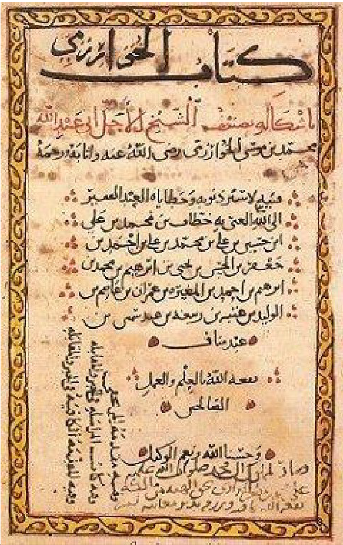
\includegraphics[scale=1]{Sections/FirstDegreeEquationsImages/TextPage.png}	
	\caption{The picture shown above is a page from \quotes{\textit{Al-Kit\={a}b al-mukhta$\stackrel[^\textrm{.}]{}{\textrm{s}}$ar f\={i} $\stackrel[^\textrm{.}]{}{\textrm{h}}$is\={a}b al-jabr wa-l-muq\={a}bala}} written in the early-mid 800’s C.E. by the Persian mathematician Ab\={u} Abdall\={a}h Mu$\stackrel[^\textrm{.}]{}{\textrm{h}}$ammad ibn M\={u}s\={a} al-Khw\={a}rizm\={i}. His work is generally considered to be the first major step toward modern algebra (the word \quotes{algebra} actually comes from the word \quotes{al-jabr} in the title.)  The book’s Arabic title translates into English as 'The Compendious Book on Calculation by Completion and Balancing'.}
\end{SCfigure}

%\footnote{By Al-Khwarizmi - Esposito, John L. , ed. (1999) The Oxford History of Islam, Oxford University Press ISBN: 0195107993. ; April 2006 (upload date) by Spm, Public Domain, https://commons.wikimedia.org/w/index.php?curid=716423}

\quotes{Balancing} is one of the most fundamental principles used in algebra.  The basic idea is this: think of an equation as a balanced scale.  The two sides of the equation are equal, and so if we placed them on an imaginary scale, the scale would balance.  If you change the value of one side of the equation (say by adding or subtracting something to it, or multiplying or dividing it by something) the scale will no longer be in balance.  But you can recover that balance by making the same change to the other side.

This all boils down to the following rule:

\begin{definition}
	\index{Equation!Balance Principle}
	\textbf{\underline{The Balance Principle}}\\
	\bigskip
	You can make any change you like to one side of an equation, as long as you make an equivalent change to the other side.
\end{definition}

In algebra, we exploit this rule all the time. Let’s walk through a very basic example to review how it works, and then we’ll proceed to some more complicated problems.

Suppose we want to solve:
$$25 - 0.03m = 10$$

and let’s also forget that anyone ever said anything about trying any particular values as solutions.  Let’s just suppose we are given the equation and are asked to determine its solution.

So, our goal is to get an equation which directly tells us the correct value of $m$. So, what we will do here is to try to transform the given equation into something that just has the variable $m$ isolated on one side, and a number on the other side.

Let’s begin by getting rid of the $25$. We can eliminate that $25$ on the left by subtracting it - and we are allowed to do that so long as we also subtract $25$ from the right, to keep the equation balanced. So:
\begin{align*}
	25-0.03m\bm{-25} & = 10\bm{-25}\\
	-0.03m & = -15
\end{align*}

Now, we don’t have $m$ isolated yet, but we’re closer. We now just have to get rid of the coefficient $-0.03$. Now, it is a common mistake to try to do this by adding $0.03$ to both sides, but that won’t work because $-0.03m$ and $0.03$ are not like terms, and so they cannot be combined.  But we can divide both sides by $-0.03$:
$$\frac{-0.03m}{\bm{-0.03}} = \frac{-15}{\bm{-0.03}}$$

Which gives us:
$$m = 500$$

So we conclude that the solution is $m = 500$.  Stating this solution in terms appropriate for the question at hand we might phrase it as \quotes{$500$ minutes of usage}. We can also feel confident that this is the only solution, because this is the only solution that we arrived at by following the methods of algebra.

Using the principle of balance to transform an equation into one which explicitly states its solution is one of the primary methods of algebra, and really the only technique we will be using in this chapter. However, with more complicated equations, the strategies to use to get the variable by itself may be more involved. The following examples will illustrate how the principle of balance can be used effectively with some of these more complicated equations.

\exam{\label{FirstDegreeEquationsExample2}Solve for $x$: $$5x-11+3(2x-3)=2$$}

\indenttext{
	Before putting the principle of balance to work on this, it would be best to simplify by distributing
	and combining like terms. So:
	\begin{align*}
		5x-11+3(2x-3)&=2\\
		5x-11+6x-9&=2\\
		11x-20&=2
	\end{align*}

	From here, we just need to add $20$ and then divide by $11$ to get isolate the $x$:
	\begin{align*}
		11x-20&=2\\
		11x&=22\\
		x&=2
	\end{align*}

	It never hurts to check your answers by substituting your solution back into the original equation:
	\begin{align*}
		5x-11+3(2x-3)&=2\\
		5(2)-11+3(2(2)-3)&=2\\
		2&=2
	\end{align*}

	Since the equation holds true when we substitute in $x=2$, the solution checks as correct.
}

Often we run into equations where the variable appears on both sides. In those cases, the best strategy is usually to first simply both sides as much as possible, and then collect all the variable terms together on one side, and all the non-variable terms on the other. The following example will illustrate:

\exam{\label{FirstDegreeEquationsExample3}Solve for $z$: $$5(z+1)-16=3z-5$$}

\indenttext{
	\begin{align*}
		5(z+1)-16&=3z-5\\
		5z+5-16&=3z-5\\
		5z-11&=3z-5
	\end{align*}

	It doesn’t matter which side we collect the $z$’s on; either is fine.  It is more common to collect them on the left, so we’ll subtract $3z$ from both sides to get:
	$$2z-11=-5$$

	Now since we’ve collected $z$’s on the left, we’ll add $11$ to both sides to get rid of the $-11$ on the left:
	$$2z=6$$

	And now dividing both sides by 2 we get:
	$$z=3$$

	A check confirms the result:
	\begin{align*}
		5(z+1)-16&=3z-5\\
		5(3+1)-16&=3(3)-5\\
		4&=4
	\end{align*}
}

Let’s try one more example before moving on.

\exam{\label{FirstDegreeEquationsExample4}Solve for $t$: $$4t-3-7(2-t)=2(7t+5)-(t-4)$$}

\indenttext{
	As before, we’ll simplify each side first. Remember that you need to be careful about the negatives when distributing!
	\begin{align*}
		4t-3-7(2-t)&=2(7t+5)-(t-4)\\
		\\
		4t-3-14+7t&=14t+10-t+4\\
		\\
		11t-17&=13t+14
	\end{align*}

	Now, as mentioned in the previous example, there is a tendency to collect the variable on the left.  So, if we collect the variable on the left we subtract $13t$ from both sides to get:
	$$-2t-17=14$$

	Then add $17$ to both sides:
	$$-2t=31$$

	And now divide by $-2$:
	$$t=\frac{31}{-2}$$ 
	
	which is more commonly rewritten as: 
	$$t=-\frac{31}{2}=\frac{-31}{2}=-15.5$$

	Some people feel a strong preference against negative coefficients if they can be avoided, and so might prefer to subtract $11t$ from both sides. That is also fine, and in fact we can do this and then switch the equation’s sides if we want to. So this is also a correct solution:
	\begin{align*}
		4t-3-7(2-t)&=2(7t+5)-(t-4)\\
		\\
		4t-3-14+7t&=14t+10-t+4\\
		\\
		11t-17&=13t+14\\
		\\
		-17&=2t+14\\
		\\
		-31&=2t\\
		\\
		-\frac{31}{2}&=t
	\end{align*}

	Finally, to check. We’ll substitute this solution into the original equation. Since the arithmetic gets tedious, typing each side’s expression into the calculator is probably the best choice; remember though to be careful to use parentheses appropriately when substituting in this negative number:
	\begin{align*}
		4t-3-7(2-t)&=2(7t+5)-(t-4)\\
		\\
		4\left(\frac{-31}{2}\right)-3-7\left[2-\left(\frac{-31}{2}\right)\right]&=2\left[7\left(\frac{-31}{2}\right)+5\right]-\left[\left(\frac{-31}{2}\right)-4\right]\\
		\\
		-187.5&=-187.5
	\end{align*}
}

As the choice discussed in the above example makes clear, we often have some choice about the order we do things. While the examples given in this book are meant to illustrate sound strategy, all of these problems can be correctly solved in other ways as well. \textbf{As long as the steps you take follow the laws of algebra} you will arrive at a correct solutions.

%%%%%%%%%%%%%%%%%%%%%%%%%%%%%%%%%%%%%%%%%%%%%%%%%%%%%%%%%%%%%%%%%%%%%%
%
% Subsection: First Degree Equations: Solving Equations Involving Fractions
%
%%%%%%%%%%%%%%%%%%%%%%%%%%%%%%%%%%%%%%%%%%%%%%%%%%%%%%%%%%%%%%%%%%%%%%

\subsection{Solving Equations Involving Fractions}

When equations involve fractions, the same principles apply, but the arithmetic can quickly become tedious. Arithmetic with fractions is much more work than arithmetic with whole numbers, even when using a calculator.

We can avoid fraction arithmetic by multiplying both sides of the equation through by a common denominator.  This technique is known as \textbf{clearing the fractions}. The following example will illustrate.

\exam{\label{FirstDegreeEquationsExample5}Solve for $y$: $$\frac{2}{3}y-\frac{7}{5}=\frac{1}{6}y+\frac{11}{4}$$ }

\indenttext{
	Among the denominators $3,5,6,$ and $4$ is 60.  So, to clear the fractions, we start by multiplying both sides by 60.
	\begin{align*}
		60\left(\frac{2}{3}y-\frac{7}{5}\right)&=60\left(\frac{1}{6}y+\frac{11}{4}\right) \\
		\\
		60\left(\frac{2}{3}y\right)-60\left(\frac{7}{5}\right)&=60\left(\frac{1}{6}y\right)+60\left(\frac{11}{4}\right)\\
		\\
		\frac{120}{3}y-\frac{420}{5}&=\frac{60}{6}y+\frac{660}{4}\\
		\\
		40y-84&=10y+165
	\end{align*}

	Now, notice what happened when we multiplied; because all of the denominators divide 60 evenly, the result in each term is a whole number.  Now we can just continue as we have before:
	\begin{align*}
		40y-84&=10y+165 \\
		\\
		30y-84&=165 \\
		\\
		30y&=249 \\
		\\
		y&=\frac{249}{30}=\frac{83}{10}=8.3
	\end{align*}

	The reduction of the fraction to lowest terms is useful for expressing the exact answer to the equation.  This answer can be checked by substituting back into the original equation (use your calculator for the arithmetic!)
}

It is not absolutely necessary to use the lowest common denominator to clear the fractions from an equation; any common denominator will work. So in the previous example, we could also have just multiplied all the denominators together to get a common denominator and so multiplied both sides by $(3)(5)(6)(4) = 360$. This would have worked out just fine, though the numbers we would have gotten would have been larger after clearing. The benefit of using the lowest common denominator is that it keeps the numbers as small as possible. That is nice, but not mandatory.

Be careful when clearing the fractions if the original equation contains parentheses. When fractions fall inside parentheses, sometimes you may need to multiply through by a common denominator more than once to fully clear all the fractions. The following two examples will illustrate this.

\exam{\label{FirstDegreeEquationsExample6}Solve for $x$: $$\frac{2}{3}x-1=\frac{3}{5}\left(\frac{1}{2}x+1\right)$$}

\indenttext{
	Here the lowest common denominator is $30$, so we multiply both sides:
	$$30\left(\frac{2}{3}x-1\right)=30\left[\frac{3}{5}\left(\frac{1}{2}x+1\right)\right]$$

	When simplifying we generally work from inside parentheses out, but here we are better off multiplying
	30 into the outermost parenthesis on the right first:
	$$30\left(\frac{2}{3}x-1\right)=18\left(\frac{1}{2}x+1\right)$$

	Now continuing as we have before:
	\begin{align*}
		20x-30&=9x+18\\
		\\
		11x-30&=18\\
		\\
		11x&=48\\
		\\
		x&=\frac{48}{11}=4.3636...
	\end{align*}
}

\exam{\label{FirstDegreeEquationsExample7}Solve for $t$: $$\frac{1}{4}\left(\frac{3}{8}t+1\right)=\frac{2}{3}t-1$$}

\indenttext{
	Here the lowest common denominator is $24$, so we multiply both sides:
	\begin{align*}
		24\left[\frac{1}{4}\left(\frac{3}{8}t+1\right)\right]&=24\left(\frac{2}{3}t-1\right)\\
		\\
		6\left(\frac{3}{8}t+1\right)&=24\left(\frac{2}{3}t-1\right)\\
		\\
		\frac{9}{4}t+6&=16t-24	
	\end{align*}

	Now the fractions turn out to no be fully cleared out.  So, we have to multiply a second time, this time by $4$ to get:
	\begin{align*}
		4\left(\frac{9}{4}t+6\right)&=4\left(16t-24\right)\\	
		\\
		9t+24&=64t-96
	\end{align*}

	Now, with the fractions cleared, we proceed:
	\begin{align*}
		9t+24&=64t-96\\
		\\
		120&=55t\\
		\\
		t&=\frac{120}{55}=\frac{24}{11}=2.1818...
	\end{align*}
}

Clearing the fractions is optional. All of the above examples can be done without it, just working through the algebra with fraction arithmetic. Most people find it easier to clear the fractions instead, but this is a matter of choice not necessity. The choice is yours.

%%%%%%%%%%%%%%%%%%%%%%%%%%%%%%%%%%%%%%%%%%%%%%%%%%%%%%%%%%%%%%%%%%%%%%
%
% Subsection: First Degree Equations: Identities and Contradictions
%
%%%%%%%%%%%%%%%%%%%%%%%%%%%%%%%%%%%%%%%%%%%%%%%%%%%%%%%%%%%%%%%%%%%%%%

\subsection{Identities and Contradictions}

Not all problems can be solved! This fact of life shows up with equations as well. Suppose you are asked to find a solution for the equation:

$$ x = x + 1 $$

Without even trying any algebra on it, we can see we have a problem. The equation says that $x$ must be equal to $x+1$. Any solution to this equation would have to be equal to itself plus one! That’s impossible – no number is one bigger than itself. So there is no way that this equation could ever have a solution. Equations like this one that have no solutions are called \textbf{inconsistent} \index{Equation!Inconsistent} or \textbf{contradictions} \index{Equation!Contradiction}.

Now, not all inconsistent equations are as transparent as this one. For example, the equation:
$$5(x-2)+3(x+1)=2x+1-3(11-2x)$$

is also inconsistent. But while it is pretty obvious that no number can equal itself plus one, it is not even remotely obvious that it is impossible for five times a two less than a number plus three times one more than that number to equal one more than twice the number less three times eleven take away twice the number! So, how can we tell if an equation is inconsistent?

Let’s see what would happen if we tried to use algebra to solve this equation:
\begin{align*}
	5(x-2)+3(x+1)&=2x+1-3(11-2x)\\
	\\
	5x-10+3x+3&=2x+1-33+6x\\
	\\
	8x-7&=8x-32\\
	\\
	-7&=-32
\end{align*}

When we try to get the $x$'s on one side by subtracting $8x$ from both sides and get an equality which is nonsense as $-7$ is not equal to $-32$.  And \underline{that} is what tells us that this equation is inconsistent. We followed the methods of algebra in good faith, assuming that there was a solution, and those methods led us to the absurd conclusion. So, if you believe this equation has a solution, you then also have to believe that $-7=-32$!  Unless you are willing to allow this as true, you have to conclude that the equation has no solution.

The solution set of an inconsistent equation is an empty set. Since there are no solutions, the set has no members. This set is commonly called the \textbf{empty set} or the \textbf{null set} and is represented with the symbol $\emptyset$. Be careful not to confuse the empty set with the number $0$. They look similar, but they are not at all the same thing. It is correct to say that this equation’s solution set is $\emptyset$, but it is completely wrong to say that the solution set is $0$ or to say that $0$ is a solution to the equation.

On the other hand, sometimes an equation has lots and lots of solutions. For example, consider the equation:
$$6x+10=2(3x+5)$$

It’s probably not immediately obvious that this is not an ordinary equation, but think about what would happen if you distributed the $2$ into the parentheses on the right. You’d wind up with the equation:
$$6x+10=6x+10$$

Now, this is true no matter what you substitute in for $x$! Any real number is a solution for it. Equations like this are called \textbf{identities} \index{Equation!Identity}. Because any real number satisfies an identity, we say that its solution set is the set of all real numbers, which we often indicate using the symbol $\mathbb{R}$.

Just as many inconsistent equations are not obviously so, many identities are not obvious identities. For example, this equation is an identity:
$$4x-2(3x-5)=7x-3(3x-3)+1$$

but that’s not obvious at all. How can we tell?

Well, suppose we set out to solve this equation:
\begin{align*}
	4x-2(3x-5)&=7x-3(3x-3)+1\\
	\\
	4x-6x+10&=7x-9x+9+1\\
	\\
	-2x+10&=-2x+10
\end{align*}

Now, at this point we have the same expression on both sides of the equation, which is a dead giveaway.  If the two sides are the same, then they will be equal irrespective of what $x$ might be. If, though, you don’t notice that they are the same, you could continue and add $2x$ to both sides and get:
$$10=10$$

No matter what $x$ is, $10$ is equal to itself. So, this also tells us that we have an identity on our hands!

(Be careful here! It is a common mistake to misread this last equation as saying that the solution is $10$. This last equation does not say that $x=10$, it says that $10=10$. That is true no matter what $x$ is, which is why we conclude that this is an identity.)

When given an equation to solve, it is always a possibility that the equation may turn out to be an inconsistent equation or an identity. But if it is, that will become apparent as you work to solve it.  If it is inconsistent, that will become apparent once the algebra leads you to an absurd equation; if it is inconsistent that will become apparent once the algebra leads you to an equation whose sides are both the same. If it is an ordinary equation with a solution (called a \textbf{conditional equation} \index{Equation!Conditional}) the algebra will take you there, too.

\exam{\label{FirstDegreeEquationsExample8}Solve for $P$: $$3P-5(4P-3)=-3(5P-1)-2P$$}

\indenttext{
	\begin{align*}
		3P-5(4P-3)&=-3(5P-1)-2P\\
		\\
		3P-20P+15&=-15P+3-2P\\
		\\
		-17P+15&=-17P+3\\
	\end{align*}

	At this point you may notice that we have an impossible situation in the equation, but it does no harm to continue. Adding $17P$ to both sides we get:
	$$15=3$$

	which is clearly impossible, no matter what value we might substitute in for $P$. The equation is a contradiction; its solution set is $\emptyset$.
}

%%%%%%%%%%%%%%%%%%%%%%%%%%%%%%%%%%%%%%%%%%%%%%%%%%%%%%%%%%%%%%%%%%%%%%
%
% Subsection: First Degree Equations: Solve for variable
%
%%%%%%%%%%%%%%%%%%%%%%%%%%%%%%%%%%%%%%%%%%%%%%%%%%%%%%%%%%%%%%%%%%%%%%

\subsection{Solving for One Variable in Terms of Others}

In Section \ref{AlgebraicSubstitution} we used the formula:
$$W=210-\frac{m}{3}$$

which expresses the relationship between $m$, minutes of vigorous exercise per day, and $W$, a given person’s projected weight after one year. In the examples of that section, we substituted in values of $m$ and found the resulting values of $W$.

This works great if you know the minutes of exercise and want to know the projected weight, but what if the situation is reversed? Suppose we have in mind a desired weight and want to know the minutes of exercise that would be needed to achieve that. For example, suppose we want to know the minutes of exercise needed to achieve a weight of $185$ pounds? Well, we could substitute in $W=185$ to get the equation:
$$185=210-\frac{m}{3}$$

which we could then solve for $m$:
\begin{align*}
	185&=210-\frac{m}{3} \\
	\\
	3(185) &= 3 \left(210 - \frac{m}{3}\right) \\
	\\
	555 &= 630 - m \\
	\\
	-75 &= -m \\
	\\
	m &= 75
\end{align*}

So, $185=210-\frac{m}{3}$ implies that $75$ minutes of daily exercise would be required.

Now, that’s fine if we only need to find the minutes required for one weight, but what if we want to be able to find the minutes required for several different weights? It would be tedious to have to work through essentially the same algebra over and over again. Instead, why not rework the original equation so that it is set up to plug in $W$ and give $m$ as a result. We call this solving for $m$ in terms of $W$.

The algebra principles and methods we use are essentially the same as we’ve been using, except that instead of getting a number as a solution, we expect the result to be a formula:
\begin{align*}
	W&=210-\frac{m}{3} \\
	\\
	3W &= 3 \left(210 - \frac{m}{3}\right) \\
	\\
	3W &= 630 - m \\
	\\
	3W-630 &= -m \\
	\\
	(-1)(3w-630)&=(-1)(-m)\\
	\\
	-3W+630&=m
\end{align*}

which we can now rewrite as:
$$m=-3W+630 \text{ or } m=630-3W$$

It should be apparent that this new equation is set up to give values of $m$ readily once a value of $W$ is plugged in.

\exam{\label{FirstDegreeEquationsExample9}The equation $C=\frac{5}{9}(F-32)$ gives $C$, the temperature in degrees Celsius, in terms of $F$, the temperature in degrees Fahrenheit. Solve this equation for $F$ in terms of $C$.}

\indenttext{
	\begin{align*}
		C&=\frac{5}{9}(F-32)\\
		\\
		9C&=9\left(\frac{5}{9}(F-32)\right)\\
		\\
		9C&=5(F-32)\\
		\\
		9C&=5F-160\\
		\\
		9C+160&=5F\\
		\\
		\frac{9C+160}{5}&=F
	\end{align*}

	which we can then rewrite as:
	$$F=\frac{9C+160}{5}$$

	This is a correct solution. It would also be fine to divide the $5$ into each term, giving a final answer of $F=\frac{9}{5}C+32$ or to rewrite the division by $5$ as multiplication by $\frac{1}{5}$, giving a final answer of $F=\frac{1}{5}\left(9C+160\right)$.
}

Most of the time in this course our equations will involve at most two variables, but there is no reason we can’t do this with equations involving more variables.

\exam{\label{FirstDegreeEquationsExample10} Solve for $L$ in terms of the other variables in $P=2L+2W$}

\indenttext{
	\begin{align*}
		P&=2L+2W\\
		\\
		P-2W&=2L\\
		\\
		\frac{P-2W}{2}&=L\\
	\end{align*}

	$$L=\frac{P-2W}{2} \text{ or } L=\frac{1}{2}\left(P-2W\right)$$
}

%%%%%%%%%%%%%%%%%%%%%%%%%%%%%%%%%%%%%%%%%%%%%%%%%%%%%%%%%%%%%%%%%%%%%%
%
% Subsection: First Degree Equations: Exercises
%
%%%%%%%%%%%%%%%%%%%%%%%%%%%%%%%%%%%%%%%%%%%%%%%%%%%%%%%%%%%%%%%%%%%%%%

\clearpage

\subsection{Exercises}

\subsubsection*{Solutions to Equations}
Determine which, if any, of the given values satisfy the given equations.

\ex{$3x-7=8$; \indent $x=1,2,3,4,\text{ or }5$} \sol{$x=5$} 
\bigskip

\ex{$14-3x=20$; \indent $x=-3,-2,-1,0,1,2,\text{ or }3$}
\bigskip

\ex{$x^2-2x=0$; \indent $x=-2,-1,0,1,\text{ or }2$} \sol{$x=0$ and $x=2$}
\bigskip

\ex{$5-y^2=1$; \indent $y=-2,-1,0,1,\text{ or }2$}
\bigskip

Answer each of the following questions based on the information given. Justify your answers.\\

\ex{A technology sales rep quotes the costs for backup data storage systems using the formula $C=50+0.12d$ where $d$ is the number of gigabytes of storage used.  I asked the sales rep to quote me costs for $1000,2000,3000,5000,$ and $10,000$ gigabytes. She wrote up a quote showing a cost of $650$, but the quote doesn’t show the amount of storage that’s based on, and I can’t remember what she used to determine the quote. What amount of storage is the quote based on?
} 
\sol{$5000$ gigabytes}
\bigskip

\ex{My water bill $W$ is calculated using the formula $W=0.02g+5$ where $g$ is the number of gallons used during the month. Last month my bill was $\$25$, but I’m not sure whether I used $500, 1000, 1500,$ or $2000$ gallons. Which of these possibilities, if any, was my actual usage?}
\bigskip

\ex{The mass of carbon dioxide $m$ in grams in a pressurized tank at room temperature is given by the formula $m=44x$ where $x$ is the volume of the tank in liters. A supplier can provide pressurized tanks with volumes of $5,10,20,$ or $50$ liters.  A chemist wrote down that he needed to order a tank with $176$ grams of carbon dioxide, but didn’t write down the volume tank this was based on. What size tank does he need to order?} \sol{20 liters}
\bigskip

\ex{A landscaper estimates that the time required to cut the grass in an athletic field, $h$ (in hours) based on the size of the field, $A$, in square yards is given by the formula $h=\frac{A}{800}+1$. The town has five athletic fields, measuring $1200, 2000, 2800, 3200,$ and $4800$ square yards. He scheduled one of his workers for four and one half hours to cut the grass on one of the town’s fields, but forgot to say which field it was. Which field is she supposed to cut?}
\bigskip

\subsubsection*{Solving Equations Using the Balance Principle}

Solve each of the following equations. If your final answer is a fraction, reduce it to lowest terms.
\begin{tasks}[label={}](2)
	\task\ex{$3x-23=37$} \sol{$x=20$}
	\task\ex{$5x-47=103$}
	\task\ex{$2x+7=32$} \sol{$x=\frac{25}{2}=12.5$}
	\task\ex{$6x+1=13$}
	\task\ex{$9-2z=11$} \sol{$z=-1$}
	\task\ex{$6-5z=36$}
	\task\ex{$3x+2=11+2x$} \sol{$x=9$}
	\task\ex{$7x-3=5x+11$}
	\task\ex{$5x-13=8x+20$} \sol{$x=-11$}
	\task\ex{$7x+2=3x-18$}
	\task\ex{$21x+13=9x-20$} \sol{$x=\frac{-11}{4}=-2.75$}
	\task\ex{$15x-5=61-x$}
	\task\ex{$3(y-2)+2y=14$} \sol{$y=4$}
	\task\ex{$2(y+5)+3y=25$}
	\task\ex{$4(d-1)+3(5-d)=0$} \sol{$d=-11$}
	\task\ex{$6(k+5)-(10+k)=20$}
	\task\ex{$3x+2(3x-5)=7x-4$} \sol{$x=3$}
	\task\ex{$4(2x-1)-2(3x-5)=12$}
\end{tasks}

\bigskip
\ex{$5(3x-1)-2(7x+1)=3(2x+5)-(x+1)$} \sol{$x=\frac{-21}{4}=-5.25$}

\bigskip
\ex{$5t-3(t+1)=4(2t+1)+5$}

\bigskip
\ex{$4h-5(2h-6)=3(h-5)+2(h+3)$}  \sol{$h=\frac{39}{11}=3.5454...$}

\bigskip
\ex{$6(2t-3)-5(3t+1)=3(2t+1)+7(t-3)$}

\bigskip
\ex{A technology sales rep quotes the costs for backup data storage systems using the formula$C=50+0.12d$ where$ d$ is the number of gigabytes of storage used. She wrote up a quote showing a cost of $\$1850$, but the quote doesn’t show the amount of storage that’s based on, and I can’t remember what she used to determine the quote. What amount of storage is the quote based on?}  \sol{$15,000$ gigabytes}

\bigskip
\ex{My water bill$ W$ is calculated using the formula $W=0.02g+5$ where $g$ is the number of gallons used during the month. Last month my bill was $\$37.68$, but I’m not sure how much water I used. How many gallons did I use last month?}

\bigskip
\ex{The mass of carbon dioxide $m$ in grams in a pressurized tank at room temperature is given by the formula $m=44x$ where$x$ is the volume of the tank in liters. A chemist wrote down that he needed to order a tank with $880$ grams of carbon dioxide, but didn’t write down the volume tank this was based on. What size tank does he need to order?} \sol{$20$ liters}

\bigskip
\ex{A landscaper estimates that the time required to cut the grass in an athletic field, $h$ (in hours) based on the size of the field, $A$, in square yards is given by the formula $h=\frac{A}{800}+1$. He scheduled one of his workers for five hours to cut the grass on one of the town’s fields. How many square yards does the field measure?}

\bigskip

\subsubsection*{Solving Equations Involving Fractions}
Solve each of the following equations. If your final answer is a fraction, reduce it to lowest terms.
\begin{tasks}[label={}](2)
	\task\ex{$\frac{1}{3}x-1=\frac{5}{2}$}  \sol{$\frac{21}{2}=10.5$}
	\task\ex{$\frac{1}{4}x-3=\frac{2}{5}$}
	\task\ex{$\frac{3}{8}x+\frac{5}{2}=\frac{5}{6}x-\frac{1}{3}$} \sol{$x=\frac{68}{11}=6.1818...$}
	\task\ex{$\frac{2}{5}x+\frac{9}{10}=\frac{1}{2}x-\frac{3}{4}$}
	\task\ex{$\frac{3}{2}p-1=\frac{5}{8}p-3$} \sol{$p=\frac-{16}{7}$}
	\task\ex{$\frac{2}{3}r+5=\frac{1}{9}r+25$}
	\task\ex{$\frac{y-2}{3}=\frac{y+5}{2}$} \sol{$y=-19$}
	\task\ex{$\frac{x+2}{5}=\frac{x-1}{3}$}
	\task\ex{$\frac{2x-1}{5}+3=\frac{3x}{10}$} \sol{$x=-28$}
	\task\ex{$\frac{4x+3}{20}x=1+\frac{x-1}{5}$}
	\task\ex{$\frac{1}{2}\left(\frac{3}{5}z-\frac{1}{4}\right)=3$} \sol{$z=\frac{125}{12}=10.4166...$}
	\task\ex{$\frac{2}{7}\left(\frac{1}{2}y+\frac{3}{14}\right)=\frac{3}{7}y-1$}

\end{tasks}

\subsubsection*{Identities and Contradictions}

Each of the following equations is either an identity or a contradiction (inconsistent equation).  Determine which.  Justify your answer.

\ex{$3(2x-5)=2(3x-7)$}  \sol{contradiction or inconsistent}

\bigskip
\ex{$5(3x-1)=3(5x+1)$}

\bigskip
\ex{$4x-3(x+5)=7(x+2)-3(2x+1)$} \sol{contradiction or inconsistent}

\bigskip
\ex{$8x-3(2x+1)=5x-3(x+1)$}

\bigskip
\ex{$6x-24=3(2x-8)$} \sol{Identity}

\bigskip
\ex{$6(2x-5)=2(6x-15)$}

\bigskip
\ex{$5(x+2)-(4x-1)=7(x-2)-3(2x-1)$} \sol{contradiction or inconsistent}

\bigskip
\ex{$8(2x-5)-2(3x+1)=3(3x+1)-(7-x)$}

\bigskip

\subsubsection*{Solving for One Variable in Terms of Others}

Solve each of the following equations for the requested variable in terms of the other variable(s).

\begin{tasks}[label={}](2)
	\task\ex{$y=2x-10$ for $x$} \sol{$x=\frac{y+10}{2}$}
	\task\ex{$y=5-3x$ for $x$}
	\task\ex{$P=10+2W$ for $W$} \sol{$\frac{P-10}{2}$}
	\task\ex{$v=80-16t$ for $t$}
	\task\ex{$z=\frac{x-100}{15}$ for $x$} \sol{$x=15z+100$}
	\task\ex{$z=\frac{x-60}{12}$ for $x$}
	\task\ex{$F=\frac{9}{5}K-460$ for $K$} \sol{$K=\frac{5}{9}\left(F+460\right)$}
	\task\ex{$m=\frac{3}{5}t-1$ for $t$}
	\task\ex{$I=PRT$ for $P$} \sol{$P=\frac{I}{RT}$}
	\task\ex{$I=PRT$ for $R$}
	\task\ex{$z=\frac{x-\mu}{\sigma}$ for $x$}  \sol{$x=\mu+z\sigma$}
	\task\ex{$z=\frac{x-\mu}{\sigma}$ for $\mu$}
	\task\ex{$z=\frac{x-\mu}{\sigma}$ for $\sigma$} \sol{$\sigma=\frac{x-\mu}{z}$}
	\task\ex{$E=mc^2$for$m$}
\end{tasks}

\bigskip
\ex{The mass of carbon dioxide $m$ in grams in a pressurized tank at room temperature is given by the formula $m=\frac{44x}{5}$ where $x$ is the volume of the tank in liters. This formula is set up to give the mass based on the volume. A chemist needs a formula which is instead set up to give the volume based on the mass.  Solve the equation for $x$ in terms of $m$ to create the desired formula.}  \sol{$x=\frac{5}{44}m$}

\bigskip
\ex{A landscaper estimates that the time required to cut the grass in an athletic field, $h$ (in hours) based on the size of the field, $A$, in square yards is given by the formula $h=\frac{h}{800}+1$. He wants a formula which gives the size of the field based on the time it takes to mow it.  Solve the equation for $A$ in terms of $h$ to create the formula he wants.}

\bigskip

\subsubsection*{General Exercises}

\ex{Solve $3x-2=5x-8$} \sol{$x=3$}

\bigskip
\ex{Solve $4(5x-1)+3=10(2x+3)$}

\bigskip
\ex{Solve for $z$: $x=3z+2y-5$}  \sol{$z=\frac{x-2y+5}{3}$}

\bigskip
\ex{Solve $5y-1=3y+1$}

\bigskip
\ex{Solve $4(x+2)-3(x+1)=x+5$}  \sol{Identity}

\bigskip
\ex{What is the solution set of the equation $3x+5(x-3)=1$?}

\bigskip
\ex{What is the solution set of the equation $4(2x-5)=8(x-1)$?} \sol{$\emptyset$}

\bigskip
\ex{The daily profit for a tour operator $p$ depends on the number of paying customers taking his tour $t$. The relationship is expressed by the equation $p=65t-350$. Yesterday he made a profit of $\$820$. How many paying customers did he have that day?}

\bigskip
\ex{The daily profit for a tour operator $p$ depends on the number of paying customers taking his tour $t$. The relationship is expressed by the equation $p=65t-350$. This equation is set up to most easily give profit based on the number of paying customers. The tour operator would like to have a formula which is set up to give the number of customers needed based on the amount of profit, so that he can easily figure out how many customers he needs to draw to reach his profit goals. Find such a formula, by solving for $t$ in terms of $p$.} \sol{$t=\frac{t+350}{65}$}

\bigskip
\ex{Solve $4x-3(x-2)=6$}

\bigskip
\ex{Solve $5-2x=9+2x$} \sol{$x=-1$}

\bigskip
\ex{Which, if any, of the values $-2$, $-1$, $0$, $1$, $2$ satisfy the equation $x^2+3x+4=2$?}

\bigskip
\ex{Solve $7=2(1-\frac{1}{8}t)$} \sol{$t=-20$}

\bigskip
\ex{Solve $5x+9=2x-12$}

\bigskip
\ex{Solve $3(2x+5)+4(3+x)=2(4x-1)+2x$} \sol{contradiction or inconsistent}

\bigskip
\ex{Solve for $t$: $m=3t-k$}

\bigskip
\ex{Solve $2z-1=5-\frac{1}{3}z$} \sol{$z=\frac{18}{7}$}

\bigskip
\ex{Solve $12x+10=3x+1+3(3x+3)$}

\bigskip
\ex{What is the solution set of the equation $5(2t-3)+1=2(4t+1)$?}  \sol{$\{8\}$}

\bigskip
\ex{What is the solution set of the equation $3x+9=3(x+3)$?}

\bigskip
\ex{The cost of mobile phone service for the month depends on the number of minutes used. The cost $C$ in dollars, including tax, based on $m$ minutes of usage, is given by the formula $C=1.08(4.95+0.05m)$. If my bill for the month is $\$67.99$ how many minutes did I use?} \sol{$1160$ minutes}

\bigskip
\ex{The cost of mobile phone service for the month depends on the number of minutes used. The cost $C$ in dollars, including tax, based on $m$ minutes of usage, is given by the formula $C=1.08(4.95+0.05m)$. This formula is set up to most easily give the cost based on the number of minutes used. In order to manage my phone use to stay within my budget, I’d like to have a formula which is set up to tell me the number of minutes based on the amount I want my bill to be. Find such a formula, by solving for $m$ in terms of $C$.}

\bigskip
\ex{Solve $6y+3(y+4)=y+12$}  \sol{$y=0$}

\bigskip
\ex{Solve $5(3-x)+20=5x+10$}

\bigskip
\ex{Which, if any, of the values $0$, $1$, $2$, $3$, $4$, $5$ satisfy the equation $x^2-4x= 0$?} \sol{$x=0$ and $x=4$}

\bigskip
\ex{Solve for $c$: $E = \frac{1}{2}c^2$}

\bigskip

\clearpage

%%%%%%%%%%%%%%%%%%%%%%%%%%%%%%%%%%%%%%%%%%%%%%%%%%%%%%%%%%%%%%%%%%%%%%
%%%%%%%%%%%%%%%%%%%%%%%%%%%%%%%%%%%%%%%%%%%%%%%%%%%%%%%%%%%%%%%%%%%%%%
%
% Section: Solving Second Degree Equations
%
%%%%%%%%%%%%%%%%%%%%%%%%%%%%%%%%%%%%%%%%%%%%%%%%%%%%%%%%%%%%%%%%%%%%%%

\section{Solving Second Degree Equations}
\label{SolveSecondDegree}

%%%%%%%%%%%%%%%%%%%%%%%%%%%%%%%%%%%%%%%%%%%%%%%%%%%%%%%%%%%%%%%%%%%%%%
%
% Subsection: Solving Second Degree Equations: The Square Root Property
%
%%%%%%%%%%%%%%%%%%%%%%%%%%%%%%%%%%%%%%%%%%%%%%%%%%%%%%%%%%%%%%%%%%%%%%

\subsection{The Square Root Property}

In order to solve a second-degree equation, or an equation with an $x^2$ term, we have to get rid of the exponent to be able to solve for $x$. In many second-degree equations, we can do this simply by taking the square root of both sides of the equation.  For example, to solve the following:
$$x^2=25$$

We could undo the squaring of $x$ by taking the square root of both sides.  There is, though, a wrinkle in this approach.  There are actually two solutions to this equation: $x$ could be $5$ since $5^2=25$, but $x$ could also be $-5$ because $(-5)^2=25$ as well.  The square root function, which is usually denoted using the radical symbol \quotes{$\sqrt{\phantom{a}}$}, is interpreted to mean just the positive square root.  Yet the positive square root is not the only solution to the equation, and so we need to make sure we don't loose the other solution in the algebra.  To do this we follow the \textbf{square root property} \index{Square Root Property} which tells us that we can take the square root of both sides of the equation so long as we acknowledge that there are two possible square roots, the positive and the negative.  We usually do this using the symbol \quotes{$\pm$} which is read as \quotes{plus or minus}.  So the next step in solving $x^2=25$ would be:
$$x=\pm \sqrt{25}$$

leading to the solutions:
$$x=\pm 5$$

It is important to understand that this notation is actually telling us that there are two solutions to the equation.  There is no such number as $\pm 5$.  This notation is just a compact way of expressing that there are to the equation $x^2=25$, specifically it is compact notation for the expression:
$$x=5 \text{ or } x=-5$$

This method can be applied to other equations, as the following example will illustrate:

\exam{\label{SolveSecondDegreeExample1} Solve $4x^2-25=11$}

\indenttext{To apply the square root property we need to solve for $x^2$ as if it were simply a variable.  Thus, we start by adding $25$ to both sides of the equation to obtain:
$$4x^2=36$$

and then we divide both sides by $4$ so that:
$$x^2=9.$$

Applying the square root property now gives:
$$x=\pm \sqrt{9}$$
$$x=\pm 3$$
} 

\exam{\label{SolveSecondDegreeExample2} Solve $2x^2+7=39$}

\indenttext{We start by subtracting $7$ from both sides:
$$2x^2=32$$

To get $x^2$ by itself, we divide by $2$:
$$x^2=16$$

Applying the square root property now gives:
$$x=\pm \sqrt{16}$$
$$x=\pm 4$$
} 

\exam{\label{SolveSecondDegreeExample3} Solve $3z^2-9=z^2+6$}

\indenttext{To do this we first use ordinary algebra to solve for $z^2$, so subtract $z^2$ from both sides:
$$2z^2-9=6$$

and then add $9$ to both sides:
$$2z^2=15$$

Now to get $z^2$ by itself we divide by 2:
$$z^2=\frac{15}{2}$$

Now we are ready to use the square root property.  Doing so we end up with two solutions
$$z=\pm \sqrt{\frac{15}{2}}$$

Since neither $15$ nor $2$ is a perfect square we are stuck on simplifying this any further.  This is a perfectly fine way to express the answer.  If, however, you would like to have a decimal approximation. it can be obtained using your calculator as $z=\pm 2.7386...$.  The problem with converting to a decimal is that it does typically require rounding so it is often preferable to leave your answer in radical notation as that is the exact answer and can be rounded to any level of precision later on.
}

%%%%%%%%%%%%%%%%%%%%%%%%%%%%%%%%%%%%%%%%%%%%%%%%%%%%%%%%%%%%%%%%%%%%%%
%
% Subsection: Solving Second Degree Equations: Factor to Solve
%
%%%%%%%%%%%%%%%%%%%%%%%%%%%%%%%%%%%%%%%%%%%%%%%%%%%%%%%%%%%%%%%%%%%%%%

\subsection{Factor to Solve a Second-Degree Equation}

In some cases, a second degree equation may be written in a way that makes the solutions very easy to find. For example:
$$(x-4)(x+1)=0$$

We know that can be simplified by using the distributive property so we know this is indeed a second degree equation.

We know from basic arithmetic that if you multiply two numbers together and get zero, one of these numbers must be zero.  Formally, this fact is called the \textbf{zero product property}.

%%%%%%%%%%%%%%%%%%%%%%%%%%%%%%%%%%%%%%%%%%%%%%%%%%%%%%%%%%%%%%%%%%%%%%
%
% Definition: Zero Product Principle
%
%%%%%%%%%%%%%%%%%%%%%%%%%%%%%%%%%%%%%%%%%%%%%%%%%%%%%%%%%%%%%%%%%%%%%%

\begin{definition}
	\index{Zero Product Principle}
	\textbf{\underline{Zero Product Principle}}\\
	\bigskip
	If $AB=0$, then either $A=0$ or $B=0$.
\end{definition}

Now, in this equation we have two expressions being multiplied together: $x-4$ and $x+1$.  The equation says that their product is zero.  So, according to the zero product property, the only possibilities are
$$x-4=0 \text{ or } x+1=0$$

Using this fact we know there are two possibilities to consider. One is that $x-4=0$. If that is the case, then we can easily solve and see that $x=4$. The other possibility is that $x+1=0$. In that case, we can also easily solve and see that $x=-1$. So, we conclude that this equation’s solutions are $x=4$ and $x=-1$.  When a second degree equation is written in a form like this, as a product, we can find the solutions simply by setting each of the factors equal to zero and solving. Here is another example:

\exam{\label{SolveSecondDegreeExample4} Solve: $5(2x-3)(x+7)=0$}

\indenttext{To solve $5(2x-3)(x+7)=0$ we set each factor equal to zero and determine if that leads to a consistent equation.  Since the product is zero, we can apply the zero product principle to conclude that either $5=0$ or $2x-3=0$ or $x+7=0$.  Since the first factor is a number and it is not equal to zero, we get a contradiction as $5 \ne 0$.  Thus, the first factor does not lead to a solution to the equation in question.  The second factor, $2x-3$ is zero when $x=\frac{3}{2}$.  The third factor $x+7$ is zero when $x=-7$.  Thus, there are two solutions to the equation $x=\frac{3}{2}$ and $x=-7$.
}

As we saw in section \ref{SecondDegreeFactor} this second-degree equation is written as the product of expressions, or we can say in factored form.  In some cases, we can use the method given to us in section \ref{SecondDegreeFactor} to factor the second degree expression to help us solve. To review:

%%%%%%%%%%%%%%%%%%%%%%%%%%%%%%%%%%%%%%%%%%%%%%%%%%%%%%%%%%%%%%%%%%%%%%
%
% Definition: Factor Second Degree Expression
%
%%%%%%%%%%%%%%%%%%%%%%%%%%%%%%%%%%%%%%%%%%%%%%%%%%%%%%%%%%%%%%%%%%%%%%

\begin{definition}
	\textbf{\underline{Factoring Second Degree Expressions of the Form $x^2+bx+c$}}\\
	\bigskip
	\begin{enumerate}
		\item[$\cdot$] Consider all the pairs of integers whose product is $c$
		\item[$\cdot$] If the sum of any of the pairs is $b$, then the expression can be factored to $(x+m)(x+n)$ where $m$ and $n$ are the integers.
		\item[$\cdot$] If none of the pairs sum to $b$, then the expression cannot be factored using integers. We then say is it \quotes{not factorable over the integers}.
	\end{enumerate}

	When groupings of the same variable raised to power or exponents, you can just add the exponents\\ (make sure to remember that a ‘plain’ $x$ is actually $x^1$).
	$$x^a \cdot x^b = x^{a+b}$$
\end{definition}

\exam{\label{SolveSecondDegreeExample5} Factor $x^2-5x+6$}

\indenttext{We need to consider all possible pairs of integers whose product is $6$ and then look at their sum to see if it is possible to obtain a sum of the factors equal to $-5$.  We consider all possible pairs $1$ and $6$ (sum $7$), $-1$ and $-6$ (sum $-7$), $2$ and $3$ (sum $5$), and $-2$ and $-3$ (sum $-5$).  The last pair of factors are the factors that we want and $x^2-5x+6=(x-2)(x-3)$
}

In this case, there were not many possibilities to consider, and one of those possibilities worked. In many cases, though, there are either too many possible pairs to consider, or the expression can’t be factored over the integers at all.  In the special case where the expression can be readily factored, solving by factoring is a reasonable method to use.

\exam{\label{SolveSecondDegreeExample6} Solve $x^2-5x+6=0$ using factoring}

\indenttext{Using example \ref{SolveSecondDegreeExample5}, we can factor the left side of the equation as $(x-2)(x-3)=0$.  Applying the zero product principle we see that the solutions to the equation come from $x-2=0$ or $x-3=0$.  Thus, the solutions we are looking for are $x=2$ and $x=3$.}

\exam{\label{SolveSecondDegreeExample7} Solve $x^2+8x+7=0$ using factoring}

\indenttext{There are not too many possibilities to consider here, since $7$ is prime, and so the only pairs to consider are $7$ and $1$ or $-7$ and $-1$. Since $7 + 1 = 8$ we can factor this expression in $(x+1)(x+7)$ so we need to consider:
$$(x+1)(x+7)=0$$

Setting each factor equal to zero, we solve $(x+1)(x+7)=0$. So either $x+1=0$ in which case $x=-1$ or $x+7=0$ in which case $x=-7$. So the solutions are $x=-1$ and $x=-7$.
}

\exam{\label{SolveSecondDegreeExample8} Solve $x^2-9x+20=0$ using factoring}

\indenttext{We consider the possibilities that factors of $20$ which are $4$ and $5$ (sum $9$), $-4$ and $-5$ (sum $-9$), $10$ and $2$ (sum $12$), $-10$ and $-2$ (sum $-12$), $20$ and $1$ (sum $21$), or $-20$ and $-1$ (sum $-21$). We need the pairs whose sum equals $-9$ so we use $-4$ and $-5$, we can factor this into
$$(x-4)(x-5)=0$$

Setting each factor equal to zero, we solve $(x-4)(x-5)=0$ by saying either $x-4=0$ in which case $x=4$ or $x-5=0$ in which case $x=5$. So the solutions are $x=4$ and $x=5$.
}


%%%%%%%%%%%%%%%%%%%%%%%%%%%%%%%%%%%%%%%%%%%%%%%%%%%%%%%%%%%%%%%%%%%%%%
%
% Subsection: Solving Second Degree Equations: Exercises
%
%%%%%%%%%%%%%%%%%%%%%%%%%%%%%%%%%%%%%%%%%%%%%%%%%%%%%%%%%%%%%%%%%%%%%%

\clearpage
\subsection{Exercises}

\subsubsection*{The Square Root Property}

Solve each of the following equations using the square root property and ordinary algebra.

\begin{tasks}[label={}](2)
	\task\ex{$x^2=49$} \sol{$x=7$ and $x=-7$}
	\task\ex{$x^2=81$}
	\task\ex{$4x^2=324$} \sol{$x=9$ and $x=-9$}
	\task\ex{$3y^2=48$}
	\task\ex{$2z^2-38=12$} \sol{$z=5$ and $z=-5$}
	\task\ex{$4t^2+75=139$}
	\task\ex{$(2x-1)^2=49$} \sol{$x=4$ and $x=-3$}
	\task\ex{$(3y-7)^2=144$}
	\task\ex{$(2y+5)^2-3=33$} \sol{$x=\frac{1}{2}$ and $x=-\frac{11}{2}$}
	\task\ex{$(2z+3)^2+19=100$}
\end{tasks}

\subsubsection*{Solving a Second Degree Equation by Factoring}

Factor the following to solve for the variable.

\begin{tasks}[label={}](2)
	\task\ex{$z^2-4x-12=0$} \sol{$z=6$ and $z=-2$}
	\task\ex{$x^2-9x-10=0$}
	\task\ex{$x^2+7x+12=0$} \sol{$x=-3$ and $x=-4$}
	\task\ex{$x^2+3x+2=0$}
	\task\ex{$x^2+6x+9=0$} \sol{$x=-3$}
	\task\ex{$x^2-6x-7=0$}
	\task\ex{$(x-2)(4x-16)=0$} \sol{$x=2$ and $x=4$}
	\task\ex{$x^2-8x+12=0$}
	\task\ex{$x^2+2x-8=0$} \sol{$x=2$ and $x=-4$}
	\task\ex{$(x+3)(x+2)=0$}
	\task\ex{$2a^2-18a+28=0$} \sol{$a=2$ and $a=7$}
	\task\ex{$3g^2-6g-9=0$}
	\task\ex{$2r^2+4r-30=0$} \sol{$z=3$ and $z=-5$}
	\task\ex{$y^2-y=42$}
	\task\ex{$r^2-9=8r$} \sol{$r=9$ and $r=-1$}
	\task\ex{$3a^2+3a-60=0$}
\end{tasks}

\clearpage

%%%%%%%%%%%%%%%%%%%%%%%%%%%%%%%%%%%%%%%%%%%%%%%%%%%%%%%%%%%%%%%%%%%%%%
%%%%%%%%%%%%%%%%%%%%%%%%%%%%%%%%%%%%%%%%%%%%%%%%%%%%%%%%%%%%%%%%%%%%%%
%
% Solving Equations with Degree 2 or Greater
%
%%%%%%%%%%%%%%%%%%%%%%%%%%%%%%%%%%%%%%%%%%%%%%%%%%%%%%%%%%%%%%%%%%%%%%

\section{Solving Equations of Degree 2 or Greater}
\label{SolveHigherOrderEquations}

The following exercises will contain concepts covered in chapters 1 (use of the balance principal), chapter 2 (some exponent properties) and the previous section, solving second degree equations. As you may have picked up on, solving an equation of any degree still makes use of the balance principal, manipulating the equation to isolate the variable. As you saw in the previous section, when we had a second degree equation, one option is to use the square root property. Recall this example:
$$x^2 = 25$$

We wanted to isolate that $x$, and in order to do so we needed to \quotes{undo} that power of $2$. Our method was to take the square root of the left side and subsequently the right side as well to do so:
$$\sqrt{x^2} = \sqrt{25}$$

leading to: $x = \pm 5$.

%%%%%%%%%%%%%%%%%%%%%%%%%%%%%%%%%%%%%%%%%%%%%%%%%%%%%%%%%%%%%%%%%%%%%%
%
% Subsection: Rational Exponents 
%
%%%%%%%%%%%%%%%%%%%%%%%%%%%%%%%%%%%%%%%%%%%%%%%%%%%%%%%%%%%%%%%%%%%%%%

\subsection{Rational Exponents}

We are now going to consider what happens in such a situation where the exponent on the variable is larger than $2$.  Everything above is based on the fact that the square root of a number, ($\sqrt(k)$), gives us a solution to $x^2=k$.  We need to explore this in more detail.

Since $\sqrt{16} = 4$, the phrase square root literally comes from the area of a square.  A square with side lengths of $4$cm has an area of $16 \text{cm}^2$. If we are being completely formal, we’d write the expression $\sqrt{16}$ like this:
$$\sqrt{16}=\sqrt[2]{16^1}$$

The \quotes{2} on the outside of the radical is called the \textbf{index}.  As a matter of efficiency, humans stopped writing this index of $2$ with square roots because we use them so frequently. The \quotes{$1$} on the inside, with the base of $16$, is still called the \textbf{exponent} or \textbf{power}. We can further rewrite the expression like this:
$$\sqrt{16}=\sqrt[2]{16^1}=16^{\frac{1}{2}}$$

Unique.  Check your calculator to see the expressions are actually equivalent. $16^{\frac{1}{2}}$ can be entered into your calculator as \quotes{$16^\wedge(1/2)$}.

So, what does the expression $\sqrt[3]{27}$ represent? We read this as the \quotes{cube root of $27$} or as the \quotes{third root of $27$}. It can be rewritten as:
$$\sqrt[3]{27} = \sqrt[3]{27^1} = 27^{\frac{1}{3}}$$

Evaluating this last expression using your calculator yields $3$. Why? Because $3 \cdot 3 \cdot 3 = 27$.

Thus, the $n^{\text{th}}$ root of a number, expressed as $\sqrt[n]{\phantom{a}}$ represent a number that when multiplied by itself $n$ times gives back what was rooted.  That will make more sense with some more examples.

%%%%%%%%%%%%%%%%%%%%%%%%%%%%%%%%%%%%%%%%%%%%%%%%%%%%%%%%%%%%%%%%%%%%%%
%
% Definition: Rational Exponent
%
%%%%%%%%%%%%%%%%%%%%%%%%%%%%%%%%%%%%%%%%%%%%%%%%%%%%%%%%%%%%%%%%%%%%%%
\begin{definition}
	\index{Exponent!Rational}
	\textbf{\underline{Rational Exponent Rule}}\\
	$$\sqrt[n]{x}=x^{\frac{1}{n}}$$
\end{definition}

\exam{\label{SolveHigherOrderEquationsExample1}Find $\sqrt[4]{81}$}

\indenttext{
	Using the ration exponent rule, we have that $\sqrt[4]{81}=81^{\frac{1}{4}}$.  Using a calculator one finds that $81^{\frac{1}{4}}=81^\wedge (1/4)=3$ and it is readily verified that $3 \cdot 3 \cdot 3 \cdot 3 =81$.  
}

\exam{\label{SolveHigherOrderEquationsExample2}Rewrite the expression $\sqrt[3]{2x}$ using fractional exponents}

\indenttext{
	Both the $2$ and the $x$ are being ‘cube rooted’ so
	$$\sqrt[3]{2x}=(2x)^{\frac{1}{3}}$$
}

\exam{\label{SolveHigherOrderEquationsExample3}Rewrite the expression $(5c^2d)^{\frac{1}{6}}$ in radical form.}

\indenttext{
	Everything inside the parenthesis is being raised to the $\frac{1}{6}$ power, so;
	$$(5c^2d)^{\frac{1}{6}}=\sqrt[6]{5c^2d}$$
}

%%%%%%%%%%%%%%%%%%%%%%%%%%%%%%%%%%%%%%%%%%%%%%%%%%%%%%%%%%%%%%%%%%%%%%
%
% Solving Equations with Degree 2 or Greater using Rational Exponents
%
%%%%%%%%%%%%%%%%%%%%%%%%%%%%%%%%%%%%%%%%%%%%%%%%%%%%%%%%%%%%%%%%%%%%%%

\section{Solving using Rational Exponents}

Relating equations to this exponent rule will give us another perspective as to why it is meaningful. Remember that there is a connection between radicals and fractional exponents.   If we look at the same equation, $x^2=25$, we started the section with again we can rationalize the steps in another way. Remember the idea is to isolate the variable. When we solved this equation above, we resulted with just $x$ on the left side. The power on that \quotes{isolated} $x$ is 1. If we recall the power rule for exponents given to us in section \ref{AlgebraicExpressionsExponents}, where $(x^a)^b = x^{a \cdot b}$, we can use this rule to help us solve.
$$x^2 = 25$$

We want to raise both sides to some power such that when we multiply that power by the power of $2$ that exists on the left side currently, the result is $1$. In other words, \quotes{$2$ times what number gives us $1$}? $2 \cdot \frac{1}{2} = 1$ as $2 \cdot \frac{1}{2} = \frac{2}{1} \cdot \frac{1}{2} = \frac{2}{2}= 1$. Multiplying a number by its reciprocal will always yield $1$!

So, if we raise both sides to the $\frac{1}{2}$ power, we have the following:
$${(x^2)}^{\frac{1}{2}} = (25)^{\frac{1}{2}}$$

Using the power rule:
$$x^{2 \cdot \frac{1}{2}} = 25^{\frac{1}{2}}$$
$$x = \pm 5$$

We end up with the same solution, because raising both sides to the $\frac{1}{2}$ power is the same as taking the square root!

Let’s look at another example:

\exam{\label{SolveHigherOrderEquationsExample4}Solve $x^3=64$}

\indenttext{
	We want to isolate that variable on the left side and it is being raised to the third power. We need to think what can I multiply $3$ by to give me $1$? $3 \cdot \frac{1}{3} = 1$! Let’s take this approach:
	$$\left({x^3}\right)^{\frac{1}{3}}=64^{\frac{1}{3}}$$

	Using the power rule:
	$$x^{3\cdot\frac{1}{3}}=64^{\frac{1}{3}}$$

	Remember that $64^{\frac{1}{3}}$ can be entered into the calculator as \quotes{$64^\wedge(1/3)$} and we get:
	$$x^1=x=4$$
}

It is important to realize that because $x^{\frac{1}{3}}=\sqrt[3]{x}$, taking the cube or third root of both sides would have given us the same solution!

%%%%%%%%%%%%%%%%%%%%%%%%%%%%%%%%%%%%%%%%%%%%%%%%%%%%%%%%%%%%%%%%%%%%%%
%
% Subsection: One or Multiple Solutions
%
%%%%%%%%%%%%%%%%%%%%%%%%%%%%%%%%%%%%%%%%%%%%%%%%%%%%%%%%%%%%%%%%%%%%%%

\subsection{One Solution or Multiple Solutions}

Another thing to note here is we have one strict solution in this particular case, whereas in the previous equation $x^2=5$ we knew that we had $2$ solutions, $x = 5$ or $x = -5$. In the case of an even power squaring a positive or a negative, results in the same solution:
$$(3)^2 = 9 \text{    and    } (-3)^2 = 9$$

We can say the same for a number raised to the fourth power (an any even power):
$$(2)^4 = 2 \cdot 2 \cdot 2  \cdot 2 = 16 \text{    and    } (-2)^4 = (-2) \cdot (-2) \cdot (-2) \cdot (-2) = 16$$

When there is an even number of negatives, the result will always be positive! When we are working with an odd power, we do not yield the same results:
$$(2)^3 = 2 \cdot 2 \cdot 2 = 8 \text{    and    }  (-2)^3=(-2) \cdot (-2) \cdot (-2) = -8$$

The multiplication of the first two numbers gives us a positive $4$, but then we have a positive $4$ times a negative $2$, which leaves us with a negative $8$. So, going back to our example above, $x^3=64$, $4$ is the unique solution to that equation because if we tried to test our equation with a $-4$:
$$(-4) \cdot (-4)  \cdot (-4)= -64$$

\exam{\label{SolveHigherOrderEquationsExample5}Solve $2x^3=128$}

\indenttext{Let’s look at this equation very carefully. The left side reads \quotes{two times $x$ to the third power}. We absolutely want to use the balance principal to help us isolate that $x$, but it is important to realize that only the variable is being raised to the third power, not the coefficient out front. For that reason, we need to start here first before we worry about that power. We take the same steps we would take if we had an $x$ with a power of $1$ on the left side. If we are multiplying, we transform this equation using division:
$$2x^3 = 128$$

Divide by $2$ on both sides to begin:
\begin{align*}
	\frac{2x^3}{2} &= \frac{128}{2}\\
	\\
	x^3 &= 64\\
	\\
	{(x^3)}^{\frac{1}{3}}& = (64)^{\frac{1}{3}}\\
	\\
	x &= 4
\end{align*}
}

\exam{\label{SolveHigherOrderEquationsExample6}Solve $6p^5-10=182$}

\indenttext{
Thinking of this equation where the variable was raised to the first power, the first step we would take would be to add $10$ to both sides and then to divide by $6$:
\begin{align*}
	6p^5 - 10 + 10 &= 182 + 10\\
	\\
	6p^5 &= 192\\
	\\
	\frac{6p^5}{6} &= \frac{192}{6}\\
	\\
	p^5 &= 32\\
	\\
	{(p^5)}^{\frac{1}{5}} &= (32)^{\frac{1}{5}}\\
	\\
	p &= 2
\end{align*}
}

%%%%%%%%%%%%%%%%%%%%%%%%%%%%%%%%%%%%%%%%%%%%%%%%%%%%%%%%%%%%%%%%%%%%%%
%
% Subsection: Solving Equations of Degree 2 or Greater Exercises
%
%%%%%%%%%%%%%%%%%%%%%%%%%%%%%%%%%%%%%%%%%%%%%%%%%%%%%%%%%%%%%%%%%%%%%%

\clearpage

\subsection{Exercises}

Express each of the following using fractional exponents.

\begin{tasks}[label={}](2)
	\task\ex{$\sqrt{2}$} \sol{$2^{\frac{1}{2}}$}
	\task\ex{$\sqrt[9]{p}$}
	\task\ex{$\sqrt[5]{3q}$} \sol{${(3q)}^{\frac{1}{5}}$}
	\task\ex{$\sqrt[100]{r-5}$}
	\task\ex{$\sqrt{x^2-2}$} \sol{${\left(x^2-2\right)}^{\frac{1}{2}}$}
	\task\ex{$5\sqrt[3]{ab}$}
	\task\ex{$3\sqrt[7]{g}$} \sol{$3{(g)}^{\frac{1}{7}}$}
	\task\ex{$-4c\sqrt[5]{2d}$}
\end{tasks}

\bigskip

Write each of the following expressions without fractional exponents (in radical form).

\begin{tasks}[label={}](2)
	\task\ex{$s^{\frac{1}{9}}$} \sol{$\sqrt[9]{s}$}
	\task\ex{$2t^{\frac{1}{6}}$}
	\task\ex{${(2t)}^{\frac{1}{6}}$} \sol{$\sqrt[6]{2t}$}
	\task\ex{$5a(6b)^{\frac{1}{5}}$}
	\task\ex{${(6-q))}^{\frac{1}{6}}$} \sol{$\sqrt[6]{6-q}$}
	\task\ex{$(-2x^2y)^{\frac{1}{5}}$}
	\task\ex{$19hk^{\frac{1}{7}}$}\sol{$19h\sqrt[7]{k}$}
	\task\ex{$19(hk)^{\frac{1}{7}}$}
\end{tasks}

\bigskip

Solve the following equations for the given variable.

\begin{tasks}[label={}](2)
	\task\ex{$u^3=125$} \sol{$u=5$}
	\task\ex{$y^2-16=0$}
	\task\ex{$-s^3=64$} \sol{$s=-8$}
	\task\ex{$z^3+\frac{1}{2}=\frac{5}{8}$}
	\task\ex{$v^3+7=34$} \sol{$v=3$}
	\task\ex{$2q^2+7=57$}
	\task\ex{$t^3+7=-1$} \sol{$t=-2$}
	\task\ex{$2w^3-9=-695$}
	\task\ex{$5p^2+6=3p^2+78$} \sol{$p=6$ or $p=-6$}
	\task\ex{$5x^3+9=2x^3+225$}
	\task\ex{$3z^5-20+9z^5=364$} \sol{$z=2$}
	\task\ex{$2p^4+3=4805$}
	\task\ex{$3r^4+12-r^4=44$} \sol{$r=2$ or $r=-2$}
	\task\ex{$3w^5-2000=w^5+48$}	
\end{tasks}

\clearpage

%%%%%%%%%%%%%%%%%%%%%%%%%%%%%%%%%%%%%%%%%%%%%%%%%%%%%%%%%%%%%%%%%%%%%%
\renewcommand{\thesection}{\arabic{chapter}.R}
%%%%%%%%%%%%%%%%%%%%%%%%%%%%%%%%%%%%%%%%%%%%%%%%%%%%%%%%%%%%%%%%%%%%%%
%
% Section: Solving Equations Review
%
%%%%%%%%%%%%%%%%%%%%%%%%%%%%%%%%%%%%%%%%%%%%%%%%%%%%%%%%%%%%%%%%%%%%%%

\section{Solving Equations Review Questions}

\subsection*{Linear Equations}

Determine which, if any, of the given values satisfy the given equations.

\vspace{12pt}
\ex{ $2a - 7 = 30; \quad a = 13, -11, \text{or } 7$}
\sol{none}

\vspace{12pt}
\ex{ $18 - 2b = 0; \quad b = -4, 5, \text{or } 9$}
\sol{$b=9$}

\vspace{12pt}
\ex{ $c^2 - c = 12; \quad c = -4, -3, \text{or } 4$}
\sol{$c=-3$ or $c=4$}

\vspace{12pt}
\ex{ $2x + 4 = 2; \quad x = -5, -1, 0, \text{or } 2$}
\sol{$x=-1$}

\vspace{12pt}
\ex{ $2x^2 + 1 = 19; \quad x = -6, -4, -3, 0, 2, \text{or } 3$}
\sol{$x=3$ or $x=-3$}

\vspace{12pt}
\noindent Solve each of the following equations for the variable.

\begin{tasks}[label={}](2)
	\task \ex{ $7d - 21 = 42$ } \sol{$d=9$}
	\task \ex{ $3f + 19 = -23$ } \sol{$f=-14$}
	\task \ex{ $15 - 5g = -75$ } \sol{$g=18$}
	\task \ex{ $7h - 20 = 22 + h$ }\sol{$h=7$}
	\task \ex{ $4j = 9j - 55$ } \sol{$j=11$}
	\task \ex{ $3(3k - 6) = 2(2 - k)$ } \sol{$k=2$}
	\task \ex{ $-2(7l - 4) = 3(-5l + 6)$ } \sol{$l=10$}
	\task \ex{ $-4m + 3 = -13$ } \sol{$m=4$}
	\task \ex{ $2x + 3 = -x$ } \sol{$x=-1$}
	\task \ex{ $7x + 3 = 5x - (x - 3)$ } \sol{$x=0$}
	\task \ex{ $4(x + 8) - 3 = 2(x + 20) - 5$ } \sol{$x=3$}
	\task \ex{ $x + 4(x + 6) = -11x$ } \sol{$x=-1.5$}
	\task \ex{ $\frac{4}{3} m - 2 = 2$ } \sol{$m=3$}
	\task \ex{ $\frac{5}{2} n - \frac{7}{2} = \frac{3}{2} n + \frac{25}{2}$ } \sol{$n=16$}
	\task \ex{ $\frac{1}{3} p + 8 = \frac{5}{9} p - 9$ } \sol{$p=34$}
	\task \ex{ $\frac{q - 4}{5} = \frac{3q + 3}{7}$ } \sol{$q=\frac{-43}{8}$}
	\task \ex{ $\frac{5}{4} x + 8 = 28$ } \sol{$x=16$}
	\task \ex{ $\frac{x}{6} = 1 - \frac{x}{4}$ } \sol{$12/5$}
\end{tasks}

\bigskip

State whether the equation is an identity, contradiction, or neither.

\begin{tasks}[label={}](2)
	\task \ex{ $15r- 45 = 5(-9 + 3r)$} \sol{identity}
	\task \ex{ $4(5s - 6) = 32 + 20s$} \sol{contradiction}
	\task \ex{ $-7t + 2(3t - 1) = 4 - t$} \sol{contradiction}
\end{tasks}

\bigskip

Solve each of the following equations for the requested variable in terms of the other variable(s).

\begin{tasks}[label={}](2)
	\task \ex{ $2x - y = 9$; \quad solve for $y$ } \sol{$y=\frac{9-2x}{-1}=-9+2x$}
	\task \ex{ $5g + 9h = -8$; \quad solve for $h$ } \sol{$h=\frac{-8-5g}{9}$}
	\task \ex{ $5g + 9h = -8$; \quad solve for $g$ } \sol{$g=\frac{-8-9h}{5}$}
	\task \ex{ $\frac{k-3}{4} = j$; \quad solve for $k$ }  \sol{$k=4j+3$}
	\task \ex{ $\frac{2}{7}m + 1 = n$; \quad solve for $m$ } \sol{$m=\frac{7}{2}(n-1)$}
	\task \ex{ $h = 3g + 4$; \quad solve for $g$ } \sol{$g=\frac{h-4}{3}$}
	\task \ex{ $t = -2s - 1$; \quad solve for $s$ } \sol{$s=\frac{t+1}{-2}=-\frac{1}{2}t-\frac{1}{2}$}
	\task \ex{ $g = \frac{k+2}{5}$; \quad solve for $k$ } \sol{$k=5g-2$}
	\task \ex{ $d = abc$; \quad solve for $b$ } \sol{$b=\frac{d}{ac}$}
	\task \ex{ $w = \frac{xy}{z}$; \quad solve for z } \sol{$y=\frac{wz}{x}$}
\end{tasks}

\subsection*{Second Degree Equations}

\bigskip

Solve each of the following for the given variable.

\begin{tasks}[label={}](2)
	\task \ex{ $a^2 + 7a = -12$} \sol{$a=-4$ or $a=3$}
	\task \ex{ $2b^2 - 72 = 0$} \sol{$b=-6$ or $b=6$}
	\task \ex{ $-77 = -c^2 - 4c$} \sol{$c=-11$ or $c=7$}
	\task \ex{ $d^2 - 25 = 0$} \sol{$d=-5$ or $d=5$}
	\task \ex{ $2f^2 - 6f - 80 = 0$} \sol{$f=-5$ or $f=8$}
	\task \ex{ $(3g - 1)(2g + 7) = 0$} \sol{$g=\frac{1}{3}$ or $g=-\frac{7}{2}$}
	\task \ex{ $(h + 4)^2 - 3 = 22$} \sol{$h=-9$ or $h=1$}
	\task \ex{ $3(j - 6)^2 + 10 = 37$} \sol{$j=3$ or $j=9$}
	\task \ex{ $2p^2 - 8 = 0$} \sol{$p=-2$ or $p=2$}
	\task \ex{ $(k + 4)(k - 4) = 0$} \sol{$k=-4$ or $k=4$}
	\task \ex{ $r^2 + r - 42 = 0$} \sol{$r=-7$ or $r=6$}
	\task \ex{ $g^2 - 64 = 0$} \sol{$g=-8$ or $g=8$}
\end{tasks}

\subsection*{Higher Order Equations}

\bigskip

Solve each of the following for the given variable.

\begin{tasks}[label={}](2)
	\task \ex{ $u^3 = 125$}  \sol{$u=5$}
	\task \ex{ $-s^3 = 64$}  \sol{$s=-4$}
	\task \ex{ $v^3 + 7 = 34$} \sol{$v=3$}
	\task \ex{ $3h^4 - 8 = 760$} \sol{$h=-4$ or $h=4$}
	\task \ex{ $t^3 - 7 = -1$} \sol{$t=\sqrt[3]{6} \approx 1.82$}
	\task \ex{ $4q^4 + 10 = 2510$} \sol{$q=-5$ or $q=5$}
	\task \ex{ $5x^3 + 9 = 2x^3 + 225$} \sol{$x=\sqrt[3]{72} \approx 4.16$}
	\task \ex{ $3z^3 - 40 + 9z^3 = -100$} \sol{$z=\sqrt[3]{-5} \approx -1.71$}
\end{tasks}

\clearpage

%%%%%%%%%%%%%%%%%%%%%%%%%%%%%%%%%%%%%%%%%%%%%%%%%%%%%%%%%%%%%%%%%%%%%%
\renewcommand{\thesection}{\arabic{chapter}.\arabic{section}}

%%%%%%%%%%%%%%%%%%%%%%%%%%%%%%%%%%%%%%%%%%%%%%%%%%%%%%%%%%%%%
%
% Chapter: Foundations of Functions
%
%%%%%%%%%%%%%%%%%%%%%%%%%%%%%%%%%%%%%%%%%%%%%%%%%%%%%%%%%%%%%

\chapter{Foundations of Functions}
\clearpage

%%%%%%%%% One of these sections appear to be the problem

%%%%%%%%%%%%%%%%%%%%%%%%%%%%%%%%%%%%%%%%%%%%%%%%%%%%%%%%%%%%
%
% Section: Functions
%
%%%%%%%%%%%%%%%%%%%%%%%%%%%%%%%%%%%%%%%%%%%%%%%%%%%%%%%%%%%%

\section{Functions}
\label{Functions}

One of the biggest uses of algebra (and mathematics in general) is describing and modeling the relationship between two related quantities. For example, we might want to:

\begin{enumerate}[label=$\circ$]
	\item find the amount of grass seed we need to cover an athletic field based on its size, or
	\item calculate the equivalent temperature in Fahrenheit for a temperature in Celsius, or
	\item price a vacation package based on the number of nights we want to stay, or
	\item estimate when we will arrive at our destination from how many miles we have left to travel, or
	\item determine the grade needed on a final exam to achieve a desired final course grade
\end{enumerate}

and we could easily come up with many, many more examples. In this chapter, we’ll develop techniques that will be useful in handling these sorts of situations.\\

Even though these examples deal with unrelated things, they all have something in common. Each involves a relationship between two quantities, and in each we have in mind that we will know the value (or values) we want to consider for one of the quantities (the Celsius temperature, the field size, the number of nights, the distance left to travel, or the desired grade), and we will want to find the value(s) of the other quantity as a result. You might have several athletic fields to seed, and need to figure out how much grass seed you need to take to each one to complete the job. Or you might be taking a trip to Canada, where temperatures are given in Celsius, and want to have a way to convert them to more familiar Fahrenheit temperatures.\\

These situations all fit nicely into a general framework called a function. In this chapter, we will introduce functions, and show how they can be used in these and other situations.

%%%%%%%%%%%%%%%%%%%%%%%%%%%%%%%%%%%%%%%%%%%%%%%%%%%%%%%%%%%%
%
% Subsection: Functions
%
%%%%%%%%%%%%%%%%%%%%%%%%%%%%%%%%%%%%%%%%%%%%%%%%%%%%%%%%%%%%

\subsection{Functions}

We’ll start by defining functions and related terms. This all may seem overwhelming at first, but don’t worry – it should make more sense after looking at a few examples.\\

\begin{definition}
	\index{Function}
	\textbf{\underline{Function Definition}}\\
	\bigskip

	A function is a rule which processes information by assigning one and only one output to each input.  If the input variable’s name is $x$, the output variable is $y$, and the name of the function is $f$, we write $y=f(x)$ which is read as \quotes{$y$ equals $f$ of $x$.} (Other letters can be used for any of the quantities involved, but whatever letters are used they follow the same pattern.)\\
	Functions can be represented using a function diagram like this:\\

	$$input \rightarrow \boxed{f} \rightarrow output$$

	or using variables:

	$$x \rightarrow \boxed{f} \rightarrow y \text{  OR  } x \rightarrow \boxed{f} \rightarrow f(x)$$
	\bigskip

	When a function exists between two quantities, we say that \quotes{the output variable (or quantity) is a function of the input variable (or quantity).}
\end{definition}

Perfectly clear? Probably not – that’s a lot of terminology to absorb all at once. With practice, though, these terms will become familiar. Let’s take a look at a couple of examples to illustrate how it all works.

\exam{\label{FunctionsExample1}
	The amount of grass seed (in pounds) needed to cover an athletic field can be determined based on the area (in square feet). Let $y$ represent the amount of grass seed and let $A$ represent the area.
	\begin{enumerate}[label=(\alph*)]
		\item State the input variable and quantity.
		\item State the output variable and quantity.
		\item Describe the relationship by stating \quotes{ is a function of } using both the variables and the quantities they represent.
		\item Assuming the function’s name is $f$, write an equation which relates the variables and the function.
	\end{enumerate}
}

\indenttext{
	\begin{enumerate}[label=(\alph*)]
		\item The relationship described here says that we are going to determine the amount of seed based on the area. The question does not say we need to draw a function diagram, but it may be helpful to do this.  It seems that we are meant to \quotes{tell} the function the area we need to cover, and then \quotes{ask} the function to then determine how much grass seed we need. So the function diagram would look like this:

		$$area \rightarrow \boxed{f} \rightarrow grass \text{ } seed$$ 

		and from this diagram it is clear that the input quantity is area (in square feet) and the input variable is $A$.

		\item From the diagram we can see that the output quantity is pounds of grass seed, and the output variable is $y$.

		\item The phrasing always follows the patters \quotes{output is a function of input}. So, using quantities, we would say that \quotes{the amount of grass seed, $y$, is a function of the area, $A$}.

		\item Following the pattern used in the definition, we would write $y=f(A)$.
	\end{enumerate}
}
\bigskip

A function can be imagined as a kind of computer, programmed to process just the information we want. The function diagrams can help with that. In the example we just saw, the description clearly indicated that we’d need something we could tell the area of the field and then have it figure out and tell us how much grass seed we’d need. Drawing a diagram to reflect this flow of information makes it clear which is the input and which is the output, and then following the
definitions everything else just falls into place. With practice, you may not need to draw diagrams or look back at definitions. But until you’ve reached the point where this is all second nature, it’s a good idea to follow the method shown in the example.

\exam{\label{FunctionsExample2}
	The Fahrenheit temperature $F$ can be calculated for any temperature in Celsius, $C$.  Let the function which calculates this be called $T$.

	\begin{enumerate}[label=(\alph*)]
		\item State the input variable and quantity.
		\item State the output variable and quantity.
		\item Describe the function using \quotes{\underline{$\phantom{blank}$} is a function of \underline{$\phantom{blank}$}} using the variables and the quantities they represent.
		\item Write an equation which relates the variables and the function.
	\end{enumerate}
}

\indenttext{
	The problem states that we want to determine Fahrenheit for a given Celsius temperature. So we want our function to do this:

	$$C \rightarrow \boxed{T} \rightarrow F$$

	\begin{enumerate}[label=(\alph*)]
		\item The input quantity is degrees Celsius, and the input variable is $C$
		\item The output quantity is degrees Fahrenheit and the output variable is $F$
		\item It’s always \quotes{\underline{output} is a function of \underline{input}}, so we would say\\ 
		\quotes{the Fahrenheit temperature, $F$, is a function of the Celsius temperature, $C$}.\\
	\end{enumerate}
}

In this example Celsius is the input and Fahrenheit is the output. Could it be the other way around? Well, with Fahrenheit and Celsius temperatures at least, sure it could. We could figure out Celsius based on Fahrenheit just as well as Fahrenheit based on Celsius. Which is input and which is output is determined by what we are trying to do. The description of this problem made it clear that in this case we want to determine Fahrenheit for a given Celsius temperature, and that’s why we set our function up that way. You have to read carefully to determine input and output – be careful!

%%%%%%%%%%%%%%%%%%%%%%%%%%%%%%%%%%%%%%%%%%%%%%%%%%%%%%%%%%%%
%
% Subsection: Functions and Formulas
%
%%%%%%%%%%%%%%%%%%%%%%%%%%%%%%%%%%%%%%%%%%%%%%%%%%%%%%%%%%%%

\subsection{Functions and Formulas}

Now, in what we've done so far, we've been able to determine the setup of the input-output function relationship and describe it in appropriate terminology, but we haven't had enough information to actually find the correct output for any particular input value. To do that, we need to know the details of the function's rule.\\

The most common way to give a function's rule is with a formula. A simple example will illustrate. Suppose we want to set up a function to find the area $A$ of a square based on the length of its side, $s$. This function would take side length as its input, and give area as its output. So we would say that area is a function of side length, or $A$ is a function of $s$. If we name the function $f$, we could write $A = f(s)$.\\

But we can go further. We know how to calculate the area of a square based on its side length.  Using our variables, we can write the formula for the area of a square as

$$ A = s^2 $$

or, replacing the output variable with $f(s)$ we could write this formula as

$$ f(s) = s^2 .$$

We've taken the formula for the area of a square and used it to write a formula for the function which finds the area of a square. For any given input value of $s$, this formula tells you that the output value you want can be found by using that value in the formula $s^2$.\\

In other words, once we have this formula for the function, we can find the output for any input by algebraic substitution into a formula. For example, suppose we want to find the area of a square whose length is $10$ inches. We would then use $s = 10$ in our formula to get:

\begin{align*}
	& f(s)=s^2
	& f(10)=10^2
	& f(10)=100
\end{align*}

Not surprisingly the formula tells us the area would be $100$ square inches.\\

Before we move on, notice that we substituted for $s$ both in the formula itself and also inside the \quotes{$f(\phantom{s})$.}  This left us with the expression \quotes{$f(10)$} on the left side. This will happen whenever we replace the input variable with a specific value. So wherever we might run into the expression
\quotes{$f(10)$} we would understand that to mean \quotes{the specific output you get from the function $f$ with the input $10$}.  A shorter way of saying that is \quotes{$f$ of $10$}. Likewise, we would read \quotes{$f(5.3)$} as \quotes{$f$ of $5.3$} and would understand that to mean the output you get from the function $f$ if you input the value $5.3$.

\exam{\label{FunctionsExample3}
	The Fahrenheit temperature $F$ is a function of the Celsius temperature $C$. The formula for this function is given by $T(C)=\frac{9}{5}C+32$. Use this function formula to find the Fahrenheit temperature equivalent to $30 ^\circ C$.
}

\indenttext{
	We need to use $C=30$ in the formula. We get:

	\begin{align*}
		T(C)&=\frac{9}{5}C+32\\
		\\
		T(30)&=\frac{9}{5}(30)+32\\
		&=86
	\end{align*}

	So the Fahrenheit temperature corresponding to $30 ^\circ C$ would be $86 ^\circ F$.\\
}

Of course it is nice to know the purpose of a function, but if all we have is a formula we can still calculate outputs for inputs just the same.

\exam{\label{FunctionsExample4}	Suppose $f(x)=x^2-3x+1$. Find $f(-2)$.}

\indenttext{
	$f(-2)$ is the result of using $-2$ as an input into this function. So:

	\begin{align*}
		f(x)&=x^2-3x+1\\
		\\
		f(-2)&=(-2)^2-3(-2)+1\\
		&=4+6+1\\
		&=11
	\end{align*}
}

%%%%%%%%%%%%%%%%%%%%%%%%%%%%%%%%%%%%%%%%%%%%%%%%%%%%%%%%%%%%
%
% Subsection: Functions Defined Verbally
%
%%%%%%%%%%%%%%%%%%%%%%%%%%%%%%%%%%%%%%%%%%%%%%%%%%%%%%%%%%%%

\subsection{Functions Defined Verbally}

Formulas are a very handy way to state a function’s rule. But having a formula is not required. To have a function, you must have one and only one output for each input. The way you get that input may be specified by a formula, but it can be expressed in other ways. One of these other ways is a verbal description of the rule.

\exam{\label{FunctionsExample5}
	The sales tax rate in Ontario County, NY is $7.5 \% $.  Let $f(t)$ be the total price including tax for a purchase of $t$ dollars. Find $f(800)$, the price including sales tax for a laptop priced at $ \$ 800$. Express your answer both as an answer to the question and in function notation.
}

\indenttext{
	The sales tax is $ 7.5 \% $ of $\$800$ which would be $(0.075)(\$800) = \$60$. So the total price would be $\$800 + \$60 = \$860$. So, in answer to the question, the price including tax is $\$860$. In function notation we would write $f(800)=860$.\\
}

Here, we didn’t have a formula, but we had enough information to calculate the output, nonetheless. If we wanted to, we could come up with a formula for this function. It is not too hard to see that this function could also be given as $f(t)=.075t+t$. Sometimes, though, we may have a function for which a formula would be utterly impossible.

\exam{\label{FunctionsExample6}
	Suppose $f$ is the rule which assigns to each U.S. state its capital. Find $f(Washington)$.
}

\indenttext{
	The function takes states as inputs and gives their capitals as outputs. There is obviously no way we could ever write an algebraic formula to \quotes{calculate} this. But, we can still determine the output for a given input. If you don’t happen to know the state capital of Washington, a few moments with an atlas or surfing the web reveals that $f(Washington)=Olympia$.\\
}

The state capital example reveals something else about functions: they don’t necessarily have to involve numbers or quantities. Other pieces of information, such as states or their capitals, can be used as the inputs and outputs for a function. In mathematics, we are usually most interested in functions with numerical inputs and outputs – and most of the functions we’ll see in this class will be numeric ones. But non-numeric functions like this are nonetheless perfectly good functions.

%%%%%%%%%%%%%%%%%%%%%%%%%%%%%%%%%%%%%%%%%%%%%%%%%%%%%%%%%%%%
%
% Subsection: Functions Defined by Tables
%
%%%%%%%%%%%%%%%%%%%%%%%%%%%%%%%%%%%%%%%%%%%%%%%%%%%%%%%%%%%%

\subsection{Functions Defined by Tables}

Sometimes neither a formula nor a verbal description is available to give a function’s rule. Functions can also be defined using a table which lists inputs and gives their corresponding outputs. We don’t need to know what the rationale (if any) was for assigning any particular input its output -- we only need to be able to determine what the output is.\\

One common example of a table-defined function might be US Social Security numbers. Each US citizen has one and only one Social Security number, and so we can look at Social Security numbers as a function of US citizens. There is no way to possibly define any algebraic formula for this function, nor is there any way to verbally describe a rule that would let you figure out someone’s Social Security number based on who they are (if you ever did find such a rule, you could make a
fortune in identity theft.) The only way to specify that function would be by listing out every citizen and his or her number. This would be impractical to do on paper, but it is not hard to imagine that a computer could contain this information in a massive table. In fact, the Social Security Administration has such a table in their computer systems.\\

Here is a more modest example of a table-defined function.

\exam{\label{FunctionsExample7}
	Let $f(s)$ be the fine in Pennsylvania for speeding in a $65 mph$ zone. A highway road sign shows the fine for speeding as a function of how fast you were going.

	\begin{center}
		\begin{tabular}{c|c}
			Speed & Fine\\
			\hline
			$70$ mph & $\$45$\\
			$75$ mph & $\$55$\\
			$80$ mph & $\$65$\\
			$85$ mph & $\$75$
		\end{tabular}
	\end{center}

	Find $f(80)$, the fine for going $80$ mph. Express your result as an answer to the question and also in function notation.
}

\indenttext{
	Reading the table we can see that the fine is $\$65$. In function notation we would write $f(80)=65$.\\
}

A word of warning about table-defined functions. Unless you have extra information about how the function’s outputs are determined, you cannot use a table to find outputs for any inputs that are not listed in the table. Table-defined functions are limited to only the inputs listed in the table.\\

For example, suppose you want to know the fine for going $90$ mph. There is no way to tell this from the given table. It seems that for every $5$ mph increase in speed the fine goes up $\$10$, so it might be reasonable to guess the fine would be $\$85$. But that is only a guess. It could also be that the maximum fine for speeding is $\$75$, so that might be the fine for a $90$ mph speed. Or, maybe the state has an extra fine tacked on for really excessive speeds, making the fine for $90$ mph $\$100$, or $\$150$, or $\$250$? There just is no way of knowing for sure. Based on this table, you cannot determine the fine for a $90 mph$ speed. But really you shouldn’t be driving that fast anyway.

%%%%%%%%%%%%%%%%%%%%%%%%%%%%%%%%%%%%%%%%%%%%%%%%%%%%%%%%%%%%
%
% Subsection: Domain and Range
%
%%%%%%%%%%%%%%%%%%%%%%%%%%%%%%%%%%%%%%%%%%%%%%%%%%%%%%%%%%%%

\subsection{Domain and Range}

We’ve defined a function to be any rule that takes inputs, processes them according to some rule, and then gives outputs as a result. We haven’t said much, though, about what sorts of things we can use as inputs or get as outputs from our functions. For a given function, some things would make sense as inputs, and some things would not. In Example \ref{FunctionsExample6} (the state capitals function) it would make sense to use \quotes{Washington}, \quotes{Nebraska}, or \quotes{Rhode Island} as inputs, since these are all states. But it wouldn’t make any sense at all to input the \quotes{Pacific Ocean}, the number $8$, or \quotes{Justin Bieber} into that function – none of these are states, and so asking what the state capital of the Pacific Ocean, 8, or the Bieb wouldn’t make any sense.\\

On the other hand, for the function $f(x)=x^2-3x+1$ which we used in Example \ref{FunctionsExample4} it makes perfect sense to input the number 8, but \quotes{Washington}, \quotes{Nebraska} or \quotes{Rhode Island} don’t make any more sense as inputs than an ocean or a teen idol.\\

Every function has a certain set of things that it can take as inputs, and also a set of things that can show up as outputs. These are called the domain and range respectively. They’re important enough to deserve a highlighted definition:\\

\begin{definition}
	\index{Function!Domain} \index{Function!Range}
	\textbf{\underline{Domain and Range}}\\
	\bigskip
	The set of all possible inputs for a function is called its \textbf{domain}. The set of all possible outputs for a function is called its \textbf{range}.
\end{definition}

\bigskip

For a function like the state capitals function, determining the domain and range is a matter of asking yourself what sorts of things the described function is intended to take as inputs, and what the relevant outputs would be. For the state capitals example, the domain is the set of all U.S. states. More formally we could write this as $\{ x \vert x \text{ is a U.S. State} \}$. The range would be the set of all U.S. state capitals; formally $\{ y \vert y \text{ is a U.S. state capital}\}$. Note that the letters used in the formal set descriptions don’t matter -- the domain could also have been written $\{ t \vert t \text{ is a U.S. State} \}$ or using any other letter.  (You should ask your instructor whether or not you are expected to write domains and ranges in formal set-builder notation or can just give a verbal description.)

\exam{\label{FunctionsExample8}
	Let $c(t)$ be the rule that tells what day of the week each human being $t$ was born on. What are the domain and range of this function?
}

\indenttext{
	This function takes as inputs human beings. So the domain would be the set of all human beings, or $\{t \vert t \text{ is a human being} \}$.\\
	\newline

	The outputs from this function are days of the week. So the domain would be the set of days of the week, or $\{y \vert y \text{ is a day of the week} \}$, or $\{$Sunday, Monday, Tuesday, Wednesday, Thursday, Friday, Saturday$\}$.
}

\bigskip

For a numerical function like $f(x)=x^2-3x+1$ the domain would be the set of all real numbers, or $\mathbb{R}$, since any real number could be substituted into the formula and give a result.  The range for this function is a more complicated question.  While the outputs from this function will obviously be real numbers, it’s not obvious whether every real number actually does end up as an output from this function. In fact, it turns out that there are lots of real numbers that cannot
possibly be output from this function. For example, no matter what you input for $x$ you will never get $-5$ out of this function (take our word for that for now, though you’ll see how we know this can never happen later in the course.) So, the range is not the set of all real numbers. At this point in the course we are not ready to determine just what the range of this function is, so we will avoid questions about the ranges of functions like this one for now (we’ll revisit this question later.)

\exam{\label{FunctionsExample9}
	What is the domain of the function $g(z)=2z+\frac{z^2}{5}$?
}

\indenttext{
	Any real number could be substituted in to this formula and give a result. So the domain is $\mathbb{R}$, the set of all real numbers.\\
}

Sometimes there are real numbers that cannot be substituted in to a formula to give an output.  For example, the function $h(x)=\frac{1}{x}$ cannot have the number $0$ in its domain, because if you substitute zero into the formula you get $\frac{1}{0}$ which is undefined. Any other real number, though, would be fine. So the domain of this function is all nonzero real numbers, or $\{x \vert x\ne 0\}$.\\

At this point in your mathematical career, you know about two impossibilities. You cannot divide by zero, and you cannot take the square root of a negative number. So, if a function’s rule asks you to divide by or take the square root of anything involving the input variable, we need to make sure to exclude from its domain any values that would require doing the impossible.

\exam{\label{FunctionsExample10}
	What is the domain of the function $f(x)=\frac{3x^2 -5x+73}{x-3}$?
}

\indenttext{
	The numerator looks intimidating, but it doesn’t matter to us. Nothing impossible will happen in the numerator, no matter what value of $x$ you input. On the other hand, we must make sure that the denominator is never zero. So, to find the value we need to exclude from the domain, we solve the equation $x-3=0$ and get $x=3$. So since $x=3$ would give us a zero denominator, we must exclude it from the domain. So the domain is all real numbers except 3, or $\{x \vert x \ne 3\}$.\\
}

\exam{\label{FunctionsExample11}
	What is the domain of the function $g(x)=\sqrt{3x-2}$?
}

\indenttext{
	Here we need to make sure that the expression in the square root is not negative, or, in other words, that it is greater than or equal to zero. So we solve $3x-2 \ge 0$ and get that $x \ge \frac{2}{3}$. So our domain is all real numbers greater than or equal to $\frac{2}{3}$, or $\{ x \vert x \ge \frac{2}{3} \}$, or $[2,\infty)$.\\
}

%%%%%%%%%%%%%%%%%%%%%%%%%%%%%%%%%%%%%%%%%%%%%%%%%%%%%%%%%%%%
%
% Subsection: Determining Whether or Not a Rule is a Function
%
%%%%%%%%%%%%%%%%%%%%%%%%%%%%%%%%%%%%%%%%%%%%%%%%%%%%%%%%%%%%

\subsection{Determining Whether or Not a Rule is a Function}

Not every rule is a function. When we have a function, we demand that it provide us a clear and unambiguous output for any input we give it. If I input the length of a square’s side, I want to know the area. I don’t want a list of several different possible areas. If I know the Celsius temperature is $10^\circ C$ and want to convert that to Fahrenheit, I want one and only one answer to that question. I don’t want to be told, \quotes{well, it might be $50^\circ F$, or it might be $84^\circ F$, or it might be twenty below.}\\

Our definition of a function requires that for each input we get one and only one output. A function isn’t allowed to hedge. Functions have to always give a straight answer! So, a rule that does not do this can’t be a function.\\

How could a rule not meet this requirement? Well, just about any algebraic formula can be used to define a function. We know from experience that the basic mathematical operations always evaluate to the same result. (Six times nine is fifty-four, it was fifty-four yesterday, it will be fifty-four tomorrow, it is fifty-four in New York, it is fifty-four in China, it is always always always always fifty-four.) So we know that $f(x)=5x^3-7x^2-3x-9$ is a perfectly good function, because no matter what input we substitute in for $x$, the process of evaluating the result will always give one and only one final answer, and whatever that answer is it will be the same anytime, anywhere.\\

But not all rules behave this way. Sometimes, though, we try to set up a function and end up with a rule that can give more than one output for a given input. The following examples will illustrate a few cases where this may be a problem.

\exam{\label{FunctionsExample12}
	Let $h(c)$ be the rule that tells you the current NHL hockey team for each location that is the named home of a current NHL team. Does this rule define a function?
}

\indenttext{
	This rule is set up to process information, taking homes of NHL teams as inputs and giving the teams themselves as outputs:

	$$\text{home} \rightarrow \boxed{h} \rightarrow \text{team}$$

	Now for many locations this works fine. For example:

	$$\text{Buffalo} \rightarrow \boxed{h} \rightarrow \text{Sabres}$$

	and similarly if we input Boston, Toronto, or Montreal things work out fine; we get the Bruins, the Leafs, and the Canadiens as outputs respectively.\\
	\newline

	But we run into a problem if we input New York. There are two NHL teams that call New York home: the Islanders and the Rangers. Which is the output? According to our rule, they both are. This is not allowed. This \quotes{function} doesn’t give us a single straight answer, and so it is not a function after all!\\
}

Now a couple of comments are important here. It does not matter that most of the time this rule would have given only one output. If there is even one single input that gives multiple outputs, the rule is not a function. That doesn’t mean that it is meaningless, or that it doesn’t describe any real relationship. But it does mean it is not a function. Rules like our NHL example that can give multiple outputs for an input are called multifunctions and are used in some situations (though we won’t be using them in this book.) But they are absolutely not functions.\\

Secondly, sometimes people will mistakenly think a rule is not a function because some inputs don’t give any output. If you input San Diego into this rule, for example, you don’t get an output, because San Diego does not have a current NHL team. This is not a problem. That only means that San Diego is not in the domain! A rule does not have to give an output for every imaginable input to be a function. The rule only has to give one and only one output for each input in its domain.

\exam{\label{FunctionsExample13}
	Let $k(t)$ be the rule that assigns to each current NHL team the team’s named home. Is $k(t)$ a function?
}

\indenttext{
	This rule is set up to take teams as inputs and give homes as outputs:
	$$\text{team} \rightarrow \boxed{k} \rightarrow \text{home}$$
	Now, here we do not have the problem from the previous example. If you input the Sabres you get Buffalo, input the Bruins you get Boston, etc. But if you input the Rangers you get one and only one output: New York. And if you input the Islanders you also get one and only one output: New York. The fact that two distinct inputs give the same output is not a problem! 	Since no two teams have two named homes, this is a function.\\
}

It is important to contrast these last two examples. Remember: a function must give one and only one output for each input. If there is even one input that gives two outputs according to a rule, that rule is not a function. So, this is not OK:

$$ \text{New York} \rightarrow \boxed{h} \begin{array}{l} \rightarrow \text{Rangers?}\\ \rightarrow \text{Islanders?} \end{array}$$

But there is absolutely nothing wrong with two inputs sharing the same output. This is OK:

$$\begin{array}{l} \text{Rangers} \rightarrow \\ \text{Islanders} \rightarrow \end{array} \boxed{k} \begin{array}{l} \rightarrow \text{New York}\\ \rightarrow  \text{New York} \end{array}$$

The key to functions is that they must never give an ambiguous answer. In the first case, is the output the Rangers or the Islanders? Can’t tell? Well, that’s a problem. In the second case, there’s no ambiguity about what the output is for any input. So that’s not a problem at all.

\exam{\label{FunctionsExample14}
	Is the following rule a function? Why or why not?  $p(x)=42$
}

\indenttext{
	This rule is a bit ridiculous. No matter what you input for $x$, you always get the same output: $42$.  However, that makes this a perfectly fine function. There is nothing you could possibly input for $x$ that would give you two or more different outputs. There is always one and only one output for any
	given input. So this rule is a function.\\
}

It is important to note that when you are showing that a rule is not a function, all you need to do is give any one input that has two outputs. There is no need to discuss whether or not the example you give is the only one, one of many, or one of infinitely many. Don’t get bogged down in extra unnecessary details. To show
that a rule is not a function, you only need one input that gives more than one output. Anything more is unnecessary.

%%%%%%%%%%%%%%%%%%%%%%%%%%%%%%%%%%%%%%%%%%%%%%%%%%%%%%%%%%%%
%
% Functions Exercises
%
%%%%%%%%%%%%%%%%%%%%%%%%%%%%%%%%%%%%%%%%%%%%%%%%%%%%%%%%%%%%

\clearpage

\subsection{Exercises}

\subsubsection*{Function Terminology}

Each of the following relationships can be represented by a function. For each relationship

\begin{enumerate}[label=(\alph*)]
	\item state the input variable and quantity,
	\item state the output variable and quantity, 
	\item describe the relationship as a function using the phrasing \quotes{\underline{$\phantom{blank}$} is a function of \underline{$\phantom{blank}$}} using both the
	variables and the quantities they represent, and
	\item write an equation which relates the variables and the function. You may find it helpful to draw a function diagram.
\end{enumerate}

\bigskip
\ex{The price $P$ for a shipment of $x$ gallons of paint can be determined using a function called $f$.}
\sol{
	\begin{enumerate}[label=(\alph*)]
		\item input $x$, gallons of paint
		\item output $P$, price
		\item price, $P$, is a function of gallons of paint, $x$
		\item $P=f(x)$
	\end{enumerate}
}

\bigskip
\ex{The cost $C$ to produce $z$ litres of solvent can be calculated using the function $g$.}

\bigskip
\ex{The number of coaches $y$ for a youth soccer league is determined based on the number of kids enrolled in the league, $t$. The function used to determine this is called $C$.}
\sol{
	\begin{enumerate}[label=(\alph*)]
		\item input $t$, number of kids
		\item output $y$, number of coaches
		\item number of coaches, $y$, is a function of the number of kids, $t$
		\item $y=C(t)$
	\end{enumerate}
}

\bigskip
\ex{The number of hours $h$ Jayden needs to work to earn $d$ dollars at his job is determined by the function $w$.}

\bigskip
\ex{The number of barrels of oil $B$ needed to produce $G$ gallons of gasoline can be calculated using the function $r$.}
\sol{
	\begin{enumerate}[label=(\alph*)]
		\item input $G$, gallons of gasoline
		\item output $B$, barrels of oil
		\item barrels of oil needed, $B$, is a function of gallons of gasoline, $G$
		\item $B=r(G)$
	\end{enumerate}
}

\bigskip
\ex{The number of seconds $s$ it takes a computer network to transmit $d$ terabytes of data is determined by the function $T$.}

\bigskip
\ex{The function $f$ calculates the speed $s$ of a rocket (in miles per hour) $t$ seconds after it is launched.}
\sol{
	\begin{enumerate}[label=(\alph*)]
		\item input $t$, seconds since launch
		\item output $s$, speed of the rocket
		\item speed, $s$, is a function of time since launch, $t$
		\item $s=f(t)$
	\end{enumerate}
}

\bigskip
\ex{The function $h$ determines the height $y$ of a baseball (in feet) $t$ seconds after it is thrown upward.}

\bigskip
\ex{If you know $Q$ the number of questions on a multiple choice test, you can figure out the number $x$ you need to answer correctly to pass the test using the function $P$.}
\sol{
	\begin{enumerate}[label=(\alph*)]
		\item input $Q$, number of questions
		\item output $x$, number you need to answer correctly
		\item number of questions you need to answer correctly, $x$, is a function of the number of questions, $Q$
		\item $x=P(Q)$
	\end{enumerate}
}

\bigskip
\ex{If you know $d$ the distance you need to travel on the thruway you can calculate the toll $t$ you will have to pay using the function $f$.}


\vspace{24 pt}
\noindent In each of the following problems, two variables and the quantities they represent are given, and an equation relating these variables with a function is also given. 
\begin{enumerate}[label=(\alph*)]
	\item state the input variable and quantity,
	\item state the output variable and quantity, 
	\item describe the relationship as a function using the phrasing \quotes{\underline{$\phantom{blank}$} is a function of \underline{$\phantom{blank}$}} using both the
	variables and the quantities they represent, and
\end{enumerate}

\bigskip
\ex{$h$ is the number of minutes needed to walk to school at a given pace, $d$ is the distance to school in miles, and $h = f(d)$.}
\sol{
	\begin{enumerate}[label=(\alph*)]
		\item input $d$, miles to school
		\item output $h$, minutes need to walk
		\item minutes to walk, $h$, is a function of miles to school, $x$
	\end{enumerate}
}

\bigskip
\ex{$w$ is the number of weeks required to install $m$ miles of fiber optic cable, and $w = f(m)$.}

\bigskip
\ex{$y$ is the number of months it will take to pay off a credit card with balance $B$ paying the minimum payment, and $y = f(B)$.}
\sol{
	\begin{enumerate}[label=(\alph*)]
		\item input $B$, balance
		\item output $y$, months to pay off
		\item months to pay off, $y$, is a function of balance, $B$
	\end{enumerate}
}

\bigskip
\ex{$T$ is the total amount paid over the life of a car loan, $C$ is the amount borrowed, and $T = f(C)$.}

\bigskip
\ex{$t$ is the time in seconds that it takes for a race car to accelerate to a speed of $m$ miles per hour, and $t = a(m)$.}
\sol{
	\begin{enumerate}[label=(\alph*)]
		\item input $m$, speed
		\item output $t$, time to accelerate
		\item time to accelerate, $t$, is a function of speed, $m$
	\end{enumerate}
}

\bigskip
\ex{$K$ is the temperature in degrees Kelvin, $F$ is the temperature in degrees Fahrenheit, and $K = g(F)$.}

\bigskip
\ex{$m$ is the velocity a race car needs to accelerate up to, $t$ is the time required to do this, and $t = a(m)$.}
\sol{
	\begin{enumerate}[label=(\alph*)]
		\item input $m$, velocity
		\item output $t$, time to accelerate
		\item time to accelerate, $t$, is a function of velocity, $m$
	\end{enumerate}
}

\bigskip
\ex{$F$ is the temperature in degrees Fahrenheit, $K$ is the temperature in degrees Kelvin, and $F = g(K)$.}

\bigskip
\ex{$C$ is the amount borrowed on a car loan, $I$ is the total amount of interest on the loan, and $I = f(C)$.}
\sol{
	\begin{enumerate}[label=(\alph*)]
		\item input $C$, amount borrowed
		\item output $I$, amount of interest
		\item amount of interest, $I$, is a function of amount borrowed, $C$
	\end{enumerate}
}

\bigskip
\ex{$B$ is the balance on a credit card, $y$ is the number of months it will take to pay it off making the minimum monthly payment, and $y = f(B)$.}

\subsubsection*{Functions and Formulas}

\bigskip
\ex{The annual property tax on residential property in the Town of Townsville is calculated using the function $f(x)=0.018x+75$, where $x$ is the property’s assessed value. Use this function to determine the annual property tax on a home assessed at $\$175,000$.}
\sol{$\$3,225$}

\bigskip
\ex{The annual property tax on residential property in the Village of Villageport is calculated using the function $f(x)=0.021x+350$ where $x$ is the property’s assessed value. Use this function to determine the annual property tax on a home assessed at $\$154,000$.}

\bigskip
\ex{The height in feet of a ball thrown upward with an initial upward velocity of 75 feet per second can be calculated using the function $h(t)=-16t^2+75t$, where $t$ is the number of seconds since the ball was thrown. Use this function to find the ball’s height $2$ seconds after being thrown.}
\sol{$86$ feet}

\bigskip
\ex{The height of a ball thrown upward with an initial velocity of 18 meters per second can be calculated using the function $h(t)=-4.9t^2+18t$, where $t$ is the number of seconds since the ball was thrown. Use this function to find the ball’s height $2$ seconds after being thrown (round to one decimal place).}

\bigskip
\ex{If $f(x)=3x+7$, find $f(5)$.}
\sol{$f(5)=22$}

\bigskip
\ex{If $f(x)=11-5x$, find $f(3)$.}

\bigskip
\ex{If $g(x)=x^2-2x+1$, find $g(1)$.}
\sol{$g(1)=0$}

\bigskip
\ex{If $g(x)=2x^2-5x+3$, find $g(2)$.}

\bigskip
\ex{If $g(t)=7t+t^2$, find $g(-1)$.}
\sol{$g(-1)=-6$}

\bigskip
\ex{If $g(t)=5-t^2$, find $g(-3)$.}

\bigskip
\ex{If $h(z)=3-2z$, find $h(0)$.}
\sol{$h(1)=3$}

\bigskip
\ex{If $r(x)=150+2x$, find $r(5)$.}

\subsubsection*{Functions Defined Verbally}

\bigskip
\ex{Let $r$ be the rule that rounds each real number $x$ to the nearest whole integer. Find (a) $r(0.54)$, (b) $r(227.1396)$, and (c) $r(-2.93)$.}
\sol{
	\begin{enumerate}[label=(\alph*)]
		\item $r(0.54) = 1$
		\item $r(227.1396) = 227$
		\item $r(-2.93) = -3$
	\end{enumerate}
}

\bigskip
\ex{Let $d$ be the rule that rounds each real number $x$ to one decimal place. Find (a) $d(1.76)$, (b) $d(22.43)$, and (c) $d(-11.55)$.}

\bigskip
\ex{Let $a$ be the rule that assigns to each English word the first letter in the word. Find (a) $a(\text{bicycle})$, (b) $a(\text{porcupine})$, and (c) $a(\text{plastic})$.}
\sol{
	\begin{enumerate}[label=(\alph*)]
		\item $a(\text{bicycle})=\text{b}$
		\item $a(\text{porcupine})=\text{p}$
		\item $a(\text{plastic})=\text{p}$
	\end{enumerate}
}

\bigskip
\ex{Let $f$ be the rule that assigns to each English word the last letter in the word. Find (a) $f(\text{bicycle})$, (b) $f(\text{porcupine})$, and (c) $f(\text{plastic})$.}

\subsubsection*{Function Defined by Tables}
Answer the following questions based on the table below, which gives the price of each lunch special as a function of the entree ordered. Assume the function’s name is $p$.
\begin{center}
	\begin{tabular}{c|c}
		Lunch Special & Price (includes soup, eggroll, or can of soda)\\
		\hline
		Beef with broccoli & $\$7.95$\\
		Kung pao chicken & $\$6.95$\\
		Shrimp with lobster sauce &$\$8.95$\\
		Szechuan tofu& $\$7.50$		
	\end{tabular}
\end{center}

\bigskip
\ex{Find $p(\text{Szechuan tofu})$, the price of the Szechuan tofu lunch special. Express your answer both in ordinary English and in function notation.}
\sol{$p(\text{Szechuan tofu})=7.50$; the price of the Szechuan tofulunch special is $\$7.50$}

\bigskip
\ex{Find $p(\text{Kung pao chicken})$, the price of the Kung pao chicken lunch special. Express your answer both in ordinary English and in function notation.}
\vspace{12 pt}
\noindent Answer the following questions based on the table below, which gives the weight in pounds at which a $35$ year old man is considered \quotes{obese} according to USDA diet guidelines as a function of his height in inches. Assume the function’s name is $f$.
\begin{center}
	\begin{tabular}{c|c}
		Height (inches) & Weight (pounds)\\
		\hline
		$66$ & $186$\\
		$68$ & $197$\\
		$70$ & $209$\\
		$72$ & $221$
	\end{tabular}
\end{center}

\bigskip
\ex{Find $f(70)$, the weight at which a $70$ inch tall man would be considered obese. Express your answer both in ordinary English and in function notation.}
\sol{$f(70)=209$; a $70$ inch tall man would be considered obese at a weight of $209$ pounds}

\bigskip
\ex{Find $f(66)$, the weight at which a $66$ inch tall man would be considered obese. Express your answer both in ordinary English and in function notation.}

\subsubsection*{Domain and Range}

\bigskip
\ex{Let $M$ be the function that assigns to each living human being their legal date of birth (month and day). What is the domain of $M$? What is the range of $M$?}
\sol{Domain is all living human beings; range is all possible dates (month and day)}

\bigskip
\ex{Let $p$ be the rule that assigns to each vehicle registered in the state of New York its license plate number. What is the domain of $p$? What is the range of $p$?}

\bigskip
\ex{Let $r$ be the rule that gives the rank of each current member of the U.S. Army. What is the domain of $r$? What is the range of $r$?}
\sol{Domain is all current members of the US Army; range is all possible ranks}

\bigskip
\ex{Let $W$ be the rule that gives the wedding date (month and day) of each legally married American married couple. What is the domain of $W$? What is the range of $W$?}

\bigskip
\ex{What is the domain of $f(x)=x^2-3x+5$?} \sol{Domain is all real numbers or $\mathbb{R}$}

\bigskip
\ex{What is the domain of $f(x)=2x-5$?}

\bigskip
\ex{What is the domain of $g(x)=\frac{17x-5}{x-1}$?} \sol{Domain is all real numbers except $1$, or $\{x \vert x \ne 1 \}$}

\bigskip
\ex{What is the domain of $g(x)=\frac{x^2-3x+17}{x+2}$?}

\bigskip
\ex{What is the domain of $h(x)=\frac{x}{2}+\frac{2}{x}$?} \sol{Domain is all real numbers except 0, or $\{x \vert x \ne 0 \}$}

\bigskip
\ex{What is the domain of $h(x)=\frac{x-3}{x-5}-\frac{3}{4}$?}

\bigskip
\ex{What is the domain of $f(t)=2+\sqrt{t-3}$?} \sol{Domain is all real numbers greater than or equal to 3, or $\{x \vert x \ge 3 \}$}, or $[3,\infty)$]

\bigskip
\ex{What is the domain of $f(t)=\sqrt{2t-5}$?}

\bigskip
\ex{What is the domain of $h(t)=\frac{t}{2t-1}$?} \sol{Domain is all real numbers except $\frac{1}{2}$, or $\{x \vert x \ne \frac{1}{2} \}$}

\bigskip
\ex{What is the domain of $g(t)=\frac{6t+1}{2t-3}$?}

\subsubsection*{Determining Whether or Not a Rule is a Function}
Each of the following exercises describes a rule which could be used to process information.  Determine whether or not the given rule is a function. Clearly justify your answer.


\bigskip
\ex{Let $f$ be the rule that names the biological father of each living human being.}
\sol{Yes this is a function. Each input (living human being) has one and only one biological father.}

\bigskip
\ex{Let $m$ be the rule that gives the legal spouse of every legally married American.}

\bigskip
\ex{Let $c$ be the rule that assigns to each biological father his child.}
\sol{No, this is not a function. There are some inputs (biological fathers) who have more than one child.}

\bigskip
\ex{Let $w$ be the rule that assigns to each person who has ever gotten married the person they married.}

\bigskip
\ex{Let $P$ be the rule that determines the current selling price for each item in stock at the Macedon, NY Walmart store.}
\sol{Yes, this is a function. Each item has one and only one price (when the cashier rings it up there is only one price that comes up.)}

\bigskip
\ex{Let $D$ be the rule that determines the current selling price for each item in stock at a dollar store.}

\bigskip
\ex{Let $g$ be the rule that gives each student who completes this course his or her final course grade.}
\sol{Yes, this is a function. Each input (student) gets only one final grade.}

\bigskip
\ex{Let $k$ be the rule that gives each student enrolled at this college his or her current grade point average.}

\bigskip
\ex{Let $m$ be the rule that assigns to each dog owner his or her dog.}
\sol{No, this is not a function. Some inputs (dog owners) have more than one output (dogs they own.)}

\bigskip
\ex{Let $n$ be the rule that assigns to each owned dog its owner.}

\bigskip
\ex{$f(x)=(x-3)(x+2)$}
\sol{Yes, this is a function. If you input any real number and evaluate the result, you get one and only one answer.}

\bigskip
\ex{$g(x)=3x^2+1$}

\bigskip
\ex{$g(t)=\frac{2t+1}{t-1}$} 
\sol{Yes, this is a function. If you input any real number except $t=1$, you get one and only one answer. ($t=1$ is not a problem because it is excluded from the domain, and even if you ignored this fact and input $t=1$ you would give you no output, not more than one)}

\bigskip
\ex{$h(x)=\frac{x^2-1}{x-1}$}

\bigskip
\ex{$f(x)=0$} \sol{Yes, this is a function. No matter what you use as input, you get only one output (the output is always zero.)}

\bigskip
\ex{$c(t)=42$}

\subsubsection*{Grab Bag}

\bigskip
\ex{Suppose $f(x)=x^2-3x$. Calculate:
	\begin{enumerate}[label=(\alph*)]
		\item $f(3)$
		\item $f(-2)$
		\item $f(0)$
	\end{enumerate}
}
\sol{
	\begin{enumerate}[label=(\alph*)]
		\item $f(3)=0$
		\item $f(-2)=10$
		\item $f(0)=0$
	\end{enumerate}
}

\bigskip
\ex{The cost of roaming data on a cellular plan is a function of the amount of data downloaded. The cost is $\$15.36$ per megabyte. Use this function to determine how much it would cost to download $3.5$ megabytes on this plan.}

\bigskip
\ex{Let $C$ be the cost of roaming data on a cellular plan, let $d$ be the amount of data downloaded (in megabytes) and suppose $C=f(d)$. 
	\begin{enumerate}[label=(\alph*)]
		\item State the input variable and quantity,
		\item state the output variable and quantity, and
		\item describe the relationship using both the variables and the quantities they represent using the phrasing \quotes{\underline{$\phantom{blank}$} is a function of \underline{$\phantom{blank}$}}.
	\end{enumerate}
}
\sol{
	\begin{enumerate}[label=(\alph*)]
		\item $d$, The amount of data 
		\item $C$, the cost
		\item The cost of roaming data, $C$, is a function of the amount of data downloaded, $d$.
	\end{enumerate}
}

\bigskip
\ex{What is the domain of $g(x)=x^2+3x-1$?}

\bigskip
\ex{For the table given below:
	\begin{align*}
		\begin{array}{c|cccccc}
			X & 0 & 1 & 2 & 3 & 4 & 5 \\
			\hline
			Y & 6 & 2 & -1 & 4 & 7 & 2 \\
		\end{array}
	\end{align*}
	\begin{enumerate}[label=(\alph*)]
		\item Is $Y$ a function of $X$? Justify your answer.
		\item Is $X$ a function of $Y$? Justify your answer.
	\end{enumerate}
}
\sol{
	\begin{enumerate}[label=(\alph*)]
		\item $Y$ is a function of $X$, Each input ($X$) has only one output value ($Y$).
		\item $X$ is not a function of $Y$. The input $Y=2$ corresponds to two different outputs ($X=1$ and $X=5$)
	\end{enumerate}
}

\bigskip
\ex{Give an example of a rule that does not define a function. Explain why the rule fails to define a function.}

\bigskip
\ex{Does the rule $f(x)=\frac{3}{x}$ define a function? Why or why not.}
\sol{Yes, $f$ is a function.  Each input $x$ gives one and only one output. ($x=0$ is excluded from the domain.)}

\bigskip
\ex{Suppose $f(x)=8-x^2$. Calculate:
	\begin{enumerate}[label=(\alph*)]
		\item $f(3)$
		\item $f(-2)$
		\item $f(0)$
	\end{enumerate}
}

\bigskip
\ex{The rated range of an electric vehicle is a function of the storage capacity of its battery. Suppose an electric car is expected to travel $4.5$ miles per kilowatt hour. Use this function to determine its range if it has a $28$ kwh battery.}
\sol{$126$ miles}

\bigskip
\ex{Suppose $R$ is the range (in miles) of an electric vehicle, let $E$ be the storage capacity of its battery in kilowatt hours, and suppose $R=g(E)$. 
	\begin{enumerate}[label=(\alph*)]
		\item State the input variable and quantity,
		\item state the output variable and quantity, and
		\item describe the relationship using both the variables and the quantities they represent using the phrasing \quotes{\underline{$\phantom{blank}$} is a function of \underline{$\phantom{blank}$}}.
	\end{enumerate}
}

\bigskip
\ex{What is the domain of $f(x)=\frac{x+2}{x-5}$?}
\sol{All real numbers except $5$, or $\{x \vert x \ne 5\}$}

\bigskip
\ex{For the table given below:
	\begin{align*}
		\begin{array}{c|c}
			\text{Agent} & \text{Listing}\\
			\hline
			\text{Loman} &  742 \text{ Evergreen}\\
			\text{Mays} & 1313 \text{ Mockingbird} \\
			\text{Popeil} & 10 \text{ Stigwood} \\
			\text{Mays} & 342 \text{ Gravelpit} \\ 
			\text{Hill} & 518 \text{ Crestview} \\ 
			\text{Hill} & 704 \text{ Hauser}
		\end{array}
	\end{align*}
	\begin{enumerate} [label=(\alph*)]
		\item Is agent a function of listing? Justify your answer.
		\item Is listing a function of agent? Justify your answer.
	\end{enumerate}
}

\bigskip
\ex{Fill in the table below so that $x$ is a function of $y$ and $y$ is also a function of $x$.
	\begin{align*}
		\begin{array}{c|c|c|c|c|c|}
			x & \phantom{111} & \phantom{222} & \phantom{333} & \phantom{444} & \phantom{555} \\
			\hline
			y & & & & & \\
		\end{array}
	\end{align*}
}
\sol{There are many possible correct answers. As long as no value appears more than once in either the $x$ or $y$ row, it works.}

\bigskip
\ex{Fill in the table below so that $x$ is a function of $y$ but $y$ is not a function of $x$.
	\begin{align*}
		\begin{array}{c|c|c|c|c|c|}
			x & \phantom{111} & \phantom{222} & \phantom{333} & \phantom{444} & \phantom{555} \\
			\hline
			y & & & & & \\
		\end{array}
	\end{align*}
}

\bigskip
\ex{Fill in the table below so that $x$ is not a function of $y$ but $y$ is a function of $x$.
	\begin{align*}
		\begin{array}{c|c|c|c|c|c|}
			x & \phantom{111} & \phantom{222} & \phantom{333} & \phantom{444} & \phantom{555} \\
			\hline
			y & & & & & \\
		\end{array}
	\end{align*}
}
\sol{There are many possible correct answers. As long as no value appears more than once in the $x$ row but at least one value does appear more than once in the $y$ row, it works.}

\bigskip
\ex{Fill in the table below so that $x$ is not a function of $y$ and $y$ is also not a function of $x$.
	\begin{align*}
		\begin{array}{c|c|c|c|c|c|}
			x & \phantom{111} & \phantom{222} & \phantom{333} & \phantom{444} & \phantom{555} \\
			\hline
			y & & & & & \\
		\end{array}
	\end{align*}
}

\bigskip
\ex{Suppose $h$ is the function which gives the number of electoral votes that each state gets in the Electoral College. Determine $h(\text{Florida})$, $h(\text{Wyoming})$ and $h(\text{Massachusetts})$.  (NOTE:  Unless you happen to have this information memorized for some reason, look it up in a reference book or on the internet.)
}
\sol{
	\begin{enumerate}[label=(\alph*)]
		\item $h(\text{Florida})=30$
		\item $h(\text{Wyoming})=3$
		\item $h(\text{Massachusetts})=11$
	\end{enumerate}
}

\bigskip
\ex{What is the domain of the function $q(t)=\frac{t+5}{t-5}$}

\bigskip
\ex{The mass in kilograms $m$ of an object can be determined based on its weight $w$ in pounds, using a function called $C$. 
	\begin{enumerate}[label=(\alph*)]
		\item State the input variable and quantity,
		\item state the output variable and quantity, and
		\item describe the relationship using both the variables and the quantities they represent using the phrasing \quotes{\underline{$\phantom{blank}$} is a function of \underline{$\phantom{blank}$}}.
		\item Write an equation which relates the variables and the function.
	\end{enumerate}
}
\sol{
	\begin{enumerate}[label=(\alph*)]
		\item input $w$, weight in pounds
		\item output $m$, mass in kilograms
		\item mass, $m$ is a function of weight $w$
		\item $m=C(w)$
	\end{enumerate}
}

\bigskip
\ex{Suppose $f$ is defined to be a function which takes as inputs the last name of each student in a college’s freshman class and gives as an output that student’s academic advisor. Does $f(\text{Smith}) = \text{Jones}$ mean (a) that Smith is Jones’ academic advisor or (b) that Jones is Smith’s academic advisor?}

\bigskip
\ex{Suppose $H$ is a function that gives the first name of each student in a class as a function of that student’s last name. 
	\begin{enumerate}[label=(\alph*)]
		\item Since $H$ is a function, which of the following must be true: that no two students share the same last name, that no two students share the same first name, or that no two students share either the same first name or last name? Justify your answer.
		\item Rewrite each of the following function equations as a student’s name (such as \quotes{Mary Jones}): $H(\text{James}) = \text{George}$, $H(\text{Li}) = \text{Huang}$, and $H(\text{Bradley}) = \text{Cooper}$.
	\end{enumerate}
}
\sol{
	\begin{enumerate}[label=(\alph*)]
		\item No two students share the same last name
		\item George James, Huang Li, Cooper Bradley
	\end{enumerate}
}

\bigskip
\ex{Suppose $f(x)=\frac{2}{3}x-1$. Find
	\begin{enumerate}[label=(\alph*)] 
		\item $f(0)$, 
		\item $f(-9)$ and 
		\item $f(5)$.
	\end{enumerate}
}

\bigskip
\ex{If $f(x) = x^2$ find two different input values which give the same output value. Does the fact that you can do this mean $f(x)$ is not a function?}
\sol{There are many possible answers. Take any positive number and the corresponding negative number. $3$ and $-3$ for example, since $f(3)=3^2=9$ and $f(-3)=(-3)^2=9$. This is not a problem, since it is fine for two different inputs to give the same output.}

\clearpage

%%%%%%%%%%%%%%%%%%%%%%%%%%%%%%%%%%%%%%%%%%%%%%%%%%%%%%%%%%%%
%
% Section: Functions and Graphs
%
%%%%%%%%%%%%%%%%%%%%%%%%%%%%%%%%%%%%%%%%%%%%%%%%%%%%%%%%%%%%
\section{Functions and Graphs}
\label{FunctionsandGraphs}

As we saw in the preceding section, functions can be represented in many different ways. If a rule gives one and only one output for each input, it’s a function, whether we specify that rule using a formula, a description, a table, or some other means.\\

In this section we’ll discuss another tool for describing, and working with, functions. You probably already have some experience work working with this tool, but in this section we’ll develop the idea of a graph in the framework of functions. If some of this section is old news to you, you’ll still want to walk through this carefully, to see how graphs and functions are related to each other. If, on the other hand, you don’t have much experience with them, don’t panic – we’ll build everything from the ground up.

%%%%%%%%%%%%%%%%%%%%%%%%%%%%%%%%%%%%%%%%%%%%%%%%%%%%%%%%%%%%
%
% Subsection: Functions and Coordinates
%
%%%%%%%%%%%%%%%%%%%%%%%%%%%%%%%%%%%%%%%%%%%%%%%%%%%%%%%%%%%%

\subsection{Functions and Coordinates}

We’ve already discussed the use of tables as a way of describing a function. A table is simply an organized list of the inputs for a function together with their outputs. An alternative way of doing this is to use coordinate pairs. A coordinate pair is a way of writing a given input together with its output, written in the form:

\begin{center}
	$(\text{input value}, \text{output value})$
\end{center}

For example, suppose we define a function using the following table:

\begin{center}
	\begin{tabular}{c|c|c|c|c}
		$x$ & $0$ & $1$ & $2$ & $3$\\
		\hline
		$f(x)$ & $5$ & $4$ & $9$ & $-2$ 
	\end{tabular}
\end{center}

We could also define this function with a list of coordinate pairs for each input and output. The table tells us that for the input $x=0$ we get the output $f(0)=5$. As a coordinate pair, we would write this as $(0,5)$. Likewise, we could express the fact that $f(1)=4$ by writing the coordinate pair $(1,4)$. And so on. Listing out the remaining inputs and outputs in the same way, we could represent this function as a set of coordinate pairs:

$$\{(0,5),(1,4),(2,9),(3,-2)\}$$

(the curly brackets are used to indicate that this is a set of coordinate pairs).

\exam{\label{FunctionsandGraphsExample1}Rewrite the function given in the table below as a set of coordinate pairs.
	\begin{center}
		\begin{tabular}{c|c|c|c|c|c}
			$x$ & 4 & 7 & 3 & 9 & 1 \\
			\hline
			$g(x)$ & 0 & 0 & 2 & -4 & 6
		\end{tabular}
	\end{center}
}

\indenttext{
	Following the pattern of $(\text{input}, \text{output})$ we would write $\{(4,0), (7,0), (3,2), (9, -4), (1,6)\}$.
}

\exam{\label{FunctionsandGraphsExample2}
	Suppose that for a given function $h(3)=5$.  Express this as a coordinate pair.
}

\indenttext{
	Following the pattern again, we would write this as the coordinate pair $(3,5)$.
}

\bigskip

You may notice that coordinate pairs look an exactly like interval notation, $(3,5)$ read as a coordinate pair means \quotes{the input $3$ gives the output $5$}; but $(3,5)$ read as an interval means \quotes{all the real numbers between $3$ and $5$ not including $3$ and $5$ themselves.} It is really unfortunate that the same notation can be correctly interpreted as two completely different things. Fortunately, though, this is almost never a problem because it is just about always clear from context whether we are talking about a coordinate pair or an interval.\\

Any function that can be described with a table can be described with coordinate pairs. And so, anything we can do with a function as a table we can do with a function as a set of coordinate pairs.

\exam{\label{FunctionsandGraphsExample3}
	Is $\{(0,3), (1,3), (2,5), (3,6), (5,11)\}$ a function?
}

\indenttext{
	In this set of coordinate pairs, each distinct input has one and only one output. Therefore this is a
	function.
}

\exam{\label{FunctionsandGraphsExample4}
	Is $\{(0,5), (1,-3), (3,6), (-2,7), (1,0)\}$ a function?
}

\indenttext{
	In this set of coordinate pairs we have both $(1,-3)$ and $(1,0)$. This means that the input $1$ gets both $-3$ and $0$ as outputs. A function cannot give two different outputs for the same input. This is not a function.
}

%%%%%%%%%%%%%%%%%%%%%%%%%%%%%%%%%%%%%%%%%%%%%%%%%%%%%%%%%%%%
%
% Subsection: Graphs
%
%%%%%%%%%%%%%%%%%%%%%%%%%%%%%%%%%%%%%%%%%%%%%%%%%%%%%%%%%%%%

\subsection{Graphs}

Tables, and lists of coordinate pairs, both are very limited. If we are working with a function that has just a few possible inputs, then tables and lists of coordinate pairs are a simple and efficient way of giving the function. But if a function has a big domain with lots of possible inputs, producing a table or a list of coordinate pairs is impractical if not impossible.\\

For example, let’s start by considering a fairly simple function, the doubling function $f(x)=2x$.  The domain of this function is all real numbers – if we give this function any real number at all, the function can double it and give us the result as an output.\\

We could give some \underline{sample} values of this function in a table, such as this:

\begin{center}
	\begin{tabular}{c|c|c|c|c|c|c}
		x & 0 & 1 & 2 & 3 & 4 & 5 \\
		\hline
		f(x) & 0 & 2 & 4 & 6 & 8 & 10	
	\end{tabular}
\end{center}

which might be useful to give a sense, by examples, of just what this function does. But this table does not fully describe the function, because it only gives the outputs for the comparatively few selected inputs listed in the table. We might assume from this table what the outputs would be for other inputs, but we could not, just from this table, know for sure. This table certainly looks like we’ve got the doubling function in mind. It certainly looks like if we input $6$ we’d get an output of $12$. But we can’t tell for sure. This table only tells us the outputs for the specific inputs listed.\\

On the face of it, it seems like it would be impossible to create a table that would list all infinitely many inputs and outputs for the doubling function. But, it turns out that there actually is a way to do this. How do you make a list of all the real numbers? Well, in fact you already know a way of doing this: by drawing a number line.\\

A number line \quotes{lists} all the real numbers because every real number corresponds to a point on the line. Some of the numbers, such as $-3$, $0$ and $5$ are marked specifically on the number line below.  But we understand the other numbers are there as well. Where is $4.75$?\\

Well, we understand it to be at the point $\frac{3}{4}$ of the way between 4 and 5. Where is $-3,000,000$?\\

Well, we understand that arrow to the left to mean the line continues forever, and so it eventually gets to the right place.

\begin{figure}[H]
	\centering
	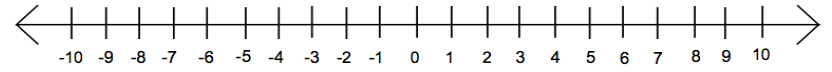
\includegraphics[width=\textwidth]{Sections/FunctionsandGraphsImages/Figure01.png}
	\caption{A visualization of all real numbers}
\end{figure}

\begin{figure}[H]
	\centering
	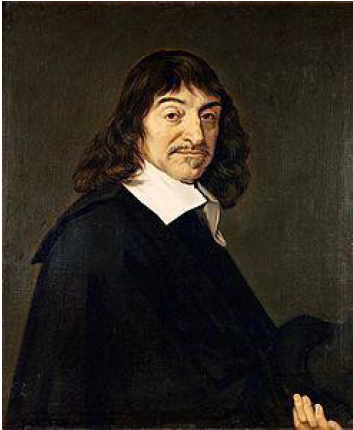
\includegraphics[scale=1.0]{Sections/FunctionsandGraphsImages/Figure02.png}
	\caption{Descartes: He thought, therefore he was. Source: wikipedia.org}
\end{figure}

Descartes’ innovation was to draw two number lines, one perpendicular to the other, to create a plane, called the \textbf{coordinate plane}\index{Coordinate Plane}, or, in his honor, the \textbf{Cartesian plane}\index{Cartesian Plane} \footnote{\quotes{Cartesian} is derived from the name \quotes{Descartes}. The \quotes{Des} is left off for reasons having to do with the Latin form of his name.}. The horizontal number line is used to represent all the possible input values of a function. It is known as the \textbf{horizontal axis, or the input axis}\index{Coordinate Plane!Horizontal Axis}, or, since the most common variable name to use for inputs is $x$, the \textbf{$x$-axis}.\\

The output values for the function are represented using the vertical number line, known as the \textbf{vertical axis, or output axis}\index{Coordinate Plane!Vertical Axis}, or, since the most common variable name to use for outputs is $y$, \textbf{the $y$-axis}.

\begin{figure}[H]
	\centering
	%should be scaled down
	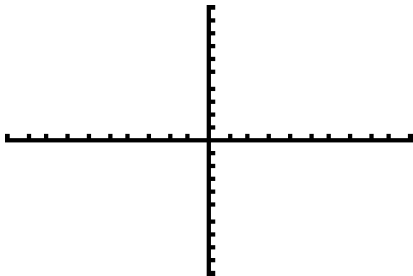
\includegraphics[scale=1.0]{Sections/FunctionsandGraphsImages/Figure03.png}
	\caption{A set of coordinate axes.}
\end{figure}

Any coordinate pair can be represented as a point in this plane. The $x$ and $y$ values of the coordinate pair give its point’s location. We move right or left along the $x$-axis to the $x$ value, and then from there we move up or down parallel to the $y$-axis to the $y$ value. For example, the coordinate pair $(3, -2)$ would be represented by the point in the plane shown below:

\begin{figure}[H]
	\centering
	%should be scaled down
	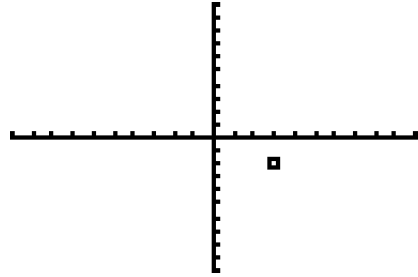
\includegraphics[scale=1.0]{Sections/FunctionsandGraphsImages/Figure04.png}
	\caption{The point $(3,-2)$ marked on a set of axes.}
\end{figure}

Now, we can represent any numerical table as a collection of points in the plane. The table we create above, giving a few selected inputs and outputs for the function $f(x)=2x$ could be represented by the following points in the plane:

\begin{figure}[H]
	\centering
	%should be scaled down
	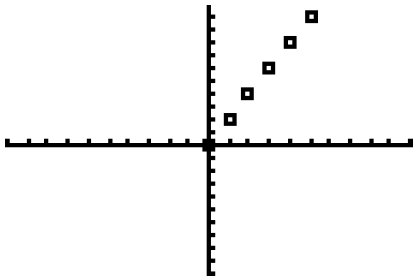
\includegraphics[scale=1.0]{Sections/FunctionsandGraphsImages/Figure05.png}
	\caption{Some input-output pairs for $f(x)=2x$.}
\end{figure}

Now here’s the infinitely clever part. If we want to represent all the input-output pairs for a function, we can actually do that. Notice that the points we plotted for $f(x)=2x$ in the diagram above all seem to fall into a pattern – they seem to fall in a straight line. It turns out that if we plotted all the input-output pairs for $f(x)=2x$ they would form a straight line like this:

\begin{figure}[H]
	\centering
	%should be scaled down
	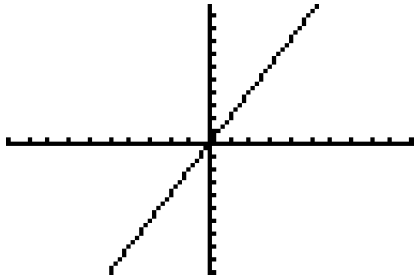
\includegraphics[scale=1.0]{Sections/FunctionsandGraphsImages/Figure06.png}
	\caption{The line formed by input-output pairs for $f(x)=2x$.}
\end{figure}

Note that for the time being, you’ll have to take it on faith that all the input-output pairs for this function actually do fall into this line; in the next chapter we’ll see how we know for sure that the input-output pairs are precisely the same as the points on the line. It should though seem
reasonable to expect there is something more than just a coincidence going on that the points we plotted happen to fit a straight line.\\

For many functions, the points for all the input-output pairs will form straight lines like this one. There are other possibilities, however. For example, if we consider the function $g(x)=x^2$ we can create this table:

\begin{center}
	\begin{tabular}{c|c|c|c|c|c|c|c}
		$x$ & -3 & -2 & -1 & 0 & 1 & 2 & 3\\
		\hline
		$g(x)$ & 9 & 4 & 1 & 0 & 1 & 4 & 9
	\end{tabular}
\end{center}

and if we plot the points from this table in the plane we get:

\begin{figure}[H]
	\centering
	%should be scaled down
	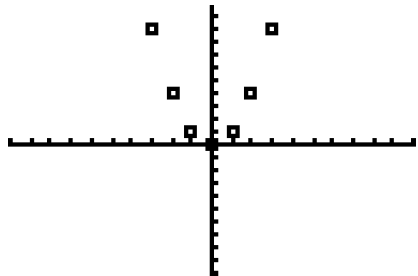
\includegraphics[scale=1.0]{Sections/FunctionsandGraphsImages/Figure07.png}
	\caption{Some of the input-output pairs for the function $g(x)=x^2$.}
\end{figure}

which clearly can’t be made to fit any straight line. It turns out (again, we’ll see exactly why this is later) that the actual collection of points for this function looks like this:

\begin{figure}[H]
	\centering
	%should be scaled down
	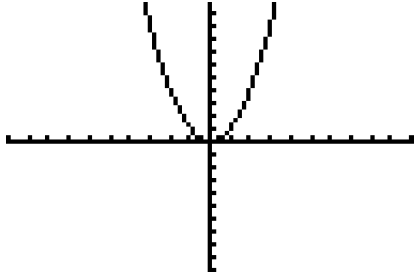
\includegraphics[scale=1.0]{Sections/FunctionsandGraphsImages/Figure08.png}
	\caption{The shape formed by the input-output pairs for $g(x)=x^2$.}
\end{figure}

Even though that’s not a straight line, it definitely fits a pattern. That’s huge. It turns out that when we plot all the points for all the input-output pairs for just about any function we might care about, the result will always be some reasonable shape or pattern.\\

The collection of all the input-output pairs for a function plotted in a coordinate plane is called a \textbf{graph}\index{Graph} of the function. We will see in the upcoming chapters of this book that graphs are an incredibly powerful tools for working with functions.\\

Before moving on, there are a few terms that are commonly used with graphs and the coordinate plane that we should define. The point $(0,0)$ that lies in the center where the two axes intersect is called the \textbf{origin}\index{Coordinate Plane!Origin}. You can think of the origin as the \quotes{starting point} from which we move to the
coordinates of other points.\\

Also, the two axes naturally divide the coordinate plan into four quarters, which are called \textbf{quadrants}\index{Coordinate Plane!Quadrants}. The quadrants are numbered, usually with Roman numerals, starting in the upper right and moving around counter-clockwise, as shown below:

\begin{figure}[H]
	\centering
	%should be scaled down
	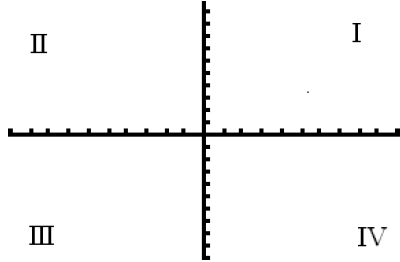
\includegraphics[scale=1.0]{Sections/FunctionsandGraphsImages/Figure09.png}
	\caption{The quadrants of the Cartesian Plane.}
\end{figure}

Quadrant I is called the \textbf{first quadrant}, quadrant II is called the \textbf{second quadrant}, etc.\\

\exam{\label{FunctionsandGraphsExample5}Sketch the location of the point $(-3,1)$ in the Cartesian plane. In which quadrant is this point located?}

\indenttext{To locate this point we follow the input (horizontal) axis from the origin to the left to $-3$ and then follow the output (vertical) axis up to a height of $+1$.

	\begin{figure}[H]
		\centering
		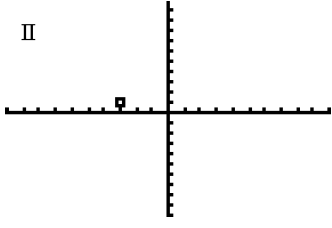
\includegraphics[scale=1.0]{Sections/FunctionsandGraphsImages/Figure10.png}
		\caption{The location of $(-3,1)$ in the Cartesian Plane}
	\end{figure}

	This point lies in the second quadrant (i.e. Quadrant II).
}

\exam{\label{FunctionsandGraphsExample6}Sketch the location of the point $(0,-2)$ in the Cartesian plane. In which quadrant is this point located?}

\indenttext{Because the first coordinate is $0$, we don’t move at all to the right or left from the origin. We then follow the output (vertical) axis down to $-2$.
	\begin{figure}[H]
		\centering
		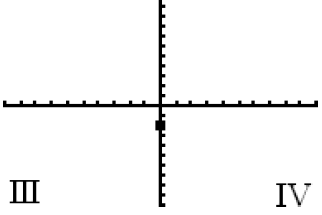
\includegraphics[scale=1.0]{Sections/FunctionsandGraphsImages/Figure11.png}
		\caption{The location of $(0,-2)$ in the Cartesian Plane}
	\end{figure}
	This point does not lie in any quadrant. It is located directly on the output (vertical) axis between Quadrants III and IV.
}

\bigskip

We can create graphs for functions whose formulas we know (more on that later). We can also, though, use graphs even without formulas as a way of describing functions. For example, suppose you are filling a tub with water at a steady rate. The amount of water in the tub is a function of the time (since at any given time there is one and only one amount of water in the tub). Can we sketch a graph of what this function would look like?\\

If we assume the starting time (when \quotes{time is zero}) is when we first started the water flowing in, we know that the graph must include the origin, since when the time is zero (i.e. when we start) the amount of water in the tub is also zero (i.e. the tub is empty). Then as time passes, the amount of water goes up at a steady rate, so our graph should also go up at a steady rate until the tub is full, at which point the graph would level off. So, the graph should look something like this:

\begin{figure}[H]
	\centering
	%should be scaled down
	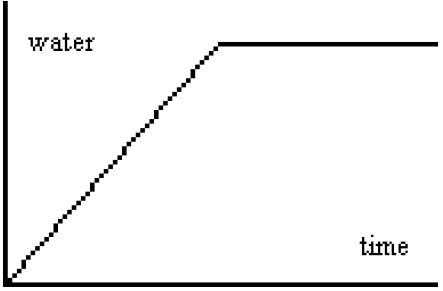
\includegraphics[scale=1.0]{Sections/FunctionsandGraphsImages/Figure12.png}
	\caption{Graph of water in the tub as a function of time}
\end{figure}

Now, we can’t put numbers on this graph because we don’t have that information; we don’t know the rate of the water’s flow, the volume of the tub, how long it took to fill, etc. But we can label the axes with the quantities each axis represents, and we can feel confident that this graph communicates the idea of filling the tub at a steady rate.\\

Notice that in this graph we only are looking at the first quadrant. This is because our interest lies only with positive values of the variables. We are not interested in the amount of water in the tub before we begin to fill it, and there could never be negative amount of water in the tub. Of course we could include show those empty quadrants if we wanted to for some reason, but doing so would serve no purpose.\\

When using a graph to describe a function you should always label the graph with as much relevant information as you have available. At a minimum, the axes should always be labeled. If other information is available, that may be included as well.

\exam{\label{FunctionsandGraphsExample7}A radioactive isotope of iodine decays with a half life of 8 hours (that is, one half of the isotope decays every 8 hours). A lab has a 20 gram sample of this isotope. Sketch a graph of the remaining amount of the isotope as a function of time.}

\indenttext{The amount is decreasing, so our graph should move downward. It cannot move down in a straight line, though, because if it did the graph would eventually fall below the horizontal axis – meaning a negative amount of iodine, which is ridiculous. So, the graph must curve downward.\\

	We can get a sense of how this would work by plotting a few points based on the information we have. Since the amount is reduced by half every 8 hours, we can figure out the amounts we have at 8 hour intervals:\\

	\begin{center}
		\begin{tabular}{c|c}
			Time (hours) & Amount (grams) \\
			\hline
			0 & 20\\
			8 & 10 \\
			16 & 5 \\
			24 & 2.5
		\end{tabular}
	\end{center}

	Roughly plotting these points:

	\begin{figure}[H]
		\centering
		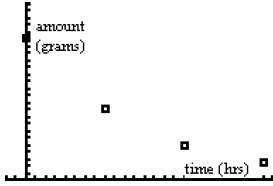
\includegraphics[scale=1.0]{Sections/FunctionsandGraphsImages/Figure13.png}
		%\caption{}
	\end{figure}

	gives us a sense of what the graph must look like. Connecting these dots into a smooth shape and labeling we should end up with a graph something like this:

	\begin{figure}[H]
		\centering
		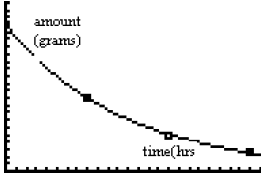
\includegraphics[scale=1.0]{Sections/FunctionsandGraphsImages/Figure14.png}
		%\caption{}
	\end{figure}

	It is not necessary and probably not even desirable to show all the plotted points specifically labeled; but it would be good to label a few values to give a sense of scale. A graph such as this would be a good choice:

	\begin{figure}[H]
		\centering
		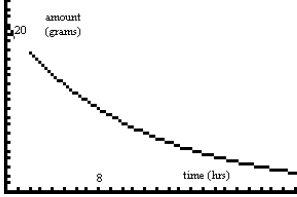
\includegraphics[scale=1.0]{Sections/FunctionsandGraphsImages/Figure15.png}
		%\caption{}
	\end{figure}
}

Graphs can take on all sorts of shapes. For example, here is graph for the closing price of the Dow Jones Industrial Average (a reflection of the US stock market) as a function of time over the years 2008-2009:

\begin{figure}[H]
	\centering
	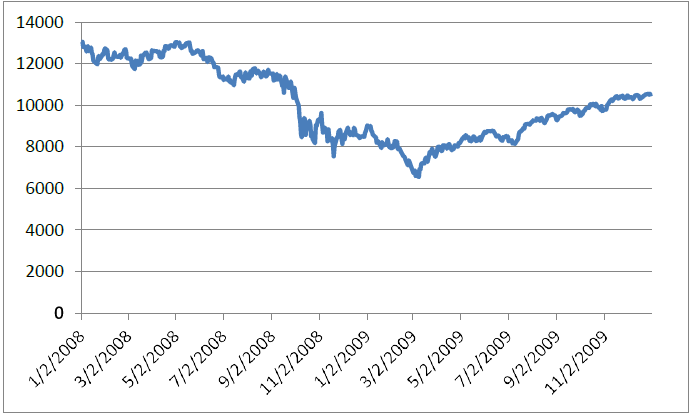
\includegraphics[scale=1.0]{Sections/FunctionsandGraphsImages/Figure16.png}
	%\caption{}
\end{figure}

And of course wilder shapes are possible. Is there any restriction on what shapes a graph can take? Well, what about a \quotes{graph} like this one:

\begin{figure}[H]
	\centering
	%should be scaled down
	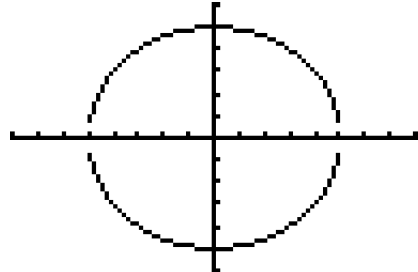
\includegraphics[scale=1.0]{Sections/FunctionsandGraphsImages/Figure17.png}
	\caption{Could this be a graph of a function?}
\end{figure}

This is a nice, smooth, geometrically pretty shape. Shapes don’t come much nicer than circles. But could it be the graph of a function? Well, no, actually. Remember that a function must give \underline{one and only one} output for each input in its domain.\\

The input $x=6$ does not have an output here, but that is fine if this were the graph of a function. That just means $6$ is not in the domain. The problem lies with inputs like $x=3$. What is the output for the input $x=3$?  Well based on where the marks on the axis are located, it looks as though the point $(3,4)$ is on the graph, so we might think the output must be $y=4$. Or, in other words, $f(3)=4$. But the point $(3,-4)$ is also appears to be on the graph, so the output for $x=3$ must also be $y=-4$. Or in other words, $f(3)=-4$ too. And that is a problem. Remember, a function must always give a straight answer! For the input $x=3$ the \quotes{graph} cannot show two different outputs. Therefore this circle cannot be the graph of a function.\\

There’s nothing special about the input $x=3$. We could have used lots of other choices for $x$ and run into the same problem. In fact, we could have used any input where the graph shows to different outputs. We don’t even need to be able to tell what the specific outputs are. If we used the input $x=-2.5$, say, we might not be able to tell very well what the corresponding outputs are, but we could tell that there are two of them.

\begin{figure}[H]
	\centering
	%should be scaled down
	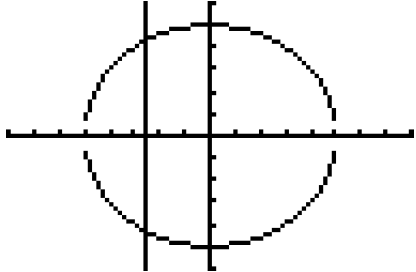
\includegraphics[scale=1.0]{Sections/FunctionsandGraphsImages/Figure18.png}
	\caption{Drawing a vertical line shows how the input value we've drawn it through has two outputs}
\end{figure}

The observation we are making here is sometimes referred to as the vertical line test.

\begin{definition}
	\index{Vertical Line Test}
	\textbf{\underline{The Vertical Line Test}}\\
	\bigskip
	A graph is the graph of a function if, and only if,\\ you can never draw a vertical line which intersects the graph more than once.\\
	\bigskip
	OR equivalently\\
	\bigskip
	A graph is the graph of a function if, and only if, \\ every vertical line you can draw will intersect the graph at most one time.
\end{definition}

Because the only requirement of a function is that it give one and only one output for each input, the only requirement for a graph to be a function is the vertical line test.

%%%%%%%%%%%%%%%%%%%%%%%%%%%%%%%%%%%%%%%%%%%%%%%%%%%%%%%%%%%%
%
% Subsection: Graphing Calculator
%
%%%%%%%%%%%%%%%%%%%%%%%%%%%%%%%%%%%%%%%%%%%%%%%%%%%%%%%%%%%%

\subsection{The Graphing Calculator}

Throughout this course, we will be using graphs extensively. A graphing calculator is required for this course, and before we conclude this section we will introduce the use of the calculator to obtain graphs of functions when we know their formulas. (We’ll just introduce the basics here, and expand on the use of the graphing calculator in future chapters.)\\

Let’s return to the function we started this chapter with, $f(x)=2x$. We can use the calculator to obtain a graph of this function using the following process.\\

\index{Calculator:Graphing}\textbf{Step 1: Enter the function formula into the calculator.} We first need to tell the calculator the formula for the function we want to graph. (We do this the same way that we entered formulas to create tables in Chapter ??.) First, hit the \quotes{Y=} key in the upper left corner of your TI-83 or 84, and then enter the formula on the first (\quotes{Y1=}) line. As with tables, the other lines (\quotes{Y2=}, \quotes{Y3=} etc.) are there to allow you to enter more than one formula at a time – not something we care about right now. Also as with tables, the formula must be written with \quotes{X} as the input variable. Use the \quotes{X,T,$\Theta$,n} key to get an \quotes{X}. The resulting screen should look like this:

\begin{figure}[H]
	\centering
	%should be scaled down
	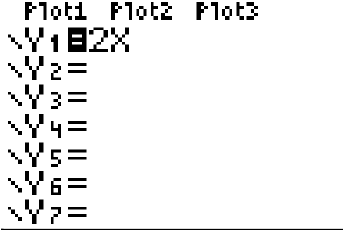
\includegraphics[scale=1.0]{Sections/FunctionsandGraphsImages/Figure19.png}
	%\caption{}
\end{figure}

\index{Calculator:Window Settings} \textbf{Step 2: Set the window.} The Cartesian plane extends out to infinity in all directions, and many graphs do as well. So of course there is no way to display the whole plane on the calculator screen.  We need to tell the calculator what portion of the plane we want it to display. \\

In the calculator’s top row there is a key labeled \quotes{WINDOW}. Hit that key now, and it will take you to a screen that should look like this (though the specific numbers you see may not be the same):

\begin{figure}[H]
	\centering
	%should be scaled down
	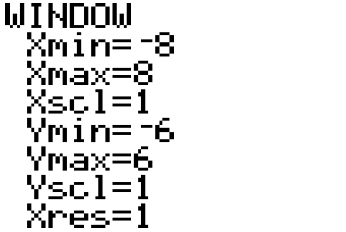
\includegraphics[scale=1.0]{Sections/FunctionsandGraphsImages/Figure20.png}
	%\caption{}
\end{figure}

The \quotes{Xmin} and \quotes{Xmax} tell the calculator the interval of $x$ (input) values to show on the graph. On the screen shown above as an example, the calculator would show the portion of the graph that lies between $x=-8$ and $x=8$. Likewise, the \quotes{Ymin} and \quotes{Ymax} determine the range of $y$ (output) values used; in this window it would be the portion of the graph that lies between $y=-6$ and $y=6$.\\

The \quotes{Xscl} and \quotes{Yscl} determine where the marks on the axes occur. These both being set to 1 tells the calculator to mark both axes in intervals of 1 unit. The \quotes{Xres} helps determine how precisely the calculator sketches the points on the graph; the precise way in which this is used need no concern us right now. We will just leave that at the default of Xres=1.\\

The settings to enter here will depend on what portion of the graph you want to look at in any particular situation. The default, which we’ll use whenever we don’t have reason to look elsewhere, is the standard window, which ranges from $-10$ to $+10$ on both axes, with hashmarks (ticks) every one unit. So, to set things to the standard window, we would want the following settings:

\begin{figure}[H]
	\centering
	%should be scaled down
	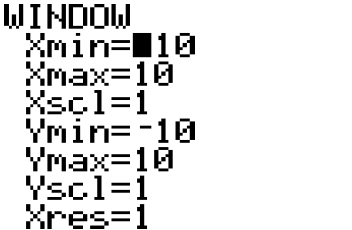
\includegraphics[scale=1.0]{Sections/FunctionsandGraphsImages/Figure21.png}
	%\caption{}
\end{figure}

\textbf{Step 3: Get the graph.} In the upper right corner, you’ll see a key labeled \quotes{GRAPH}. Hit that key now and you should see this:

\begin{figure}[H]
	\centering
	%should be scaled down
	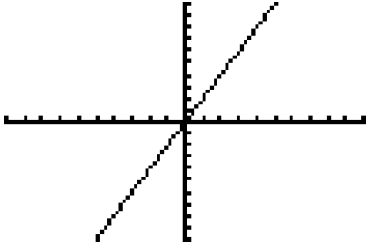
\includegraphics[scale=1.0]{Sections/FunctionsandGraphsImages/Figure22.png}
	%\caption{}
\end{figure}

\index{Calculator:Zoom} As an alternative, when you want a graph in the standard window, you can just hit the \quotes{ZOOM} key in your calculator’s upper row, and select \quotes{6: ZStandard}:

\begin{figure}[H]
	\centering
	%should be scaled down
	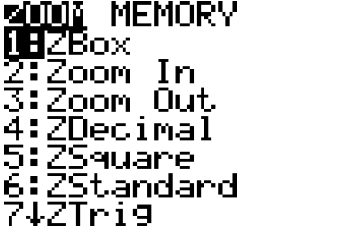
\includegraphics[scale=1.0]{Sections/FunctionsandGraphsImages/Figure23.png}
	%\caption{}
\end{figure}

This will take you directly to the graph in the standard window, essentially combining Step 2 and Step 3.\\

\textbf{It is important to remember that the calculator only shows the portion of the graph that our window instructions tell it to.} It should be apparent that the graph of $f(x)=2x$ continues above and below the graph we generated above. If you wish to see those portions of the graph, you can adjust your window settings and see them. But whether we see them or not, they are there, and while we can’t see them on the calculator’s screen with our actual eyes, we can see them with the mind’s eye. \\

Following these steps, we can now create a graph for just about function defined with a formula.  Our goal is of course not just to admire these graphs’ beauty – we want to use them as a tool, and as we proceed through the course we’ll see more and more how to do this. Before leaving this chapter, though, we’ll mention at least one use for these graphs.\\

Since a function’s graph consists of all its input-output pairs, we can use graphs to find the output for any given input. The calculator allows you to \quotes{walk} along the graph, telling you the coordinates of points you encounter along the way. In the top row of your calculator you will see a key labeled \quotes{TRACE}. If you hit this key, you’ll see a \quotes{blob} placed somewhere on the graph, and the input and output values of its coordinates:

\begin{figure}[H]
	\centering
	%should be scaled down
	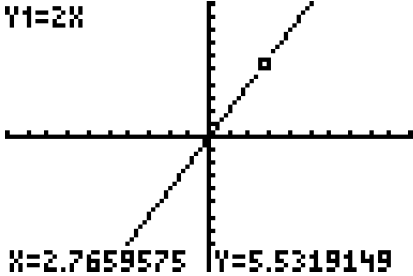
\includegraphics[scale=1.0]{Sections/FunctionsandGraphsImages/Figure24.png}
	%\caption{}
\end{figure}

If you don’t see the coordinate values, hit \quotes{2nd} \quotes{ZOOM} (that is, \quotes{FORMAT}) and make sure your settings are like this:

\begin{figure}[H]
	\centering
	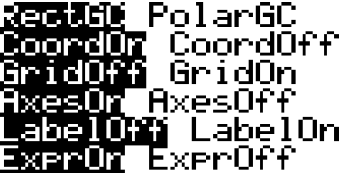
\includegraphics[scale=1.0]{Sections/FunctionsandGraphsImages/Figure25.png}
	%\caption{}
\end{figure}

You can now move around to different points on the graph by using the right and left directional keys in the upper right portion of your calculator.\\

As you do this you’ll notice that not every point on the graph is visited when you trace. That can’t be avoided – there are infinitely many points on the graph, so there’s no way you could visit them all! To visit the point on the graph associated with a given input value, hit \quotes{2nd} \quotes{TRACE} (that is, \quotes{CALC}) in the top row to get this menu:

\begin{figure}[H]
	\centering
	%should be scaled down
	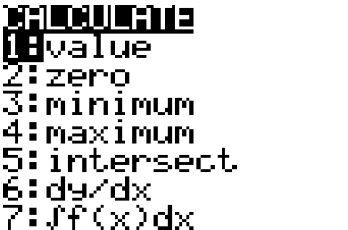
\includegraphics[scale=1.0]{Sections/FunctionsandGraphsImages/Figure26.png}
	%\caption{}
\end{figure}

Select \quotes{1: value} and you’ll be returned to the graph with a screen that looks like this:

\begin{figure}[H]
	\centering
	%should be scaled down
	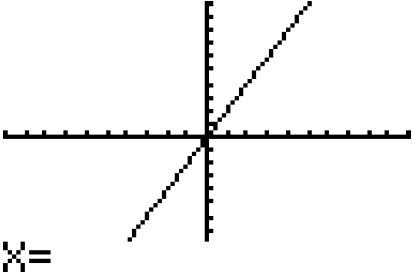
\includegraphics[scale=1.0]{Sections/FunctionsandGraphsImages/Figure27.png}
	%\caption{}
\end{figure}

Now you can enter the input ($x$) value you want to visit. If we want, say, to visit the point that goes with $x=-3$ we get:

\begin{figure}[H]
	\centering
	%should be scaled down
	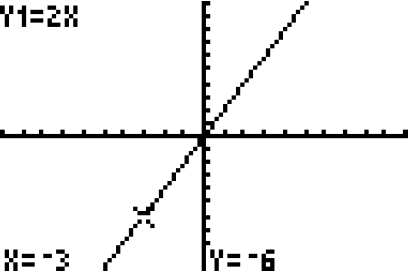
\includegraphics[scale=1.0]{Sections/FunctionsandGraphsImages/Figure28.png}
	%\caption{}
\end{figure}

\exam{\label{FunctionsandGraphsExample8}Obtain a graph for $h(t)=\frac{t^3+3t^2}{12}$ in the standard window, and use this graph to find $h(2)$}

\indenttext{Following the steps outlined above, we first need to enter the function’s formula into the calculator.  Recall that the calculator only understands X as the input value, so we need to rewrite that formula replacing the $t$ with an X:

	\begin{figure}[H]
		\centering
		%should be scaled down
		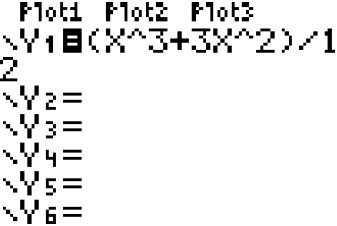
\includegraphics[scale=1.0]{Sections/FunctionsandGraphsImages/Figure29.png}
		%\caption{}
	\end{figure}

	Now, either directly adjusting the window setting to the standard window and hitting \quotes{GRAPH}, or just using \quotes{ZOOM} --> \quotes{6: ZStandard}, we get:

	\begin{figure}[H]
		\centering
		%should be scaled down
		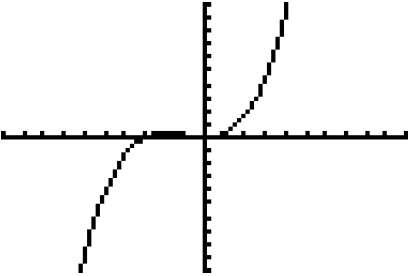
\includegraphics[scale=1.0]{Sections/FunctionsandGraphsImages/Figure30.png}
		%\caption{}
	\end{figure}

	Then using \quotes{2nd} \quotes{TRACE} (that is, \quotes{CALC}) --> \quotes{1: value} and entering \quotes{X=2} we get:

	\begin{figure}[H]
		\centering
		%should be scaled down
		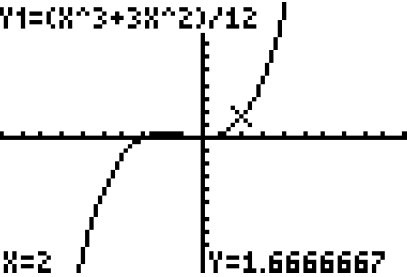
\includegraphics[scale=1.0]{Sections/FunctionsandGraphsImages/Figure31.png}
		%\caption{}
	\end{figure}

	So, we conclude that $h(2)=1.6666667$ which we would either recognize as $h(2)=\frac{5}{3}$ or round t0 something reasonable such as $h(2) = 1.67$.
}

%%%%%%%%%%%%%%%%%%%%%%%%%%%%%%%%%%%%%%%%%%%%%%%%%%%%%%%%%%%%
%
% Functions and Graphs Exercises
%
%%%%%%%%%%%%%%%%%%%%%%%%%%%%%%%%%%%%%%%%%%%%%%%%%%%%%%%%%%%%

\clearpage

\subsection{Exercises}

\subsubsection*{Coordinates}
\ex{Rewrite the function given in the table below as a set of coordinate pairs.
	\begin{center}
		\begin{tabular}{|c|c|c|c|c|c|}
			\hline
			$x$ & 1 & 2 & 4 & 8 & 12 \\
			\hline
			$g(x)$ & 2 & 2 & 7 & 1 & 0\\
			\hline
		\end{tabular}
	\end{center}
} \sol{$\{(1,2), (2,2), (4,7), (8,1), (12,0)\}$}

\bigskip
\ex{Rewrite the function given in the table below as a set of coordinate pairs.
	\begin{center}
		\begin{tabular}{|c|c|c|c|c|c|}
			\hline
			$t$ & 0 & -3 & 6 & 4 & 3 \\
			\hline
			$h(t)$ & 5 & 7 & 6 & 11 & -1\\
			\hline
		\end{tabular}
	\end{center}
}

\bigskip
\ex{Suppose $f(2) = -1$. Express this as a coordinate pair.} \sol{$(2, -1)$}

\bigskip
\ex{Suppose $g(0) = 3$. Express this as a coordinate pair.}

\bigskip
\ex{Rewrite the function given by the following set of coordinate pairs as a table, assume $f(x)$: $\{(1,3), (2,5), (3,-1), (5,-2)\}$.}
\sol{
	$$ \begin{array}{c|c}
		x & f(x) \\
		\hline
		1 & 3 \\
		2 & 5 \\
		3 & -1 \\
		5 & -2 \\
	\end{array} $$}

\bigskip
\ex{Rewrite the function given by the following set of coordinate pairs as a table, assume \( g(t) \): $\{(1,5), (2,-1), (4,6), (7,-3)\}$.}

\bigskip
\ex{The coordinate pair $(5,3)$ gives an input and output for the function $f(x) $.  Does this mean $f(3)=5$ or that $f(5) = 3$?} \sol{$f(5)=3$}

\bigskip
\ex{The coordinate pair $(2, -7)$ gives an input and output for the function $g(t) $. Does this mean $g(2) = -7$ or $g(-7)=2$?}

\bigskip
\ex{Is $\{(0,2), (-1,3), (1, -3), (2,8), (-2, -8)\} $ a function? Why or why not?} \sol{Yes, each input has one and only one corresponding output.}

\bigskip
\ex{Is $\{(0,5), (2,3), (2,5), (4,6), (4,8)\}$ a function? Why or why not?}

\bigskip
\ex{Is $\{(1,1), (2,1), (3,1)\} $ a function?  Why or why not?} \sol{Yes, each input has one and only one corresponding output.}

\bigskip
\ex{Is $\{(1,1), (1,2), (1,3)\} $ a function?  Why or why not?}

\bigskip
\ex{Is $\{(0,0), (0,1), (1,2), (2,3), (3,4)\} $ a function?  Why or why not?}  \sol{No, because the input $0$ has two different outputs ($0$ and $1$).}

\bigskip
\ex{Is $\{(-1,2), (-2,2), (-3,2), (-4,2)\} $ a function?  Why or why not?}

\subsubsection*{Graphs}

\ex{Use your calculator to create a table of values for the function $f(x)=(x+1)(x-1)$ for the inputs $x = -3, -2, -1, 0, 1, 2, 3 $ or create the table yourself by hand.  Then sketch a coordinate plane and plot these points on it.  Use the points you plotted to sketch what the graph of $f(x)$ appears to be.}
\sol{
	$$
	\begin{array}{c|c}
		x & f(x) \\
		\hline
		-3 & 8 \\
		-2 & 3 \\
		-1 & 0 \\
		0 & -1 \\
		1 & 0 \\
		2 & 3 \\
		3 & 8 \\
	\end{array}
	$$
	\begin{figure}[H]
		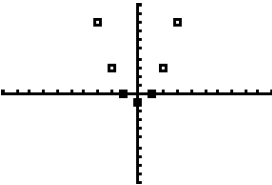
\includegraphics[scale=1.0]{Sections/FunctionsandGraphsImages/Answer15a.png}
	\end{figure}
	\begin{figure}[H]
		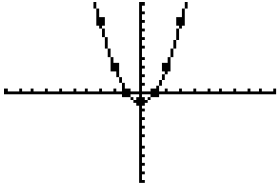
\includegraphics[scale=1.0]{Sections/FunctionsandGraphsImages/Answer15b.png}
\end{figure}}
\bigskip

\ex{Use your calculator to create a table of values for the function $f(x)=x-3(x-1)$ for the inputs $x = -3, -2, -1, 0, 1, 2, 3 $ or create the table yourself by hand.  Then sketch a coordinate plane and plot these points on it.  Use the points you plotted to sketch what the graph of $f(x)$ appears to be.}
\bigskip

\ex{Sketch the location of each of the following points in the Cartesian plan, and state the quadrant in which each is located.
	\begin{enumerate}[label=(\alph*)]
		\item $(2,1)$
		\item $(-1,2)$
		\item $(5,-1)$
		\item $(0,2)$
	\end{enumerate}
}
\sol{
	\begin{enumerate}[label=(\alph*)]
		\item First quadrant
		\begin{figure}[H]
			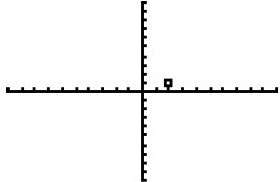
\includegraphics[scale=1.0]{Sections/FunctionsandGraphsImages/Answer17a.png}
		\end{figure}
		\item Second quadrant
		\begin{figure}[H]
			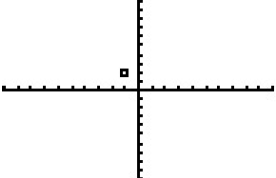
\includegraphics[scale=1.0]{Sections/FunctionsandGraphsImages/Answer17b.png}
		\end{figure}
		\item Fourth quadrant
		\begin{figure}[H]
			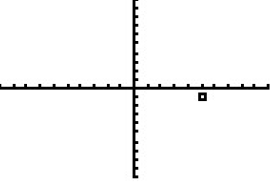
\includegraphics[scale=1.0]{Sections/FunctionsandGraphsImages/Answer17c.png}
		\end{figure}
		\item none, between first and second quadrants
		\begin{figure}[H]
			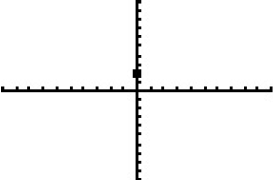
\includegraphics[scale=1.0]{Sections/FunctionsandGraphsImages/Answer17d.png}
		\end{figure}
	\end{enumerate}
}

\bigskip
\ex{Sketch the location of each of the following points in the Cartesian plan, and state the quadrant in which each is located.
	\begin{enumerate}[label=(\alph*)]
		\item $(-3,1)$
		\item $(1,-3)$
		\item $(-1,-3)$
		\item $(-2,0)$
	\end{enumerate}
}

\bigskip
\ex{Sketch a possible graph for each of the functions described. Label your axes, and, if available, include any other relevant information in your graph as well.
	\begin{enumerate}[label=(\alph*)]
		\item the remaining balance on a mortgage as a function of time as the loan is being paid
		\item the monthly sales of hybrid cars as a function of the price per gallon of gasoline
		\item the height of a sunflower as a function of time since the seed was planted 
	\end{enumerate}
}
\sol{Possible graphs, answers will vary
	\begin{enumerate}[label=(\alph*)]
		\item \phantom{a}
		\begin{figure}[H]
			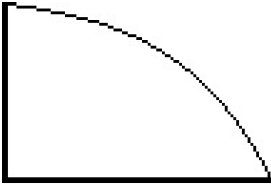
\includegraphics[scale=1.0]{Sections/FunctionsandGraphsImages/Answer19a.png}
		\end{figure}
		\item \phantom{b}
		\begin{figure}[H]
			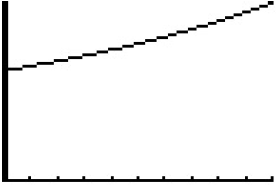
\includegraphics[scale=1.0]{Sections/FunctionsandGraphsImages/Answer19b.png}
		\end{figure}
		\item \phantom{c}
		\begin{figure}[H]
			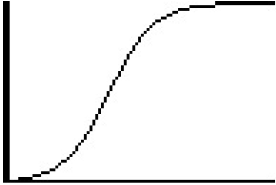
\includegraphics[scale=1.0]{Sections/FunctionsandGraphsImages/Answer19c.png}
		\end{figure}
	\end{enumerate}
}

\bigskip
\ex{Sketch a possible graph for each of the functions described. Label your axes, and, if available, include any other relevant information in your graph as well.
	\begin{enumerate}[label=(\alph*)]
		\item the height of a ball as a function of time since it was thrown upward
		\item the risk of a heart attack as a function of a man’s weight
		\item the amount of oil in a reservoir as a function of time since production from the reservoir began 
	\end{enumerate}
}

\bigskip
\ex{For each of the given scenarios, make a reasonable sketch of what the graph of noise in the college’s basketball area as function of time might look like:
	\begin{enumerate}[label=(\alph*)]
		\item Everyone was excited at the start of the game, since the two teams were bitter rivals in close competition for the league championship. The first half was close, with the two teams pretty well matched and neither team able to get much of a lead. But in the second half, the home team quickly fell behind and never even got close again, finally losing by 18 points.
		\item No one really expected much from this game, since the visiting team was heavily favored, but the home team hung in there and kept the game close through the first half and the first part of the second half. But then the home team had a terrific run and broke away to a 7 point lead. The visitors came back and made it close, taking the lead again just before the buzzer, but the home team put the game away on a last second 3 pointer.
		\item The visiting team already had the league championship locked up, and for the home team this was the last game of a disappointing season. The visitors quickly built up a sizeable lead, and the game never was even competitive.
\end{enumerate} }
\sol{There are many possible answers, but all should show the noise level getting higher when the game is more exciting and lower when the game is less exciting}

\bigskip
\ex{For each of the given scenarios, make a reasonable sketch of what the graph of Zarofire Systems’ stock price might look like as a function of time:
	\begin{enumerate}[label=(\alph*)]
		\item The stock began the year at a price of \$2 per share, and stayed pretty much flat for several months. Then the company reported blow out earnings, and the stock price quickly soared to new highs, after which it continued to rise gradually for the next few months, before leveling off through the end of the year and ending the year at \$10 per share.
		\item The stock began the year at around \$2 per share, and over the first few months of the year slowly and gradually faded downward. About mid–year it started to move upward again for a month or so, approaching but not quite returning to where it started the year, and then leveled off for a few months. Finally, the company unexpectedly filed for bankruptcy, and on that news the stock fell dramatically and ended the year nearly worthless.
		\item The stock began the year at around \$2 per share, and gradually wavered between \$1.75 and \$2.25 for the first half of the year. A bit past midyear, the company received a buyout offer at \$5 per share, and the stock immediately shot up to nearly that price, where it remained until the deal was completed at year’s end.
\end{enumerate} }

\bigskip
\ex{Which of the following could be the graph of a function? Explain your reasoning.
\begin{tabular}{lll}
	a. 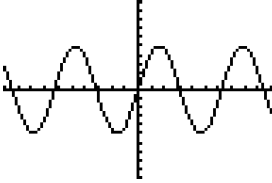
\includegraphics[scale=0.6]{Sections/FunctionsandGraphsImages/Question23a.png}
	&  	
	b. 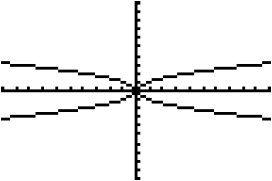
\includegraphics[scale=0.6]{Sections/FunctionsandGraphsImages/Question23b.png}
	&
	c. 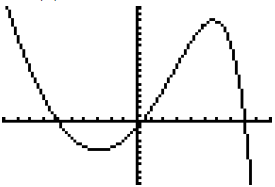
\includegraphics[scale=0.6]{Sections/FunctionsandGraphsImages/Question23c.png}
\end{tabular}
}
\sol{a. is a function  b. is not a function  c. is a function }

\bigskip
\ex{Which of the following could be the graph of a function? Explain your reasoning.
\begin{tabular}{lll}
	a. 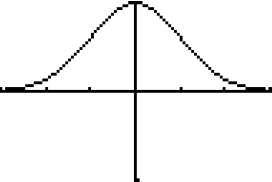
\includegraphics[scale=0.6]{Sections/FunctionsandGraphsImages/Question24a.png}
	&  	
	b. 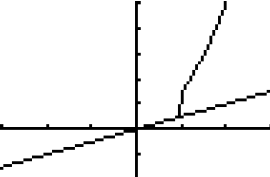
\includegraphics[scale=0.6]{Sections/FunctionsandGraphsImages/Question24b.png}
	&
	c. 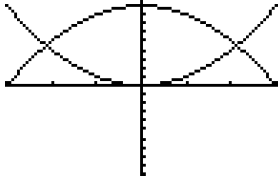
\includegraphics[scale=0.6]{Sections/FunctionsandGraphsImages/Question24c.png}
\end{tabular}
}

\subsubsection*{Graphing Calculator}

\ex{Use your calculator to obtain a graph for $f(x)=5-x$ in the standard window. Use your graph to find $f(2.4)$, $f(-1.3)$, and $f(-7.2)$.}
\sol{$f(2.4)=2.6$, $f(-1.3)=6.3$, and $f(-7.2)=12.2$}

\bigskip
\ex{Use your calculator to obtain a graph for the function $g(x)=7-x/2$ in the standard window. Use your graph to find $g(-3.2)$, $g(1.8)$ and $g(-9.8)$.}

\bigskip
\ex{Use your calculator to create a graph for the function whose graph you sketched in Exercise $15$. Does the calculator’s graph agree with your sketch?}
\sol{The graph should match. (The scale may be different.)}

\bigskip
\ex{Use your calculator to create a graph for the function whose graph you sketched in Exercise $16$. Does the calculator’s graph agree with your sketch?}

\bigskip
\ex{Use your calculator to obtain a graph for the function $h(t)=-16t^2+64t+5$ in the window $0 \leq t \leq 4, 0 \leq h(t) \leq 160$. Use your graph to find $h(1.75)$ and $h(3.8)$.}
\sol{$h(1.75)=68$ and $h(3.8)=17.16$}

\bigskip
\ex{Use your calculator to obtain a graph for the function $j(s)=-4.9s^2+19.6s+2$ in the window $0 \leq s \leq 4, 0 \leq j(s) \leq 75$. Use your graph to find $j(1.75)$ and $j(3.8)$.}

\subsubsection*{Grab Bag}

\ex{If possible, give a value for $q$ that would make the following set of coordinate pairs a function: $\{(0,13), (1,9), (2,14), (q, 9)\}$. If it is not possible to do this, explain.}
\sol{You can use any value except $q=0$ or $q=2$.  If you used $q=1$, then you would have a redundant pair $(1,9)$, but it would still be a function.}

\bigskip
\ex{If possible, give a value for $q$ that would make the following set of coordinate pairs not a function: $\{(0,13), (1,9), (2,14), (q, 9)\}$. If it is not possible to do this, explain.}

\bigskip
\ex{If possible, give a value for $x$ that would make the following set of coordinate pairs a function: $\{(0,1), (1,5), (x, 1)\}$. If it is not possible to do this, explain.}
\sol{You can use any value except $x=1$.}

\bigskip
\ex{If possible, give a value for $x$ that would make the following set of coordinate pairs not a function: $\{(0,1), (1,5), (x, 1)\}$. If it is not possible to do this, explain.}

\bigskip
\ex{Sketch a possible graph for $s(t)$, the speed of your car as a function of time since you got on the thruway.}
\sol{There are several possibilities, but any such graph should show you speeding up when getting on the thruway.  Here is one possibility:
	\begin{figure}[h]
		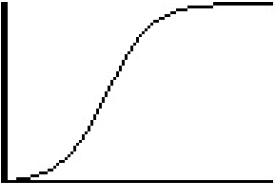
\includegraphics[scale=1.0]{Sections/FunctionsandGraphsImages/Answer35.png}
	\end{figure}
}

\bigskip
\ex{Use your calculator to obtain a graph for $f(x)=10-\frac{x^2}{10}$ in the standard window. Use your graph to find $f(3)$, $f(-5)$, and $f(-8.2)$.}

\bigskip
\ex{Sketch a possible graph for the temperature inside an oven as a function of time since the oven was turned on.}
\sol{There are several possibilities, but any such graph should show the oven starting at room temperature and heating up to the set temperature and pretty much staying at that temperature.  Here is one possible graph:
	\begin{figure}[h]
		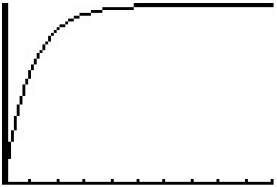
\includegraphics[scale=1.0]{Sections/FunctionsandGraphsImages/Answer37.png}
	\end{figure}
}

\bigskip
\ex{Sketch a possible graph for the temperature inside a hot oven as a function of time since
	the oven was turned off.}

\bigskip
\ex{Use your calculator to obtain a graph for $g(t)=t^3$ in the window $-3 \leq t \leq 3, -50 \leq g(t) \leq 50$}
\sol{The graph
	\begin{figure}[h]
		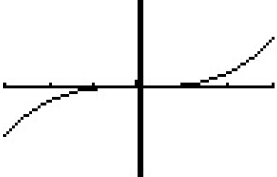
\includegraphics[scale=1.0]{Sections/FunctionsandGraphsImages/Answer39.png}
	\end{figure}
}

\bigskip
\ex{Sketch a possible graph for the volume of water in a backyard pool as a function of the depth of the water in the pool.}

\bigskip
\ex{Use your calculator to obtain a graph for in the standard window for $h(t)=\frac{10-3t}{2}$. Use your graph to find $h(8.2)$, $h(0)$, and $h(-9.6)$.}
\sol{The graph
	\begin{figure}[h]
		\includegraphics[scale=1.0]{Sections/FunctionsandGraphsImages/Answer41.png}
	\end{figure}
	$h(8.2)=-7.3$, $h(0)=5$, and $h(-9.6)=19.4$}

\bigskip
\ex{Use your calculator to obtain a graph for $p(w)=w-2^w$ in the window $-2 \leq w \leq 4, -20 \leq p(w) \leq 5$.}

\bigskip
\ex{In January, the temperature in Frostbite Falls never went above $0 \deg C$.  Let $f(t)$ be the temperature there as a function of time since the start of the year. If you were to sketch the graph of $f(t)$ for the month of January, in which quadrant would the graph be located?}
\sol{Quadrant IV}

\bigskip
\ex{An agricultural scientist is developing a new fertilizer for corn. She will be conducting a study where different amounts of this fertilizer are applied to several hundred test plots. The expected yield (in bushels) of corn from a test plot is a function of the amount of fertilizer applied (in pounds). The scientist’s expected results are given in the table below:
	\begin{center}
		\begin{tabular}{|c|c|c|c|c|c|}
			\hline
			Fertilizer (pounds) & 0 & 1 & 2 & 3 & 4\\
			\hline
			Expected Yield (bushels) & 5 & 8 & 9 & 8 & 5\\
			\hline
		\end{tabular}
	\end{center}
	Let $x$ be the amount of fertilizer applied, and let $f(x)$ be the expected yield.
	\begin{enumerate}[label=(\alph*)]
		\item Sketch a graph of this function by plotting the points for the data given in the table and making a reasonable guess about the shape of the graph based on these points.
		\item This table gives expected yield as a function of fertilizer applied. Would the actual yield of corn be a function of fertilizer applied? Why or why not?
\end{enumerate} }

\bigskip
\ex{Suppose $p(t)$ is the population of New York City as a function of time since the start of this year. Would the graph of $p(t)$ pass through the origin? Why or why not?}
\sol{No it would not.  The origin is $(0,0)$, so if the graph pass through this point then $p(0)=0$ meaning the population of NYC was 0 at the beginning of the year.}

\bigskip
\ex{Suppose $d(t)$ is the distance I’ve travelled on a road trip as a function of time since I left my house. Would the graph of $d(t)$ pass through the origin? Why or why not? }

\bigskip
\ex{Which of the following shapes could be the graph of a function? Explain your reasoning.
	\begin{enumerate}[label=(\alph*)]
		\item a circle
		\item a horizontal line
		\item a triangle
		\item a semicircle
		\item a vertical line
\end{enumerate} }
\sol{a horizontal line and a semicircle that is either the top half or the bottom half of a circle (any other semicircle would fail to be a function)}

\bigskip
\ex{Which of the following upper-case letters could be the shape of the graph of a function?  Explain your reasoning. 
	\begin{enumerate}[label=(\alph*)]
		\item V
		\item W
		\item E
		\item O
		\item C
\end{enumerate} }

\bigskip
\ex{Suppose $f(5)=-2$. Express this as a coordinate pair.}
\sol{$(5,-2$)}

\bigskip
\ex{The point $(-3,8)$ is on the graph of $g(t)$. Does this mean $g(8)=-3$? Why or why not.}

\bigskip
\ex{The point $(2,7)$ is on the graph of $f(x)$. Does this mean $f(2)=7$? Why or why not.}
\sol{Yes.  The first value is the input and the second value is the output.}

\bigskip
\ex{$f(2)=3$, $f(3)=5$, and $f(5)=2$. Express this as a set of coordinate pairs.}


\clearpage

%%%%%%%%%%%%%%%%%%%%%%%%%%%%%%%%%%%%%%%%%%%%%%%%%%%%%%%%%%%%
%
% Section: Solving Equations Graphically
%
%%%%%%%%%%%%%%%%%%%%%%%%%%%%%%%%%%%%%%%%%%%%%%%%%%%%%%%%%%%%

\section{Solving Equations Graphically}
\label{SolvingEquationsGraphically}

Graphs are a powerful tool which we will exploit throughout this book. A particularly powerful use for graphs is as a tool to solve equations, particularly in cases where traditional algebra methods would be tedious or ineffective. In this chapter we will introduce this method and discuss when it is - and when it is not - a useful alternative.

%%%%%%%%%%%%%%%%%%%%%%%%%%%%%%%%%%%%%%%%%%%%%%%%%%%%%%%%%%%%
%
% SubSection: Solving Equations Graphically:Graphical Solution
%
%%%%%%%%%%%%%%%%%%%%%%%%%%%%%%%%%%%%%%%%%%%%%%%%%%%%%%%%%%%%

\subsection{Graphical Solution}

We’ll begin this chapter by showing how we could use a graph to solve a fairly simple equation.
Consider, for example, the equation:

\begin{equation*}
	2x-1=7
\end{equation*}

Now, it is not hard to solve this equation with traditional algebra. Add one to both sides, divide by two, and you can quickly conclude that the solution is $x=4$. Fair enough. But we also could have seen this in another way.\\

The algebraic expression on the left side of that equation can be used to define a function, $f(x)=2x-1$. Using the calculator, we can readily obtain a graph of this function (shown below in the standard window):

\begin{figure}[H]
	\centering
	%should be scaled down
	\includegraphics[scale=1.0]{Sections/SolvingEquationsGraphically/Figure01.png}
	\caption{Graph of $f(x)=2x-1$ in the standard window}
\end{figure}

Now, remember that a graph for a function consists of all of its input-output pairs. For example, $(5,9)$ lies on this graph, because when you input $x=5$ into the function $f(x)=2x-1$ the resulting output is $f(5)=9$.\\

Now, solving the equation $2x-1=7$ amounts to asking \quotes{what $x$ value do we need to input into $f(x)=2x-1$ to get $7$ as the resulting output?} We can find this by looking for the point on the graph where the output value is $7$; that is, where $f(x)=7$.\\

We could try to do this by tracing along the graph to get to the point we are seeking, but we can find it more efficiently in another way. If we consider the right side of the equation as also defining a function $g(x)=7$ and graph that function, the result is just a flat horizontal line whose output value stays at $7$ no matter where we go on the input axis (shown below in the standard window):

\begin{figure}[H]
	\centering
	%should be scaled down
	\includegraphics[scale=1.0]{Sections/SolvingEquationsGraphically/Figure02.png}
	\caption{Graph of $g(x)=7$ in the standard window}
\end{figure}

Now, we can graph the right-side function and left-side function together. The \quotes{Y=} screen allows us to enter more than one function at once, so if we do this:

\begin{figure}[H]
	\centering
	%should be scaled down
	\includegraphics[scale=1.0]{Sections/SolvingEquationsGraphically/Figure03.png}
	\caption{Entering two function in the calculator}
\end{figure}

And then we get both graphed together in the same window:

\begin{figure}[H]
	\centering
	%should be scaled down
	\includegraphics[scale=1.0]{Sections/SolvingEquationsGraphically/Figure04.png}
	\caption{Graph of $f(x)=2x-1$ and $g(x)=7$ in the standard window}
\end{figure}

Now, how does this help? Well, we are looking for the place where the output of $f(x)=2x-1$ is $7$ -- or, in other words, where the graph of $f(x)=2x-1$ is at a height of $7$. But the output of $g(x)=7$ is always $7$, or, in other words, the graph of $g(x)=7$ is always at a height of $7$. So, the point on the graph of $f(x)=2x-1$ that we are looking for is the point where the two graphs intersect!\\

The calculator has programs built in to find the intersection between two graphs. We’ll walk through that right now, step-by-step.\\

\index{Calculator:Intersection}In the top row of your calculator, you will see a key labeled \quotes{TRACE} which is marked above as \quotes{CALC}. Hit \quotes{2nd} and then this key to reach the \quotes{CALC} menu. You should see this:

\begin{figure}[H]
	\centering
	\includegraphics[scale=1.0]{Sections/SolvingEquationsGraphically/Figure05.png}
	\caption{The \quotes{CALC} menu}
\end{figure}

Now, select \quotes{5: Intersect} and the graphs will appear:

\begin{figure}[H]
	\centering
	%should be scaled down
	\includegraphics[scale=1.0]{Sections/SolvingEquationsGraphically/Figure06.png}
	\caption{The first step toward finding the intersection}
\end{figure}

Now we are ready to work through the calculator program to find the intersection. Because the calculator can store more than two graphs, the program first asks you to confirm which two graphs you want to intersect. (Unfortunately, you still have to do this even if you’ve only entered two!) The \quotes{First curve?} question at the bottom of the screen is asking you to confirm that one of the two graphs you want to intersect is indeed the one shown in the upper left-hand corner, \quotes{Y1=2X-1}.
(The word \quotes{curve} is an old-fashioned word for graph; for our purposes you can just read this as meaning the same thing as \quotes{graph}.) Since this is correct, you only need to hit \quotes{Enter} to confirm.  The screen should now show this:

\begin{figure}[H]
	\centering
	%should be scaled down
	\includegraphics[scale=1.0]{Sections/SolvingEquationsGraphically/Figure07.png}
	\caption{The second step toward finding the intersection}
\end{figure}

Since \quotes{Y2=7} is indeed the other graph, hit \quotes{Enter} again to confirm.

\begin{figure}[H]
	\centering
	%should be scaled down
	\includegraphics[scale=1.0]{Sections/SolvingEquationsGraphically/Figure08.png}
	\caption{The third step toward finding the intersection}
\end{figure}

The calculator is now asking for a guess. The calculator will find the intersection that is closest to the guess you enter here. Since there is only one intersection, this doesn’t really matter, though when there is more than one intersection (which we will see an example of shortly) this step is important. Here, you can use the arrow keys to move the blob closer to the intersection if you like, but you can also just hit \quotes{Enter} without changing anything and let it go:

\begin{figure}[H]
	\centering
	%should be scaled down
	\includegraphics[scale=1.0]{Sections/SolvingEquationsGraphically/Figure09.png}
	\caption{Found the intersection}
\end{figure}

So the intersection occurs at $(4,7)$. Our goal though was to solve the original equation, so this is not quite the answer we were looking for. We set these graphs up so that the input ($x$) value of their intersection would be the solution to the original equation. So, we conclude that the solution is:

\begin{equation*}
	x=4
\end{equation*}

which agrees with the answer we got solving using traditional algebra.\\

Now, the equation in this example we’ve worked through was quite simple, chosen just to illustrate how the method works. Given the choice, you’d almost certainly not choose to use graphical solution for this one, since traditional algebra would have been much less work. The point, though, is that the graphing method works just as well if the algebra to solve the equations would be more demanding. We’ll illustrate this with a few examples.

\exam{\label{SolvingEquationsGraphicallyExample1} Solve $t+2=4(2t+1)-2(3t-1)$}

\indenttext{We begin by making each side of the equation a function, and entering them into the calculator.  Remember that in the calculator the input variable must always be rewritten as \quotes{X}. So we enter:
	\begin{figure}[H]
		\centering
		\includegraphics[scale=1.0]{Sections/SolvingEquationsGraphically/Figure10.png}
		\caption{Entering both sides of the equation}
	\end{figure}
	
	Running through the steps:
	
	\begin{enumerate}
		\item Select \quotes{2nd} \quotes{TRACE} (i.e. \quotes{CALC}) --> \quotes{5:Intersect}
		\item Hit \quotes{Enter} to confirm we want to use Y1=X+2
		\item Hit \quotes{Enter} to confirm we want to use Y2=4(2X+1) – 2(3X – 1)
		\item Hit \quotes{Enter} to agree to the suggested guess
	\end{enumerate}
	
	We end up with:
	
	\begin{figure}[H]
		\centering
		%should be scaled down
		\includegraphics[scale=1.0]{Sections/SolvingEquationsGraphically/Figure11.png}
		\caption{The intersection on the calculator}
	\end{figure}
	
	From this we use the X-value of the intersection to conclude that the solution to the equation is $t=-4$\\
	
	We can check this is by substituting it back into the original equation. (It’s not a bad idea to do this, since even though the calculator will never make an error in finding the intersection, it is always possible that you might make a typographical error entering the formulas.)
}

\exam{\label{SolvingEquationsGraphicallyExample2} Solve $x^2-10=2x$.  Round to two decimal places if necessary.  This equation has two solutions.}

\indenttext{
	Now, this is actually a problem that we cannot (yet) solve using traditional algebra, because if we try to put the $x$ terms together we are unable to do so, because we cannot put the $x^2$ and $2x$ together – they are unlike terms.  Graphical solution still works just fine though.\\

	Starting with:

	\begin{figure}[H]
		\centering
		%should be scaled down
		\includegraphics[scale=1.0]{Sections/SolvingEquationsGraphically/Figure12.png}
		\caption{Entering both sides of the equation}
	\end{figure}

	Running the intersect program up to the \quotes{Guess?} step we get:
	
	\begin{figure}[H]
		\centering
		%should be scaled down
		\includegraphics[scale=1.0]{Sections/SolvingEquationsGraphically/Figure13.png}
		\caption{Finding an intersection}
	\end{figure}
	
	We can see there that there are two intersections between the graphs, meaning that our equation has more than one solution. We will need to run the intersect program twice, once to get each of the shown solutions.  Now, use the arrow keys to move the blob closer to the intersection on the left. You don’t have to worry about getting really close to it, you just need to be close enough that the calculator clearly \quotes{understands} which intersection you are after. Then hitting enter to
	confirm, you get:
	
	\begin{figure}[H]
		\centering
		%should be scaled down
		\includegraphics[scale=1.0]{Sections/SolvingEquationsGraphically/Figure14.png}
		\caption{First intersection}
	\end{figure}
	
	so one solution to the equation (rounded to two decimal places) is $x=-2.32$.\\
	
	We now need to run through the program again. Once we get to the \quotes{Guess} step, we will need to use the arrow keys to move the blob closer to the intersection on the right. We end up with:
	
	\begin{figure}[H]
		\centering
		%should be scaled down
		\includegraphics[scale=1.0]{Sections/SolvingEquationsGraphically/Figure15.png}
		\caption{Second intersection}
	\end{figure}
	
	So the equation’s two solutions are $x=-2.32$ and $x=4.32$.
}

%%%%%%%%%%%%%%%%%%%%%%%%%%%%%%%%%%%%%%%%%%%%%%%%%%%%%%%%%%%%
%
% Section: Solving Equations Graphically: Window Setting
%
%%%%%%%%%%%%%%%%%%%%%%%%%%%%%%%%%%%%%%%%%%%%%%%%%%%%%%%%%%%%

\subsection{Window Setting for Graphical Solution}

In all of the examples we’ve seen so far, we’ve been able to find the intersection(s) we were looking for within the standard window. Of course this won’t always happen.\\

The standard window is usually a good place to start but if the graphs you see in the standard window don’t intersect you’ll have to change the window so that you can see the intersection.  Fortunately, you’re usually not flying blind when you do this.  The graph you see in the standard window often will give you some hint about how you need to adjust.

\exam{\label{SolvingEquationsGraphicallyExample3} Solve $\frac{1}{2}x+3=\frac{x+20}{3}$ graphically}

\indenttext{We start with the standard window:
	\begin{figure}[H]
		\centering
		\includegraphics[scale=1.0]{Sections/SolvingEquationsGraphically/Figure16.png}
		\caption{Standard Window}
	\end{figure}

	We don’t get an intersection in the standard window, but looking at the graphs but they do appear to be coming together. If we try to run the intersect program here, though we end up with this error:
	
	\begin{figure}[H]
		\centering
		%should be scaled down
		\includegraphics[scale=1.0]{Sections/SolvingEquationsGraphically/Figure17.png}
		\caption{Error screen}
	\end{figure}
	
	Not the most descriptive error code ever written, but this is the error you will get whenever you try to intersect two graphs that don’t intersect within your window’s interval of $x$-values. The intersect program will only find the intersection if it occurs within the interval of $x$-values that you have graphed. The calculator is not \quotes{smart enough} to know to look for an intersection outside that window.\\
	
	But the intersection does exist. We just have to adjust our window to find it. Looking at the graphs, we can see that they appear to be getting closer together as we move up and to the right.  So, we need to use a larger upper limit for both X and Y to find the intersection. We can’t tell how much higher we need to go, but we can make a reasonable guess and adjust as needed. Let’s try increasing both to $20$:
	
	\begin{figure}[H]
		\centering
		%should be scaled down
		\includegraphics[scale=1.0]{Sections/SolvingEquationsGraphically/Figure18.png}
		\caption{Xmax, Ymax set from $10$ to $20$}
	\end{figure}
	
	which gives us this view of the graphs:
	
	\begin{figure}[H]
		\centering
		%should be scaled down
		\includegraphics[scale=1.0]{Sections/SolvingEquationsGraphically/Figure19.png}
		\caption{New graph based on new window}
	\end{figure}
	
	It’s not clear whether or not they actually intersect in this window. If you try to run the Intersect program, though, you’ll see that they don’t. It doesn’t look like we need to go higher to get the intersection, but it does appear we need to go a bit farther to the right. So, adjusting Xmax up to, say, $25$, and walking through the Intersect program we end up with:
	
	\begin{figure}[H]
		\centering
		%should be scaled down
		\includegraphics[scale=1.0]{Sections/SolvingEquationsGraphically/Figure20.png}
		\caption{New graph based on new window}
	\end{figure}
	
	So we can conclude the solution to this equation is $x=22$.
}

We don’t always get enough of a hint from the standard window, though. Sometimes we need to actually take a look at some values of the two functions to get a sense of a window where we might see the graphs.

\exam{\label{SolvingEquationsGraphicallyExample4} Solve $\frac{5-2x}{3}=3(2x+7)-5(x-2)$}

\indenttext{
	We start by entering the two sides of the equation as functions:

	\begin{figure}[H]
		\centering
		\includegraphics[scale=1.0]{Sections/SolvingEquationsGraphically/Figure21.png}
		\caption{Treating both sides as functions in the calculator}
	\end{figure}

	But if we look at these graphs in the standard window we see nothing at all! These graphs both lie entirely outside the standard window.\\
	\newline
	
	To get a hint of where to look, we can create a table. It doesn’t much matter what values we try - we’re just trying to get any glimpse of the graphs – so we’ll just use an automatic table starting at zero and going up in increments of one unit:
	
	\begin{figure}[H]
		\centering
		\includegraphics[scale=1.0]{Sections/SolvingEquationsGraphically/Figure22.png}
		\caption{Treating both sides as functions in the calculator}
	\end{figure}
	
	From this we can see that if we are using X-values that fall within the standard window, the Y-values are much higher than the standard window. So, we might try something like switching to \quotes{Ymin=0} and \quotes{Ymax=50}, which gives us this view:
	
	\begin{figure}[H]
		\centering
		%should be scaled down
		\includegraphics[scale=1.0]{Sections/SolvingEquationsGraphically/Figure23.png}
		\caption{Treating both sides as functions in the calculator}
	\end{figure}
	
	Luckily, this view not only gives us a hint where the intersection might be, it actually includes it.  Completing the process of finding the intersection, we get:
	
	\begin{figure}[H]
		\centering
		%should be scaled down
		\includegraphics[scale=1.0]{Sections/SolvingEquationsGraphically/Figure24.png}
		\caption{Treating both sides as functions in the calculator}
	\end{figure}
	
	allowing us to conclude that the solution is $x=-8.6$.
}

Before concluding this discussion, there are a couple of additional points which we should address.\\

We saw in Example \ref{FunctionsandGraphsExample2} that it’s possible for an equation to have multiple solutions. Which raises the question: how do we know in Examples \ref{FunctionsandGraphsExample3} and \ref{FunctionsandGraphsExample4} that we got all the solutions? We adjusted our window to find a solution ... but how do we know that we wouldn’t find another if we looked elsewhere?\\

In both of these examples, though, we had first degree equations. We know from our prior experience of algebra that unless a first degree equation is inconsistent (no solutions) or an identity (everything is a solution) it will have one and only one solution. So, while we can’t say for sure just by looking at the graphs whether or not there are other solutions out there, what we know about algebra assures us that we don’t have to worry about this with these examples. For equations that are not first degree, such as the one in Example \ref{FunctionsandGraphsExample2}, you need to know more about how they behave algebraically and graphically to know how many solutions you are looking for. We will explore this in later chapters of this book; for the time being, if you are asked to solve an equation
that is not first degree you will be given enough additional information to know whether or not you need to look for additional solutions.\\

Another comment needs to be made about the window adjustment. It actually is not necessary to see the intersection on your calculator screen to find the intersection! The calculator requires that the solution’s input value fall inside the window in order to find the intersection, but it does not
require the output value to fall within the window. Or, said another way, the calculator cannot find the intersection if it is to the right or left of the window, but it actually can find the intersection if it falls above or below the window. So sometimes if you don’t have the intersection in the window but
run the intersect program, you get the answer anyway. This actually would have happened in Example \ref{FunctionsandGraphsExample4} if we had not adjusted the window to see the intersection. But since you can’t really rely on that happening, it’s probably best to always try to get a window that the intersection
falls within.\\

Sometimes you can get away with not seeing the intersection, sometimes you can’t. It’s safer to always try to get the intersection on screen before trying to find it.

%%%%%%%%%%%%%%%%%%%%%%%%%%%%%%%%%%%%%%%%%%%%%%%%%%%%%%%%%%%%
%
% Section: Solving Equations Graphically: When?
%
%%%%%%%%%%%%%%%%%%%%%%%%%%%%%%%%%%%%%%%%%%%%%%%%%%%%%%%%%%%%

\subsection{When to Use a Graphical Solution}

Graphical solution is a fantastically useful tool but it is not always the best approach. Often a graphical approach will allow you to solve an equation with much less effort than traditional algebra would require. And sometimes as we’ve seen it even opens up the possibility of solving equations we could not otherwise solve. But it’s also often true that graphical solution is sometimes much more work than just working through the problem with algebra.\\

For example, let’s reconsider the first equation we used as an example in this chapter:

\begin{equation*}
	2x-1=7
\end{equation*}

This can be solved either way, but I think you’ll agree that the work involved in solving this graphically was way more than the very minimal effort it takes to solve it with algebra. We used this simple equation as a first example to illustrate how graphical solution works, but in fact you almost certainly would not want to use graphical solution given the choice.\\

On the other hand, and equation like this one:

\begin{equation*}
	\frac{3}{5}x-\frac{2}{7}\left(\frac{4}{13}x+\frac{11}{3} \right) = \frac{4}{9}-\frac{2}{11}x
\end{equation*}

seems like it would take a lot of effort to work through algebraically. While it would be a pain to type each side in to the calculator, that seems like less effort than slogging through clearing all those fractions. For this equation, graphing might be a better choice.\\
\newline

Of course, there’s no hard and fast rule about this. Which method would be better to solve this one?

\begin{equation*}
	3(2x-5)-5(7+x)-9=12+4(3x-5)-2(5x+1)
\end{equation*}

On the one hand, solving this with algebra is going to involve a lot of distributing and combining like terms. Solving graphically would avoid that work. On the other hand, though, putting each side of this equation into the \quotes{Y=} screen will involve a lot of typing, and even the slightest typographical error will throw everything off. And, those are all whole numbers, which are not too bad to work with. Which approach is better? That’s really a judgment call – given the choice of methods to solve this problem, whichever one sounds preferable to you is probably the better choice for you.  Someone else might choose differently, depending on their own experience and preferences. \\
\newline

Even though there are no absolute rules here, we can make some suggestions. In general:\\
\bigskip

\begin{tabular}{|p{.5\textwidth}|p{.5\textwidth}|}
	\hline
	Traditional Algebra is Preferable if: & Graphical Solution may be Preferable if:\\
	\hline
	$\bullet$ The equation is fairly simple, requiring few steps to solve algebraically and/or & $\bullet$ The equation is complex, involving lots of distributing, combining terms, clearing fractions, or the like and/or\\
	$\bullet$ The numbers are generally whole numbers, or reasonably nice fractions or decimals and/or & $\bullet$ The numbers are \quotes{messy} decimals or fractions and/or \\
	$\bullet$ The numbers are large (making a window setting tough to find for graphical solution) and/or & $\bullet$ The numbers are not terribly large (making an appropriate window setting probably not hard to find) and/or \\
	$\bullet$ An exact answer is required and/or & $\bullet$ A rounded answer is acceptable and/or \\
	$\bullet$ The equation can be solved using algebra techniques you know & $\bullet$ The equation cannot be solved using algebra techniques you know.\\
	\hline
\end{tabular}

\exam{\label{SolvingEquationsGraphicallyExample5} Which solution method would be the better bet for each of the following equations?  Why?
	\begin{enumerate}[label=(\alph*)]
		\item $3x-5=4-2x$
		\item $4.67(2.13t-1.15)+0.87=1.13(2.22t-9.14)$
		\item $100,000x-50,000=75,000x+25,000$
		\item $\frac{3}{2}w+(4-w)=\frac{2}{5}w-3$
	\end{enumerate}
}

\indenttext{
	\begin{enumerate}[label=(\alph*)]
		\item $3x-5=4-2x$\\
		\newline

		For this, traditional algebra is probably the better bet, since solving this equation would not require too many steps and would probably be less work than  setting up and using a graph.
		\item $4.67(2.13t-1.15)+0.87=1.13(2.22t-9.14)$\\
		\newline

		The numbers in this equation are 	awkward, and solving this using traditional algebra would require quite a few steps. Graphical solution would probably be less work, though it does require being very careful to avoid typos when entering the two sides into the calculator.
		\item $100,000x-50,000=75,000x+25,000$\\
		\newline

		Here, the algebra required to solve this would 	not be terribly demanding. And since the numbers are so large it would be difficult to get an appropriate window setting for the graphs. Traditional algebra is almost certainly the better bet.
		\item $\frac{3}{2}w+(4-w)=\frac{2}{5}w-3$\\
		\newline

		This one is really a matter of preference. Because of the fractions and the simplification required, solving this one with traditional algebra will require some effort. But the fractions are not that bad and the amount of simplification required won’t be excessive so it is debatable whether that work is more or less effort than graphical solution. Either approach would be a reasonable choice.
\end{enumerate}
}

\bigskip

Sometimes you might start with one approach, and then decide that maybe it wasn’t the best approach after all. Don’t be afraid to change tactics!\\

Suppose you set out to solve this equation graphically:

\begin{equation*}
	3(2-x)+5(x-1)=3x-2(2-5x)-11x
\end{equation*}

Doing so, in the standard window you’d end up with the graph:\\

\begin{figure}[H]
	\centering
	%should be scaled down
	\includegraphics[scale=1.0]{Sections/SolvingEquationsGraphically/Figure25.png}
	\caption{A very hard to find intersection}
\end{figure}

Now, the two graphs don’t intersect in this window, and it’s hard to see which direction we should move if we want to find the intersection. The graphs are not coming together in any obvious way.  Now you could spend hours driving yourself crazy trying to find an appropriate window to get the intersection. Or you could just decide that maybe graphical solution won’t work so well after all. \\

Solving with algebra instead we get:

\begin{equation*}
	\begin{array}{rcl}
		3(2-x)+5(x-1)& = &3x-2(2-5x)-11x\\
		& &\\
		6-3x+5x-5&=&3x-4+10x-11x\\
		& & \\
		2x+1&=&2x-4\\
		& &\\
		1&=&-4
	\end{array}
\end{equation*}

It turns out that this is an inconsistent equation: it has no solutions. You could have spent the rest of your life looking for that intersection, and you never would have found it. Stubbornly sticking with graphical solution here would have condemned you to an eternity of futility with your graphing calculator. The horror!\\

You might object, saying that you could have seen from the initial graphs that there would never be an intersection. The graphs certainly looked like they were parallel lines, which never intersect.  Unfortunately, you can never tell that for sure just by looking at the graph. If you set out to graphically solve:

\begin{equation*}
	1.9999x+2.5=2x-1
\end{equation*}

your graphs also look like parallel lines

\begin{figure}[H]
	\centering
	%should be scaled down
	\includegraphics[scale=1.0]{Sections/SolvingEquationsGraphically/Figure26.png}
	\caption{A very hard to find intersection}
\end{figure}

But in fact this equation does have a solution:

\begin{equation*}
	\begin{array}{rcl}
		1.9999x+2.5&=&2x-1\\
		3.5&=&0.0001x\\
		x&=&35,000
	\end{array}
\end{equation*}

Just because you can’t find an intersection doesn’t mean that one doesn’t exist. These graphs actually do intersect, but you’d have to extend your window all the way out to include $x=35,000$ within the window to find it. It would take you a very long time before you’d come up with that window.\\

If you first try graphical solution and can’t find the intersection, it is incorrect to conclude that no intersection exists. It is, though, correct to conclude that maybe graphical solution isn’t the way to go.\\

In the exercises, you will find many problems where you are specifically asked to use graphical solution. If you are specifically asked to solve graphically, make sure to do so, even if you’d rather use traditional algebra. It’s important to get enough practice with this method to have it at the ready when you need it. In other exercises, though, you’ll have the choice of methods. In these, and in the future, be flexible in your approach. As we’ve seen, there are times when graphical
solution is by far the best approach, and other times where traditional algebra is the way to go. If you are comfortable with both approaches, you’ll often be able to save yourself needless exertion by having the option of choosing the easier path.

%%%%%%%%%%%%%%%%%%%%%%%%%%%%%%%%%%%%%%%%%%%%%%%%%%%%%%%%%%%%
%
% Section: Solving Equations Graphically: Exercises
%
%%%%%%%%%%%%%%%%%%%%%%%%%%%%%%%%%%%%%%%%%%%%%%%%%%%%%%%%%%%%

\clearpage

\subsection{Exercises}

\subsubsection*{Graphical Solutions}
Solve each of the following equations graphically. Some of these equations may have multiple solutions, but all solutions for these equations occur within the standard window. Round your answers to two decimal places if necessary.
\bigskip
\ex{$3+4x=5-2x$} \sol{$x=0.33$}

\bigskip
\ex{$3-2x=2x+1$}

\bigskip
\ex{$4(2-x)+3(x+1)=2(3x-1)-5x+3$} \sol{$x=5$}

\bigskip
\ex{$11x-5(2x+1)+8=4(3x+1)-2(5x-3)$}

\bigskip
\ex{$\frac{7x-11}{5}=\frac{9x+5}{2}$} \sol{$x=-1.52$}

\bigskip
\ex{$4-\frac{5}{3}x=\frac{3x+11}{5}-7$}

\bigskip
\ex{$2.31t-1.07(4.16t+3.25)=8.13+0.15(1.98t-3.17)$} 
\sol{$t=-4.57$}

\bigskip
\ex{$11.87-2.03(3.35-1.56z)=0.28(2.01z-23.95)$}

\bigskip
\ex{$2x-x^2=3x-2$} \sol{$x=1$ and $x=-2$}

\bigskip
\ex{$x^2-5x+6=5-(x-2)^2$}

\subsubsection*{Window Setting for Graphical Solution}

Solve each of the following equations graphically. You may need to adjust your window settings.  Each of these equations has one and only one solution. Round your answers to two decimal places if necessary.

\bigskip
\ex{$20-3x=9-8x$} \sol{$x=-2.2$}

\bigskip
\ex{$x+5=2x-5$}

\bigskip
\ex{$3t-28=t+4$} \sol{$t=16$}

\bigskip
\ex{$5z-35=2z+7$}

\bigskip
\ex{$\frac{19-3z}{2}=\frac{14-8z}{5}$} \sol{$z=-67$}

\bigskip
\ex{$\frac{4t-3}{5}=\frac{3t+7}{4}$}

\bigskip
\ex{$2y+10=\frac{3}{2}y-10$} \sol{$y=-40$}

\bigskip
\ex{$\frac{5}{3}y+8=\frac{6}{5}y-12$}

\bigskip
\ex{$2x+1=20-x$} \sol{$x=6.33$}

\bigskip
\ex{$3x-5=30-2x$}

\bigskip
\ex{$\frac{3x+50}{2}=\frac{2x+70}{5}$} \sol{$x=-10$}

\bigskip
\ex{$\frac{3-2x}{5}-11=\frac{40-x}{2}$}

\subsubsection*{When to use graphical solutions}

For each of the following questions, decide whether you would rather try to solve using graphical solution or traditional algebra. Do not actually solve the equations. The better method is a matter of opinion, so there are no right or wrong answers, but you should explain your reasoning.

\bigskip
\ex{$3.25(4.13x-3.17)-2.55=0.87x+3.13(0.55x-1.15)$} \sol{Graphically since the algebra looks lengthy.}

\bigskip
\ex{$\frac{3}{5}(\frac{2}{3}t-\frac{7}{5})-\frac{11}{12}=\frac{5}{4}-\frac{8}{11}(3-\frac{2}{5}t)$}

\bigskip
\ex{$4x-2=3x+1$} \sol{Algebraically, it looks quick to solve.}

\bigskip
\ex{$1250z+25,000=300(40z-12,000)$}

\bigskip
\ex{$5(3-y)=2(6+y)-5(2y+7)$} \sol{Either, algebraically is reasonable and graphical would not take too long.}

\bigskip
\ex{$3x+2=17$}

\bigskip
\ex{$\frac{r-2}{3}=\frac{r+9}{5}$} \sol{Algebraically, as long as fractions are not terrible it is preferable}

\bigskip
\ex{$z^2-5z+3=2z+1$}

\bigskip
\ex{$3z^2-5z+3=8-z^2$} \sol{Graphically, it is easier to find both solutions visually}

\bigskip
\ex{$\frac{1}{3}t-\frac{4}{5}=7-\frac{9}{2}t$}

\subsubsection*{Grab Bag}

Solve each of these equations either graphically or using traditional algebra. Choose the most efficient solution method – do not work harder than you need to! Unless otherwise noted, each of these equations has only one solution. Round your answers to two decimal places if necessary.

\bigskip
\ex{$2(3x-1)-5x=8x+3-3(2x+5)$} \sol{$x=10$}

\bigskip
\ex{$1.43x-3.79=2.05(1.17x-5.13)$}

\bigskip
\ex{$500t-23,000=15(30t-200)$} \sol{$t=400$}

\bigskip
\ex{$\frac{3x-7}{5}=\frac{2x+1}{3}+1$}

\bigskip
\ex{$8.62x-3.09(1.89x-2.19)=9.87-2.01(0.76x+1.52)$} \sol{$x=0.01$}

\bigskip
\ex{$2w-1=9$}

\bigskip
\ex{$18-2t-(t-8)=3(t-9)-2(t-5)$} \sol{$t=10.75$}

\bigskip
\ex{$\frac{7}{3}x-\frac{29}{2}=\frac{3}{2}x-\frac{62}{3}$}

\bigskip
\ex{$x^2-2x+8=8$} \quad (NOTE: This equation has two solutions.) \sol{$x=0$ and $x=2$}

\bigskip
\ex{$180k-32,000=160k+48,000$}

\bigskip
\ex{$3(2t-5)-3(t-2)=5t+7-2(t+1)$} \sol{No Solutions}

\bigskip
\ex{$z^2=3z+1$} \quad (NOTE: This equation has two solutions.)

\bigskip
\ex{$\frac{19x-5}{10}=\frac{39x+50}{40}$} \sol{$x=1.89$}

\bigskip
\ex{$5(2-x)+7=3(4-x)+1$}

\bigskip
\ex{$8x-3(2x+5)=x+1$} \sol{$x=16$}

\bigskip
\ex{$40-3x=5(x+3)-3(x-12)$}

\bigskip
\ex{$1.03y+2.01(1.13y-1.45)=11.02-2.86(1.72y-0.14)$} \sol{$x=1.74$}

\bigskip
\ex{Suppose $S$ is a rule that takes equations as inputs and gives their solutions as outputs. Is $S$ is function? Why or why not?}

\clearpage

%%%%%%%%%%%%%%%%%%%%%%%%%%%%%%%%%%%%%%%%%%%%%%%%%%%%%%%%%%%%%
%
% Section: Functions and Mathematical Models
%
%%%%%%%%%%%%%%%%%%%%%%%%%%%%%%%%%%%%%%%%%%%%%%%%%%%%%%%%%%%%

\section{Functions and Mathematical Models}

A function does not have to be useful. If a rule gives one and only one output for each input, it’s a function. A useful application is not required. $f(x)=x^2$ is a perfectly good function because whenever you square a number you get one and only one result. This is true regardless of whether or not we have any useful reason for squaring numbers.\\

We make no apologies for sometimes doing mathematics with no obvious application to develop and practice ideas, skills and techniques (just as a football coach makes no apologies for running drills and doing exercises that are not themselves actually part of any football game). But we also do want to keep in mind that most people study mathematics because it is useful for something else they want or need to do!

%%%%%%%%%%%%%%%%%%%%%%%%%%%%%%%%%%%%%%%%%%%%%%%%%%%%%%%%%%%%%
%
% Subsection: Functions and Mathematical Models: Functions as Models
%
%%%%%%%%%%%%%%%%%%%%%%%%%%%%%%%%%%%%%%%%%%%%%%%%%%%%%%%%%%%%

\subsection{Functions as Mathematical Models}

When we use mathematical tools to describe something about the world, we say we are using a \textbf{mathematical model}\index{Mathematical Model}. Functions are a natural tool for mathematical modeling.\\

Suppose, for example, that you are pumping water out to drain a swimming pool. The pool started out full, with a volume of 7200 gallons of water, and the pump is pulling out a steady 20 gallons per minute. There is a relationship here between the time that has passed since the pump started and the remaining volume of the pool, and we would like to be able to set up a mathematical model for this relationship using a function.\\

To do this we first need to decide which quantity should be the input and which should be the output. The more natural way to do this would be to treat volume as a function of time, since the volume is changing as the time changes. Also, at any given time the pool can only have one volume (i.e. it is impossible for the pool to have two different volumes at the same time!), so we know setting things up this way will meet the requirements of a function. So our mathematical model would be based on a function like this:

\begin{equation*}
	time \rightarrow \boxed{f} \rightarrow volume
\end{equation*}

Could we do it the other way around? Sometimes we can set up a model with inputs and outputs switched, and which way we do it depends on which approach we find more convenient or useful.  Sometimes we can’t because the model only works as a function one way, In this example, we would run into some trouble if we tried to set things up with time as a function of volume, like this:

\begin{equation*}
	volume \rightarrow \boxed{f} \rightarrow time
\end{equation*}

The problem is that the pool actually will have the same volume at two different times. When will the pool be empty? Well, it will be empty at the moment the pump finishes draining it. But it will also be empty a minute after that! So, if you input a volume of zero gallons, you could get more than one output of time when the volume is zero gallons. When is the pool full? Well, it’s full when the pump first starts to run, but it also was full a minute before that. So we run into the same
problem there as well.\\

We could work around this if we had to, for example by adding that we only want to know the time while the pump is running that the pool is at the input volume. So, it actually might be possible to set up a function model with time as a function of volume, but this makes things much more complicated. So our original plan of setting up a model with volume as a function of time seems the best bet.

\exam{\label{FunctionsasModelsExample1} To set up a function to mathematically model each of the following, which quantity is the more natural choice for input and which is the more natural choice for output? Explain your reasoning, and state your answer in the form \quotes{ should be a function of }.
	\begin{enumerate}[label=(\alph*)]
		\item You are shooting a model rocket upward, and measuring its height over the course of its flight.
		\item Your monthly electric bill is based on the amount of electricity you use.
	\end{enumerate} 
}

\indenttext{
	\begin{enumerate}[label=(\alph*)]
		\item The two quantities are time since launch and height. It is probably more natural to think of height as a function of time (i.e. you input time and the model tells you the rocket’s height). This also works as a function, because at each time (input) the rocket can only be at one height (output) - the rocket can’t be in two different places at once.\\
		\newline
		On the other hand, if we try to use height as the input, we run into trouble, since the rocket will be at the same height at more than one time. If you ask, say, when the rocket will be $15$ feet above the ground, there can be two different answers: when it reaches that height on the way up and also on the way down. So we cannot have a function that uses height as the input and gives time as the output.\\
		\newline
		So, we must set this up with time as the input and height as the output. In other words, height should be a function of time.
		\item This could probably be set up either way. If you use a certain amount of electricity, the utility company will send you one and only one bill for that use - they never send you two different bills and let you pick which you want to pay. So if we input electric use, we get one and only one bill amount.\\
		\newline
		On the other hand, if we know your bill for the month, there probably is only one amount of electric use that would give you that bill, since if you use less it would probably be lower and if you use more it will probably be higher. So, we could probably set this up with bill as input and electric use as output.\\
		\newline
		It seems more natural though, to set up the function like this:
		\begin{equation*}
			electricity \text{ } use \rightarrow \boxed{f} \rightarrow bill
		\end{equation*}
		because this more closely reflects the way you are most likely to look at this relationship. In reality, you use a certain amount of electricity and then the utility uses that information to determine your bill. The other way around - taking the amount of your bill and using it to determine how much electricity you use - could make sense if you were thinking about managing your electric use to fit a budget, but is a less natural way of looking at things.\\
		\newline
		So, we would probably set this model up with the bill amount being a function of electric use.
\end{enumerate} 
}

Once we have determined our input and output, we next need to find a formula or other rule that fits the scenario we are trying to model. Finding formulas to suit mathematical models will be a major topic of the rest of this course and book, so we won’t get too deeply into that quite yet. You are not expected to come up with formulas on your own yet. For the swimming pool problem, we will note here that the pool starts with $7200$ gallons and since it is pumping at a rate of $20$ gallons per minute, after $t$ minutes $20t$ gallons will have been pumped out. Putting that together, it turns out that the volume of water in the pool as a function of time since the pump was turned on can be mathematically modeled with the function

\begin{equation*}
	f(t)=7200-20t
\end{equation*}

where $f(t)$ is the volume of water after $t$ minutes of pumping and $t$ is the minutes the pump has been running.\\

While we are not going to spend much time trying to find formulas yet, we are interested in how a formula can be used to get information about the relationship we are mathematically modeling.  Suppose, for example, we want to know how much water will be left in the pool after one hour. We can use this model to answer this question. Time is the input for this function, so we can input into it a time of one hour. Since $t$ is the time in minutes, this means we need to input $t=60$ (since an hour is $60$ minutes). So, doing this we get:

\begin{equation*}
	f(60)=7200-20(60)=6000
\end{equation*}

The output we get from the model is a value of $6000$. Since the output is the gallons of water left in the pool, we can conclude that \quotes{after the pump has been running for an hour, the volume of water in the pool is $6000$ gallons.}  Or, phrased a little more naturally, \quotes{there are $6000$ gallons of water left in the pool after the pump has been running for one hour.}

\exam{\label{FunctionsasModelsExample2} Suppose that your electric bill in dollars as a function of your monthly electric usage in kilowatt hours is given by $b(x)=7.95+0.1x$.   Determine your electric bill if you use $800$ kilowatt hours.}

\indenttext{Since usage is the input, we need to input $x=800$ into our function model. So:
	\begin{equation*}
		b(800)=7.95+.1(800)=87.95
	\end{equation*}
	Interpreting this we would say something like this: \quotes{if you use $800$ kilowatt hours, your bill will be $\$87.95$.}
}

\exam{\label{FunctionsasModelsExample3} Suppose that the height of a toy rocket in feet $t$ seconds after it is launched is given by the function $h(t)=-16t^2+96t$.  What is the rocket’s height $3$ seconds after launch?}

\indenttext{Since time is the input, we know we need to input $t=3$ into our function model:
	\begin{equation*}
		h(3)=-16(3)^2+96(3)=144
	\end{equation*}
	Of course, \quotes{$h(3)=144$} is not a very good answer to the question asked; if you asked someone what the rocket’s height would be and they answered \quotes{$h(3)=144$} you’d probably find that a weird way of answering your question!  Interpreting the function to answer the question in a reasonable way, we would say something like this: \quotes{the height of the rocket $3$ seconds after launch will be $144$ feet.}
}
\bigskip

In both of the examples, we knew the input and used our model to get the output. That is usually the way we want our mathematical models to work. It only makes sense that we would want functions set up to take as input the information we are most likely to start with, and give as output the information we are seeking. However, it doesn’t always work that way!\\

Returning to our pool example, suppose we want to know how long it will take to completely pump the water out of the pool? In other words, we want to know when the volume of the pool reaches zero. So we know the volume (the function’s output) and want to know the time (the function’s input). Even though this is kind of backwards from the way we set up our function, we can still figure this out. Here, we know the volume (output) needs to be zero, so we plug in $f(t)=0$ for the
output:

\begin{align*}
	f(t)&=7200-20t\\
	0&=7200-20t
\end{align*}

and then solve the equation we get using algebra:

\begin{align*}
	20t&=7200\\
	t&=360
\end{align*}

So, the time when we reach a volume of $f(t)=0$ gallons is $t=360$ minutes. So we might say \quotes{the pool will be empty after $360$ minutes of pumping.} Even better, since the amount of time is longer than we usually measure in minutes, we might convert this to hours. Since there are 60 minutes per hour, there are 360 = 6 hours here, so an even better answer might be \quotes{the pool will be emptied after 6 hours of pumping}.

\exam{\label{FunctionsasModelsExample4} Suppose that your electric bill in dollars as a function of your monthly electric usage in kilowatt hours is given by $b(x)=7.95+0.1x$.  If your electric bill last month was $\$92.55$, how 	much electricity did you use?}

\indenttext{
	Since we know the bill (output) is $\$92.55$, we plug $b(x)=92.55$ into our model and solve to find $x$:
	\begin{align*}
		b(x)&=7.95+0.1x\\
		92.55&=7.95+0.1x\\
		84.6 &= 0.1x\\
		x &= 846
	\end{align*}
	So, in answer to the original question: \quotes{if your bill was $\$92.55$ you must have used $846$ kilowatt hours of electricity.}
}
\bigskip

Since function formulas are set up to give an output when you plug in an input, when we do the opposite we always end up with an equation to solve. Sometimes, as in the preceding example, we can do this effectively with algebra. Other times, as in the following example, we may need to call on graphical solution.

\exam{\label{FunctionsasModelsExample5} Suppose that the height of a toy rocket in feet $t$ seconds after it is launched is given by the function $h(t)=-16t^2+96t$. When is the rocket $100$ feet above the ground (rounded to two decimal places if necessary)?}

\indenttext{We know the height (output) we want, so we plug in $h(t)=100$ to get the equation:
	\begin{equation*}
		100=-16t^2+96t
	\end{equation*}
	Now, if we use the standard window, we don’t wind up with a very helpful view of this graph. What window should be use? We know something about the equation we are trying to solve here; we know that the input represents time since launch, and the output represents height of the toy rocket. This gives us good hints about how to adjust out window.\\
	\newline
	For the input values, we are looking at values that might make sense for the time when the rocket is at $100$ feet. Now, we don’t know when this actually happens, of course, but we do have some sense of what is reasonable. Certainly the rocket can’t possibly have been at $100$ feet before it was launched, so it makes no sense to look at input values less than zero. How long might it take for the rocket to hit $100$ feet? We can make a reasonable guess (knowing that if the graph doesn’t look reasonable based on this guess we can always change it.) Let’s say we guess 3 seconds.\\
	\newline
	For the output window, we know we are looking for a height of $100$ feet, which tells us we certainly want to have a window that includes $100$. Since we are talking about shooting a rocket off the ground, it seems reasonable to look at heights from $0$ to a bit above $100$, say $125$.\\
	\newline
	So, we set our window to be:
	\begin{figure}[H]
		\centering
		\includegraphics[scale=1.0]{Sections/FunctionsasModelsImages/Figure01.png}
		\caption{Window Settings}
	\end{figure}
	Giving the resulting graph:
	\begin{figure}[H]
		\centering
		\includegraphics[scale=0.8]{Sections/FunctionsasModelsImages/Figure02.png}
		\caption{Graph for $Y_1=-16x^2+96x$ and $Y_2=100$}
	\end{figure}
	Which, using graphical solution, gives us the solution $t=1.34$: the rocket reaches $100$ feet above the ground $1.34$ seconds after launch.\\
	
	Now, we are not done! This model represents the flight of a toy rocket. We’ve found then it hits $100$ feet on the way up, but common sense tells us that it will also hit $100$ on the way down, which we do not see in our graph. It must be that the rocket falls to $100$ feet some time after $3$ seconds as well, so we need to extend our input (X) maximum to see this. We can also tell from looking at our graph that the rocket actually goes higher than $125$ feet, so we may want to increase the output (Y) maximum as well – though this is not really necessary to solve the equation, doing so may make us feel better about the graph we’re using.\\
	
	So, adjusting out window out a ways, such as:
	
	\begin{figure}[H]
		\centering
		\includegraphics[scale=1.0]{Sections/FunctionsasModelsImages/Figure03.png}
		\caption{Adjusting Window Settings}
	\end{figure}
	
	We get a new view of the graph:
	
	\begin{figure}[H]
		\centering
		\includegraphics[scale=0.8]{Sections/FunctionsasModelsImages/Figure04.png}
		\caption{Graph for $Y_1=-16x^2+96x$ and $Y_2=100$}
	\end{figure}
	
	And solving for that second intersection we get $t=4.66$\\
	
	So we conclude that the rocket is $100$ feet above the ground $1.34$ seconds after launch on the way up, and $4.66$ seconds after launch on the way down.
}

\bigskip

Having a mathematical model actually makes graphical solution easier! In this example, it both helped us figure out an appropriate window, and also tipped us off that the one intersection we say in our first window wasn’t the only solution.\\

Don’t worry about picking precisely the right window with these types of problems; there is no absolutely right window. Example \ref{FunctionsasModelsExample5} could have been done just as well with some different window choices. How did we know to try a max of 3 seconds on the first try, as opposed to 5 seconds or 2 seconds? We didn’t! It was just a reasonable thing to try as a first attempt. Your goal should be to make a reasonable, educated guess, and if that guess turns out not to fit what the facts should be, to adjust it. But you are not guessing blindly when you have a mathematical model; the meaning of the model can and should give you hints.

%%%%%%%%%%%%%%%%%%%%%%%%%%%%%%%%%%%%%%%%%%%%%%%%%%%%%%%%%%%%%
%
% Subsection: Functions and Mathematical Models: Interpreting Function Notation
%
%%%%%%%%%%%%%%%%%%%%%%%%%%%%%%%%%%%%%%%%%%%%%%%%%%%%%%%%%%%%

\subsection{Interpreting Function Notation}

If you are given information about a function used in a mathematical model, you do not necessarily need to know the formula or rule for that function in order to interpret that information. It is possible, and desirable, to translate between function notation and interpretations, regardless of whether we have a formula.\\

For example, suppose you are told that the function $f(t)$ gives the volume of water (in gallons) in a pool as a function of time in minutes since we began pumping water out of the pool, and suppose you are also told $f(10)=7000$.  You do not need the formula to interpret what that means!\\

You know that volume of water is a function of time, and so that means time is the input and water is the output (because it is always \quotes{output is a function of input}.)\\

You also know that function notation is always \quotes{$f(input)=output$}. So:

\begin{equation*}
	f\left(\underbrace{10}_{input} \right)=\underbrace{7000}_{output}
\end{equation*}

So $10$ in the input and input is time, so that must mean \quotes{10 minutes}. Likewise, $7000$ is the output and output is volume of water, so that must mean \quotes{7000 gallons}. Putting these facts together, we can interpret that as saying \quotes{when time is 10 minutes, the volume of water is 7000 gallons}. Since that’s kind of an awkward way of saying it, though, we might want to rephrase that a little more naturally as something like:

\begin{center}
	\quotes{after 10 minutes of pumping, 7000 gallons of water is left in the pool}.
\end{center}

We can go the other way too. Suppose you know that there are 4800 gallons of water left after 2 hours (120 minutes). Time is the input, so the input is 120. Volume is the output, so the output is 4800 gallons. So, following the format $f(input)=output$ we can write this in function notation as:

\begin{equation*}
	f(120)=4800.
\end{equation*}

\exam{\label{FunctionsasModelsExample6} The amount of yeast (in teaspoons) needed for bread dough is a function of the amount of dough being made (in pounds). Interpret $f(4)=6$}

\indenttext{\quotes{Yeast is a function of dough} here, so yeast is the output and dough is the input. Also, \quotes{$f(4) = 6$} so $6$ is the output value and $4$ is the input value.\\

Putting this together means we have $4$ pounds of dough and $6$ teaspoons of yeast. Phrasing this in a reasonable way gives an answer something like \quotes{you need 6 teaspoons of yeast to make 4 pounds of dough}.
}

\exam{\label{FunctionsasModelsExample7} A realtor’s commission is a function of the selling price of the real estate sold.  Suppose the realtor receives $\$4,800$ for selling a property for $\$160,000$. Express this in function notation.  Assume the function’s name is $f(x)$.
}

\indenttext{\quotes{Commission is a function of selling price} so commission is the output and selling price is the input.\\

	Also,$f(input)=output$, so following this format we would write $f(160,000) = 4,800$.
}

%%%%%%%%%%%%%%%%%%%%%%%%%%%%%%%%%%%%%%%%%%%%%%%%%%%%%%%%%%%%%
%
% Subsection: Functions and Mathematical Models: Relevant Domain and Range
%
%%%%%%%%%%%%%%%%%%%%%%%%%%%%%%%%%%%%%%%%%%%%%%%%%%%%%%%%%%%%

\subsection{Relevant Domain and Range}

\index{Function!Relevant Domain} \index{Function!Relevant Range}
We have previously defined domain to be the set of all the inputs for a function. Most of the functions we are interested in for this course involve numerical values, and as we’ve seen the domain for these functions will usually be all real numbers (except where we need to restrict the domain to avoid dividing by zero or taking the square root of a negative.)\\

So, for example, the domain of the function

\begin{equation*}
	f(t)=7200-20t
\end{equation*}

would be all real numbers, since we can plug in any real number for $t$, evaluate the result, and get one and only one output. So, for examples, $t=0$, $t=120$, $t=5,000,000,000$, and $t=-317,432$ would all be in the domain of this function, since these are all real numbers which can be substituted into the formula and give one and only one output as a result.\\

When we are looking at functions as purely abstract things, our only concern is whether or not we get a single output for a given input. When we are using functions as mathematical models, though, that’s not all that we care about. The function mentioned above you no doubt will recognize as the pool-draining function we’ve been using in this chapter. In that model, $t$ is not just the value you input – it actually represents something. Plugging in $t=0$ means that we are looking at what happens when no time has passed, when the pump is just first turned on. Plugging in $t=120$ means that we are looking at what happens after $120$ minutes.\\

And so plugging in $t=5,000,000,000$ means that we are looking at what happens after the pump has been running for five billion minutes. This poses no problem with the formula – we can plug that in and evaluate the result just fine – but does that actually make any sense? Does $t=-317,432$ really make any sense? Would we really plug this in to use our model to find how much water was in the pool $317,432$ minutes before the pump is turned on? Again, there’s no problem
doing the calculation – but do we really expect that calculation to tell us anything worthwhile?\\

In the context of pumping water out of the pool, it really only makes sense to look at times between when the pump is first switched on and when the pool is completely drained. The pump is switched on at time $t=0$ and, we calculated earlier in this section, the pool is fully drained at time $t=360$.\\

So realistically speaking, the domain for the function in this mathematical model would be all real numbers between $0$ and $360$ inclusive, which we would write as

\begin{equation*}
	\{t|0 \leq t \leq 360\} \text{    OR    } [0,360]
\end{equation*}

So, we really have two different \quotes{domains} for this function. The domain in the abstract sense is all real numbers, because any real number can be input into the function and give one and only one output. When we say \quotes{domain} in mathematics, this is what we are talking about.\\

The domain in the sense of things that we actually would meaningfully input into this model, though, is this more limited one. We call this the relevant domain. So, for the function $f(t)=7200-20t$ the domain is all real numbers. For this function within the mathematical model we are discussing, the relevant domain is all real numbers from $0$ to $360$ inclusive.\\

We do something similar with range. The range is the set of all outputs for the function. We didn’t spend much time finding function’s ranges, because that really requires more advanced algebra tools. But the relevant range for a given mathematical model is often easier to determine. In our swimming pool example, the output represents the gallons of water in the pool. We know that the pool starts with $7200$ gallons and we are draining it, so we would expect that any volume between $0$ and $7200$ gallons would be a reasonable output to get. So the relevant range would be

\begin{equation*}
	\{f(t)|0 \leq f(t) \leq 7200\} \text{    OR    } [0,7200]
\end{equation*}

We won’t worry about what the range of this function is in the abstract sense here, other than to note that it would include plenty of values that would make no sense as the volume of water in the pool. For example, if you solve the equation $-2,000,000=7200-20t$ you get an answer, so $-2,000,000$ would be in the range of this function, since solving this equation shows that it is possible to get $-2,000,000$ as an output. But it certainly it makes no sense to ask when there are
negative two million gallons of water in the pool.\\

In the pool-draining example it is pretty clear what the relevant domain and relevant range must be.  The action starts when the pump is turned on and ends when the pool is drained, and that determines the relevant domain and relevant range. This is not always so clear cut; sometimes the line between what would be reasonable and what wouldn’t is fuzzy, and we have to accept some ambiguity. The following example will illustrate:

\exam{\label{FunctionsasModelsExample8} The speed limit on the Pennsylvania Turnpike is $65$ mph. The fine for speeding as a function of how fast you were going is given by the function $f(s)=75+5(s-65)$
	\begin{enumerate}[label=(\alph*)]
		\item Regarded as an abstract function, what is the domain of $f(s)$?
		\item What would be a reasonable choice for the relevant domain and relevant range for this function as a mathematical model?
\end{enumerate} 
}

\indenttext{
	\begin{enumerate}[label=(\alph*)]
		\item Any real number could be input into this formula to get one and only one output. So the domain is all real numbers.
		\item Since fine is a function of speed, the input is speed and the output is the fine. So, the relevant domain would consist of all possible speeds you could be going when caught speeding.  Since the speed limit is $65$ mph, you could not be caught speeding unless your speed was at least 	$65$ mph. Realistically, though, you almost certainly wouldn’t get a ticket for doing, say $66$ or $67$ mph. But it’s not really possible to say exactly where the cut off is. It might be reasonable to use a lower limit of $68$ or $70$ mph, or to just keep it simple and use a lower limit of $65$ mph anyway, since even though you’re not likely to be stopped for speeding going slightly over 65, you could be.  We’ll use a lower limit of 65.\\

		At the upper end, clearly there are some speeds that you could not possibly reach. I think it’s pretty clear for example that no one will get a ticket for going $20,000$ mph! Even $200$ mph is not a realistic possibility. But is $90$ mph possible?  Well, not in my car, but yes it is possible that a car could be going that fast. $100$ mph? That’s pushing it, but is it possible? Sure. $110$ mph?  Unlikely, but not out of the question. What is the absolute upper limit? It’s really not possible to say. Clearly, the relevant domain has some upper limit, and it’s probably somewhere in the low $100$’s, but it’s impossible to say exactly where it is. We’ll use an upper limit of $125$ mph.\\

		Putting this all together, we get a relevant domain of $\{s|65 < s \leq 125\}$ or $(65,125]$. This is a good answer – but it is not the only possible good answer. We did not include 65 since going exactly 65 would not be speeding, but it would still not be entirely unreasonable to include it and give the relevant domain as $\{s|65 \leq s \leq 125\}$ or $[65,125]$.  Also, as we discussed, a different lower or upper limit could be used. It would also be reasonable to give an answer of $\{s|67 \leq s \leq 120\}$ or $[67,120]$ for example. As long as the lower and upper bounds for the relevant domain make sense as lower and upper bounds for how fast you could be going when stopped for speeding, you’ve got a reasonable relevant domain.\\
		
		The relevant range has the same issues – there is not a single correct answer for this. But, the fine does depend on speed, so our relevant range should be consistent with the speeds we included in our relevant domain. The fine goes up with higher speeds, so the lowest fine would be the fine based on the lowest speed, and the highest fine would be based on the highest speed.  Since we used $s=65$ as the lower limit for speeds, we should use $\$75$ as the lower limit for fines, since $f(65)=75+5(65-65)=75$ would be the fine for that speed.  For the upper limit of $s=125$, the fine would be $f(125)=75+5(125-65)=375$ dollars. So our relevant range would be $\{f(s)|75 \leq s \leq 375\}$ or $[75,375]$. (If we used a different relevant domain, we would set up the relevant range based on that.)
	\end{enumerate} 
}

Graphing can also be a useful tool in determining relevant domains and ranges.

\exam{\label{FunctionsasModelsExample9}A toy rocket is launched from the ground. Suppose that the height of a toy rocket in feet $t$ seconds after it is launched is given by the function $h(t)=-16t^2+96t$.  What would be reasonable choices for the relevant domain and relevant range of this function?
}

\indenttext{Time is the input and height is the output. The relevant domain would be all reasonable times to use in this model, which is clearly the time between when the rocket is launched and when it returns to the ground. When the rocket is launched, $t=0$ so that is pretty clearly the lower limit for the relevant domain. The upper limit would be when the rocket returns to the ground. To find this we would need to plug in $h(t)=0$ into the function, and then solve
	\begin{equation*}
		-16t^2+96t=0
	\end{equation*}
	Solving this equation with algebra is beyond our present abilities, but we can solve this graphically.  Doing so, we find that the rocket returns to the ground at time $t=6$ seconds after launch.\\

	So, our relevant domain is $\{t|0 \leq t \leq 6\}$ or $[0,6]$. There is no ambiguity about this – this is really the only reasonable relevant domain to use.\\

	Since height is the output, the relevant range would be based on the heights the rocket actually reaches. In this case we cannot just base this on the upper and lower limits of our domain because the height is not always increasing – the rocket hits its maximum height during its journey.\\

	We can find this maximum using the graphing calculator’s built-in programs, following these steps:
	\index{Calculator:Maximum}
	\begin{itemize}
		\item Create the graph in an appropriate window, in which the maximum occurs.
		\item Hit \quotes{2nd} \quotes{TRACE} (i.e. \quotes{CALC}) $\rightarrow$ \quotes{4: maximum} --> \quotes{ENTER}
		\item For \quotes{Left Bound?} choose any X-value to the left of the maximum and hit \quotes{ENTER}
		\item For \quotes{Right Bound?} choose any X-value to the right of the maximum and hit \quotes{ENTER}
		\item For \quotes{Guess?} move the blob reasonably close to the maximum if there is more than one place where the graph reaches a peak, otherwise just hit \quotes{ENTER}
		\item The calculator will find the maximum.
	\end{itemize}
	Since the maximum height is $144$ feet, the relevant range is $\{h(t)|0\leq h(t) \leq 144 \}$, or $[0,144]$.
}

%%%%%%%%%%%%%%%%%%%%%%%%%%%%%%%%%%%%%%%%%%%%%%%%%%%%%%%%%%%%
%
% Subsection: Functions and Models: Exercises
%
%%%%%%%%%%%%%%%%%%%%%%%%%%%%%%%%%%%%%%%%%%%%%%%%%%%%%%%%%%%%

\clearpage

\subsection{Exercises}

\subsubsection*{Functions as Mathematical Models}

\textbf{1-16:} To set up a function to mathematically model each of the following, which quantity is the more natural choice for input and which is the more natural choice for output? Explain your reasoning, and state your answer in the form \quotes{\underline{\phantom{blank}} should be a function of \underline{\phantom{blank}}}.

\bigskip
\ex{The cost to mail a package is calculated based on its weight.}
\sol{Cost is a function of weight.  Weight determines cost; your start with the package weight and from it you determine cost.}

\bigskip
\ex{The sales tax charged for a purchase is calculated based on its cost.}

\bigskip
\ex{The interest rate charged for a loan is based on the borrower’s credit score.}
\sol{Interest rate is a function of credit score.  Credit score determines the rate charged.}

\bigskip
\ex{A contractor bases his charge for paving a parking lot on the lot’s area.}

\bigskip
\ex{The air pressure in a tank depends on the mass of the air contained in the tank.}
\sol{Air pressure is a function of mass.  \quotes{Depends on} tells us that the air pressure is a function of the mass.}

\bigskip
\ex{The amount of air contained in a tank depends on the pressure inside the tank.}

\bigskip
\ex{A scientist is studying the radiation level measured in the water near a nuclear power plant over time after a leak.}
\sol{Radiation level is a function of time.  You are more likely to give a time and determine what the radiation level was then than you are to go the opposite 
way.}

\bigskip
\ex{An online music site uses the number of songs you download to determine your monthly membership charge.}

\bigskip
\ex{An insurance company uses an employer’s total unemployment claims from the prior three years to determine the company’s unemployment insurance premium.}
\sol{Premium is a function of claims.  The claims are used to determine the premium.}

\bigskip
\ex{A publisher is recording the sales of a book over time since it was first published.}

\bigskip
\ex{The Richter scale rating of an earthquake is calculated from the amount of energy released in the quake.}
\sol{Richter scale is a function of energy.  The problem states that Richter scale is calculated from energy.}

\bigskip
\ex{The category level of a hurricane is determined by its maximum wind speed.}

\bigskip
\ex{An entomologist believes that the pitch at which crickets chirp changes as the air temperature changes.}
\sol{Pitch is a function of temperature.  You might be able to do this either way, but it is more natural to think of the function this way since temperature would 
cause the pitch to change and not vice versa unless you have powerful weather-controlling crickets.}

\bigskip
\ex{The remaining run time for an iPod changes as the remaining charge on the battery changes.}

\bigskip
\ex{There is a relationship between the size of a file and the time that your download manager will estimate it will take to download.}
\sol{Download time is a function of the file size.  File size determines the download time.}

\bigskip
\ex{There is a relationship between your weight and the age to which a life insurance company will predict that you will live.}

\bigskip
\noindent \textbf{17-30:} Each of the following questions defines a function, and asks you to determine something based on that function. State your answers in ordinary English (i.e. without using function notation or mathematical jargon.) Where necessary round your answers to two decimal places.

\bigskip
\ex{A club is planning a field trip to Washington D.C. The total cost of the trip is a function of the number of members who will be going, and is given by the formula $c(x)=1850+475x$. What will the total cost be if $30$ members go?}
\sol{$\$16,100$}

\bigskip
\ex{The amount of music (in hours) that you want to be able to store on a digital music player determines the amount of memory capacity (in megabytes) it must have. The needed capacity is given by the formula $m(x)=10x+120$. How much capacity would be needed to be able to store 750 hours of music?}

\bigskip
\ex{The amount of music (in hours) that can be stored on an digital music player is a function of the size of its memory capacity (in megabytes), and is given by the formula $t(x)=\frac{x-120}{10}$. How much music can be stored on a player with a $6000$ megabyte capacity?}								
\sol{588 hours}

\bigskip
\ex{A club is planning a field trip to Washington D.C. The cost per person for the trip is a function of the number of members who will be going. This function is given by the formula $f(x)=\frac{180+475x}{x}$. What will the cost per person be if $25$ members go?}

\bigskip
\ex{The time it takes (in seconds) for a baseball thrown upward to reach its maximum height above the ground is a function of the initial upward velocity with which it is thrown (in feet per second). This function is given by the formula $t(v)=\frac{v}{32}$. How long will it take a ball thrown upward with an initial velocity of $80$ feet per second to reach its maximum height?}
\sol{2.5 seconds}

\bigskip
\ex{The time it takes (in seconds) for a baseball thrown upward to reach its maximum height above the ground is a function of the initial upward velocity with which it is thrown (in meters per second). This function is given by the formula $t(v)=\frac{5v}{49}$. How long will it take a ball thrown upward with an initial velocity of $32.5$ meters per second to reach its maximum height?}

\bigskip
\ex{Your total state income tax is a function of your taxable income, and can be calculated from the formula $f(x)=1000+0.08(x-30,000)$ when your taxable income exceeds $\$30,000$.  Determine your income tax if your taxable income is $\$42,000$.}
\sol{$\$1,960$}

\bigskip
\ex{A club is planning a field trip to Washington D.C. The total cost of the trip is a function of the number of members who will be going, and is given by the formula $c(x)=1850+475x$. If the club has budgeted a total cost of $\$18,950$, how many people are they expecting will go?}

\bigskip
\ex{The amount of music (in hours) that you want to be able to store on a digital music player determines the amount of memory capacity (in megabytes) it must have. The needed capacity is given by the formula $m(x)=10x+120$. How much music could be stored on a player with a $6000$ megabyte capacity?}
\sol{588 hours}

\bigskip
\ex{The amount of music (in hours) that can be stored on an digital music player is a function of the size of its memory capacity (in megabytes), and is given by the formula $t(x)=\frac{x-120}{10}$. How much capacity would be needed to store $750$ hours of music?}

\bigskip
\ex{The time it takes (in seconds) for a baseball thrown upward to reach its maximum height above the ground is a function of the initial upward velocity with which it is thrown (in feet per	second). This function is given by the formula $t(v)=\frac{v}{32}$. If the ball reaches its maximum height $2.8$ seconds after being thrown, what was its initial upward velocity?}
\sol{89.6 feet per second}

\bigskip
\ex{The time it takes (in seconds) for a baseball thrown upward to reach its maximum height above the ground is a function of the initial upward velocity with which it is thrown (in meters per second). This function is given by the formula $t(v)=\frac{5v}{49}$. If the ball reaches its maximum height $3.5$ seconds after being thrown, what was its initial upward velocity?}

\bigskip
\ex{A contractor is building a square pool with a $3$ foot deck surrounding it. The total area taken up by the pool and its deck (in square feet) is a function of the length of the pool’s side (in feet), and is given by the formula $A(x)=x^2+12x+36$.  Determine the pool’s side if the total area taken up will be $400$ square feet.}
\sol{14 feet (Solve graphically; there actually is a second intersection at $x=-14$, but that cannot possibly be the pool's side length.)}

\bigskip
\ex{A contractor is building a circular pool with a $4$ foot deck surrounding it. The total area taken up by the pool and its deck (in square feet) is a function of the radius of the pool (in feet), and is given by the formula $A(x)=\pi (x+4)^2$. Determine the pool’s radius if the total area taken up will be $380$ square feet.}

\subsubsection*{Interpreting Function Notation}

\textbf{31-36:} Give an interpretation in ordinary English for the information given in function notation in each of the following questions. Your answer should be phrased in a way that would make sense to someone who has never taken this course.

\bigskip
\ex{The time (in hours) that an editor projects will be needed to edit a manuscript is a function of its length (in pages). Interpret $f(200)=40$.}
\sol{It takes 40 hours to edit a 200 page manuscript.}

\bigskip
\ex{The time (in hours) that an online mapping program projects it will take to complete a highway driving trip is a function of distance (in miles). Interpret $f(300)=5$.}

\bigskip
\ex{The surface area (in square inches) of a balloon is a function of its volume (in cubic inches).  Interpret $g(900)=450$.}
\sol{A 900 cubic inch balloon has a surface are of 450 square inches}

\bigskip
\ex{The volume of a cube (in cubic centimeters) is a function of its surface area (in square centimeters). Interpret $g(2400)=8000$.}

\bigskip
\ex{A refiner determines its price for gasoline (in cents per liter) as a function of the price of West Texas Intermediate grade crude oil (in dollars per barrel). Interpret $f(105)=102$.}
\sol{If West Texas crude costs \$105 per barrel, the price of gas is 102 cents per liter. (or \$1.02 per liter if you prefer.)}

\bigskip
\ex{On a vacation trip to Australia, you withdraw money from your home bank account at an ATM. The amount that will be deducted from your account (in US dollars) is a function of the amount you withdraw (in Australian dollars). Interpret $h(300)=320$.}

\bigskip
\textbf{37-42:} Express the situation described in each of the following questions in function notation.  Assume the name of the function is always $f(x)$.

\bigskip
\ex{The dose of a medication a patient requires is a function of her weight. A patient who weighs $145$ pounds requires a dose of $325$ milligrams.}
\sol{$f(145)=325$}

\bigskip
\ex{The percent of a sample of radioactive cesium that remains is a function of time. After $90$ years, $12.5\%$ remains.}

\bigskip
\ex{The amount of snow that has fallen is a function of time since midnight. 3 inches of snow have fallen at 2 a.m.}
\sol{$f(2)=3$}

\bigskip
\ex{A magazine pays short story authors based on story length. An author will be paid $\$228$ for a $2,810$-word story.}

\bigskip
\ex{A distiller’s price for whiskey is a function of its age. 12-year-old whiskey costs \$37.50 per liter.}
\sol{$f(12)=37.50$}

\bigskip
\ex{The boiling point of water is a function of air pressure. Water boils at 236 degrees Fahrenheit if the pressure is 8 PSIG.}

\subsubsection*{Relevant Domain and Range}

\ex{After a faucet is turned on, water begins to flow into a 40-gallon basin at a steady rate of 2 gallons per minute. Based on this, you determine that the amount of water in the basin (in gallons) as a function of time (in minutes) can be modeled using $f(t) = 2t$.
	\begin{enumerate}
		\item Regarded as an abstract function, what is the domain of $f(t)$?
		\item For the situation described, what are the relevant domain and relevant range for $f(t)$?
\end{enumerate} }	
\sol{a. all real numbers\\
	b. Since the water flows in at 2 gallons per minute, the basin with be full in 20 minutes.  So the relevant domain is $\{t|0\leq t\leq 20\}$.  The relevant range is $\{f(t)|0 \leq f(t) \leq 40\}$ since the basin can contain between 0 and 40 gallons.}

\bigskip
\ex{The proof of a one liter bottle of vodka is a function of the amount of ethyl alcohol the bottle contains (in milliliters). (One liter is 1000 milliliters). This can be modeled with the function $p(x) = 0.2x$.
	\begin{enumerate}
		\item Regarded as an abstract function, what is the domain of $p(x)$?
		\item Realistically speaking, what are the relevant domain and relevant range for $p(x)$?
\end{enumerate}}

\bigskip
\ex{A meteorologist is tracking the amount of snow that has fallen over the course of a blizzard.  The amount of snowfall (in inches) is a function of time since the blizzard began (in hours). What would be a reasonable relevant domain and relevant range for this function?}
\sol{There is no absolutely correct answer for this.  The relevant domain should be between the start time of 0 up to a reasonable maximum number of hours for a blizzard to last, and the relevant range should run from 0 inches up to the maximum number of inches that might fall in a blizzard.  Since I am from buffalo, I'd say $\{x|x \leq x \leq 72\}$ for the relevant domain and $\{f(x)| 0 \leq f(x) \leq 100\}$ for the relevant range.}

\bigskip
\ex{A labor economist is collecting data on hourly wages for factory workers as a function of their ages. The average hourly wage is a function of worker age. What would be a reasonable relevant domain and relevant range for this function?}

\bigskip
\ex{The amount I will spend buying gas for my car today is a function of the amount of gas I buy (in gallons). What would be a reasonable relevant domain and relevant range for this function?}
\sol{There is no absolutely correct answer for this.  The domain should range from 0 up to a reasonable maximum number of gallons of gas you can put in a car.  Something like $\{x|0 \leq x \leq 20\}$ might be reasonable, but you might have a larger or smaller upper limit.  The relevant range should run from 0 up to what it would cost to buy the upper limit of the relevant domain.  When this was written the price of gas was roughly \$4 per gallon so I would say $\{f(x)|0 \leq f(x) \leq 80\}$}

\bigskip
\ex{A researcher has developed a model which predicts college students' grade point averages as a function of hours spent studying per day. What would be a reasonable relevant domain and relevant range for this function?}

\bigskip
\ex{A barber charges \$20 for haircuts, so the total revenue he receives (excluding tips) is a function of the number of heads of hair he cuts. He pays \$75 per day to the shop owner, so his daily revenue excluding tips is modeled by the function $f(x) = 20x - 75$.
	\begin{enumerate}
		\item Regarded as an abstract function, what is the domain of $f(x)$?
		\item Realistically speaking, what would be a reasonable relevant domain and relevant range for this function?
\end{enumerate} }
\sol{a. all real numbers\\
	b. relevant domain should run from 0 up till the maximum number of haircuts he can do in a day.  Assuming 4 cuts per hour and a 10 hour day (both probably on the high end of reasonable), the relevant dome would be $\{x|0 \leq x \leq 40\}$.  Actually, more specifically, since he cannot do a fractional haircut, we might say $\{x|x \text{ is a whole number and } 0 \leq x \leq 40\}$ though we often do not bother with that specificity.  The relevant range should be based on the lowest and highest profits he can earn based on the relevant domain.  $\{f(x)|-75 \leq f(x) \leq 725\}$ would be reasonable.  Again we could be more precise and say $\{f(x)|f(x) \text{ is a whole number and } -75 \leq f(x) \leq 725\}$, but this is not necessary.}

\bigskip
\ex{The area of lawn (in square yards) watered by a sprinkler is a function of its range (the maximum distance the water shoots from it) in yards. This function is given by the formula $A(r) = \pi r^2$. What would be a reasonable relevant domain and relevant range for this function? }

\bigskip
\ex{
	\begin{enumerate}
		\item What is the domain of the function $P(t) = 16,000 + 500t - 20t^2$?
		\item $P(t) = 16,000 + 500t - 20t^2$ is used to model the daily production (in therms) of natural gas from a well as a function of the number of days since the well was drilled. What would be a reasonable relevant domain and relevant range for this function?
\end{enumerate} }
\sol{a. all real numbers\\
	b.  looking at the graph to see when the production reaches zero (i.e. the well is completely tapped out) we see the relevant domain should be something like $\{t|0 \leq t \leq 43.4\}$.  Looking at how high the graph goes, it seems that the relevant range should be something like: $\{P(t)|0 \leq P(t) \leq 19125\}$.}

\subsubsection*{Grab Bag}

\ex{A movie theater operator has hired a business consultant to help determine price strategy.  The consultant developed a model which projects the theatre’s monthly profits as a function of the regular adult ticket price. Suppose her model uses the function $p(t) = 800(-x^2 + 20x - 64)$.
	\begin{enumerate}
		\item Based on this model, what would the theatre’s monthly profits be if the regular adult ticket price were $7.50$?
		\item Based on this model, what would the theatre’s regular adult ticket price need to be in order to achieve a monthly profit of $25,000$?
		\item Based on this model, there is another regular adult ticket price which would result in the same monthly profit as setting the price at $7.50$. What is the other price? 
		\item What would be a reasonable relevant domain for the function in this model? What would a reasonable relevant range be?
		\item This model gives projected profits, not actual profits. Would actual profits be a function of regular adult ticket price? Why or why not?
\end{enumerate} }

\bigskip
\ex{
	\begin{enumerate}
		\item A scientist is developing a mathematical model for the relationship between annual radiation exposure (in millisieverts) and the lifetime risk (expressed as a percent change) of developing cancer. Would it be more natural to make radiation exposure a function of lifetime cancer risk or vice versa? Explain your reasoning.  
		\item Suppose that he determines that an annual radiation exposure of 5 millisieverts corresponds to a lifetime cancer risk of 37\%. Express this information in function notation. (Use $f$ as the name of the function.)
\end{enumerate} }
\sol{a. cancer risk is a function of radiation exposure.  It is more natural to look at this as radiation exposure determining the cancer risk.\\
	b. $f(5)=37$, or using the decimal equivalent for percentage $f(5)=0.37$}

\bigskip
\ex{A ginseng wholesaler prices shipments in dollars based on their mass in kilograms. His pricing function says that $f(250) = 3500$. Interpret this function statement in ordinary English.}

\bigskip
\ex{Credit card companies charge retailers a fee for processing payments. Suppose that Nationameribancorp calculates this fee using the function $f(x) = 0.02x + 0.75$. 
	\begin{enumerate}
		\item I haven’t told you whether this function gives the fee based on the amount charged or vice versa. Can you tell whether this formula gives the fee as a function of amount charged, or the amount charged as a function of the fee? Which is it? How do you know?
		\item Determine the fee for processing a \$85.73 charge.
		\item If the bank charged a fee of \$2.31, use this function to calculate the amount of the charge.
		\item Is there more than one possible amount charged that could have resulted in a fee of \$2.31?
\end{enumerate} }
\sol{a.  It makes sense that it would be fee as a function of the amount charged, since the fee is calculated based on the amount charged.  Also, if you plug in a test value like $x=100$ you get $f(100)=2.75$.  It makes no sense that the fee for a \$2.75 charge would be \$100.\\
	b. $\$2.46$\\
	c. $\$78$\\
	d. Yes, because charges close to $\$78$ would also round to the same fee.  For example $\$77.99$}

\bigskip
\ex{
	\begin{enumerate}
		\item An engineer has developed a mathematical model for the relationship between the amount of electricity (in megawatt hours) produced annually by a solar power plant and the number of hours of sunlight received annually at the plant’s location. Would it be more natural to make electricity produced a function of the amount of sunlight or vice versa? Explain your reasoning.
		\item Suppose that the plant would be expected to produce 7500 megawatt hours annually at a site that gets 3200 hours of annual sunlight. Express this information in function notation. (Use $g$ as the name of the function.)
\end{enumerate} }

\bigskip
\ex{At the end of the semester, Janelle has figured out the formula for her final average in her chemistry class as a function of the grade she gets on the final. Using this function she determines that $f(84) = 87$. Interpret this function statement in ordinary English.}
\sol{Her final average will be $87\%$ if she gets $84$ on the final.}

\bigskip
\ex{Gold used in jewelry is usually mixed with other metals. (This is partly because gold is expensive, but also because pure gold is too soft to be used for most jewelry.) The purity of the gold used in a piece of jewelry is often stated in terms of carats. Suppose that a jeweler is combining 20 grams of pure gold with other metals, and that the carats of the combination as a function of the amount of other metals used is given by $c(x)=24\left(\frac{20}{20+x}\right)$
	\begin{enumerate}
		\item If the jeweler adds 10 grams of other metals, what will the carats be?
		\item If the jeweler wants to make 15-carat gold jewelry, how much other metal does he need to add?
		\item What would be a realistic relevant domain and relevant range for this function in this model?
		\item Regarded as an abstract function, what is the domain of $c(x)$?
\end{enumerate} }

\bigskip
\ex{An appliance repairman’s charge for a home service call is a function of the time spent working on the call, and is given by the formula $f(t) = 75 + 0.80t$, where $t$ is the time in minutes.
	\begin{enumerate}
		\item Determine the charge for a 45 minute service call.
		\item Determine the time of the call if you are charged \$147.
		\item What would a reasonable relevant domain for this function be in this model?
		\item What would a reasonable relevant range for this function be in this model?
		\item If we assume that he measures the time for each call to the nearest minute, could we set up a function for time spent on the call as a function of the amount charged?
		\item If we assume that he measures the time for each call to the nearest millisecond (a millisecond is one thousandth of a second), could we set up a function for time spent on the call as a function of the amount charged?
\end{enumerate} }
\sol{a.  $\$111$\\
	b. 90 minutes\\
	c. From 0 to the maximum reasonable length for an appliance service call in minutes. One possibility is $\{t|0 \leq t \leq 240\}$.\\
	d. Relevant range should be based on the costs for the service call lengths included in the domain.  A 0 minute service call (i.e. the cost for just showing up) is $\$75$.  The charge for a $240$ minute call is $267$.  So based on my relevant domain, the relevant range would be $\{f(t)|75 \leq f(t) \leq 267\}$.}

\bigskip
\ex{A club is planning a field trip to Washington D.C. The cost per person for the trip is a function of the number of members who will be going. This function is given by the formula $f(x) = 1850 + 475x$. If the cost per person is \$549, how many members are going? Solve this problem.}

\clearpage


%%%%%%%%%%%%%%%%%%%%%%%%%%%%%%%%%%%%%%%%%%%%%%%%%%%%%%%%%%%%
%
% Section: Implicit Functions
%
%%%%%%%%%%%%%%%%%%%%%%%%%%%%%%%%%%%%%%%%%%%%%%%%%%%%%%%%%%%%

\section{Implicit Functions}
\label{ImplicitFunctions}

Normally we want our function formulas to be set up so that when we plug in an input value, we simply evaluate the result to get the corresponding output value. For example, the relationship between Fahrenheit and Celsius temperature can be described with the formula

\begin{equation*}
	F=\frac{9}{5}C+32
\end{equation*}

where as you would expect $F$ is the temperature in degrees Fahrenheit and $C$ is the temperature in degrees Celsius. How does this formula work as a function? Is $F$ a function of $C$? Is $C$ as function of $F$? Does it work both ways? Does it work either way?

%%%%%%%%%%%%%%%%%%%%%%%%%%%%%%%%%%%%%%%%%%%%%%%%%%%%%%%%%%%%
%
% Subsection: Implicit Functions: Implicit Functions
%
%%%%%%%%%%%%%%%%%%%%%%%%%%%%%%%%%%%%%%%%%%%%%%%%%%%%%%%%%%%%

\subsection{Implicit Functions}

Now, we can treat the temperature in Fahrenheit as a function of temperature in Celsius (since each Fahrenheit temperature corresponds to one and only one Celsius temperature). Or we can treat Celsius as a function of Fahrenheit (since each Celsius temperature corresponds to one and only one Fahrenheit temperature). And either way, we can use this formula. If you input a value for $C$ into the formula, you can evaluate the result and get the corresponding value of $F$. And, if you input a value of $F$, you can then solve the result to get the corresponding value of $C$. Either way works.\\

However, one way works more nicely than the other. If you treat $C$ as the input, then the formula is perfectly set up to give you $F$ as the output. We say that this equation defines $F$ \textbf{explicitly}\index{Function!Explicit} as a function of $C$. We can even give this function a name and write it in function notation as $f(C)=\frac{9}{5}C+32$.\\

If we treat $F$ as the input, then we have to work through the algebra to figure out what the output value of $C$ would be. It can be done, but it is certainly not anywhere near as convenient as it was the other way around. And, since we don’t have an expression which gives us $C$ explicitly, we can’t use function notation with the formula as given. In this situation, where a function relationship exists but the formula is set up so that we have to solve for the output value when an input is plugged in, we say that the equation defines $C$ \textbf{implicitly}\index{Function!Implicit} as a function of $F$.\\

When a formula defines a function explicitly, that is the more natural way to handle the relationship the formula describes. There are, however, cases where we will have good reason to do things the other way around.

\exam{\label{ImplicitFunctionsExample1} The relationship between my natural gas bill (in dollars) and the amount of gas I use (in therms) is given by the formula $B=12.5+0.85t$ where $B$ is my bill and $t$ is my gas usage.  Is my bill a function of my usage? Is my usage a function of my bill? Which is the more natural way to use this formula?
}

\indenttext{My bill is a function of my usage because for any given amount of gas used I will be billed one and only one amount. Likewise, usage is a function of my bill because for any given bill amount there should be one and only one amount of usage (since if I use more I should be billed more and if I use less I should be billed less – this fits with common sense, and also can be seen from the formula, since a different usage would give a different bill from this formula.)\\

The formula is set up to conveniently take $t$ as the input and give $B$ as the output. So it is more natural to treat my bill as a function of my usage. In other words, this formula explicitly gives my bill as a function of my usage, and implicitly gives my usage as a function of my bill.\\
	
This view also agrees with how things actually happen; you I use a certain amount of gas and then the utility calculates my bill based on this. So the formula is written in a way that agrees with how 	things are actually likely to be done.
}

\exam{\label{ImplicitFunctionsExample2} The formula for the relationship between a sphere’s radius and its volume is usually written $V=\frac{4}{3} \pi r^3$, where $V$ is the volume and $r$ is the radius. Is volume a function of radius? Is radius a function of volume? Which is the more natural way to use this formula?
}

\indenttext{We know that volume is a function of radius because if a sphere with a given radius can only have one volume (you can’t draw a sphere in two different sizes with the same radius.)\\

	Likewise, radius is a function of volume, because a sphere with a given volume can only have one radius (you can’t draw a sphere with a given volume in more than one different way.)\\

	The formula is set up to conveniently take $r$ as an input and give $V$ as the output. So it is more natural to treat volume as a function of radius. In other words, the formula gives volume explicitly as a function of radius, but only implicitly gives radius as a function of volume.
}

\exam{\label{ImplicitFunctionsExample3} The formula for the relationship between the time in seconds and height in meters of a ball thrown upward (with an initial upward velocity of 30 meters per second) can be expressed by the formula $h=-4.9t^2+30t$, where $h$ is the height and $t$ is the time. Is height a function of time? It time a function of height? Which is the more natural way to use this formula?
}

\indenttext{We know that height is a function of time because at any given time the ball will be at one and only one height (it can’t be in two places at once.)\\

	Time is not a function of height, though, because both common sense and experience with similar examples in the past tell us that the ball can be at a given height at two different times (on the way up and on the way down.)\\

	We only have one choice of how to use this formula, with height as a function of time. Fortunately, this formula is set up to conveniently take time as the input and give height as the output. In other words, this formula gives height explicitly as a function of time. It does not give time as a function of height at all.
}

%%%%%%%%%%%%%%%%%%%%%%%%%%%%%%%%%%%%%%%%%%%%%%%%%%%%%%%%%%%%
%
% Subsection: Implicit Functions: Rewriting Implicit Functions in Explicit Form
%
%%%%%%%%%%%%%%%%%%%%%%%%%%%%%%%%%%%%%%%%%%%%%%%%%%%%%%%%%%%%

\subsection{Rewriting Implicit Functions in Explicit Form}

Sometimes we have an equation that does not define any function explicitly, but nonetheless expresses a relationship between quantities. For example, suppose a refiner is making $500$ gallons of a fuel blend of gasoline and ethanol. If we let $G$ represent the amount of gasoline (in
gallons) and let $E$ represent that amount of ethanol (in gallons), we can see that

\begin{equation*}
	G+E=500.
\end{equation*}

Is the amount of gasoline a function of the amount of ethanol? Yes! We can see this both from common sense (if I know how much ethanol was used, there is only one possible amount of gasoline that could have been used to bring the total to 500 gallons), and from algebra (if you plug in any given value for $E$ you can solve the equation to get one and only one value for $G$.\\

Is the amount of ethanol a function of the amount of gasoline? Again, the answer is yes, for pretty much exactly the same reasons.\\

This formula, though, does not define either of these functions explicitly. Whether we input gasoline or ethanol, we will have to do some algebra to get the other quantity. We can however create an explicit function from this formula by solving for whichever variable we want to be output in terms of the variable we want to be input.\\

Suppose we want to treat the amount of ethanol as a function of the amount of gasoline. So we want a formula that is set up to give $E$ explicitly – a formula like this:

\begin{equation*}
	E = something \text{ } based \text{ } on \text{ } G 
\end{equation*}

So we start with the given equation, and solve it for $E$:

\begin{align*}
	G+E&=500\\
	E&=500-G
\end{align*}

So we now have a formula that gives ethanol as a function of gasoline explicitly!\\

It’s not hard to see that we could also get gasoline as a function of ethanol explicitly with the formula $G=500-E$.

\exam{\label{ImplicitFunctionsExample4} The equation $2x+3y=6-2x$ implicitly defines $x$ as a function of $y$ and also implicitly defines $y$ as a function of $x$. Rewrite this equation to give these functions explicitly.
}

\indenttext{First, to find $x$ as a function of $y$ means we want an equation that gives $x$ as the output. So we solve for $x$:
	\begin{align*}
		2x+3y&=6-2x\\
		4x+3y&=6\\
		4x&=6-3y\\
		x&=\frac{6-3y}{4}
	\end{align*}
	We can rewrite this in function notation if we want as $x=f(y)=\frac{6-3y}{4}$.\\
	\newline
	Now to find $y$ as a function of $x$ we solve for $y$:
	\begin{align*}
		2x+3y&=6-2x\\
		3y&=6-4x\\
		y&=\frac{6-4y}{3}
	\end{align*}
	We can rewrite this in function notation also as $y=g(x)=\frac{6-4y}{3}$.
}

\bigskip

In this last example we were told that the equation defined functions implicitly. What if we aren’t told that? How can we tell whether or not an equation contains an implicit function? \\

When the equation comes from a mathematical model, the meaning of the model often tells us this. In the gasoline-ethanol example, even without seeing the formula you could have figured that each would have to be a function of the other. In Example \ref{ImplicitFunctionsExample3} it made sense that time would not be a function of height because, unless we assume the baseball is thrown so hard that it escapes the Earth’s gravitation and continues on to explore the universe, the ball will both go up and come down.\\

But we can’t always rely on this. Sometimes we don’t know the purpose behind the equation we are working with, and sometimes the equation models something we don’t know enough about to say whether or not a function exists. How can we tell in those cases?\\

We can determine whether an equation implicitly defines a function by trying to explicitly find a formula for the function. In the previous example (Example \ref{ImplicitFunctionsExample4} you could have seen that $x$ was a function of $y$ by solving for $x$ in terms of $y$. Because you can algebraically modify the equation to be an explicit function, you know the function exists.

\exam{\label{ImplicitFunctionsExample5} Suppose $\frac{t-3}{2}=\frac{p+4}{5}$.  Is $t$ a function of $p$?}

\indenttext{If we can solve for $t$ in terms of $p$ explicitly, then it must be. So we’ll try doing that.
	\begin{align*}
		\frac{t-3}{2}&=\frac{p+4}{5}\\
		10*\left(\frac{t-3}{2}\right)&=10*\left(\frac{p+4}{5}\right)\\
		5(t-3)&=2(p+4)\\
		5t-15&=2p+8\\
		5t&=2p+23\\
		t&=\frac{2p+23}{5}
	\end{align*}
	Since we can find an explicit formula for $t$ as a function of $p$ from this equation, we can conclude that $t$ is indeed a function of $p$.
}

\bigskip

We could also have found that $p$ is a function of $t$ in this example in much the same way. Since that’s pretty similar we won’t show the work for that here, but you may want to try to work that through yourself now.

\exam{\label{ImplicitFunctionsExample6} Suppose $3h=k^2-11$. Is $h$ a function of $k$? Is $k$ a function of $h$?}

\indenttext{We try to solve for $h$ first. That’s actually pretty easy:
	\begin{align*}
		3h&=k^2-11\\
		h&=\frac{k^2-11}{3}
	\end{align*}
	So since we could get an explicit formula for $h$ in terms of $k$ we can say that $h$ is indeed a function of $k$.\\
	\newline
	On the other hand, we run into trouble when we try to solve for $k$:
	\begin{align*}
		3h&=k^2-11\\
		3h+11&=k^2\\
		k^2&=3h+11
	\end{align*}
	To get rid of the exponent, we need to take the square root of both sides of this equation.  However, remember that every positive number has two square roots - one positive and one negative. So we get:
	\begin{equation*}
		k=\sqrt{3h+11} \text{    OR    } k=-\sqrt{3h+11}
	\end{equation*}
	This equation can be written compactly as:
	\begin{equation*}
		k=\pm \sqrt{3h+11}
	\end{equation*}
	The symbol \quotes{$\pm$} is used to indicate \quotes{plus or minus}. Now, while this is a formula for $k$, it is a formula that gives two different results. So, for a given input value of $h$, this formula can give two different outputs for $k$. For this reason, we can conclude that $k$ is not a function of $h$. 
}

So, in summary, if we can find an explicit formula (one that does not involve anything like \quotes{$\pm$} which gives multiple answers), we have a function. If we try to solve and end up with an ambiguous formula (such as the one we just found), we do not have a function.\\

There might be times, though, where you try to solve for a variable and are simply unable to do it. Returning to Example \ref{ImplicitFunctionsExample3}, where we had the formula $h=-4.9t^2+30t$, we determined based on the meaning of the formula that $t$ is not a function of $h$. If you try to solve this equation for $t$ in
terms of $h$ you probably won’t meet with much success. Could you also conclude that it is not a function from an inability to solve for $t$?\\

The answer is emphatically NO! Just because you can’t solve an equation with the algebra tools you’ve learned so far, does not necessarily mean it can’t be done. \quotes{I can’t do it} doesn’t mean \quotes{it can’t be done!} By itself, inability to solve does not tell you one way or the other whether or not the relationship is a function. In the case of Example \ref{ImplicitFunctionsExample3}, we can’t solve for $t$ and we know for other reasons that $t$ is not a function of $h$.\\

But other times we may not be able to solve and the relationship may still be a function. For example, the equation $p-10=2^t$ implicitly defines $p$ as a function of $t$ (that’s not hard to show), but it also defines $t$ as a function of $p$ (though solving this equation for $t$ requires tools that lie far
beyond the scope of this course.) To be able to say that $t$ is a function of $p$ here would require either those more advanced tools, or knowing something about what $p$ and $t$ represent.\\

In the exercises, you won’t be given any questions where whether or not the relationship is a function cannot be determined. In all the problems you will see in this course, it will be possible to tell whether or not the relationship is a function either using algebra we are already familiar with, or by thinking about what the variables in the equation represent.\\

%%%%%%%%%%%%%%%%%%%%%%%%%%%%%%%%%%%%%%%%%%%%%%%%%%%%%%%%%%%%
%
% Subsection: Implicit Functions: Switching Input and Output Variables
%
%%%%%%%%%%%%%%%%%%%%%%%%%%%%%%%%%%%%%%%%%%%%%%%%%%%%%%%%%%%%

\subsection{Switching Input and Output Variables}

Let’s return now to the Fahrenheit-Celsius example we used to start this chapter. We saw that the formula $F=\frac{9}{5}C+32$ gives Fahrenheit explicitly as a function of Celsius. We also noted that this formula also gives Celsius as a function of Fahrenheit \underline{implicitly}.\\

If we want to input Celsius and get Fahrenheit as an output we are fine with the formula as it is, but if we want to go the other way this formula makes that possible, but tedious. It is almost always more convenient to have a formula that gives the function you want \underline{explicitly}. We can accomplish this by solving for the output variable we want.

\exam{\label{ImplicitFunctionsExample7} The formula $F=\frac{9}{5}C+32$ implicitly gives $C$ as a function of $F$. Find a formula that gives $C$ as a function of $F$ explicitly.
}

\indenttext{Solving for $C$:
	\begin{align*}
		F&=\frac{9}{5}C+32\\
		F-32&=\frac{9}{5}C\\
		5(F-32)&=5\left(\frac{9}{5}C\right)\\
		5F-160&=9C\\
		C&=\frac{5F-160}{9}
	\end{align*}
}

Functions that express the same relationship with their input and output variables switched are called inverses of each other. We won’t be doing much with inverse functions in this course, but they will be very important in later mathematical coursework.

%%%%%%%%%%%%%%%%%%%%%%%%%%%%%%%%%%%%%%%%%%%%%%%%%%%%%%%%%%%%
%
% Subsection: Implicit Functions: Exercises
%
%%%%%%%%%%%%%%%%%%%%%%%%%%%%%%%%%%%%%%%%%%%%%%%%%%%%%%%%%%%%

\clearpage

\subsection{Exercises}

\subsubsection*{Implicit Functions:}
\ex{In the formula $r = 5s - 3$ which is the more natural choice for the input variable, and which is the more natural choice of output variable?}
\sol{input $s$, output $r$}

\bigskip
\ex{In the formula $p = 7t^2 - 5t - 4$ which is the more natural choice for the input variable, and which is the more natural choice of output variable?}

\bigskip
\ex{In the formula $\frac{1}{2}v^2 - 2v = E$ what would be the most natural choices for input and output variable?}
\sol{input $v$, output $E$}

\bigskip
\ex{In the formula $k^3 = z$ what would be the most natural choices for input and output variable?}

\bigskip
\ex{The formula which relates tuition to credit hours taken for part-time students at Falstaff Community College is given by the formula $T = 180 + 375c$, where $T$ is the tuition and $c$ is the number of credit hours. Is tuition a function of credit hours? Is credit hours a function of tuition? Which is the more natural way to use this formula? Explain your reasoning.}
\sol{Tuition is a function of credit hours.  This makes sense because the tuition is based on and determined by the number of credit hours, and also because the equation is set up to use $c$ as the input.}

\bigskip
\ex{The amount of water (in gallons) a backyard pool contains is related to the depth of the water (in feet) by the formula $W = 2000d$, where $W$ is the water volume and $d$ is the depth. Is the water volume a function of depth? Is depth a function of volume? Which is the more natural way to use this formula? Explain your reasoning.}

\bigskip
\ex{The hours of daylight, $D$ in Ithaca, New York $t$ days after the Spring Equinox is approximated by the formula $D=12+\frac{18}{365}t-\frac{38}{49000000}t^3+\frac{1}{32000000000}x^5$.  Is $D$ a function of $t$?  Is $t$ a function of $D$?  Which is the more natural way to look at this relationship? Justify your answers.}
\sol{$D$ is a function of $t$.  The time of year determines how many hours of daylight, and the formula is set up with $t$ as the input.}

\bigskip
\ex{The length in centimeters, $L$, of a yoyo string $s$ seconds after I release the yoyo from my hand is given by the formula $L=12s(4-s)$. Is $L$ a function of $s$? Is $s$ a function of $L$? Which is the more natural way to look at this relationship? Justify your answers.}

\subsubsection*{Rewriting Implicit Functions in Explicit Form}

\ex{The equation $6y - 5x = 30$ implicitly defines $y$ as a function of $x$. Rewrite this equation to give this function explicitly.}
\sol{$y=\frac{5x+30}{6}$}

\bigskip
\ex{The equation $11y - 2t = 88$ implicitly defines $y$ as a function of $t$. Rewrite this equation to give this function explicitly.}

\bigskip
\ex{The equation $2r - 3p = 6 + r$ implicitly defines $r$ as a function of $p$. Rewrite this equation to make the function explicit.}
\sol{$r=3p+6$}

\bigskip
\ex{The equation $5j + 7q = 100 + 2q$ implicitly defines $q$ as a function of $j$. Rewrite this equation to make the function explicit.}

\bigskip
\ex{In the equation $5(y - 4) + 2x = 8y$, the variable $x$ is a function of $y$ implicitly. Rewrite this equation so that this function is explicit.}
\sol{$x=\frac{3y+20}{2}$}

\bigskip
\ex{In the equation $2(x + 1) - 3(y + 2) = 4x + y$, the variable $x$ is implicitly a function of $y$. Rewrite this equation so that this function is explicit.}

\bigskip
\ex{In the equation $\frac{m+3n}{2}=\frac{m-4}{6}$, is $m$ a function of $n$? Justify your answer.}
\sol{Yes, it is.  The equation can be solved for $m$ in terms of $n$}

\bigskip
\ex{In the equation $\frac{m + 3n}{2} = \frac{m - 4}{6}$, is $n$ a function of $m$? Justify your answer.}

\bigskip
\ex{In the equation $\frac{2t}{3} - \frac{s}{2} = \frac{t - 2}{5}$, is $s$ a function of $t$? Justify your answer.}
\sol{Yes, it is.  The equation can be solved for $s$ in terms of $t$}

\bigskip
\ex{In the equation $\frac{2t}{3} - \frac{s}{2} = \frac{t - 2}{5}$, is $t$ a function of $s$? Justify your answer.}

\bigskip
\ex{
	\begin{enumerate}[label=(\alph*)]
		\item In the equation $x^2 + y = 5$, is $y$ a function of $x$? Justify your answer.
		\item In the same equation, is $x$ a function of $y$? Justify your answer.
	\end{enumerate}
}
\sol{a. Yes, it is.  The equation can be solved for $y$ in terms of $x$\\
	b.  No, it is not.  If we tried to solve for $x$, we'd have to take the square root of both sides in the process, which would introduce the $\pm$ problem discuss in the chapter.}

\bigskip
\ex{
	\begin{enumerate}[label=(\alph*)]
		\item Suppose $3x^2 = 5y^2 - 8$. Is $y$ a function of $x$? How do you know?
		\item In the same equation, is $x$ a function of $y$? How do you know?
	\end{enumerate}
}

\subsubsection*{Switching Input and Output Variables}

\bigskip
\ex{The equation $w = 80 - 2l$ gives $w$ as a function of $l$. Rewrite this equation to make $l$ an explicit function of $w$.}
\sol{$l=\frac{80-w}{2}$}

\bigskip
\ex{Rewrite $t = \frac{3p - 2}{5}$ to give $p$ as an explicit function of $t$.}

\bigskip
\ex{The relationship between my natural gas bill (in dollars) and the amount of gas I use (in therms) is given by the formula $B = 12.50 + 0.85t$ where $B$ is my bill and $t$ is my gas usage. This formula gives my bill as a function of my usage. Rewrite this formula so that it gives my usage as a function of my bill.}
\sol{$t=\frac{B-12.5}{0.85}$}

\bigskip
\ex{The amount of music (in hours) that can be stored on a digital music player is a function of the size of its memory capacity (in megabytes), and is given by the formula $t = \frac{x-120}{10}$. Is memory capacity also a function of amount of music? If so, rewrite this equation in a way that gives this function explicitly.}

\subsubsection*{Grab Bag}

\bigskip
\ex{
	In which of the following equations is $y$ a function of $x$? How do you know?
	\begin{enumerate}[label=(\alph*)]
		\item $x - 2y = 3x - y + 2$
		\item $x^2 - 3y = 5 - 2y$
		\item $11x - 3y^2 = 18 - y^2$
		\item $\frac{4 - 3x}{2} - \frac{2y + 7}{3} = 0$
		\item $y - 2(y - 3) = x$
	\end{enumerate}
}
\sol{a. Function, can be solved for $y$.\\
	b. Function, can be solved for $y$.\\
	c. Not a function, getting rid of squared term would result in $\pm$ at some point.\\
	d. Function, can be solved for $y$.\\
	e. Function, can be solved for $y$.
}

\bigskip
\ex{
	Suppose $2T = 3(P - 7)$.
	\begin{enumerate}[label=(\alph*)]
		\item Is $T$ a function of $P$? If so, find an explicit formula. If not, explain why not.
		\item Is $P$ a function of $T$? If so, find an explicit formula. If not, explain why not.
	\end{enumerate}
}

\bigskip
\ex{
	A club is planning a field trip to Washington D.C. The total cost of the trip is a function of the number of members who will be going, and is given by the formula $C(x) = 1850 + 475x$.
	\begin{enumerate}[label=(\alph*)]
		\item Let $K$ be a variable which represents the cost of the trip. Rewrite this function formula as an equation which gives $K$ as a function of $x$.
		\item Is the number of members going a function of total cost? If so, rewrite this equation so that it gives members going as a function of cost explicitly. If not, explain why not.
	\end{enumerate}
}
\sol{a.  $K=1850+475x$\\
	b.  It is, $x=\frac{K-1850}{475}$}

\bigskip
\ex{
	A movie theater operator has hired a business consultant to help determine price strategy. The consultant developed a model which projects the theatre’s monthly profits as a function of the regular adult ticket price. Suppose her model uses the function $p(t) = 800(-t^2 + 20t - 64)$.
	\begin{enumerate}[label=(\alph*)]
		\item Rewrite this function formula as an equation with the variable $R$ used to represent projected monthly profit.
		\item Graph the function in the window $0 \leq t \leq 20$ and $0 \leq R \leq 40000$.
		\item With the algebra we know so far, it is not possible to solve the equation for $t$. That only means that we can’t find a formula which gives $t$ as an explicit function of $R$; that does not tell us whether or not ticket price is a function of projected profit. Use the graph to determine whether or not ticket price is a function of projected profit, and explain your reasoning.
	\end{enumerate}
}

\bigskip
\ex{
	A refiner has 1000 gallons of pure gasoline which she is blending with ethanol. The relationship given between the percent of ethanol in the blend, $P$, and the gallons of ethanol she adds, $g$, is given by the formula $P = \frac{100g}{1000 + g}$. This formula gives the percent explicitly as a function of gallons added. Is the amount of added ethanol a function of the percent of ethanol in the blend? How do you know? (You may, or may not, choose to use the formula to answer this question.)
}
\sol{It is a function, because common sense tells you that to get a given percentage of alcohol there would be only one answer to the question of how much ethanol you would need to add.  It is also possible to solve for $g$ in terms of $P$.}

\bigskip
\ex{
	Find the inverse function for $f(x) = 3x - 7$.
}

\clearpage

%%%%%%%%%%%%%%%%%%%%%%%%%%%%%%%%%%%%%%%%%%%%%%%%%%%%%%%%%%%%%
%
% Section: Rates of Change
%
%%%%%%%%%%%%%%%%%%%%%%%%%%%%%%%%%%%%%%%%%%%%%%%%%%%%%%%%%%%%

\section{Rates of Change}
\label{RatesofChange}

The ancient Greek philosopher Heraclitus is best known for saying \quotes{the only constant is change}.  This is a quote that gets used a lot, mainly because it applies to so many situations. There aren’t many things in this world that aren’t in some way changing, and so change is an important consideration in the mathematical models we use to describe this world.\\

In the functions we’ve looked at so far, it’s almost always been true that when you change the input value, the output value also changes. This is not a requirement for a function; a constant function like $f(x)=42$ (which always give the exact same output no matter what you input) is a perfectly good function. But constant functions aren’t really all that useful or interesting. Change is everywhere in the world, and so the functions we are likely to find useful to mathematically model the world will naturally be functions which reflect those changes.\\

In this section, we’ll discuss rates of change in mathematical models.

%%%%%%%%%%%%%%%%%%%%%%%%%%%%%%%%%%%%%%%%%%%%%%%%%%%%%%%%%%%%%
%
% Subsection: Rates of Change : Average Rates of Change
%
%%%%%%%%%%%%%%%%%%%%%%%%%%%%%%%%%%%%%%%%%%%%%%%%%%%%%%%%%%%%

\subsection{Average Rates of Change}

Suppose you are driving down the highway in a car. We can look at the distance you’ve travelled as a function of the time you’ve been driving. Let’s also suppose we know the following:

\begin{center}
	\begin{tabular}{|c|c|}
		\hline
		Time (Hours) & Distance Traveled (miles)\\
		\hline
		0 & 0 \\
		\hline
		1 & 58 \\
		\hline
	\end{tabular}
\end{center}

It’s no surprise that the distance you’ve traveled has changed as time goes by; that’s kind of the point of driving down the highway in a car! You’re moving.\\

We know from experience that \quotes{moving} can happen at different rates. Sometimes you move fast, sometimes you move slow. How fast were you moving in the first hour of your trip? Well, common sense says that you traveled 58 miles in one hour, so that means that your speed was 58 miles per hour.\\

Now, common sense also tells us that this 58 miles per hour is not the exact speed you were traveling at every single moment of that hour. When you’re driving, of course you sometimes are going faster and sometimes going slower. You may have sped up to pass or going down hill, and may have slowed down in a construction zone, going up hill, or when you noticed that police car with a radar gun pointed at you. Even if you had the cruise control set at 58 for the entire hour, there
would still be some variation in your speed (since cruise control does not maintain a perfectly constant speed). So, when we say you were going 58 miles per hour, we understand that this is an average speed.\\

Being a little more formal about this, we could write:

\begin{equation*}
	average \text{ } speed = \frac{distance \text{ } traveled}{time \text{ } elapsed} = \frac{58 \text{ } miles}{1 \text{ } hour} = 58 \text{ } miles \text{ } per \text{ } hour
\end{equation*}

Now, this was an average speed we could calculate in our heads just using common sense. If we weren’t looking at just the first hour or the trip we might not be able to do the calculation quite so simply, but we can adapt. Suppose we want to calculate an average speed based on this portion of your trip:

\begin{center}
	\begin{tabular}{|c|c|}
		\hline
		Time (Hours) & Distance Traveled (miles)\\
		\hline
		1 & 58 \\
		\hline
		2.5 & 149.5 \\
		\hline
	\end{tabular}
\end{center}

The distance traveled over this portion of the trip can be calculated by subtracting $149.5 - 58 = 91.5$ miles. The time elapsed could also be found by subtraction - - this portion of the trip took $2.5 - 1 = 1.5$ hours. Then:

\begin{equation*}
	average \text{ } speed = \frac{distance \text{ } traveled}{time \text{ } elapsed} = \frac{91.5 \text{ } miles}{1.5 \text{ } hours} = 61 \text{ } miles \text{ } per \text{ } hour
\end{equation*}

So, the average speed for this portion of the trip was 61 miles per hour. Not surprisingly, this is a different average speed that what we calculated for the first hour. It stands to reason that since your speed varies, your average speed also will vary depending on what portion of your trip we are looking at.\\

Notice that in both cases, we essentially did the same thing. To find the average speed (that is, the average rate of change in the distance traveled as a function of time), we found the distance traveled (the change in the output) by subtracting and divided it by the time elapsed (the change in the input) which we also found by subtracting.\\

We can generalize this as follows:

\begin{definition}
	\index{Average Rate of Change}
	\textbf{\underline{The Average Rate of Change (\quotes{AROC}) Formula}}\\
	\bigskip
	The average rate of change of $f(x)$ between $x=a$ and $x=b$ is
	\begin{equation*}
		AROC=\frac{\Delta output}{\Delta input}=\frac{\Delta f(x)}{\Delta x}=\frac{f(b)-f(a)}{b-a}
	\end{equation*}
	(The symbol $\Delta$ means \quotes{the change in}.)
\end{definition}

This formula just generalizes the speed example we were discussing above (where the output was distance and input was time.) But it applies to lots of other things other than speed - it can be used to find the average rate of change for any function at all.

\exam{\label{RateofChangeExample1} The official temperature at the Rochester International Airport (in degrees Fahrenheit) as a function of time (in hours) since midnight is shown in the following table:
	\begin{center}
		\begin{tabular}{|c|c|}
			\hline
			Time (hours) & Temperature ($\deg F$)\\
			\hline
			0 & 48 \\
			\hline
			6 & 39 \\
			\hline
			10 & 48\\
			\hline 
		\end{tabular}
	\end{center}
	Find the average rate of change in the temperature 
	\begin{enumerate}[label=(\alph*)]
		\item between midnight and 6 a.m., 
		\item between 6 a.m. and 10 a.m., and 
		\item between midnight and 10 a.m.
	\end{enumerate}
}

\indenttext{
	\begin{enumerate}[label=(\alph*)]
		\item Following the formula, using the temperatures at midnight (i.e. at time = 0) and 6 a.m. (i.e. at time = 6):
		\begin{equation*}
			AROC = \frac{\Delta temperature}{\Delta time} = \frac{f(6)-f(0)}{6-0} = \frac{39-48}{6-0} = -1.5 
		\end{equation*}
		So, between midnight and 6 a.m. the temperature was changing at an average rate of $-1.5 \deg F$ per hour. Equivalently, we could say it was dropping at average rate of $1.5 \deg F$ per hour (saying \quotes{dropping} indicates direction and so eliminates the need for the negative sign.)
		\item Following the same approach:
		\begin{equation*}
			AROC = \frac{\Delta temperature}{\Delta time} = \frac{f(10)-f(6)}{10-6} = \frac{48-39}{10-6} = 2.25 
		\end{equation*}
		So, between 6 a.m. and 10 a.m. the temperature was increasing at an average rate of $2.25 \deg F$ per hour.
		\item Again:
		\begin{equation*}
			AROC = \frac{\Delta temperature}{\Delta time} = \frac{f(10)-f(0)}{10-0} = \frac{48-48}{10-0} = 0 
		\end{equation*}
		So between midnight and 10 a.m. the average rate of change of the temperature was $0 \deg F$ per hour. Note that this does not mean that the temperature was not changing! This average rate of change means that when you average out all the changes the overall increases and decreases balance each other out.
	\end{enumerate}
}

\bigskip

The notion of average rate of change can be applied to any function, regardless of whether or not we have any particular mathematical model in mind.

\exam{\label{RateofChangeExample2} Find the average rate of change in $f(x)=x^2-3x+7$ between $x=-1$ and $x=1$}

\indenttext{To find the average rate of change we need both inputs and outputs. We are given the two inputs, but we need to use the function formula to find the corresponding outputs.
	\begin{equation*}
		f(-1)=(-1)^2-3(-1)+7=11\\
		f(1)=(1)^2-3(1)+7=5
	\end{equation*}
	Using these in the AROC formula we get:
	\begin{equation*}
		AROC=\frac{\Delta f(x)}{\Delta x} = \frac{f(1)-f(-1)}{1-(-1)} = \frac{5-11}{1-(-1)} = \frac{-6}{2} = -3
	\end{equation*}
	So the average rate of change of this function between $x=-1$ and $x=1$ is $-3$.
}

%%%%%%%%%%%%%%%%%%%%%%%%%%%%%%%%%%%%%%%%%%%%%%%%%%%%%%%%%%%%%
%
% Subsection: Rates of Change : Interpreting Average Rates of Change
%
%%%%%%%%%%%%%%%%%%%%%%%%%%%%%%%%%%%%%%%%%%%%%%%%%%%%%%%%%%%%

\subsection{Interpreting Average Rates of Change}

When we are talking about a car traveling down the highway, it’s not much of a stretch to realize that the rate of change we are talking about is a speed, and if the distance is in miles and time is in hours, it’s fairly obvious that this speed would be measured in miles per hour. Likewise, if temperature is in $\deg F$ and time is in hours, it’s not hard to see that this functions average rate of change would be measure in $\deg F$ per hour.\\

But sometimes we are looking at models where common sense isn’t so reliable a guide, either because the model could be set up to work in more than one way and we’re not $100\%$ sure about how it actually is set up, or because what we are modeling is unfamiliar. How do we interpret and put units on average rates of change then?\\

Fortunately, there is always a clear pattern to the units, which can help with interpretation. When we calculated that first speed, we took

\begin{equation*}
	\frac{58 \text{ } miles}{1 \text{ } hour}
\end{equation*}

and got an average speed of 58 miles per hour. Now, our attention was mainly focused on the numbers. That 58 came from dividing $\frac{58}{1}$, but now notice the units. We are dividing $\frac{miles}{hour}$ and the units we end up with were miles per hour, which can also be written as \quotes{miles/hour}. The fact that this looks like just another way of writing the fraction is not a coincidence. Units for average rates of change always work out this way!\\

When we found the average rate of temperature change between midnight and 6 a.m. we ended up with $\frac{-9}{6}$ to get the number $-1.5$, but the units \quotes{$\deg F$ per hour} came from the fact that the numerator was a change of temperature in degrees Fahrenheit and the denominator was a change of time in hours.  It was this $\frac{\deg F}{hour}$ that made the average rate of change be measured in \quotes{$\deg F$/hour} or \quotes{$\deg F$ per hour}.\\

In general:

\begin{definition}
	\index{Average Rate of Change!Units}
	\textbf{\underline{Units of Average Rate of Change}}\\
	\bigskip
	The units of an average rate of change are always \quotes{output units/input units}\\ 
	which can also be expressed as \\
	\quotes{output units per input unit}.
\end{definition}

\bigskip

\exam{\label{RateofChangeExample3} As I drive down the highway, the distance I’ve traveled is a function of the amount of gasoline I’ve used. Some data for this function is given in the table below:
	\begin{center}
		\begin{tabular}{|c|c|}
			\hline
			Gasoline (gallons) & Distance (miles) \\
			\hline
			3.2 & 108.6 \\
			\hline
			7.5 & 255.8 \\
			\hline
		\end{tabular}
	\end{center}
	What is the average rate of change in this function between the two points given in this table (rounded to one decimal place)? What are the units? What does this average rate of change tell you in practical terms?
}

\indenttext{We are treating distance as a function of gasoline, so distance is the output and gasoline is the input. So, using the AROC formula we get:
	\begin{equation*}
		AROC = \frac{\Delta output}{\Delta input} = \frac{\Delta distance}{\Delta gasoline} = \frac{255.8-108.6}{7.5-3.2} = \frac{147.2}{4.3} = 34.2
	\end{equation*}	
	The units are always \quotes{output units per input unit} so this means the average rate of change is actually \quotes{34.2 miles per gallon}.\\
	\newline
	The average rate of change tells us the rate at which distance is changing as the amount of gas used changes. In other words, how far you go versus how much gas you burn. It might not be easy to see what the practical meaning is based just on that description though. The units give us a clue though. Just saying \quotes{34.2 miles per gallon} gives a huge hint that we are talking about my average gas mileage for this portion of the trip.
}

\bigskip

As in this example, the units of the average rate of change often give us a big hint about what the average rate of change actually means.

\exam{\label{RateofChangeExample4} Mobile phones contain small amounts of valuable metals, and increasingly phones are being recycled to reclaim these materials.  Suppose that the amount of silver (in kilograms) that a recycler expects can be recovered is a function of the phones’ weight (in tons).\\

The recycler expects to recover 16.1 kilograms of silver from 5 tons of used phones and 32.7 kilograms from 10 tons. Find the average rate of change of this function (rounded to one decimal place) including the appropriate units. What does this average rate of change tell you in a practical sense?
}

\indenttext{Silver is a function of phones, 
	\begin{equation*}
		AROC = \frac{\Delta output}{\Delta input} = \frac{\Delta silver}{\Delta phones} = \frac{32.7-16.1}{10-5} = \frac{16.6}{5} = 3.32
	\end{equation*}	
	the units are \quotes{output units per input unit}, so using this and rounding we conclude that the average rate of change is \quotes{3.3 kilograms of silver per ton of recycled phones}.\\

	To interpret this, we know that the amount of expected silver to be recovered changes relative to the amount of phones, so this rate should tell us on average how quickly we expect the amount of recovered silver to be changing as more phones are processed. More helpfully, the units give us a huge hint: The recycler expects, on average, that they will recover 3.3 kilograms of silver per ton of recycled phones.
}

%%%%%%%%%%%%%%%%%%%%%%%%%%%%%%%%%%%%%%%%%%%%%%%%%%%%%%%%%%%%%
%
% Subsection: Rates of Change : Constant vs. Nonconstant Rates of Change
%
%%%%%%%%%%%%%%%%%%%%%%%%%%%%%%%%%%%%%%%%%%%%%%%%%%%%%%%%%%%%

\subsection{Constant vs. Nonconstant Rates of Change}

As we’ve emphasized already, what we are after here is the average rate of change for functions.  We need to always be clear that what we have is only an average. If your average speed over the first hour of a trip is 58 miles per hour, we all understand that this gives an indication of how fast you were driving over the course of that hour overall, but we all also understand that this does not mean that you were driving 58 miles per hour the whole time, or even at any specific time.\\

It’s possible that your speed stayed pretty close to 58 mph the whole time, but it’s also possible that you drove 95 mph for part of the hour and were not moving at all during other parts of the hour (presumably when you got pulled over for doing 95.) Either way, you could have ended up with a 58 mph average speed. Likewise, it’s possible that, say, 17 minutes into the trip you were going 58, but it’s not at all unlikely that at that specific time you were going faster or slower. All we know is the average.\\

Likewise, knowing that the average rate of change in temperature was $0 \deg F$ per hour from midnight till 10 a.m. tells us something valuable about the overall change in temperature, but it tells us nothing about whether the temperature stayed fairly stable or bounced around a lot, and it tells us nothing about the temperature at 3 a.m. or 7 a.m. or any other particular time.\\

It makes sense that our mathematical models can’t give us this information. Finding an average speed or rate of temperature change only requires us to know where things stood at the start and at the end of period we’re looking at. We don’t need to know about how things varied along the way.  To know what was going on at some point in between requires us to have a lot more information.  Can you imagine how complicated it would be to create a mathematical model to precisely match
up with everything that happens along the course of an hour’s driving?\\

In some special cases, though, we can know more. If the rate of change is itself not changing (that is, if the rate of change is constant) then we know what the rate of change was at any given time - it’s always the same. This is a very special situation that certainly can’t be relied on to happen with things like driving or temperatures, but when it does occur, it certainly is a nice trait to have. We’ll close this chapter by noting this and offering an example where this happens. We’ll have a lot more to say about functions with constant rates of change in the following chapter!

\exam{\label{RateofChangeExample5} The amount of a residential electric bill (in dollars) is a function of the electricity used (in kilowatt hours). The function is given by the formula $A(x)=12.75+0.12x$.  If my electric usage changes from 720 to 860 kilowatt hours, what will the average rate of change of my electric bill be as that usage increases? What if it then decreases from 860 kilowatt hours to 585 kilowatt hours? Does it seem likely that the rate of change will always be the same?
}

\indenttext{
	To determine the change in usage from $x=720$ to $x=860$ kilowatt hours, we need to know the amount of the bills for those usage levels.

	\begin{equation*}
		A(720) = 12.75+0.12(720) = 99.15\\
		A(860) = 12.75+0.12(860) = 115.95 
	\end{equation*}

	So the average rate of change is 

	\begin{align*}
		AROC &= \frac{\Delta bill}{\Delta usage} = \frac{\Delta A(x)}{\Delta x}\\ 
		&= \frac{A(860)-A(720)}{860-720} \\
		&= \frac{115.95-99.15}{860-720} \\
		&=\frac{16.80}{140}\\
		&=0.12
	\end{align*}

	So we would conclude that as usage changes from 720 to 860 kilowatt hours, the bill changes at an average rate of $\$0.12$ per kilowatt hour.\\

	Calculating the bill for 585 kilowatt hours we get:

	\begin{equation*}
		A(585)=12.75+0.12(585)=82.95
	\end{equation*}

	And then:

	\begin{align*}
		AROC &= \frac{\Delta bill}{\Delta usage} = \frac{\Delta A(x)}{\Delta x}\\ 
		&= \frac{A(585)-A(860)}{585-860} \\
		&= \frac{82.95-115.95}{585-860} \\
		&=\frac{-33}{-260}\\
		&=0.12
	\end{align*}

	So as the usage goes from 860 to 585 kilowatt hours the average rate of change is again $\$0.12$ per kilowatt hour.
}

\bigskip

The fact that these two average rates of change are the same could be a coincidence, but there is reason to think something more might be going on here. The rate of change is giving us a rate per kilowatt hour, and it seems reasonable to suppose that the electric bill might be based on some set price per kilowatt hour. (Of course, it might not be, too, since there might be a discount or a surcharge for higher or lower usage amounts.)\\

Adding to this suspicion, though, is the fact that the average rate of change $0.12$ appears in the function formula. In fact, if you think through how you would go about calculating an electric bill if there were a set price per kilowatt hour, the given formula seems to match up with that pretty nicely.\\

While we are not yet able to say for certain that this average rate of change is in fact a constant rate of change, there seems to be good reason to think it might be.

%%%%%%%%%%%%%%%%%%%%%%%%%%%%%%%%%%%%%%%%%%%%%%%%%%%%%%%%%%%%
%
% Subsection: Rate of Change: Exercises
%
%%%%%%%%%%%%%%%%%%%%%%%%%%%%%%%%%%%%%%%%%%%%%%%%%%%%%%%%%%%%

\clearpage
\subsection{Exercises}

\subsubsection*{Average Rate of Change}

\bigskip
\ex{
	Dahlia is running in a marathon. The distance she’s covered (in miles) as a function of time since the race started (in hours) is shown in the table below:
	\begin{center}
		\begin{tabular}{|c|c|}
			\hline
			Time & Distance \\
			\hline
			0.0 & 0.0 \\
			\hline
			0.5 & 4.9 \\
			\hline
			1.0 & 9.6 \\
			\hline
			1.5 & 14.2 \\
			\hline
			2.0 & 18.1 \\
			\hline
		\end{tabular}
	\end{center}
	Find her average speed (rounded to two decimal places):
	\begin{enumerate}[label=(\alph*)]
		\item For the first hour of the race.
		\item For the second hour of the race.
		\item From one half hour into the race to the end of the second hour.
		\item Over the entire two hours shown in the table.
	\end{enumerate}
}
\sol{a. 9.6 miles per hour\\
	b. 8.5 miles per hour\\
	c. 8.8 miles per hour\\
	d. 9.05 miles per hour}

\bigskip
\ex{
	Julia is absorbed in a really good book. The number of pages she’s read as a function of time since she started reading (in hours) is shown in the table below:
	\begin{center}
		\begin{tabular}{|c|c|}
			\hline
			Time & Pages \\
			\hline
			0.0 & 0 \\
			\hline
			0.5 & 27 \\
			\hline
			1.0 & 58 \\
			\hline
			1.5 & 83 \\
			\hline
			2.0 & 110 \\
			\hline
		\end{tabular}
	\end{center}
	Find her average reading rate:
	\begin{enumerate}[label=(\alph*)]
		\item For the first hour.
		\item For the second hour.
		\item From one half hour in to the end of the second hour.
		\item Over the entire two hours shown in the table.
	\end{enumerate}
}

\bigskip
\ex{
	The Dow Jones Industrial Average (\quotes{DJIA}) is a commonly used measure for the performance of the U.S. stock market. End-of-day values of the DJIA as a function of days from the start of June 2001 are given in the table below:
	\begin{center}
		\begin{tabular}{|c|c|}
			\hline
			Days & DJIA \\
			\hline
			11 & 10922 \\
			\hline
			12 & 10948 \\
			\hline
			13 & 10872 \\
			\hline
			14 & 10690 \\
			\hline
			15 & 10624 \\
			\hline
		\end{tabular}
	\end{center}
	\begin{enumerate}[label=(\alph*)]
		\item What was the average rate of change (points per day) from June 11 (i.e., day 11) to June 13 (i.e., day 13)?
		\item What was the average rate of change from June 13 to June 15?
		\item What was the average rate of change from June 11 to June 14?
	\end{enumerate}
}
\sol{a. $-25$ points per day\\
	b.  $-124$ points per day\\
	c. $-77.33$ points per day.}


\bigskip
\ex{
	I track the number of followers I have on Twitter as of the end of each week. My numbers for the last five weeks are included in the table below:
	\begin{center}
		\begin{tabular}{|c|c|}
			\hline
			Week & Followers \\
			\hline
			1 & 922 \\
			\hline
			2 & 1948 \\
			\hline
			3 & 2872 \\
			\hline
			4 & 4690 \\
			\hline
			5 & 4124 \\
			\hline
		\end{tabular}
	\end{center}
	\begin{enumerate}[label=(\alph*)]
		\item What was the average rate of change (followers per week) from week 1 to week 4?
		\item What was the average rate of change from week 4 to week 5?
		\item What was the average rate of change from week 3 to week 5?
	\end{enumerate}
}

\bigskip
\ex{Find the average rate of change in the function $f(x) = x^2$ between $x = 2$ and $x = 4$.}
\sol{$6$}

\bigskip
\ex{Find the average rate of change in the function $f(x) = x^3$ between $x = 0$ and $x = 5$.}

\bigskip
\ex{Find the average rate of change in the function $g(t) = t^2 - 3t + 5$ between $t = -1$ and $t = 3$.}
\sol{$-1$}

\bigskip
\ex{Find the average rate of change in the function $g(t) = 2t^2 - t + 3$ between $t = -2$ and $t = 3$.}

\bigskip
\ex{Find the average rate of change in the function $r(x) = \frac{3 + x}{3 - x}$ between $x = 5$ and $x = 10$.}
\sol{$\frac{3}{7}$}

\bigskip
\ex{Find the average rate of change in the function $r(x) = \frac{x+1}{3-x}$ between $x = 4$ and $x = 8$.}

\bigskip
\ex{Find the average rate of change in the function $h(t) = \frac{2}{3}t - \frac{7}{3}$ between $t = \frac{1}{2}$ and $t = \frac{3}{4}$.}
\sol{$\frac{2}{3}$}

\bigskip
\ex{Find the average rate of change in the function $h(t) = \frac{1}{3}t - \frac{4}{6}$ between $t = 5$ and $t = \frac{17}{3}$.}

\subsubsection*{Interpreting Average Rate of Change}

\bigskip
\ex{
	The amount of uranium fuel consumed by a nuclear reactor (in kg) to produce electricity (in megawatt hours) is given in the following table:
	\begin{center}
		\begin{tabular}{|c|c|}
			\hline
			Uranium (kg) & Electricity (MWh) \\
			\hline
			70 & 26,885 \\
			\hline
			120 & 49,660 \\
			\hline
		\end{tabular}
	\end{center}
	What is the average rate of change in this function between the two points given in this table (rounded to one decimal place)? What are the units? What does this average rate of change tell you in practical terms?
}
\sol{$455.5$ megawatt-hours per kilogram.  You can get $455.5$ megawatt-hours per kilogram on average for each kilogram of uranium between $70$ and $120$ kilograms}

\bigskip
\ex{
	Uranium (used for as a fuel for nuclear reactors) is found in phosphate rock, which is normally mined for fertilizer. The amount of uranium that can be recovered (in kilograms) as a function of the amount of phosphate (in tons) produced by a mine in Namibia is given in the following table:
	\begin{center}
		\begin{tabular}{|c|c|}
			\hline
			Phosphate (tons) & Uranium (kg) \\
			\hline
			30,000 & 6,200 \\
			\hline
			50,000 & 10,400 \\
			\hline
		\end{tabular}
	\end{center}
	What is the average rate of change in this function between the two input-output pairs given in this table? What are the units? What does this average rate of change tell you in practical terms?
}

\bigskip
\ex{
	Toby’s predicted weight following a diet is function of how long he has been on the diet.  After 3 months his predicted weight is 190 pounds, and after 9 months his predicted weight is 172 pounds. Find the average rate of change in this function between 3 and 9 months, and explain its practical meaning. Make sure to include appropriate units in your answer.
}
\sol{$-3$ (predicted) pounds per months.  Between 3 and 9 months on the diet, Toby is predicted to lose an average of 3 pounds per month.}


\bigskip
\ex{
	Jessica is working on a weight-training program. The amount she can bench press is a function of time on the program. After 3 months on the program, she can bench 85 pounds. After 7 months, she can bench 105 pounds. Find the average rate of change in this function between 3 and 7 months, and explain its practical meaning, including units.
}

\bigskip
\ex{
	Tony’s predicted weight after one year on a diet is a function of how many daily calories he consumes. If he consumes 2400 calories each day, his predicted weight is 210 pounds. If he consumes 2100 calories per day, his predicted weight is 198 pounds. Find the average rate of change in this function between these two pieces of information, and explain its practical meaning.  Make sure to include appropriate units in your answer.
}
\sol{$-0.04$ (predicted) pounds per daily Calorie.  Going between 2400 and 2100 Calories per day, Tony is predicted to lose on average 0.04 pounds over the course of the year for each Calorie he cuts from his daily total.}

\bigskip
\ex{
	Jessica is working on a cardio program to get into better shape. She has found that her maximum heart rate while working on an elliptical trainer is a function of the resistance setting. If she sets resistance at level 5, her maximum heart rate is 150. At level 8, her heart rate maxes out at 165. Find the average rate of change in this function between level 5 and level 8, and explain what it means in every day terms.
}

\subsubsection*{Constant vs. Nonconstant Rates of Change}

\bigskip
\ex{
	After operating for 40 days, a wind turbine had produced 504 megawatt hours of electricity.  After operating for 75 days the same turbine had produced 864 megawatt hours. Find the average rate of change in electricity produced during this time interval as a function of time, including units in your answer. Is it likely that this rate of change would always be the same?
}
\sol{10.29 megawatt-hours per day.  It is unlikely that this would always be the same, because the electricity produced by the wind turbine each day depends on how much the wind is blowing and that is certainly not constant each day.}


\bigskip
\ex{
	After following a strict diet for 5 weeks, Lou weighed 275 pounds. After 10 weeks her weight was down to 260 pounds. Find the average rate of change in Lou’s weight as a function of time on the diet, including units. Does it seem likely that this rate of change would be constant?
}

\bigskip
\ex{
	A caterer’s fee for a wedding depends on the number of invited guests. She uses the formula $C(x) = 35x + 800$ to set her prices, where $x$ is the number of guests.
	\begin{enumerate}[label=(\alph*)]
		\item Laurie and Mike originally planned to invite 80 guests to their wedding, and then decided to have a larger wedding, inviting 115 instead. Find the average rate of change in the caterer’s charges resulting from this change. Include units in your answer.
		\item After seeing how much it would cost to invite that many people, they trimmed their guest list down to 90. Find the average rate of change in the caterer’s charges resulting from this change of plans. Include units in your answer.
		\item Would it be reasonable to think that this average rate of change would always come out the same? Why or why not?
	\end{enumerate}
}
\sol{a. $\$35$ per guest\\
	b. $\$35$ per guest\\
	c. It is reasonable to expect that it would be, because it makes sense that the caterer would charge a certain set amount per guest, and also because the formula shows that she multiplies 35 times the number of guests and then adds an additional charge that doesn't depend on the number of guests.}

\bigskip
\ex{
	A pharmacist’s charge to prepare a topical skin cream is a function of the amount of active ingredient in the cream He uses the formula $f(x) = 17.50 + 0.12x$ where $x$ is the amount of active ingredient in milligrams.
	\begin{enumerate}[label=(\alph*)]
		\item A patient was originally prescribed a 1000 milligram does, but the next month was increased to 1500 milligrams. Find the average rate of change of the cream’s cost between these two doses.
		\item The following month the prescription was increased again, to 1800 milligrams. Find the average rate of change in the cream’s cost between these two doses.
		\item Would it be reasonable to expect that this average rate of change will always come out to be the same, regardless of how the dosage changes? Why or why not?
	\end{enumerate}
}

\bigskip
\ex{
	The amount of gasoline (in gallons) that a refiner can produce from crude oil (in barrels) is given in the table below:
	\begin{center}
		\begin{tabular}{|c|c|}
			\hline
			Crude Oil (barrels) & Gasoline (gallons) \\
			\hline
			1200 & 21,900 \\
			\hline
			800 & 14,600 \\
			\hline
		\end{tabular}
	\end{center}
	\begin{enumerate}
		\item Find the average rate of change of this function between the two production levels given in the table.
		\item What are the units of the average rate of change you found in (a)? What is the practical meaning of this average rate of change?
		\item Does is seem likely that this rate of change would always be the same?
	\end{enumerate}
}
\sol{a. 18.25 gallons per barrel\\
	b.  gallons per barrel; the refiner is getting an average of 18.25 gallons of gas for each barrel of crude. \\
	c. It seems likely that it would always be the same or very close to the same value, since the amount of gas you can extract from each barrel of crude oil is probably the same.}

\bigskip
\ex{
	The amount of synthetic crude oil (in barrels) that a refiner can produce from lignite coal (in tons) is given in the table below:
	\begin{center}
		\begin{tabular}{|c|c|}
			\hline
			Coal (tons) & Crude Oil (barrels) \\
			\hline
			750 & 2150 \\
			\hline
			500 & 1400 \\
			\hline
		\end{tabular}
	\end{center}
	\begin{enumerate}
		\item Find the average rate of change of this function between the two production levels given in the table.
		\item What are the units of the average rate of change you found in (a)? What is the practical meaning of this average rate of change?
		\item Does is seem likely that this rate of change would always be the same?
	\end{enumerate}
}

\subsubsection*{Grab Bag}

\bigskip
\ex{
	I’m driving down the thruway with my cruise control set. After 15 minutes I’ve traveled 18 miles. After 25 minutes I’ve traveled 30 miles. 
	\begin{enumerate}[label=(\alph*)]
		\item Find the average rate of change in distance traveled as a function of time over this time interval, including units in your answer.
		\item The units of your answer to (a) are not the units we usually would use for this rate of change. Change the units of time for this function and then recalculate the average rate of change with the more commonly used units.
		\item Does it seem reasonable that this rate of change would always be the same?
	\end{enumerate}
}
\sol{a. 1.2 miles per minute\\
	72 miles per hour\\
	yes, because the cruise control is set.  (in reality cruise control doesn't keep the speed at a constant, so the average rate of change will not always be exactly the same, but it is reasonable to treat it as constant since it maintains \quotes{pretty much} the same speed.  So in reality the answer is no, but in a mathematical model it is reasonable to treat the situation as though the speed is constant).}

\bigskip
\ex{Find the average rate of change in the function $t(z) = \frac{93}{2}z - \frac{3}{5}$ between $z = \frac{-1}{7}$ and $z = \frac{13}{7}$.}

\bigskip
\ex{Find the average rate of change in the function $A(w) = \frac{3}{2}w + 5$ between $w = \frac{2}{7}$ and $w = \frac{16}{7}$.}
\sol{$\frac{3}{2}$}

\bigskip
\ex{
	On the planet Zoloft, the main food crop is cymbalta. A zoloftian farmer produced 1600 lexapros of cymbalta from a plot measuring 300 wellbutrins last year. This year he expanded his farm, and was able to produce 2800 lexapros from its 500 wellbutrins of land. Find the average rate of change in his production of cymbalta as a function of his farm size. Include units in your answer.
}

\bigskip
\ex{
	Thingmies (in gross) are a function of doohickeys (in litres). 300 litres of doohickeys results in 8500 gross of thingmies, while 11,000 gross of thingmies would result from 250 litres of doohickeys. Find the average rate of change of this function between these two pieces of data, including units in your answer.
}
\sol{$-50$ gross per liter.}

\bigskip
\ex{
	I’m riding my bike on a long distance ride. After 15 minutes I’ve traveled 3.8 miles. After 25 minutes I’ve traveled 6.2 miles.
	\begin{enumerate}
		\item Find the average rate of change in distance traveled as a function of time over this time interval, including units in your answer.
		\item The units of your answer to (a) are not the units we usually would use for this rate of change. Change the units of time for this function and then recalculate the average rate of change with the more commonly used units. 
		\item Does it seem reasonable that this rate of change would always be the same?
	\end{enumerate}
}

\bigskip
\ex{
	The population of Ulcer Gulch, Colorado, as a function of years since 2000, is given by the formula $P(t) = 2800 + 200t - 3t^2$. Find the average rate of change in the town’s population between 2005 and 2011. Include units in your answer. Does it seem likely that this average rate of change would always be the same? Why or why not?
}
\sol{152 people per year.  It is probably not always the same since the population of the town will not always be changing at the same rate.  Also, in the formula there is one term which appears to add 200 people per year, but then there is a squared term which would not change at a steady rate.}

\bigskip
\ex{
	A political consultant has produced a mathematical model which predicts the number of votes a candidate will receive in the election for West Macedon dogcatcher as a function of money spent on political consulting fees. He predicts that the candidate will receive 430 votes if he spends \$500, but 700 votes if he spends \$850. 
	\begin{enumerate}[label=(\alph*)]
		\item What is the average rate of change in this function between these two prediction levels?
		\item Explain the practical meaning of the average rate of change.
		\item If the average rate of change were always the same, how many votes would the consultant predict she would receive if he spent \$2000?
		\item Does it seem reasonable that this rate of change would always be the same? Why or why not?
	\end{enumerate}
}

\bigskip
\ex{Find the average rate of change in $t(w) = (w - 1)(w - 3)$ on the interval $[2,7]$.}
\sol{$5$}

\bigskip
\ex{
	The number of members of Eastonboro YMCA as a function of years since 2000, is given by the formula $Y(t) = 800 + 52t - 5t^2$. Find the average rate of change in the Y’s memberships between 2003 and 2011. Include units in your answer. Does it seem likely that this average rate of change would always be the same? Why or why not?
}

\bigskip
\ex{
	A political consultant has produced a mathematical model which predicts the number of votes a candidate will receive in the South Dakota primary as a function of days spent campaigning in the state. He predicts that the candidate will receive 80,000 votes if she spends 12 days campaigning, but only 50,000 votes if she spends 7 days campaigning. 
	\begin{enumerate}[label=(\alph*)]
		\item What is the average rate of change in this function between the two prediction levels?
		\item Explain the practical meaning of the average rate of change. 
		\item If the average rate of change were always the same, how many votes would the consultant predict she would receive if she spent 10 days campaigning?
		\item Does it seem reasonable that this average rate of change would always be the same? Why or why not?
	\end{enumerate}
}
\sol{a. 6000 votes per day.\\
	b. Between 7 and 12 days, the candidate is gaining on average 6000 votes per day for each day she spends campaigning in the state.\\
	c. 68,000 votes \\
	d. probably not, since it does not seem likely that there would be a perfectly fixed number of votes you'd always gain each day spent campaigning, but it is possible that the consultant's model does assume it is always the same, since it is only intended to make a prediction, not determine the actual exact number of votes.}

\bigskip
\ex{Find the average rate of change in $h(w) = (w + 1)(w - 3)$ on the interval $[2,7]$.}

\bigskip
\ex{
	(This question is a continuation of question \#21.) A caterer’s fee for a wedding depends on the number of invited guests. She uses the formula $C(x) = 35x + 800$ to set her prices, where $x$ is the number of guests.
	\begin{enumerate}[label=(\alph*)]
		\item Calculate the caterer’s fee for 80 guests. What is the average cost per guest if Laurie and Mike invite 80 guests?
		\item Calculate the fee for 115 guests. What is the average cost per guest if they invite 115 guests?
		\item Calculate the fee for 90 guests. What is the average cost per guest if they invite 90 guests?
		\item Both these average costs you calculated here and the average rates of change you calculated in \#21 can be thought of as the cost per guest invited. Yet the amounts are different.  Explain the difference in practical terms between the cost-per-guest values you calculated in \#21 and the cost-per-guest you calculated here.
	\end{enumerate}
}

\clearpage
\renewcommand{\thesection}{\arabic{chapter}.R}
%%%%%%%%%%%%%%%%%%%%%%%%%%%%%%%%%%%%%%%%%%%%%%%%%%%%%%%%%%%%%
%
% Section: Foundations of Functions Review Questions
%
%%%%%%%%%%%%%%%%%%%%%%%%%%%%%%%%%%%%%%%%%%%%%%%%%%%%%%%%%%%%%

\section{Foundations of Functions Review Questions}

\subsection*{Function Terminology}
Each of the following relationships can be represented by a function. For each relationship
\begin{enumerate}[label=(\alph*)]
	\item state the input variable and quantity, 
	\item state the output variable and quantity, 
	\item describe the relationship as a function using the phrasing \quotes{\underline{\phantom{blank}} is a function of \underline{\phantom{blank}}} using both the variables and the quantities they represent, and 
	\item write an equation which relates the variables and the function.
\end{enumerate}
You may find it helpful to draw a function diagram.
\bigskip

\ex{The price $P$ for a gallon of gas can be determined by the number of days since a significant world event, $D$. The function used to determine this is called $G$.}
\sol{
	\begin{enumerate}[label=(\alph*)]
		\item Input: Number of days since significant world event, $D$
		\item Output: Price of a gallon of gas, $P$
		\item Relationship: The price of a gallon of gas is a function of the number of days since a significant world event; $P$ is a function of $D$
		\item Equation: $P = G(D)$
	\end{enumerate}
}

\bigskip
\ex{The number of hours of sleep, $h$, a new parent gets per night is determined by the age of a newborn, $w$, measured in weeks. The function used to determine this is called $s$.}
\sol{
	\begin{enumerate}[label=(\alph*)]
		\item Input: Age of newborn in weeks, $w$
		\item Output: Hours of sleep per night, $h$
		\item Relationship: The number of hours of sleep a new parent gets is a function of the age of a newborn; $h$ is a function of $w$
		\item Equation: $h = s(w)$
	\end{enumerate}
}

\bigskip
\ex{The function $c$ outputs the number of new positive covid cases per day, $p$, as a result of days since a new variant first emerges, $d$.}
\sol{
	\begin{enumerate}[label=(\alph*)]
		\item Input: Days since new variant emerges, $d$
		\item Output: Number of new positive covid cases per day, $p$
		\item Relationship: The number of new positive covid cases per day is a function of the number of days since a new varient emerges; $p$ is a function of $d$
		\item Equation: $p = c(d)$
	\end{enumerate}
}

\bigskip
\ex{The total profit, $p$, a company earns is determined by how many products it sells, $s$, using the function $c$.}
\sol{
	\begin{enumerate}[label=(\alph*)]
		\item Input: Number of products sold, $s$
		\item Output: Total profit earned, $p$
		\item Relationship: The total profit earned by a company is a function of how many products it sells; $p$ is a function of $s$
		\item Equation: $p = c(s)$
	\end{enumerate}
}

\bigskip
\ex{The amount of yarn, $y$, needed to knit a scarf is based on the size, $s$, using the function $k$. }
\sol{
	\begin{enumerate}[label=(\alph*)]
		\item Input: Size of scarf, $s$
		\item Output: Amount of yarn needed, $y$
		\item Relationship: The amount of yarn you need for a scarf is a function of the size of the scarf; $y$ is a function of $s$
		\item Equation: $y = k(s)$
	\end{enumerate}
}

\bigskip
\ex{The amount time, $t$, needed to get to your destination depends on the distance you are driving, $d$, using the function $m$. }
\sol{
	\begin{enumerate}[label=(\alph*)]
		\item Input: Distance you are driving, $d$
		\item Output: Time needed to get to destination, $t$
		\item Relationship: The time needed to get to your destination is a function of the distance you are driving; $t$ is a function of $d$
		\item Equation: $t = m(d)$
	\end{enumerate}
}

\bigskip
\noindent In each of the following problems, two variables and the quantities they represent are given, and an equation relating these variables with a function is also given.
\begin{enumerate}[label=(\alph*)]
	\item State the input variable and quantity, 
	\item State the output variable and quantity, and 
	\item describe the relationship using both the variables and the quantities they represent using the phrasing \quotes{\underline{     } a function of \underline{     }}.
\end{enumerate} 

\bigskip
\ex{$m$ is the number of minutes needed to commute to campus, $d$ is the distance to campus in miles, and $m=f(d)$.}
\sol{
	\begin{enumerate}[label=(\alph*)]
		\item Input: Distance to campus in miles, $ d $
		\item Output: Number of minutes needed to commute to campus, $ m $
		\item Relationship: The number of minutes needed to commute to campus is a function of the distance in miles to campus; $ m $ is a function of $ d $
	\end{enumerate}
} 

\bigskip
\ex{$ y $ is the number of years needed to save $ d $ dollars. $ s(d) = y $.}
\sol{
	\begin{enumerate}[label=(\alph*)]
		\item Input: Amount of money needed in dollars, $ d $
		\item Output: Number of years needed to save, $ y $
		\item Relationship: The number of years needed to save is a function of the amount of money needed; $ y $ is a function of $ d $
	\end{enumerate}
}

\bigskip
\ex{The interest rate for an auto loan, $ I $, an individual qualifies for is dependent on their credit score, $ C $. $ A(C) = I $.}
\sol{
	\begin{enumerate}[label=(\alph*)]
		\item Input: Credit score, $ C $
		\item Output: Interest rate for auto loan, $ I $
		\item Relationship: The interest rate for any auto loan is a function of their credit score; $ I $ is a function of $ C $
	\end{enumerate}
}

\bigskip
\ex{$ C $ is the wind chill resulting from the speed of the wind, $ w $. $ f(w) = C $.}
\sol{
	\begin{enumerate}[label=(\alph*)]
		\item Input: Wind speed, $ w $
		\item Output: Wind chill, $ C $
		\item Relationship: The wind chill is a function of the wind speed; $ C $ is a function of $ w $
	\end{enumerate}
}

\subsection*{Functions and Formulas}
\bigskip
\ex{ If $f(x) = 5x - 10$, find $f(3)$.}
\sol{$f(3)=5$}

\bigskip
\ex{ If $b(p) = p^2 - p + 1$, find $b(-4)$.}
\sol{$b(-4) = 21$}

\bigskip
\ex{ If $g(h) = h + 2$, find $g(-1)$.}
\sol{$g(-1) = -1$}

\bigskip
\ex{ If $d(t) = -2t^2 + t - 4$, find $d(-2)$.}
\sol{$d(-2) = -14$}

\bigskip
\ex{ If $a(b) = 7 - 4b$, find $a(-6)$.}
\sol{$a(-6) = 31$}

\bigskip
\ex{ If $c(d) = d^2 - 4d$, find $c(-1)$.}
\sol{$c(-1) = 5$}

\bigskip
\ex{ If $f(g) = \frac{g+6}{2g-4}$, find $f(0)$.}
\sol{$f(0) = -1.5$}

\bigskip
\ex{ The height (in meters) of a diver jumping off a 10-meter platform $t$ seconds after jumping is given by $h(t) = -4.9t^2 + 4t + 10$. Evaluate $h(1.2)$ and write a sentence interpreting the result.}
\sol{At $1.2$ seconds, the diver is at $7.744$ meters.}

\bigskip
\ex{ The amount of federal income tax an individual making less than $\$9,950$ pays can be calculated by the function $t(I) = 0.10I$. Use the function to determine the federal income tax for someone who made $\$5,000$.}
\sol{$t(5000) = 500$}

\subsection*{Determining Whether or Not a Rule is a Function}

\bigskip
Each of the following exercises describes a rule which could be used to process information. Determine whether or not the given rule is a function. Clearly justify your answer.
\bigskip
\ex{Let $u$ be the rule that assigns the UPC code to each item for sale in Wegmans.}
\sol{Yes}

\bigskip
\ex{Let $f$ be the rule that assigns the item being sold to the store 5 Below.}
\sol{No}

\bigskip
\ex{Let $g$ be the rule that gives the current GPA of each student at FLCC.}
\sol{Yes}

\bigskip
\ex{$M$ is the rule that gives the menu item for a specific restaurant.}
\sol{No}

\bigskip
\ex{$C$ is the rule that gives the eye color for each person getting an eye exam.}
\sol{Yes}

\bigskip
\ex{$P$ is the rule that assigns a textbook its length, in pages.}
\sol{Yes}

\bigskip
\ex{$g(a) = a^2 - 3$}
\sol{Yes}

\bigskip
\ex{$y = 5 - 3x$}
\sol{Yes}

\subsection*{Domain and Range}

\bigskip
\ex{ Let $g$ be the rule that gives the birthday of each living person born in the United States. What is the domain of $g$? What is the range of $g$?}
\sol{Domain: All US residents. Range: Jan 1 - Dec 31.}

\bigskip
\ex{ Let $r$ be the rule that gives the shoe size of each person renting bowling shoes on a given day. What is the domain of $r$? What is the range of $r$?}
\sol{Domain: Bowlers. Range: Possible shoe sizes.}

\bigskip
\ex{ $S$ is the rule that assigns a Social Security number to each citizen of the United States. What is the domain of $S$? What is the range of $S$?}
\sol{Domain: All US citizens. Range: All possible 9-digit combinations.}

\bigskip
\ex{ What is the domain of $f(x) = 3x - 4$?}
\sol{Domain: All real numbers}

\bigskip
\ex{ What is the domain of $g(t) = -2t^2 - t + 1$?}
\sol{Domain: All real numbers}

\bigskip
\ex{ What is the domain of $f(d) = \frac{2d+1}{d}$?}
\sol{Domain: All real numbers except $0$, $d \neq 0$}

\bigskip
\ex{ What is the domain of $r(q) = \sqrt{q-1}$?}
\sol{$q \geq 1$}

\bigskip
\ex{ What is the domain of $w(s) = \frac{s+2}{s-2}$?}
\sol{Domain: All real numbers except $2$, $s \neq 2$}

\bigskip
\ex{ What is the domain of $f(x) = \sqrt{2x - 4}$?}
\sol{$x \geq 2$}

\subsection*{Functions and Graphs}

\bigskip
\ex{Rewrite the function given below as a set of coordinate pairs.
	\begin{center}	
		$\begin{array}{c|cccc}
			x & 4 & 5 & 6 & 7 \\
			\hline
			f(x) & -1 & -2 & 0 & 4 \\
		\end{array}$
	\end{center}
}	
\sol{$(4,-1)$, $(5,-2)$, $(6,0)$, $(7,4)$}

\bigskip
\ex{For the following function notation, rewrite as a coordinate pair:
	\begin{enumerate}[label=(\alph*)]
		\item $g(3) = 5$
		\item $g(4) = -2$
		\item $a(-3) = 4$
		\item $10 = b(2)$
	\end{enumerate}
}
\sol{a.  $(3,5)$\\b.  $(4,-2)$\\c.  $(-3,4)$\\d.  $(2,10)$}

\bigskip
\ex{For the following coordinate pairs, rewrite using function notation, assume $f(x)$:
	\begin{enumerate}[label=(\alph*)]
		\item $(3,7)$
		\item $(-1,0)$
		\item $(8, -1)$
		\item $(3.5,7)$
		\item $(-100, 3)$
	\end{enumerate}
}
\sol{a.  $f(3)=7$\\b.  $f(	-1)=0$\\c.  $f(8)=-1$\\d.  $f(3.5)=7$\\e.  $f(-100)=\frac{3}{4}$}

\bigskip
\ex{Use your calculator to create a table of values for the function $f(x) = x^2 - 2x + 1$ for $x = -8, -6, -4, -2, 0, 2, 4, 6$. Sketch a coordinate plane and plot the points on your graph.
}
\sol{
	\begin{tabular}{c|c}
		$x$ & $f(x)$\\
		\hline
		$-8$ & $81$\\
		$-6$ & $49$\\
		$-4$ & $25$\\
		$-2$ & $9$\\
		$0$ & $1$\\
		$2$ & $1$\\
		$4$ & $9$\\
		$6$ & $25$
	\end{tabular}
	\includegraphics[scale=1.0]{Sections/FunctionsReviewQuestionsImages/Question39Figure01.png}
}

\bigskip
\ex{Use your calculator to create a table of values of the function $g(x) = x^2 - 3x - 4$ for $x = -4, -2, 0, 2, 4$, or create the table yourself by hand. Then sketch a coordinate plane and plot these points on it. Use the points you plotted to sketch what the graph of $g(x)$ appears to be.
}
\sol{
	\begin{tabular}{c|c}
		$x$ & $f(x)$\\
		\hline
		$-4$ & $24$\\
		$-2$ & $6$\\
		$0$ & $-4$\\
		$2$ & $-6$\\
		$4$ & $0$\\
	\end{tabular}
	\includegraphics[scale=1.0]{Sections/FunctionsReviewQuestionsImages/Question40Figure01.png}
}

\bigskip
\ex{In which quadrant do each of the following coordinate pairs lie:
	\begin{enumerate}[label=(\alph*)]
		\item $(-1,4)$
		\item $(2,-7)$
		\item $(-9,-10)$
		\item $(5,0)$
	\end{enumerate}
}
\sol{a.  II\\b.  IV\\c.  III\\d.  None (between I and IV)}

\bigskip
\ex{Is $\{(4,2), (-10,4), (6, -3), (2,4), (-2, -1)\}$ a function? Why or why not?}
\sol{Yes}

\bigskip
\ex{Is $\{(-3,4), (6,9), (5,-7), (4,-3), (6,6)\}$ a function? Why or why not?}
\sol{No}

\bigskip
\ex{Use your calculator to obtain a graph for the function $p(x) = 5 - \frac{x}{4}$ in the standard window. Use your graph to find $p(2)$, $p(-2.5)$, and $p(3.9)$.}
\sol{$p(2)=4.5$, $p(-2.5)=5.625$, $p(3.9)=4.025$}

\bigskip
\ex{Use your calculator to obtain a graph for the function $r(n) = -4n^2 - 10n - 3$ in the window $-3 \leq n \leq 3$, $-100 \leq r(n) \leq -20$. Use your graph to find $r(1.33)$ and $r(-2.9)$.}
\sol{$r(1.33)=-23.3756$, $r(-2.9)=-7.64$}

\bigskip
\ex{Sketch a possible graph for the following scenarios, labeling axes and any other important information:
	\begin{enumerate}[label=(\alph*)]
		\item The amount of snowfall as a function of time during a blizzard.
		\item The sales of sunscreen as a function of time since the start of the year in New York State.
		\item The amount of food a caterer plans to make as a function of how many people are attending a wedding.
	\end{enumerate}
}
\sol{Answers will vary.\\a.  The graph should be generally increasing at potentially variable rates leveling off at the end of the blizzard.\\b.  The graph should increase through the spring and summer and decrease into the fall and winter.\\c.  The graph should increase at a constant rate.}

\bigskip
\ex{Are the following graphs of possible functions?\\
	\begin{tabular}{lll}
		a. \includegraphics[scale=0.6]{Sections/FunctionsReviewQuestionsImages/Question48Figure01.png}
		&  	
		b. \includegraphics[scale=0.6]{Sections/FunctionsReviewQuestionsImages/Question48Figure02.png}
		&
		c. \includegraphics[scale=0.6]{Sections/FunctionsReviewQuestionsImages/Question48Figure03.png}
	\end{tabular}
}
\sol{a.  Yes\\b.  Yes\\c.  No}

\subsection*{Solve Graphically}

Solve each of the following equations graphically. You may need to adjust your window settings. Equations many have more than one solution. Round your answers
to two decimal places if necessary.

\bigskip
\ex{$5a - 15 = 70 - 2a$}
\sol{$a=\frac{85}{7} \approx 12.14$}

\bigskip
\ex{$50 = b^2 - b + 4$}
\sol{$b=-6.3$ or $b=7.3$}

\bigskip
\ex{$\frac{c^2}{4} = \frac{2c - 7}{2}$}
\sol{No solution}

\bigskip
\ex{$2.3(1.2d - 8) + 5.6d = 0.5 - 2.49(d + 7.1)$}
\sol{$d=0.11$}

\bigskip
\ex{$2x + 7 = 3x - 2$}
\sol{$x=9$}

\bigskip
\ex{$6t - 10 = -3t + 12$}
\sol{$t=\frac{22}{9} \approx 2.4$}

\bigskip
\ex{$0.36h - 7(1.2h + 4) = 0.98(1.8h - 1)$}
\sol{$h=\frac{6755}{2451} \approx -2.76$}

\bigskip
\ex{$\frac{4x+2}{5} = \frac{2x-1}{7}$}
\sol{$x=-\frac{19}{18} \approx -1.06$}

\bigskip
\ex{$\frac{6x+9}{2} = \frac{4x+1}{3} + 12$}
\sol{$x=\frac{47}{10}=4.7$}

\subsection*{Function Models}

\bigskip
For the following, evaluate and state your answers in ordinary English.

\bigskip
\ex{The cost to print a textbook is a function of the length (number of pages) and can be calculated using the function $c(p) = 6.50 + 0.10p$. What will be the total cost if the textbook is $400$ pages long?}
\sol{$c(400)=46.50$; The total cost to print a $400$ page textbook is $\$46.50$.}

\bigskip
\ex{You are on salary and get paid a set amount per week for working $40$ hours, and on top of that get paid a certain dollar amount for each hour you work over $40$ hours. Your weekly take home pay can be calculated using the function $p(h) = 600 + 25(h-40)$. How many hours did you work if your weekly take home pay was $\$975.00$?}
\sol{$h=55 hours$; If you got paid $\$975$ dollars, then you worked $55$ hours that week.}

\bigskip
\ex{A batter hits a baseball and the ball’s height, in feet, after $t$ seconds is given by the function $h(t) = -16t^2 + 140t + 3$. What is the ball’s height $6$ seconds after the batter hits it?}
\sol{$h(6)=267$; The height of the ball was $267$ feet $6$ seconds after being hit.}

\bigskip
\noindent Give an interpretation in ordinary English for the following information given in function notation:
\bigskip
\ex{The cost to host my child’s birthday party at a bowling alley is a function of the number of children she invites. Interpret $f(9) = 150$.}
\sol{If $9$ children are invited, then the cost is $\$150.00$}

\bigskip
\ex{A student’s score on a unit exam is a function of the number of points they earned out of fifty. Interpret $f(45) = 90$.}
\sol{On the unit exam, $45$ points earned out of $50$, yields a $90\%$.}

\bigskip
\ex{The temperature in degrees Fahrenheit is a function of the temperature in degrees Celsius. Interpret $f(0) = 32$.}
\sol{$0^\circ$C=$32^\circ$F}

\bigskip
\noindent Express the following information using function notation.
\bigskip
\ex{The amount due for this monthly cell phone plan is a function $f$ of the number of minutes the customer used. $\$45.90$ was due when $120$ minutes were used.}
\sol{$f(120)=45.9$}

\bigskip
\ex{The distance a runner has traveled is a function $r$ of the time, in minutes, she has been running. A runner has traveled $6$ miles after running $60$ minutes.}
\sol{$r(60)=6$}

\bigskip
\ex{The cost to purchase a large pizza is a function $c$ of how many toppings you add. I added $4$ toppings and my pizza cost $\$27.00$.}
\sol{$c(4)=27$}

\bigskip
\noindent For the following scenarios give the relevant domain and relevant range:
\bigskip
\ex{The amount of rain in my rain barrel, in inches, is a function of the number of hours in a day it has been raining.}
\sol{Domain: $0 \leq h \leq 24$, Range: $0 \leq r \leq 12$}

\bigskip
\ex{The amount of people that are allowed to attend a church service is a function of the number of seats available.}
\sol{Domain: $0 \leq s \leq 300$, Range: $0 \leq p \leq 300$}

\bigskip
\ex{A girl scout is selling cookies for $\$5$ a box. Her profits for selling $c$ number of boxes can be calculated using the function $g(c) = 5c - 20$. Give a reasonable relevant domain and relevant range for this function.}
\sol{Domain: $0 \leq c \leq 50$, Range: $0 \leq g(c) \leq 230$}

\subsection*{Implicit Functions}

\bigskip
\ex{Solve the equation $3x - 5y = 7$ explicitly for $y$.}
\sol{$y=\frac{7-3x}{-5}=\frac{3x-7}{5}$}

\bigskip
\ex{Solve the equation $3x - 5y = 7$ explicitly for $x$.}
\sol{$x=\frac{5y+7}{3}$}

\bigskip
\ex{Rewrite the equation so $y$ is a function of $x$: $2(4x - 7) - 8y = -3(y - 1)$.}
\sol{$y=\frac{8x-17}{5}$}

\bigskip
\ex{Rewrite the equation so $m$ is a function of $n$: $\frac{m}{2} - 6 = n$.}
\sol{$m=2(n+6)=2n+12$}

\bigskip
\ex{Rewrite the equation so $p$ is a function of $q$: $\frac{p - 6}{2} = q + 8$.}
\sol{$p=2(q+8)=2q+16$}

\bigskip
\ex{Solve the equation for $j$: $p = \frac{j + 9}{15}$.}
\sol{$j=15p-9$}

\subsection*{Rates of Change}

\bigskip
\ex{
	The table below gives average price of a gallon of gas in NYS in January of each year.
	$$
	\begin{array}{c|c}
		\hline
		\text{Year} & \text{Price per gallon} \\
		\hline
		2015 & 2.51 \\
		2019 & 2.44 \\
		2021 & 2.35 \\
		2022 & 3.42 \\
		\hline
	\end{array}
	$$
	\begin{enumerate}[label=(\alph*)]
		\item What is the average rate of change (AROC) from 2015 to 2022?
		\item What is the average rate of change (AROC) from 2015 to 2021?
		\item What is the average rate of change (AROC) from 2019 to 2021?
		\item Write a sentence interpreting the AROC from part (b).
	\end{enumerate}
}
\sol{a.  $\$0.13 / year$\\b.  $\$-.07/year$\\c.  $-0.05/year$\\d.  Between 2015 and 2022 the price of a gallon of gasoline dropped an average of $\$0.03$ per year.}

\bigskip
\ex{
	The table below gives the number of kilotons of $\text{CO}_2$ emitted by the United States.
	$$
	\begin{array}{c|c}
		\hline
		\text{Year} & \text{kilotons of CO}_2 \\
		\hline
		2015 & 4,982,790 \\
		2017 & 4,813,720 \\
		\hline
	\end{array}
	$$
	Calculate the AROC and write a sentence interpreting the result.}
\sol{$-84,535$; The amount of $\text{CO}_2$ has dropped an average of $84,535$ kilotons per year. }

\bigskip
\ex{Rachel is driving to visit her mother and her distance from home is a function of how many hours she has been driving. After $5$ hours she is $325$ miles from her house. After $10$ hours she is $635$ miles from her house. Find the average rate of change in her distance from home between $5$ hours and $10$ hours of her driving. Do you expect this rate to remain constant over the course of her entire trip?}
\sol{$62mph$}

\bigskip
\ex{
	When Ben was 5-years old he was $36$ inches tall. Ben is now 8-years old and is $44$ inches tall. Find the average rate of change in Ben’s height as a function of his age. Do you expect this rate to remain constant over time?}
\sol{$2.7$ ins/year; No.}

\bigskip
\ex{A pizza place offers a special on a large cheese pizza plus extra per topping added. I ordered a large pizza with $2$ toppings and the total (before tax) was $\$17$. My sister ordered a large pizza with $4$ toppings and her total (before tax) was $\$19$. Find the average rate of change in cost as a function of the number of toppings ordered on the pizza. Do you expect this rate to remain constant?}
\sol{$\$1.00$/topping; yes}

\bigskip
\ex{Find the AROC of the function $f(x) = 9 - x^2$ between $x = -2$ and $x = 3$.}
\sol{$-1$}

\bigskip
\ex{Find the AROC of the function $g(x) = 5 - (x + 2)$ between $x = 2$ and $x = 7$.}
\sol{$-1$}

\bigskip
\ex{Find the average rate of change in the function $g(t) = 2t - 4$ between $t = 0$ and $t = 5$.}
\sol{$2$}

\bigskip
\ex{Find the average rate of change in the function $f(x) = x^2 - 2x + 1$ between $x = 3$ and $x = 7$.}
\sol{$8$}

\bigskip
\ex{Find the average rate of change in the function $h(w) = \frac{3w - 4}{w}$ between $w = -1$ and $w = 2$.}
\sol{$-2$}

\clearpage

\renewcommand{\thesection}{\arabic{chapter}.\arabic{section}}

%%%%%%%%%%%%%%%%%%%%%%%%%%%%%%%%%%%%%%%%%%%%%%%%%%%%%%%%%%%%%
%
% Chapter: Linear Functions
%
%%%%%%%%%%%%%%%%%%%%%%%%%%%%%%%%%%%%%%%%%%%%%%%%%%%%%%%%%%%%%

\chapter{Linear Functions}
\clearpage

%%%%%%%%%%%%%%%%%%%%%%%%%%%%%%%%%%%%%%%%%%%%%%%%%%%%%%%%%%%%%
%
% Section: Linear Functions and Their Slopes
%
%%%%%%%%%%%%%%%%%%%%%%%%%%%%%%%%%%%%%%%%%%%%%%%%%%%%%%%%%%%%%

\section{Linear Functions and Their Slopes}
\label{LinearFunctionsandSlope}

At the end of the last chapter, we took a look at functions in terms of their average rates of change, and noted that some functions have constant rates of change, while for others the rate of changes varies. We also noted that there is huge difference between these two types of functions.\\

In this chapter we will focus our attention on those special functions whose rates of change are always the same. We will see that there are actually rather a lot of useful functions which have this special property, and how knowing a function has a constant rate of change can help in setting up mathematical models.

%%%%%%%%%%%%%%%%%%%%%%%%%%%%%%%%%%%%%%%%%%%%%%%%%%%%%%%%%%%%%
%
% Subsection: Linear Functions and Their Slopes: Linear Functions and Slope
%
%%%%%%%%%%%%%%%%%%%%%%%%%%%%%%%%%%%%%%%%%%%%%%%%%%%%%%%%%%%%%

\subsection{Linear Functions and Slope}

We’ll begin by defining our terms:

\begin{definition}
	\index{Linear Function}
	\textbf{\underline{Definition Linear Function}}\\
	\bigskip
	A function is called \textbf{linear} if and only if it has a constant rate of change.\\
	The rate of change of a linear function is called its \textbf{slope}.
\end{definition}

In \ref{RatesofChange}, we looked at the average rates of change for various functions, and noted that for most functions, the rate of change is itself changing. For example, the rate of change for the distance you travel on a trip as a function of time is your speed, and your speed varies. So this would not be a linear function. Another example we considered was temperature as a function of time, and we noted the rate at which the temperature changes is not always the same, and so that would also not be a linear function.\\

On the other hand, we also looked at the amount of a residential electric bill as a function of the electricity used, and noted that it seemed reasonable that there would be a set cost per kilowatt-hour. If that is indeed true, that would mean that the amount of the bill as a function of electric usage has a constant rate of change, and therefore is a linear function.\\

If we have a linear function, knowing its constant rate of change (that is, its slope) would seem to be pretty useful information. How can we determine the slope? It turns out that we already know how! If everyone working for a company makes the same hourly rate, and the average wage is $\$12.50$ per hour, then logically it must be that everybody makes the same as the average -- $\$12.50$ per hour. By the same sort of logic, if a function always has the same rate of change, then that rate of change must be the same as the average rate of change. So, if a function is linear we can find its slope by finding its average rate of change.\\

Let’s make that official.

\begin{definition}
	\index{Linear Function!Slope}
	\textbf{\underline{Formula: The Slope of a Linear Function}}\\
	\bigskip
	The slope of a linear function can be found using the formula:\\
	\begin{equation*}
		slope = \frac{\Delta output}{\Delta input} = \frac{\Delta f(x)}{\Delta x}=\frac{f(b)-f(a)}{b-a}
	\end{equation*}
	where $a$ and $b$ are any two values in the domain of $f(x)$.
\end{definition}

An example will illustrate this formula’s use.

\exam{\label{LinearFunctionsandSlopeExample1} Suppose $f(x)$ is a linear function, and suppose $f(1)=3$ and $f(5)=27$. Find its slope.}

\indenttext{We have two input-output pairs for the function, so we can use them in the slope formula. If we choose $a=1$ and $b=5$, we get:
	\begin{align*}
		slope &= \frac{\Delta output}{\Delta input} = \frac{\Delta f(x)}{\Delta x}=\frac{f(b)-f(a)}{b-a}\\
		&\\
		&=\frac{f(5)-f(1)}{5-1}=\frac{27-3}{5-1}\\
		&\\
		&=\frac{24}{4}=6
	\end{align*}
	(We usually choose $a$ to be the smaller value, but we don’t have to. We’d have gotten the same result if we had let $a=5$ and $b=1$).
}

\bigskip

When calculating average rates of change we often got different averages depending on which input-output pairs we used. That happens with non-linear functions. But this is not an issue when calculating slope. Since the slope of a linear function is, by definition, a constant rate of change, it will come out to be the same regardless of which input-output pairs we use.

\exam{\label{LinearFunctionsandSlopeExample2} Suppose $g$ is a linear function, some of whose inputs and corresponding outputs are given in the following table. Find the slope.
	\begin{center}
		\begin{tabular}{c|c}
			t & g(t) \\
			\hline
			3 & 11 \\
			5 & 7 \\
			8 & 1
		\end{tabular}
	\end{center}
}

\indenttext{We have more input-output pairs than we actually need here. To use the formula we only need two. So we can choose any two to use. Using, say, $a=3$ and $b=8$ we get:
	\begin{align*}
		slope &= \frac{\Delta output}{\Delta input} = \frac{\Delta g(t)}{\Delta t}=\frac{g(b)-g(a)}{b-a}\\
		&\\
		&=\frac{g(8)-g(3)}{8-3}=\frac{1-11}{8-3}\\
		&\\
		&=\frac{-10}{5}=-2
	\end{align*}
	You can verify for yourself that choosing a different pair would give the same result.
}

\bigskip

While the formula for slope is essentially the same as the formula for average rate of change (AROC), it is important to distinguish between slope and AROC:

\begin{itemize}
	\item Every function has average rates of change. Only linear functions have slopes. The word \quotes{slope} should only be used if you know the function is linear.
	\item For linear functions, the average rate of change (AROC) and the slope are the same thing.  But for a non-linear function, this AROC is not a slope.  Again, the word \quotes{slope} should only be used with linear functions.
	\item  If a function is linear, it doesn’t matter which input-output pairs you use. The formula will always give the same value for the slope. But for non-linear functions, you may get different average rates of change depending on which input-output pairs you use.
\end{itemize}

%%%%%%%%%%%%%%%%%%%%%%%%%%%%%%%%%%%%%%%%%%%%%%%%%%%%%%%%%%%%%
%
% Subsection: Linear Functions and Their Slopes: Linear Functions and Mathematical Models
%
%%%%%%%%%%%%%%%%%%%%%%%%%%%%%%%%%%%%%%%%%%%%%%%%%%%%%%%%%%%%

\subsection{Linear Functions and Mathematical Models}

One of our main reasons for studying linear functions is that there are many real-world situations that can be modeled using them. Two of many possible examples are the following:

\exam{\label{LinearFunctionsandSlopeExample3}A contractor who refinishes hardwood floors calculates the prices, $p$, he quotes for jobs as a linear function of the area, $A$, in square feet to be refinished; call this function $h(A)$. For a job measuring $A=250$ square feet he charges $h(250)=500$ dollars. For a job measuring $A=600$ square feet he charges $h(600)=1025$ dollars. What is the slope of this pricing function $h(A)$? What is the rate at which he changes prices based on area?}

\indenttext{
	The function is linear so we can calculate its slope:

	\begin{equation*}
		slope = \frac{\Delta output}{\Delta input} =\frac{h(600)-h(250)}{600-2500} = \frac{1025-500}{600-250} = \frac{525}{350}=1.5\\
	\end{equation*}

	So, the slope is $1.5$.\\
	\newline

	The rate of change here is the slope. The units of a rate of change are always \quotes{output units per input unit}, and so since the output units are dollars and the input units are square feet, the rate of change is $\$1.50$ per square foot. In other words, for each additional square foot of area, he raises the price of the job by $\$1.50$.
}

\exam{\label{LinearFunctionsandSlopeExample4} The scientist Galileo Galilei (1564-1642) discovered the principle of \quotes{uniform acceleration} -- that the speed at which a dropped object travels is a linear function of the time since it was dropped.  Suppose that at time $t=0$ the speed of a dropped rock is $v(0)=0$ feet per second, and after $2.5$ seconds its speed is $v(2.5)=80$ feet per second. What is the slope of the function $v(t)$?  What is the rate of change of the rock’s velocity?
}

\indenttext{Since we know the function is linear we can calculate its slope:

	\begin{equation*}
		slope = \frac{\Delta output}{\Delta input} =\frac{v(2.5)-v(0)}{2.5-0} = \frac{80-0}{2.5-0}=32\\	
	\end{equation*}

	So the slope of this function is 32.\\
	\newline

	The rate of change of velocity is the slope of the velocity function, but to answer the question asked we should include units in the answer. Remember that the units of an average rate of change (and therefore the units of a slope) are always \quotes{output units per input unit}, so the rate of change of the rock’s velocity would be 32 feet per second per second.
}

\bigskip

Now, in all of the examples we’ve considered so far, we’ve known the function was linear because the problem specifically said it was linear. But could we have known that without specifically being told? Surely the contractor knows that he’s pricing jobs using a rate of $\$1.50$ per square foot, but it’s not at all certain that he knows that he’s using the slope of a linear function. And we know for certain that Galileo wasn’t thinking about linear functions when he was studying the speed at which objects fall – because the concept of a \quotes{linear function} did not exist until long after his death!  How did anyone ever determine that these functions were linear?\\

The key to knowing whether or not a given situation can be mathematically modeled with a linear function is to ask \quotes{does this function have a constant rate of change.} So, we need to think about the average rate of change and what it means in terms of the situation given, and then ask whether or not that average rate of change would always be the same.\\

So, in the case of the contractor, price is a function of the area to be refinished. So price is the output, and area is the input, and so the average rate of change would be how much price changes as the area to be refinished changes, and it would be measured in dollars per square foot. Does the contractor change his price per square foot (perhaps giving discounts for larger jobs), or does he increase his overall job price based on the area based on the same per-square-foot cost? If - and only if - the overall job cost changes at the same rate based on the area, then it is a linear function.\\
Likewise, if - and only if - the speed of the falling rock is always changing at the same rate, then speed is a linear function of time. Galileo’s observation of \quotes{uniform acceleration} means that, yes, the speed always changes at the same rate, and so the function is indeed linear.
\footnote{Actually this is not quite correct. The force of gravity grows stronger the closer you get to the center of the earth, and so as the rock falls the rate at which its speed accelerates actually does change very slightly. However, this change in acceleration is extremely slight and so it is generally ignored. This means a linear function is not perfectly accurate, but is good enough for almost any reasonable purpose.}\\

A few examples will illustrate how this works.

\exam{\label{LinearFunctionsandSlopeExample5} An auto insurance company determines its rates for a policy based on the number of points you have on your license. They start with a base rate of $\$600$ which you would pay regardless of how many points you have, and then they add a fixed dollar surcharge of $\$80$ for each point. Your insurance rate is a function of how many points you have. Is it a linear function?
}

\indenttext{Your insurance rate changes as the number of points you have on your license changes, and following the \quotes{output units per input unit} model this rate of change would be measured in dollars per point. From the description it is clear that this rate of change is a constant $\$80$ per point, and so the function is indeed linear. In fact, we know that $\$80$ per point is its slope.
}

\exam{\label{LinearFunctionsandSlopeExample6} Cattarauqua Ginseng Enterprises sells wholesale premium grade American ginseng at a price of $\$18$ per pound for the first $100$ pounds, and then each additional pound over $100$ pounds costs $\$16$. Cost is a function of weight. Is it a linear function?
}

\indenttext{The rate of change would be how quickly the price of your order rises as its weight increases, measured in dollars per pound. As you add additional pounds to your order, the price rises at a rate of $\$18$ per pound. But, once you reach $100$ pounds, the price then rises at a rate of $\$16$ per pound. So the rate of change itself changes. So this function is not linear.
}

\exam{\label{LinearFunctionsandSlopeExample7} A landscaper needs to determine the amount of fertilizer to load into a spreader to fertilize a town’s athletic fields. All the fields have the same type of terrain and are planted with the same type of grass. The amount of fertilizer needed (in pounds) is a function of the area to be covered (in square yards). Is it a linear function?
}

\indenttext{We need to consider the rate at which the amount of fertilizer changes as the area to be covered increases, measured in pounds per square yard. So we are talking about an application rate for the fertilizer. Based on the information given, it would seem that there would be a constant rate of application for the fertilizer, so, yes, this is almost certainly a linear function.
}

\exam{\label{LinearFunctionsandSlopeExample8} The circulation manager for a public library is keeping records about the total number of books checked out at any given time, beginning at the start of 2011. The number of books checked out of the library is a function of time since the start of the year. Is it a linear function?
}

\indenttext{The number of books checked out at any given time is of course changing, and its rate of change would be measured in books per day. (We are assuming time would be measured in days, though it could also be measured in hours or weeks or minutes too, but that doesn’t affect our problem here.) So, would the library always see the number of books checked out changing at the same rate of books per day? That seems absurdly unlikely. This function cannot possibly be linear.
}

\bigskip

In the exercises you’ll have the opportunity to work through some more examples, and we will see even more about this as we continue through the rest of the chapter. At first you will probably need to think things through slowly and carefully, but with practice you will find it becomes much easier to identify whether or not a linear function suits a given modeling situation.

%%%%%%%%%%%%%%%%%%%%%%%%%%%%%%%%%%%%%%%%%%%%%%%%%%%%%%%%%%%%%
%
% Subsection: Linear Functions and Their Slopes: Graphs of Linear Functions
%
%%%%%%%%%%%%%%%%%%%%%%%%%%%%%%%%%%%%%%%%%%%%%%%%%%%%%%%%%%%%

\subsection{Graphs of Linear Functions}

The name \quotes{linear} suggests something to do with lines, and the word \quotes{slope} suggests something to do with steepness. This is not a coincidence. In fact, these names are suggestive of what we can expect from the graphs of functions whose rates of change are constant.\\

Let’s consider a simple example of a linear function. Suppose water is flowing into a tub at a steady rate of 2 gallons per minute. Then the amount of water in the tub is a function of time since the faucet was turned on, and it is a linear function since its rate of change is a constant 2 gallons per minute, as long as we only include in our function’s domain the time that water is actually flowing (i.e. we don’t consider the time before the faucet is turned on or after the tub is full).  Suppose we call this function $f(t)$. We can create a table that shows how much water is in the tub at certain times:

\begin{center}
	\begin{tabular}{c|c}
		$t$ (minutes) & $f(t)$ (gallons) \\
		\hline
		0 & 0 \\
		1 & 2 \\
		2 & 4 \\
		3 & 6 \\
		4 & 8 \\
	\end{tabular}
\end{center}

Now, if we plot the points in the coordinate plane, we see that they fall in a straight line (we’ve chosen the window to show the portion of the coordinate plane where all of our points fall):

\begin{figure}[H]
	\centering
	\includegraphics[scale=1.0]{Sections/LinearFunctionsandSlopeImages/Figure01.png}
	\caption{A plot of the values in the table}
\end{figure}

Is this a coincidence? Does it just look like a straight line for the particular points we happened to pick? Might the graph actually swerve upward or downward or flatten out if we look at the whole picture instead of just a few points?\\

This is not a coincidence at all, and actually the fact that the rate of change is constant makes it absolutely necessary that the function’s graph be a straight line. Remember that:

\begin{equation*}
	slope = \frac{\Delta output}{\Delta input}
\end{equation*}

Now, since the vertical axis is the output axis, changes in output show up in the graph as vertical changes, or in other words, up or down movement of the graph. We call the up-down movement in the graph its \textbf{rise}. By the same token, the horizontal axis is the input axis, and changes in input show up as horizontal changes, or right or left movement of the graph. We call this right or left movement \textbf{run}. So, putting this together with the definition of slope, we get:

\begin{equation*}
	slope = \frac{\Delta output}{\Delta input}=\frac{vertical \text{ } change}{horizontal \text{ } change} = \frac{rise}{run}
\end{equation*}

Suppose we zoom in and look at our filling-tub function’s graph between, say, $t=1$ and $t=2$.  Between these points the input changes by $2-1=1$ minute. And the output changes by $4-2=2$ gallons. We can see this in the graph as a rise of 2 and a run of 1:

\begin{figure}[H]
	\centering
	\includegraphics[scale=1.0]{Sections/LinearFunctionsandSlopeImages/Figure02.png}
	\caption{Visualizing slope graphically}
\end{figure}

We can see the same thing if we look, say, between $t=0$ and $t=3$. The run is 3 minutes, and the rise is 6 gallons, keeping the slope where it should be at 6 = 2 gallons per minute.\\

The slope shows up in the graph as steepness. The slope is a constant 2, and so the graph rises with a constant steepness of rising 2 units per 1 unit of run. Since the slope never changes, the steepness never changes, and so we cannot possibly end up with anything other than a straight line graph for the function overall:

\begin{figure}[H]
	\centering
	\includegraphics[scale=1.0]{Sections/LinearFunctionsandSlopeImages/Figure03.png}
	\caption{Graph of water in tub vs. time}
\end{figure}

In summary: Slope shows up in a graph as steepness. Because slope is constant, a linear function’s graph must have constant steepness, And so, a function is linear if and only if its graph is a straight line.

\exam{\label{LinearFunctionsandSlopeExample9}The height of a sunflower is a function of time since the seed was planted. This function is sketched in the graph below.
	\begin{figure}[H]
		\centering
		\includegraphics[scale=1.0]{Sections/LinearFunctionsandSlopeImages/Figure04.png}
		\caption{Graph of water in tub vs. time}
	\end{figure}
	\noindent Could this be a linear function? How do you know?
}

\indenttext{If the function were linear, its graph would be a straight line. This graph is not. The steepness of the graph changes, reflecting the fact that the plant grows more rapidly at certain times of its life cycle than at others. Because the steepness and the rate of growth that it represents are not constant, the function cannot possibly be linear.
}

\bigskip

The steepness of a graph indicates its rate of change. If a function has a very large rate of change, the graph will be very steep. If a function has a slow rate of change, the graph will be flatter.\\

If the function is increasing, the slope will be positive and the graph will slope upward. If the function is decreasing, the slope will be negative, and the graph will slope downward.

\exam{\label{LinearFunctionsandSlopeExample10} Four graphs are shown in the window below. Each graph belongs to a function which gives the amount of water in a family pool (in gallons) as a function of time (in minutes). All four pools start out with 500 gallons of water.\\

	The Ahmed’s are filling their pool at a steady rate of 20 gallons per hour.\\
	The Billigsley’s are draining their pool at a steady rate of 20 gallons per hour.\\
	The Chao’s are filling their pool at a steady rate of 50 gallons per hour.\\
	The Damiani’s aren’t doing anything.\\

	Which graph goes with which family’s pool?
	\begin{figure}[H]
		\centering
		\includegraphics[scale=1.0]{Sections/LinearFunctionsandSlopeImages/Figure05.png}
	\end{figure}
}

\indenttext{The Billingsley’s are draining their pool, so the amount of water in their pool is decreasing as a function of time. So theirs must be the downward sloping line.\\

	The Ahmed’s and the Chao’s are both filling their pools, so they must own the rising lines. Since the Chao’s are filling their pool faster, their slope is larger, and so their graph must be the steeper one.\\

	Since the Damiani’s aren’t doing anything, their slope is zero and their graph must be the flat one.
}

\bigskip

We have seen that we can find the slope of a given function based on knowing any two of its input-output pairs. Input-output pairs are the points on the graph of the function. And so, if we know any two points on a linear function’s graph, we can calculate the function’s slope.

\exam{\label{LinearFunctionsandSlopeExample11} Find the slope of the linear function whose graph passes through the points $(3,5)$ and $(-4,13)$.}

\indenttext{We have two input values to use. Suppose we take them in the order given and say $a=3$ and $b=-4$. (It doesn’t matter which you call $a$ and which you call $b$; everything works out fine whichever you choose.) Following the formula we get:
	\begin{equation*}
		slope=\frac{\Delta output}{\Delta input} = \frac{\Delta f(x)}{\Delta x} = \frac{f(-4)-f(3)}{-4-3}=\frac{13-5}{-4-3}=\frac{8}{-7}
	\end{equation*}
	So the slope is $-\frac{8}{7}$.
}

\bigskip

Sometimes the slope formula is written differently, based on the idea of using two points on the graph to determine slope. If we have two points, which we call $(x_1,y_1)$ and $x_2,y_2)$ we can use the formula:

\begin{equation*}
	slope=\frac{y_2-y_1}{x_2-x_1}
\end{equation*}

It’s likely that you’ve seen the slope formula written in this way at some point in the past. While this formula is correct and it works just fine, it really isn’t necessary. It’s really just another way of writing the slope formula that we’ve been using.\\

In this text, we’ll continue to use the function-notation formula for slope we’ve been using. There really is no advantage to this other two-point formula, and the function-notation formula we’ve been using is both more general and also will prove more useful to you in your future mathematical career. So, while it is not incorrect to use this other formula if you are used to using it, it is probably going to be to your advantage to try to stick with the function-notation formula we’ve been using.

%%%%%%%%%%%%%%%%%%%%%%%%%%%%%%%%%%%%%%%%%%%%%%%%%%%%%%%%%%%%
%
% Subsection: Linear Functions and Slope: Exercises
%
%%%%%%%%%%%%%%%%%%%%%%%%%%%%%%%%%%%%%%%%%%%%%%%%%%%%%%%%%%%%

\clearpage

\subsection{Exercises}

\subsubsection*{Linear Functions and Slope}
Where necessary, either express your answers as a reduced fraction or a decimal rounded to two decimal places.

\bigskip	
\ex{$f(x)$ is a linear function, and $f(2) = 7$ and $f(4) = 13$. Find its slope.}
\sol{$3$}

\bigskip	
\ex{$f(x)$ is a linear function, and $f(3) = 9$ and $f(4) = 16$. Find its slope.}

\bigskip	
\ex{$g(x)$ is a linear function, and $g(40) = 70$ and $g(90) = 10$. Find its slope.}
\sol{$-\frac{6}{5}=-1.2$}

\bigskip	
\ex{$g(x)$ is a linear function, and $g(800) = 2200$ and $g(100) = 900$. Find its slope.}

\bigskip	
\ex{$f(t)$ is linear, $f(-4) = 8$ and $f(1) = -11$. Find the slope of $f(t)$.}
\sol{$-\frac{19}{5}=-3.8$}

\bigskip	
\ex{$h(x)$ is linear, $h(-1) = 5$ and $h(3) = -17$. Find the slope of $h(x)$.}

\bigskip	
\ex{$w(-3) = -1$, $w(-9) = 15$, and $w(z)$ is a linear function. Find its slope.}
\sol{$-\frac{8}{3}=-2.67$}

\bigskip	
\ex{$f(-2) = -7$, $f(-10) = -16$, and $f(w)$ is linear. Find its slope.}

\bigskip	
\ex{$f(x)$ is linear. $f(3) = 11$, $f(2) = 6$, and $f(0) = -4$. What is the slope of $f(x)$?}
\sol{$5$}

\bigskip	
\ex{Suppose $g(x)$ is linear and the table below contains inputs and outputs for $g(x)$. Find the function’s slope.	
	\begin{center}
		\begin{tabular}{|c|c|}
			\hline
			$x$ & $g(x)$ \\
			\hline
			5 & 8825 \\
			\hline
			12 & 3680 \\
			\hline
			27 & -7345 \\
			\hline
		\end{tabular}
	\end{center}	
}

\bigskip	
\ex{Suppose the table shown below contains some input-output pairs for the linear function $f(x)$. Determine the function’s slope.
	\begin{center}	
		\begin{tabular}{|c|c|c|c|c|}
			\hline
			$x$ & 800 & 1200 & 15,000 & 0 \\
			\hline
			$f(x)$ & 21.7 & 9.7 & -404.3 & 45.7 \\
			\hline
		\end{tabular}
	\end{center}
}	
\sol{$-\frac{3}{100}=0.03$}


\bigskip	
\ex{$p(0) = 12$, $p(16) = 68$, $p(32) = 124$, and $p(5) = 29.5$. $p(x)$ is linear. What is its slope?}
\bigskip	

\subsubsection*{Linear Functions and Mathematical Models}

\bigskip	
\ex{Kilgore Trout’s Literary Review pays published authors based on the length of the stories published. The amount paid is a linear function of the number of words. For a story of $w = 1850$ words the review pays $p(1850) = 200$ dollars. For a $w = 2350$ word story, they pay $p(2350) = 250$ dollars. Find the slope of this function, and interpret its meaning (including units.)}
\sol{$\frac{1}{10}=0.1$, units are dollars per word so this is best written as $\$0.10/word$.  This represents how much the amount that they pay changes based on the number of words in the article, or, in more common terms, how much they pay per word.}

\bigskip	
\ex{Stuckeybowl Lanes hosts bowling birthday parties for children. The charge for a birthday party is a linear function of the number of children attending. For $x = 9$ kids the cost is $p(9) = 223.35$ dollars. For $x = 17$ kids the cost is $p(17) = 382.95$ dollars. Find the slope of this function, and interpret its meaning (including units).}

\bigskip	
\ex{Fire safety codes specify the maximum number of people who can safely occupy a building or room at a given time. You’ve probably seen signs in public areas stating the maximum occupancy allowed. The maximum number of occupants allowed is a function of the area.  According to the Life Safety Code, the maximum number of allowed occupants is one person for each five square feet if the overall area is less than 10,000 square feet, and one person for every seven square feet if the overall area is greater than 10,000 square feet. Is maximum occupancy a linear function of area? Justify your answer.}
\sol{No, it is not a linear function.  The rate of change is not always the same; sometimes in this 1/5 person per square foot and sometimes it is 1/7 person per square foot.  A linear function must always have the same rate of change.}

\bigskip	
\ex{An architect is designing a church and needs to determine the amount of pew space needed. The total required length of the pews is a function of the planned maximum occupancy of the church, and building codes specify that there must be 18 inches of pew space per person. Is required pew space a linear function of planned maximum occupancy? Justify your answer.}

\bigskip	
\ex{A banquet manager determines the amount of baked ziti to prepare based on the number of guests expected to attend. Would it be reasonable to expect the amount of ziti to prepare to be a linear function of the number of expected guests? Justify your answer.}
\sol{Yes, it would be reasonable to plan for a certain amount of food per person.  There is no reason to think the amount the average person would eat based on the number of people invited.}

\bigskip	
\ex{The plant manager for the Stuckeyville Pure Waters plant monitors the amount of water in the town reservoir over time. Would it be reasonable to expect the amount of water in the reservoir to be a linear function of time since the start of the year? Justify your answer.}

\bigskip	
\ex{In the State of Michigan, the amount of state income tax owed is a function of taxable income. The tax rate is a flat $5.3\%$ of taxable income. Is the amount of Michigan state income tax a linear function of taxable income? Justify your answer.}
\sol{Yes, it is linear.  The amount your tax changes as your income increases is always $\$0.053$ tax per dollar or income.}

\bigskip	
\ex{In the State of New York, the amount of state income tax owed is a function of taxable income. The tax rate varies between $4.0\%$ and $8.97\%$, with those making higher incomes paying a higher rate than those who earn less. Is the amount of New York state income tax a linear function of taxable income? Justify your answer.}

\bigskip	
\ex{An urban planner is studying population changes in Las Vegas, Nevada and has collected data giving the city’s population as a function of time (in years) since 1950. Is it reasonable to think that this function is linear? Justify your answer.}
\sol{No, it is not.  The population of a city would not be expected to always change at the same rate of number of people per year. }

\bigskip	
\ex{An industrial economist is studying the projected total installed capacity of Chinese nuclear power plants over the next 50 years. The Chinese government has stated its intention to carefully regulate the growth of this installed capacity so that it grows at a steady rate. Would it be reasonable for the economist to treat the projected installed nuclear capacity as a linear function of time? Justify your answer.}

\bigskip	
\subsubsection*{Graphs of Linear Functions}

\bigskip	
\ex{Which of the following could be graphs of linear functions? Justify your answers.
	\begin{tasks}(2)
		\task[a.] \begin{figure}[H] \includegraphics[scale=1.0]{Sections/LinearFunctionsandSlopeImages/Exercise23a.png} \end{figure}
		\task[b.] \begin{figure}[H] \includegraphics[scale=1.0]{Sections/LinearFunctionsandSlopeImages/Exercise23b.png} \end{figure}
		\task[c.] \begin{figure}[H] \includegraphics[scale=1.0]{Sections/LinearFunctionsandSlopeImages/Exercise23c.png} \end{figure}
		\task[d.] \begin{figure}[H] \includegraphics[scale=1.0]{Sections/LinearFunctionsandSlopeImages/Exercise23d.png} \end{figure}
	\end{tasks}
}
\sol{a. could not be, the graph is clearly not a straight line.\\
	b. could be, the graph appears to be a straight line.\\
	c. could be, the graph appears to be a straight line.\\
	d. could not be, the graph is clearly not a straight line.}

\bigskip	
\ex{Which of the following could be graphs of linear functions? Justify your answers.
	\begin{tasks}(2)
		\task[a.] \begin{figure}[H] \includegraphics[scale=1.0]{Sections/LinearFunctionsandSlopeImages/Exercise24a.png} \end{figure}
		\task[b.] \begin{figure}[H] \includegraphics[scale=1.0]{Sections/LinearFunctionsandSlopeImages/Exercise24b.png} \end{figure}
		\task[c.] \begin{figure}[H] \includegraphics[scale=1.0]{Sections/LinearFunctionsandSlopeImages/Exercise24c.png} \end{figure}
		\task[d.] \begin{figure}[H] \includegraphics[scale=1.0]{Sections/LinearFunctionsandSlopeImages/Exercise24d.png} \end{figure}
	\end{tasks}
}
\bigskip
25-38: if the answer is not a whole number, express your answer either as a decimal (rounded to two decimal places as needed) or a reduced fraction.
\bigskip	
\ex{Find the slope of the linear function whose graph passes through the points $(0,2)$ and $(3,14)$.}
\sol{$4$}

\bigskip	
\ex{Find the slope of the linear function whose graph passes through the points $(5,7)$ and $(11,49)$.}

\bigskip	
\ex{What is the slope of the linear function whose graph passes through the points $(-3,1)$ and $(2, -9)$?}
\sol{$-2$}

\bigskip	
\ex{What is the slope of the linear function whose graph passes through the points $(-4, -9)$ and $(-1, -25)$.}

\bigskip	
\ex{The graph of a given function is a straight line which passes through the points $(5, -3)$ and $(-3,5)$. What is the function’s slope?}
\sol{$-1$}

\bigskip	
\ex{The graph of $f(x)$ is a straight line which passes through the points $(-2,11)$ and $(2, -11)$. What is the slope of $f(x)$?}

\bigskip	
\ex{Determine the slope of the linear function whose graph passes through the points $(-3, -8)$ and $(-6, -15)$.}
\sol{$\frac{7}{3}=2.33$}

\bigskip	
\ex{Determine the slope of the linear function whose graph passes through the points $(-2000, 3500)$ and $(-2300, -4875)$.}

\bigskip	
\ex{A linear function’s graph passes through the points $(107,429)$ and $(338, -219)$. What is the function’s slope?}
\sol{$-\frac{216}{77}=-2.81$}

\bigskip	
\ex{A linear function’s graph passes through the points $(17,41)$ and $(23, -11)$. What is the function’s slope?}

\bigskip	
\ex{What would be the slope of a linear function whose graph passes through the points $(\frac{-7}{4},\frac{2}{3})$ and $(\frac{3}{5},\frac{-5}{8})$?}
\sol{$-\frac{155}{282}=0.55$}

\bigskip	
\ex{What would be the slope of a linear function whose graph passes through the points $(\frac{32}{5},\frac{2}{9})$ and $(\frac{-118}{25},\frac{-17}{3})$?}

\bigskip	
\ex{What is the slope of the linear function whose graph passes through $(2,8)$ and $(17,8)$?}
\sol{$0$}

\bigskip	
\ex{What is the slope of the linear function whose graph passes through $(4, -3)$ and $(-1, -3)$?}

\bigskip	
\ex{In questions 25-37 odd, which of the linear functions are increasing, which are decreasing, and which are constant? How do you know? }
\sol{If a linear function is increasing, then the slope is positive.  So, \#25 and \#31 are increasing linear functions.\\
	If a linear function is decreasing, then the slope is negative.  So, \#27, \#29, \#33 and \#35 are decreasing linear functions.\\
	If a function is constant, it is not changing (neither increasing nor decreasing), so it's slope is zero which is \#37.}

\bigskip	
\ex{In questions 26-38 even, which of the linear functions are increasing, which are decreasing, and which are constant? How do you know? }

\bigskip	
\ex{\begin{enumerate}[label=(\alph*)]
		\item Find the slope of the linear function whose graph passes through (2,11) and (2,5).
		\item Why is this a trick question?
\end{enumerate} }
\sol{a.  cannot, it requires division by zero which is impossible.\\
	b.  A line which passes through those points would be vertical, and so it would by its very nature fail to be a function.}

\bigskip	
\ex{This is a trick question. Suppose $f(5) = 7$ and $f(8) = 3$. What is the slope of $f(x)$? }

\bigskip	
\subsubsection*{Grab Bag}

\bigskip	
\ex{Suppose I’ve used my graphing calculator to create a table for the linear function $w(t)$.  The results are shown below.  What is the function’s slope?\\
	\begin{figure}[H] \centering \includegraphics[scale=1.0]{Sections/LinearFunctionsandSlopeImages/Exercise43.png} \end{figure}
}
\sol{$-2.5$}

\bigskip	
\ex{Could the table below have been created using a linear function? How do you know?\\
	\begin{figure}[H] \centering \includegraphics[scale=1.0]{Sections/LinearFunctionsandSlopeImages/Exercise44.png} \end{figure}
}

\bigskip	
\ex{Could the table below have been created using a linear function? How do you know?\\
	\begin{figure}[H] \centering \includegraphics[scale=1.0]{Sections/LinearFunctionsandSlopeImages/Exercise45.png} \end{figure}
}
\sol{Yes, it could be.  The output (Y) values increase by 3 for every 1 unit that the input (X) values increase by, so this could be from a linear function with a slope of 3.  (We cannot say for sure because we only have these three points; the average rate of change might be different for this function for points that didn't happen to ve included in the table.  So all we can say is that this could be linear.)}

\bigskip	
\ex{Let $P(t)$ be the population of the world $t$ years from right now. Is $P(t)$ a function? Is $P(t)$ a linear function? Explain your reasoning. }

\bigskip	
\ex{Temperature in degrees Fahrenheit is a linear function of temperature in degrees Celsius.  The freezing point of water is $32^\circ$F or $0^\circ$C. The boiling point of water is $212^\circ$F or $100^\circ$C. What is the slope of this function? }
\sol{$frac{9^\circ \text{F}}{5^\circ \text{C}}=1.8 \frac{^\circ \text{F}}{^\circ \text{C}}$}

\bigskip	
\ex{Temperature in degrees Celsius is a linear function of temperature in degrees Fahrenheit.  The freezing point of water is $32^\circ$F or $0^\circ$C. The boiling point of water is $212^\circ$F or $100^\circ$C. What is the slope of this function? }

\bigskip	
\ex{The function $f(x) = 50 - 3x$ is a linear function. Choose any two values for $x$ and find the corresponding values for $f(x)$. Then, use those two input-output pairs to determine the slope of this function. }
\sol{$3$}

\bigskip	
\ex{Find the slope of the linear function whose graph passes through $(\frac{2}{3},\frac{3}{8})$ and $(-\frac{4}{5},-\frac{7}{3})$?}

\bigskip	
\ex{Suppose $h(t)$ is linear, $h(25) = 9,800$ and $h(40) = 11,000$. What is the slope of $h(t)$? }
\sol{$80$}

\bigskip	
\ex{A bread recipe calls for 2 cups of flour and 3 teaspoons of yeast. It also says \quotes{this recipe can be adjusted to make a larger batch; for each additional cup of flour add one additional teaspoon of yeast}. The amount of yeast is a function of the amount of flour. Is it a linear function? If so, what is its slope (include units in your answer)? If not, clearly explain why not. }

\bigskip	
\ex{A screen printer produces custom T-shirts to order. The company brochure states that the standard minimum order is 50 shirts for which the charge is \$175. The brochure also states that \quotes{for larger orders, add \$50 for each 25 additional shirts}.
	\begin{enumerate}[label=(\alph*)]
		\item The cost of an order is a function of the number of shirts ordered above the minimum order. Is it a linear function? If so, what its slope (include units in your answer)? If not, clearly explain why not. 
		\item Is the cost of an order a linear function of the number of shirts ordered? Why or why not? 
	\end{enumerate}
}
\sol{a.  Yes, it is a linear function.  The slope is \$2 per additional shirt.  (This answer makes the natural assumption that the domain of the function only includes positive numbers.\\
	b.  No, it is not a linear function.  Not ordering any shirts would cost \$0, byt ordering 50 shirts costs \$175.  So the average rate of change between 0 and 50 shirts is \$3.50 per shirt.  However, increasing the order beyond that the average rate of change is \$2 per shirt.  Since the average rate of change is not always the same, the function is not a linear function.)}

\bigskip	
\ex{An online merchant charges a standard minimum shipping charge of \$7.95 for orders \$50 and under. For orders between \$50 and \$125 the shipping charge is \$9.95 and for orders \$125 and over the charge is \$11.95. Shipping charge is a function of the amount of merchandise ordered. Is it a linear function? If so, what is its slope (include units in your answer)? If not, clearly explain why not. }

\bigskip	
\ex{A trucking company guarantees delivery time based on the number of miles a shipment must travel. For a shipment going up to 600 miles, the guaranteed delivery based on a rate of 1 hour for every 50 miles. For shipments going more than 600 miles, the company adds in an additional 8 hours for each 300 miles to allow for a rest break for the driver. Guaranteed delivery time is a function of distance. Is it a linear function? If so, what is its slope (include units in your answer)? If not, clearly explain why not.}
\sol{It is not a linear function.  Up to 600 miles, the average rate of change is 1/50 hour per mile.  Above 600 miles the average rate of change is 2/75 hours per mile.  Since these are not the same, the function is not a linear function.}

\bigskip	
\ex{Let $d(t)$ be the depth of water in a tidal pool $t$ hours from now. Is it reasonable to think that this function is linear? Why or why not? }

\bigskip	
\ex{The graph of $g(t)$ is a straight line which passes through the points $(14,100)$ and $(21, -40)$.  What is the slope of this function? Is it increasing, decreasing, or constant? }
\sol{$-20$; decreasing}

\bigskip	
\ex{Suppose the weight of the water in a pool is a linear function of the volume. Would the slope of this function be positive, negative, or zero? Why? }

\bigskip	
\ex{A demographer predicts that the population of Florida will grow at a constant 2.3\% per year rate. The predicted population of Florida is a function of time. Is it a linear function? Why or why not? }
\sol{No, this is not a linear function.  Since the population is growing at a constant percentage of the overall population, as the population increases, the rate of change of the population changes.  For example, a population of 1000 people would increase at an average rate of 23 people per year and a population of 2000 people would increase at an average rate of 46 people per year. } 

\bigskip	
\ex{Graph the function $f(x) = 10000 \cdot (1.01)^x$ in the window $0 \leq x \leq 1$ and $10000 \leq f(x) \leq 10100$. Is this function linear? Are you sure?}

\clearpage

%%%%%%%%%%%%%%%%%%%%%%%%%%%%%%%%%%%%%%%%%%%%%%%%%%%%%%%%%%%%%
%
% Section: Linear Function and Their Intercepts
%
%%%%%%%%%%%%%%%%%%%%%%%%%%%%%%%%%%%%%%%%%%%%%%%%%%%%%%%%%%%%

\section{Linear Functions and Their Intercepts}
\label{LinearFunctionsandIntercepts}

Let’s start this section by considering a linear function similar to some others we’ve looked at already.\\

Suppose you have a pool that you are filling by pumping water into it. The pool starts out completely dry, and once the pump is switched on the water flows into the pool at a constant rate of 20 gallons per minute.\\

The amount of water in the pool is a function of the time since the pump is switched on.  Furthermore, since the water is pumped in at a constant rate, the water in the pool is a linear function of the time since the pump is switched on. The slope of this linear function would be 20 gallons per minute.\\

Now, based on this, can we come up with a formula for this linear function? Well, if one minute has passed, it stands to reason that the water in the pool would be:

\begin{equation*}
	\frac{20 \text{ }gallons}{1 \text{ } minute}*1\text{ }minute = 20\text{ }gallons
\end{equation*}

If three minutes have passed, it likewise stands to reason that the water in the pool would be:

\begin{equation*}
	\frac{20 \text{ }gallons}{1 \text{ } minute}*3\text{ }minute = 60\text{ }gallons
\end{equation*}

And it should be clear that if 15 minutes pass, the water in the pool would amount to:

\begin{equation*}
	\frac{20 \text{ }gallons}{1 \text{ } minute}*15\text{ }minute = 300\text{ }gallons
\end{equation*}

The pattern is clear. To determine the amount of water in the pool at any time, we multiply the pumping rate by the number of minutes the pump has been running. Or, in other words, after $x$ minutes the pool will contain $20x$ gallons of water. So, the formula for the amount of water in the pool as a function of time the pump has run is given by the formula 

\begin{equation*}
	f(x)=20x
\end{equation*}

\exam{\label{LinearFunctionsandInterceptsExample1} A landscaper sells firewood for $\$75$ per face cord \footnote{A face cord is a unit of volume commonly used for firewood; one face cord is a stacked wood pile measuring 4 feet high, 8 feet wide, and 16 inches in depth.}. Find a formula for the price for a load of firewood as a function of the number of face cords.
}

\indenttext{Since the price changes at a constant rate, this is a linear function with slope $\$75$ per face cord.  Applying the same logic we used in the water pumping discussion above, it stands to reason that the cost of a load of firewood will be calculated by multiplying this slope by the number of face cords, so the function’s formula will be
	\begin{equation*}
		f(x)=75x
	\end{equation*}
	where $x$ is the number of face cords and $f(x)$ is the price.
}

%%%%%%%%%%%%%%%%%%%%%%%%%%%%%%%%%%%%%%%%%%%%%%%%%%%%%%%%%%%%%
%
% Subsection: Linear Function and Their Intercepts: Vertical Intercept
%
%%%%%%%%%%%%%%%%%%%%%%%%%%%%%%%%%%%%%%%%%%%%%%%%%%%%%%%%%%%%

\subsection{The Vertical Intercept}

Now, let’s return to our water pumping discussion. We assumed in that discussion that the pool was empty when the pump was switched on. Now, let’s consider a slightly different scenario. \\

Suppose that a pool already has 800 gallons of water in it, and then a pump is switched on which pumps water into the pool at a constant rate of 20 gallons per minute. This obviously differs from our original discussion because of the water that was in the pool at the start.\\

Now, the water in the pool is still a function of time since the pump is switched on (there is only one amount of water in the pool at any given moment), and it also is still a linear function (since the amount of water in the pool is changing at a constant rate) with slope 20 gallons per minute. But the reasoning we used before does not quite work.\\

After one minute, the pump will still have added (20 gallons/minute)(1 minute) = 20 gallons of water to the pool, but that is not the total amount the pool contains. These 20 pumped-in gallons are in addition to the original 800 gallons. So, the amount of water in the pool would be:

\begin{align*}
	\frac{20 \text{ }gallons}{1 \text{ } minute}*1\text{ }minute + 800 \text{ }gallons &= 20\text{ }gallons + 800\text{ }gallons \\
	&=820\text{ }gallons
\end{align*}

Similarly, after 3 minutes the pool would contain:

\begin{align*}
	\frac{20 \text{ }gallons}{1 \text{ } minute}*3\text{ }minute + 800 \text{ }gallons &= 60\text{ }gallons + 800\text{ }gallons \\
	&=860\text{ }gallons
\end{align*}

And it should be clear that after 15 minutes the pool has:

\begin{align*}
	\frac{20 \text{ }gallons}{1 \text{ } minute}*15\text{ }minute + 800 \text{ }gallons &= 300\text{ }gallons + 800\text{ }gallons \\
	&=1100\text{ }gallons
\end{align*}

So, the impact of the original 800 gallons is that we need to add it to whatever we would have gotten just from looking at the water pumped in. Following this, it seems that we can now arrive at a formula. After $x$ minutes, the pool will contain $20x$ pumped in gallons plus the original $800$ gallons, and so the function can be given by the formula:

\begin{equation*}
	g(x)=20x+800
\end{equation*}

\exam{\label{LinearFunctionsandInterceptsExample2} A landscaper sells firewood delivered to your home for $\$75$ per face cord plus a $\$60$ delivery charge. Find a formula for the price for a load of firewood as a function of the number of face cords.
}

\indenttext{Following the reasoning we used in the pool-filling example above we can see that the price would be calculated by multiplying the slope of $\$75$ per face cord by the number of face cords, and then adding the $\$60$ delivery charge. So a formula for this function would be:
	\begin{equation*}
		g(x)=75x+60
	\end{equation*}
	where $x$ is the number of face cords and $g(x)$ is the total cost of the order.
}

\bigskip

From these examples we can see that, in addition to their constant rates of change, linear functions may also include a \quotes{starting point} from which all that changing begins. This \quotes{starting point} for a linear function is called its \textbf{vertical intercept}.\index{Linear Function!Vertical Intercept}\\

We can see why it is called the vertical intercept by taking a look at the graph of one of these linear functions. Let’s return to the second pool-filling function, $g(x)=20x+800$. In the previous section we discussed how to interpret a linear function’s slope in its graph, as the line’s steepness or its \quotes{rise over run}. Now let’s consider the vertical intercept of $800$.\\

Recall that the 800 got involved in this formula because in the scenario we were considering the pool started out with 800 gallons of water. So 800 gallons is indeed the \quotes{starting point}. Now, how long had the pump been running when the pool contained this 800 gallons? Well, it hadn’t been running at all – this was the pool volume right before the pump was switched on. So, this output value of 800 gallons goes along with the input value of 0 minutes. In other words, $g(0)=800$. Which means that the point $(0,800)$ lies on this function’s graph.\\

Let’s locate that point in the plane. To plot $(0,800)$ we would not move at all to the left of right of the origin, since the input coordinate value is 0. And then we would move up 800 units to reach the output coordinate value of 800. So our point would be located right here (using the window setting $-1 \leq x \leq 5$ and $0 \leq g(x) \leq 1000$:

\begin{figure}[H]
	\centering
	\includegraphics[scale=1.0]{Sections/LinearFunctionsandInterceptsImages/Figure01.png}
	\caption{Graph showing $(0,800)$}
\end{figure}

Notice that this point lies on the output axis (which you should recall is the vertical axis). And that is where the name comes from. If we look at the function’s graph in this window:

\begin{figure}[H]
	\centering
	\includegraphics[scale=1.0]{Sections/LinearFunctionsandInterceptsImages/Figure02.png}
	\caption{Graph of $g(x)=20x+800$}
\end{figure}

we can see that this point can be thought of as the place where the graph intersects the vertical axis (i.e. the output axis). And so we call it the vertical intercept.

\exam{\label{LinearFunctionsandInterceptsExample3} A landscaper sells firewood delivered to your home. The price is based on the number of face cords ordered. The formula for the price is given by the function $g(x)=75x+60$.  What is the vertical intercept of this function?
}

\indenttext{The vertical intercept is the \quotes{starting point} for the function, and we know from looking at this example before that the price starts at $\$60$ for delivery and then we add on the cost for the amount of firewood ordered. Using that logic, we know that the vertical intercept is 60.\\
	\newline
	We could also see this from the function itself. We know the vertical intercept is the value you get when your graph hits the vertical (output) axis, which happens when the input value is $x=0$. So, plugging in we would get:
	\begin{equation*}
		g(0)=75(0)+60=60
	\end{equation*}
	which means that the point $(0,60)$ is on the graph, and that the vertical intercept is therefore 60.
}

\bigskip

The term \quotes{vertical intercept} is used a little inconsistently. Sometimes when we say \quotes{vertical intercept} we mean the output value of the function itself, and so in Example \ref{LinearFunctionsandInterceptsExample3} we would say that the vertical intercept is 60. Sometimes, though, when we say \quotes{vertical intercept} we actually mean the point itself where the graph intersects the vertical (output) axis, and so we would say in that case that the vertical intercept is $(0,60)$. Either usage is correct, and it is almost always clear what is meant whichever way you use the term. For Example \ref{LinearFunctionsandInterceptsExample3}, we would have considered either \quotes{$60$} or \quotes{$(0,60)$} a correct answer.

\exam{\label{LinearFunctionsandInterceptsExample4} What is the vertical intercept for the linear function $h(t)=3t-17$?}

\indenttext{Here we don’t know the intended meaning of the function, so we can’t rely on that to tell us the \quotes{starting point}. But we do know that the $y$-intercept happens where the input value is $t=0$. So, substituting in we get:
	\begin{equation*}
		h(0)=3(0)-17=-17
	\end{equation*}
	And so we conclude that the vertical intercept is $-17$. Or, we could equally correctly say that the vertical intercept is $(0, -17)$.
}

\exam{\label{LinearFunctionsandInterceptsExample5} The daily dose of insulin required by a diabetic is a linear function of the grams of carbohydrate consumed. For a particular patient, the daily dose (in units) as required for $x$ grams of carbohydrate is given by the function $f(x)=\frac{1}{6}x+18$.  What is the \quotes{starting amount} of insulin needed before even considering any carbohydrates consumed?
}

\indenttext{This \quotes{starting amount} is the vertical intercept. This would be the amount of insulin needed even if the patient consumed $x=0$ grams. Substituting in we get:
	\begin{equation*}
		f(0)=\frac{1}{6}(0)+18=18
	\end{equation*}
	So the vertical intercept is $18$, which we would interpret here as $18$ units of insulin.
}

\bigskip

It is often very helpful to think of the vertical intercept as the \quotes{starting point}, but sometimes this interpretation is not completely clear, as the following example shows. If a \quotes{starting point} interpretation does not make sense, remember where it comes from. The vertical intercept is the output value of the function when the input is zero. This will be useful in the following example.

\exam{\label{LinearFunctionsandInterceptsExample6} The temperature in degrees Fahrenheit is a linear function of the temperature in degrees Celsius, and is given by the formula $f(C)=\frac{9}{5}C+32$. What is the vertical intercept of this function, and what does it mean in terms of Fahrenheit and Celsius temperatures?
}

\indenttext{
	The vertical intercept is clearly $32$, but it’s not immediately clear what a \quotes{starting point} of $32$ would mean. Remember, though, that this is the output (in degrees Fahrenheit) that you get when the input (in degrees Celsius) is $0$. So, when the input temperature is $0^\circ C$, the output temperature is $32^\circ F$. This doesn’t really lend itself well to a \quotes{starting point} interpretation, but it does make sense - the vertical intercept here is based on the freezing point of water, which happens to be $0^\circ C$.}

\bigskip

Because it is traditional (though as we’ve repeatedly seen certainly not necessary) to call the input variable of a function $x$ and the output variable $y$, the vertical axis can often be called the $y$-axis, and likewise the vertical intercept is often called the $y$-intercept. This is so ingrained that this name is often used even if the output variable has a different name! For example, if we were looking at the linear relationship given by the formula:

\begin{equation*}
	p=3x+12
\end{equation*}

the natural way to look at this would be as defining $p$ as a linear function of $x$. The vertical intercept of this function is 12. Since the output variable is $p$ the vertical (output) axis could also be called the $p$-axis, and it would be reasonable to also call 12 the $p$-intercept. And in fact this is correct usage. Calling it either the \quotes{vertical intercept} or the \quotes{$p$-intercept} would be equally correct, and we will feel free to use either term.\\

It really is not correct to call 12 the \quotes{$y$-intercept} - there is no \quotes{$y$} in this relationship! But it still would not be unusual to hear someone call it the \quotes{$y$-intercept} anyway. We will avoid using the term \quotes{$y$-intercept} unless the output variable actually is named $y$, and you should too! But you also should not be confused, surprised, shocked, or too deeply offended if you run into this mostly harmless misuse of terminology.

%%%%%%%%%%%%%%%%%%%%%%%%%%%%%%%%%%%%%%%%%%%%%%%%%%%%%%%%%%%%%
%
% Subsection: Linear Function and Their Intercepts: Slope-Intercept Form
%
%%%%%%%%%%%%%%%%%%%%%%%%%%%%%%%%%%%%%%%%%%%%%%%%%%%%%%%%%%%%

\subsection{Slope-Intercept Form}

Let’s revisit now the examples we’ve considered. Look at the functions’ formulas and the vertical intercepts:

\begin{center}
	\begin{tabular}{|l|c|c|}
		\hline
		Example & Function Formula & Vertical Intercept\\
		\hline
		Second pool filling example & $g(x)=20x+800$ & 800\\
		\hline
		Delivered Firewood (Example \ref{LinearFunctionsandInterceptsExample3}) & $g(x)=75x+60$ & 60\\
		\hline
		Example \ref{LinearFunctionsandInterceptsExample4} & $h(t)=3t-17$ & -17\\
		\hline
		Insulin Dose (Example \ref{LinearFunctionsandInterceptsExample5} & $f(x)=\frac{1}{6}x+18$ & 18\\
		\hline
	\end{tabular}
\end{center}

The pattern is not hard to see. The vertical intercept seems to always show up in a fairly obvious place in the formula. This is not a coincidence! Think of the logic we used to find the formulas for the pool-filling and firewood-pricing examples. We saw that to figure out the formula, the pattern we needed was:

\begin{equation*}
	f(x)=(slope)x+vertical \text{ } intercept
\end{equation*}

It is not hard to imagine that this would be the case for every linear function, and in fact it is. This leads us to the following conclusion:

\begin{definition}
	\index{Linear Function!Slope-Intercept Form}
	\textbf{\underline{Slope-Intercept Form}}\\
	\bigskip
	A function is linear if and only if its formula can be written in the form
	\begin{equation*}
		f(x)=mx+b
	\end{equation*}
	where $m$ is the slope and $b$ is the vertical intercept.\\
	A formula written in this way is said to be in \textbf{slope-intercept form}.
\end{definition}

(Naturally the names of the function and variable can be different; $g(t)=mt+b$ is also considered to be slope-intercept form.)\\

It is traditional to use the letter $m$ for slope; so much so that usually when you see $m$ used anywhere in math you can usually assume it is meant to be a slope. No one really knows why we use $m$ for slope. At this point it’s just a matter of tradition!\\

Using $b$ for the vertical intercept is also very common. No one really knows why we use the letter $b$ as opposed to some other letter either, but since the vertical intercept is often interpreted as a starting point you can think of it as standing for \quotes{base} or \quotes{beginning}. (That’s not really where it comes from, but it’s a handy thing to remember anyway.)

\exam{\label{LinearFunctionsandInterceptsExample7} the function $h(x)=8x+5$ linear? If so, what is its slope, and what is its vertical intercept?}

\indenttext{The formula for this function is recognizable as being in the $f(x)=mx+b$ form, and so we know it is indeed a linear function. We can see that $m$ is 8 so the slope is 8, and we can see that $b$ is 5 and so the vertical intercept is 5.
}

\bigskip

Combining this slope-intercept form with what we already know about the interpretation of slope and vertical intercept can give us insights into the interpretation of a function from its formula.

\exam{\label{LinearFunctionsandInterceptsExample8} An equipment company rents power equipment by the day. The charge to rent a vibrating tamper for $t$ days is calculated by the function $p(t)=27.5t+15$. Is this function linear? If so, what are the slope and vertical intercept? What do they mean in terms of this equipment rental?
}

\indenttext{The formula for the function fits the slope-intercept ($f(x)=mx+b$) form, with the slope $m$ being $27.5$ and the vertical intercept $b$ being $15$. (The input variable here is $t$ instead of $x$, but the name of the variable doesn’t matter.)\\

	The slope is the rate of change, with units in output units per input unit. So, since the output is cost in dollars and the input is days, the slope is $\$27.50$ per day. The company charges $\$27.50$ per day to rent the tamper.\\

	The vertical intercept is the base, or starting point, and since it is added in as part of the formula to get the output, it must be in the output units. So the vertical intercept is $\$15$. The company starts with a basic charge of $\$15$ to rent the tamper, regardless of how long it is kept out.
}

\bigskip

It is important to note that a function is linear if and only if it's output can be written in slope-intercept ($mx+b$) form. A function that is not written in this form may still be linear, so long as we can put it into this form by simplification.

\exam{\label{LinearFunctionsandInterceptsExample9} Is the function $g(t)=5(t-7)+4t-2(7t-5)$ linear? If so, what is its slope and vertical intercept? If not, how do you know it is not?
}

\indenttext{The function is clearly not currently in slope-intercept ($f(x)=mx+b$) form. But, with some algebraic simplification, we see that it can be rewritten:
	\begin{align*}
		g(t)&=5(t-7)+4t-2(7t-5)\\
		&=5t-35+4t-14t+10\\
		&=-5t-25
	\end{align*}
	Which is very close to slope-intercept form, except that it is a minus sign ($-$) between the terms instead of a addition sign $+$. But we can rewrite this as $g(t)=-5t+(-25)$ which does fit the form with slope $m=-5$ and vertical intercept $b=-25$. So the function is linear.
}

\bigskip

NOTE: Most of the time, we don’t bother rewriting the subtraction as addition of a negative as we did here.  From this point forward, we will just recognize that \quotes{$-5t-25$} is in fact in slope intercept form with a negative vertical intercept without actually bothering to rewrite it as \quotes{$-5t+(-25)$}.

\exam{\label{LinearFunctionsandInterceptsExample10} Is the function $f(x)=2x(4x-5)+3(x-7)$ linear? If so, what is its slope and vertical intercept? If not, how do you know it is not?
}

\indenttext{It certainly is not in slope-intercept form now, but perhaps with some simplification we can get it there:
	\begin{align*}
		f(x) &= 2x(4x-5)+3(x-7) \\
		&=8x^2-10x+3x-21\\
		&=8x^2-7x-21
	\end{align*}

	Here we have reached an impasse. The first term, $8x^2$ contains an exponent, something not allowed in the slope-intercept form. If there were other like terms to combine it with there might be some hope of getting rid of this \quotes{squared} term, but there is none. We cannot simplify this any further, and so we know it cannot be put into slope-intercept form. Therefore this function is not linear.
}

%%%%%%%%%%%%%%%%%%%%%%%%%%%%%%%%%%%%%%%%%%%%%%%%%%%%%%%%%%%%%
%
% Subsection: Linear Function and Their Intercepts: Horizontal Intercept
%
%%%%%%%%%%%%%%%%%%%%%%%%%%%%%%%%%%%%%%%%%%%%%%%%%%%%%%%%%%%%

\subsection{The Horizontal Intercept}

Just as graphs of linear functions intersect the vertical axis, almost every linear function’s graph will intersect the horizontal axis as well. The point where this happens is (not surprisingly) called the \textbf{horizontal intercept} \index{Linear Function!Horizontal Intercept}. Just as the vertical intercept may also be referred to using the name of the output variable, the horizontal intercept may also be referred to using the name of the input variable. And just as the vertical intercept is often incorrectly referred to as the \quotes{$y$-intercept} when the output variable’s name is not $y$, the horizontal intercept is often incorrectly referred to as the \quotes{$x$-intercept} when the input variable’s name is not $x$.\\

The horizontal intercept gets less attention than its vertical cousin. One reason is that, while the very useful slope-intercept form of a linear function’s formula uses the vertical intercept, there is no corresponding useful form using the horizontal intercept. The other reason is that while the vertical intercept is often interpretable as a \quotes{starting point} for the function, the horizontal intercept usually does not lend itself to any natural interpretation.\\

If we do have reason to want to know a linear function’s horizontal intercept, though, it is not all that difficult to find. When we are on the horizontal axis, while we may have moved to the right or left of the origin, we have not moved either up or down. And so the output variable has a value of zero.\\

So, to find the horizontal intercept, we set the output value to zero and determine the input value which makes that happen.\\

The following example will illustrate.

\exam{\label{LinearFunctionsandInterceptsExample11} What is the horizontal intercept for the linear function $f(t)=3t+12$?}

\indenttext{Setting the output value $f$ equal to $0$ we get:

	\begin{equation*}
		f(t)=3t+12\\
		0=3t+12
	\end{equation*}

	an equation we can now solve for $t$:

	\begin{align*}
		0&=3t+12\\
		-3t&=12\\
		t&=-4
	\end{align*}

	And so we conclude that the horizontal intercept is $-4$. Or, equally correctly, we could say that the horizontal intercept is $(-4,0)$. (Note that it is the output value, not the input value, that is $0$.)\\

	It would also be correct to call this the $t$-intercept in this context, since the horizontal (input) axis can be called the $t$-axis since the input variable is $t$. 
}

\bigskip

As far as interpretation of the horizontal intercept is concerned, the important thing is to remember that the horizontal intercept is the input value that makes the output variable equal $0$. Whether or not this is of much interest really depends on whether or not the output variable being equal to $0$ is of much interest. The following example will illustrate.

\exam{\label{LinearFunctionsandInterceptsExample12} Jaye’s electric bill is a function of his electric usage (in kilowatt-hours). The formula used to determine his bill is $f(x)=0.1x+12.5$. Find and interpret
	\begin{enumerate}[label=(\alph*)]
		\item the slope,
		\item the vertical intercept, and
		\item the horizontal intercept of this linear function.
	\end{enumerate} 
}

\indenttext{
	\begin{enumerate}[label=(\alph*)]
		\item The slope can be seen from the fact that the formula is in slope-intercept form. Its units are, as always, output units per input unit. So the slope is $\$0.10$ per kilowatt hour. The slope represents how much he pays for each additional kilowatt hour of electricity used.
		\item The vertical intercept can also be seen from the slope-intercept form. It is $\$12.50$. This would be his bill is his usage were 0 kilowatt hours. So this is a flat rate charged regardless of usage, which he pays just to have electric service to his house.
		\item To find the horizontal intercept, we set the output value to $0$ and solve:

		\begin{align*}
			0&=0.1x+12.5\\
			-0.1x&=12.5\\
			x&=-125
		\end{align*}

		Since the input to this function is electricity usage measured in kilowatt-hours, this horizontal intercept would be interpreted to be $-125$ kilowatt hours.  This would happen if his bill were $\$0$. So, the horizontal intercept is telling us that in order for Jaye to have a $\$0$ electric bill, he would have to use negative 125 kilowatt-hours of electricity.\\

		For most people, this makes no sense at all. You cannot use negative electricity! And probably the horizontal intercept is not of much interest to Jaye.  In this situation we would simply say that there is no practical interpretation of the horizontal intercept in this context.\\

		But, on the other hand, maybe not. If Jaye was mistakenly overbilled last month, it actually might be possible for his electric use to show up as a negative number - to reflect the prior month’s overbilling. Or, if Jaye has solar panels on his roof which generate electricity, it is possible that the panels could generate 125 kilowatt-hours more electricity than he actually uses, resulting in a bill for negative kilowatt-hours.
	\end{enumerate}
}

\bigskip

This example illustrates the horizontal intercept often is not of much interest, but sometimes might be. Jaye probably didn’t get overbilled and probably doesn't have solar panels that produce more electricity than he uses. But, while unlikely, neither of these situations is impossible or absurd. To decide whether or not the horizontal intercept is of any interest, you really need to answer the question \quotes{is it reasonable that the output variable could be zero}. Answering this question will tell you all you need to know about interpreting the horizontal intercept!


%%%%%%%%%%%%%%%%%%%%%%%%%%%%%%%%%%%%%%%%%%%%%%%%%%%%%%%%%%%%
%
% Subsection: Linear Functions and Slope: Exercises
%
%%%%%%%%%%%%%%%%%%%%%%%%%%%%%%%%%%%%%%%%%%%%%%%%%%%%%%%%%%%%

\clearpage
\subsection{Exercises}

\subsubsection*{Vertical Intercept}

\bigskip
\ex{Determine the vertical intercept for each of the following linear functions:
	\begin{enumerate}[label=(\alph*)]
		\item $f(x) = 3x + 5$
		\item $f(t) = -4t + 7$
		\item $g(t) = \frac{5}{2}t - 1$
		\item $f(x) = -7x - \frac{7}{3}$
		\item $h(z) = 4z$
	\end{enumerate}
}
\sol{a. $5$\\b. $7$\\c. $-1$\\d. $-\frac{7}{3}$\\e.$0$}

\bigskip
\ex{Find the vertical intercept for each of the following linear functions:
	\begin{enumerate}[label=(\alph*)]
		\item $h(x) = \frac{7}{3}x + 8$
		\item $f(t) = 3.2t - 1.7$
		\item $g(x) = -\frac{9}{16}x - \frac{3}{7}$
		\item $k(x) = \frac{9}{5}x$
		\item $p(z) = -2z - 7$
	\end{enumerate}
}

\bigskip
\ex{The groundskeeper for a football field is cutting the grass at a steady rate. The total area he has cut (in square yards) $t$ minutes after returning from his morning break is given by the function $a(t) = 25t + 3000$. What is the vertical intercept of this function, and what does it tell you about the groundskeeper and the field?
}
\sol{$3000$; when he began his morning break he had cut $3000$ square feet.}

\bigskip
\ex{A landscaper is producing mulch by loading trimmings into a shredder, which shoots the newly-shredded mulch onto an existing pile. The mulch is being produced at a steady rate. The amount of mulch (in cubic feet) in the pile after $t$ minutes is given by the function $m(t) = \frac{5}{2}t + 378$.  What is the vertical intercept of this function, and what does it tell you about the amount of mulch in the pile?
}

\bigskip
\ex{Driving down the road in my car, I hit my brakes to stop. I slow down at a steady rate and my speed (in miles per hour) as a function of time (in seconds) since I first apply the brakes is given by the formula $s(t) = -3t + 30$. What is the vertical intercept of this function and what does it mean in this scenario?
}
\sol{$30$; when I first hit the brakes I was traveling 30 mph.}

\bigskip
\ex{A motorcycle is accelerating at a constant rate. The speed (in kilometers per hour) as a function of time since the rider hit the gas (in seconds) is given by the formula $v(t) = 0.8t + 42.5$.  What is the vertical intercept of this function and what does it tell you about the motorcycle and its speed?
}

\bigskip
\ex{A wine reviewer is changing the scale she uses for wine ratings. Previously she used a scale where wines were rated on a points scale from 0 to 100 points (though wines were almost never rated below 80 points). In the new scale, wines will be rated from 1 to 5 stars. The new star ratings will correlate to the old points ratings by a linear function. The formula $s = \frac{1}{4} p - 20$ gives the new stars rating as a function of the old points rating. What is the vertical intercept of this function? What does it tell you about her wine ratings?
}
\sol{$-20$; a wine that would have rate 0 points on the old scale would rate $-20$ stars on the new scale.  A rating of $-20$ stars would be weird, but since wines were almost never rated below 80 points, this would actually never happen.  In formal terms, 0 points is in the domain, but not in the relevant domain.}

\bigskip
\ex{Shoe sizes in different parts of the world use different scales. Men’s shoe sizes on the European scale are a linear function of U.S. shoe sizes, and this function is given by the formula $E(s) = \frac{4}{3}s + 30.7$. What is the vertical intercept of this function? What does the vertical intercept tell you about shoe sizes?
}

\bigskip
\ex{The equation $s = 2t + 5$ naturally defines $s$ as a function of $t$. Which of the following statements are true and which are false?
	\begin{enumerate}[label=(\alph*)]
		\item The vertical intercept is 5.
		\item The vertical intercept is $(0,5)$.
		\item The vertical intercept is $(5,0)$.
		\item The $s$-intercept is 5.
		\item The $t$-intercept is 5.
		\item The $y$-intercept is 5.
	\end{enumerate}
}
\sol{a.  true\\b.  true\\c.  false\\d.  true\\e.  false\\f.  false}

\bigskip
\ex{The equation $p = 3x - 7$ defines $p$ as a function of $x$. Which statements are true and
	which are false?
	\begin{enumerate}[label=(\alph*)]
		\item The vertical intercept is 7.
		\item The vertical intercept is -7.
		\item The vertical intercept is $(-7,0)$.
		\item The vertical intercept is $(0,-7)$.
		\item The $y$-intercept is -7.
		\item The $p$-intercept is -7.
		\item The $x$-intercept is -7.
	\end{enumerate}
}

\subsubsection*{Slope-Intercept Form}

\bigskip
\ex{Find the slope and vertical intercept for each of the following linear functions:
	\begin{enumerate}[label=(\alph*)]
		\item $f(x) = 3x - 24$
		\item $f(x) = 6 - 3x$
		\item $f(x) = 100 - 25(2 - x)$
		\item $f(x) = 3x - 2(x + 5) + 7(2x - 1)$
		\item $f(x) = 18(x - 2) + 9(x + 4)$
	\end{enumerate}
}
\sol{a.  slope:  $3$,vertical intercept:  $-24$\\
	b.  slope:  $-3$,vertical intercept:  $6$\\
	c.  slope:  $25$,vertical intercept:  $50$\\
	d.  slope:  $15$,vertical intercept:  $-17$\\
	e.  slope:  $27$,vertical intercept:  $0$}

\bigskip
\ex{Each of the functions given below is linear. Determine each function’s slope and vertical intercept.
	\begin{enumerate}[label=(\alph*)]
		\item $f(x) = 9x + 27$
		\item $g(x) = 3x + 2x - 8$
		\item $f(x) = 1950 + 3(700 - 2x)$
		\item $h(t) = 375 - 32t - 1.5(2t - 60)$
		\item $p(x) = 3(4x - 12) - 4(3x - 9)$
	\end{enumerate}
}

\bigskip
\ex{Some of the functions given below are linear, and some are not. For the linear ones, find
	the slope and vertical intercept. For the non-linear ones, explain how you know that the function is
	not linear.
	\begin{enumerate}[label=(\alph*)]
		\item $f(x) = 100 + 2(x - 5) - 3(x + 10) - 4x$
		\item $f(t) = \frac{2t-7}{3}$
		\item $g(x) = 3x(2x - 1) + 2x(x - 6)$
		\item $h(t) = \frac{5t-3}{4} - \frac{t+1}{2}$
		\item $w(t) = t^2 - t(t + 5) + 1$
		\item $f(x) = x^2 - 2(x + 5) + 1$
	\end{enumerate}
}
\sol{a.  slope:  $-5$,vertical intercept:  $60$\\
	b.  slope:  $\frac{2}{3}$,vertical intercept:  $-\frac{7}{3}$\\
	c.  not a linear function\\
	d.  slope:  $\frac{3}{4}$,vertical intercept:  $-\frac{5}{4}$\\
	e.  slope:  $-5$,vertical intercept:  $1$\\
	f.  not a linear function
}

\bigskip
\ex{Determine whether or not each of the following functions is linear. If the function is linear,
	find the slope and vertical intercept. If the function is not linear, explain how you know that it is
	not.
	\begin{enumerate}[label=(\alph*)]
		\item $g(x) = 2x - 7(2 - x)$
		\item $g(x) = 2x - 7x(2 - x)$
		\item $g(x) = 2 - 7(2 - x)$
		\item $g(x) = 2 - 7x(2 - x)$
		\item $g(x) = \frac{7(2 - x)}{2}$
	\end{enumerate}
}

\bigskip
\ex{A scanning machine is processing a stack of standardized test answer sheets at a constant rate. The number of papers left to process as a function of seconds since the machine began working is given by the function $p(t) = 240 - 3t$. Find and interpret the slope and vertical intercept of this function.
}
\sol{Slope: $-3$; The machine is processing three answer sheets per minute (the number of sheets left to be processed is changing at -3 sheets per minute).\\
	Vertical Intercept: $240$; There were 240 papers to be processed when the machine began working.}

\bigskip
\ex{Paul has a coffee shop gift card he uses every time he stops at his favorite coffee shop. He always orders the same thing and the prices do not change. The amount of money left on a coffee shop gift card is a function of how many times he has visited using this card, and is given by the formula $r(v) = 50 - 3.50v$. Find and interpret the slope and vertical intercept of this function.
}

\bigskip
\ex{Suppose the cost to rent a kayak for $t$ hours is given by $c(t) = 45 + 30(t - 1)$. Is this a linear function? If so, find and interpret its slope and vertical intercept. If not, explain why it is not linear.
}
\sol{Yes, it is a linear function\\
	Slope: $30$; The cost to rent the kayak is increasing at $\$30$ per hour.  Or, in simpler terms, there is a charge of $\$30$ per hour to rent the kayak.\\
	Vertical Intercept: $15$; When you first rent the kayak, there is a $\$15$ charge.  Or, in simpler terms, there is a flat fee charge of $\$15$ in addition to the hourly rate.}

\bigskip
\ex{A hotel reviewer is changing the scale he uses for hotel ratings. Previously he used a scale where hotels were rated on a scale from 0 to 5 stars. On the new scale, hotels will be rated from 0 to 100 points. The new point ratings can be related to the old star ratings using the formula $p = 80 + 5(s - 1)$. Does this formula define a linear function? If so, find and interpret the slope and vertical intercept. If not, explain how you know the function is not linear.
}


\subsubsection*{Horizontal Intercept}

\bigskip
\ex{Find the horizontal intercept for $f(t) = 7t - 84$.}
\sol{$12$ or $(12,0)$}

\bigskip
\ex{Find the horizontal intercept for $f(x) = 2x + 30$.}

\bigskip
\ex{What is the horizontal intercept of $g(x) = 16 + 5x$?}
\sol{$-\frac{16}{5}$ or $(-\frac{16}{5},0)$}

\bigskip
\ex{What is the horizontal intercept of $h(t) = 14 - \frac{5}{2}t$?}

\bigskip
\ex{Driving down the road in my car, I hit my brakes to stop. I slow down at a steady rate and my speed (in miles per hour) as a function of time (in seconds) since I first apply the brakes is given by the formula $s(t) = -3t + 30$. What is the horizontal intercept of this function and what does it mean in this scenario?
}
\sol{$10$; The speed of the car reaches zero (that is; the car comes to a stop) 10 seconds after I hit the brakes.}

\bigskip
\ex{A scanning machine is processing a stack of standardized test answer sheets at a constant rate. The number of papers left to process as a function of seconds since the machine began working is given by the function $p(t) = 240 - 3t$. Find and interpret the horizontal intercept of this function.
}

\bigskip
\ex{A wine reviewer is changing the scale she uses for wine ratings. Previously she used a scale where wines were rated on a points scale from 0 to 100 points (though wines were almost never rated below 80 points). In the new scale, wines will be rated from 1 to 5 stars. The new star ratings will correlate to the old points ratings by a linear function. The formula $s = \frac{1}{4}p - 20$ gives the new stars rating as a function of the old points rating. What is the horizontal intercept of this function? What does it tell you about her wine ratings?
}
\sol{$80$; a wine that would rate 0 stars under the new system would have been rated at 80 points under the old system.}


\subsubsection*{Grab Bag}

\bigskip
\ex{Find the (a) slope, (b) vertical intercept, and (c) horizontal intercept for the linear function $f(x) = 80 - 10x$.}

\bigskip
\ex{Paul has a coffee shop gift card he uses every time he stops at his favorite coffee shop. He always orders the same thing and the prices do not change. The amount of money left on a coffee shop gift card is a function of how many times he has visited using this card, and is given by the formula $r(v) = 50 - 3.50v$. Find and interpret the horizontal intercept of this function.
}
\sol{$14.29$; This would be the number of visits after which his card balance would reach $\$0$.  Since he cannot make a fractional visit, we would interpret this to mean that his card will allow him 14 visits before it is exhausted.}

\bigskip
\ex{Is $f(x) = 6x^2 - 3x(2x - 5)$ linear? If so, determine its slope and vertical intercept. If not, explain how you know it is not.}

\bigskip
\ex{Until it hits the ground below, the speed (in feet per second) of a rock dropped off a bridge is a linear function of the time (in seconds) since it was dropped. The function’s formula is $s(t) = 32t$. Find and interpret the vertical intercept of this function.}
\sol{$0$; The rocks speed when it was dropped was $0$ feet per second.  In other words, the rock was at rest when it began to fall -- it was dropped rather than thrown downward.}

\bigskip
\ex{At the Tastee Lard Bakery, the price of an order for $x$ dozen donuts is $3.25 + 5.75x$.
	\begin{enumerate}[label=(\alph*)]
		\item What is the slope of this function, and what does it tell you about donut prices? 
		\item What is the vertical intercept of this function, and what does it tell you about donut prices? 
		\item What is the horizontal intercept of this function, and what does it tell you about donut prices?
	\end{enumerate} 
}

\bigskip
\ex{Find the (a) slope, (b) vertical intercept, and (c) horizontal intercept for the linear function $p(t) = 35 - 4t$.}
\sol{a.  $-4$\\b.  $35$\\c.  $\frac{35}{4}$}

\bigskip
\ex{If the function $g(x) = 18 - 3(2 - x)$ is linear, find its slope and vertical intercept. If it isn’t, explain how you know that it is not.}

\bigskip
\ex{According to an exercise science textbook, the ideal heart rate for a cardio workout is a linear function of your age. The formula for ideal heart rate as a function of age is $h(a) = 176 - 0.8a$. 
	\begin{enumerate}[label=(\alph*)]
		\item Find and interpret the vertical intercept of this function. 
		\item Find and interpret the horizontal intercept of this function. 
		\item Neither of these intercepts has a realistically useful meaning. Which do you think is the more useless and why? 
	\end{enumerate}
}
\sol{a.  $176$;  The ideal heart rate for a newborn (age 0) would be 176.  This age probably falls outside of the relevant domain of the function since I almost never see newborns using the cardio equipment at the gym, but it can be interpreted as the starting point from which ideal cardio rates decline with age.\\
	b.  $220$; This is the age at which the ideal heart rate reaches zero using this function.  While it is true that most 220 year old people have a heart rate of zero, this probably falls outside of the relevant domain as well.\\
	c.  The horizontal intercept.
}

\bigskip
\ex{Boyan Sea Cruises normally charges $\$2500$ for a 7 day Caribbean cruise, but it offers a discount for customers who refer other people to the cruise line. If you refer $x$ people who also take the cruise, you will pay $2500 - 250x$ dollars for your own cruise.  Find and interpret 
	\begin{enumerate}[label=(\alph*)]
		\item the slope, 
		\item the vertical intercept, and 
		\item the horizontal intercept for this function.
	\end{enumerate}
}

\bigskip
\ex{Rachel does face-painting for kids at fairs and street festivals. The amount of profit she makes as a function of how any face paintings she does in a day is given by the equation $p = 4x - 0.8x - 80$. If this function is linear, find and explain the meaning of (a) its slope, (b) its vertical intercept, and (c) its horizontal intercept. If it is not linear, explain how you know it is not.
}
\sol{Slope: $3.2$; Her profits increase by $\$3.20$ for each face painting that she does.\\
	Vertical Intercept: $-80$; Her profits would be $\$-80$, or in other words she would have a loss of $\$80$ if she did no face painting.  This probably represents how much it costs her for the booth rental, travel, supplies, etc.\\
	c. Horizontal Intercept: $25$; When she does 25 face paintings her profit is $\$0$.  In plainer terms this means that she needs to do 25 face paintings to break even.}

\bigskip
\ex{Sid and Nancy are trying to make sense of their electric bill. The electric company charges them $\$10$ each month for providing electric service, regardless of how much electricity they use, and then $\$0.10$ per kilowatt hour used. \\
	Nancy says that their electric bill is a linear function of their electric usage, because the rate per kilowatt-hour is always the same $\$0.10$.  Since the rate per kilowatt-hour is always the same, the function is linear.\\
	Sid disagrees. Sid calculates that if they use 100 kilowatt-hours they would pay $\$20$, and $\$20$ divided by 100 kilowatt hours is $\$0.20$ per kilowatt-hour. But if they use, say, 400 kilowatt-hours, their bill would be $\$50$, and $\$50$ divided by 400 kilowatt-hours works out to $\$0.125$ per kilowatt-hour. So the rate per kilowatt hour is not always the same, and so it’s not a linear function after all.\\
	Who is right, who is wrong, and where is the mistake in the reasoning of the person who is wrong?
}

\bigskip
\ex{$f(y) = 3y - 12$. What is the $y$-intercept of this function?}
\sol{Since the input variable is $y$, the $y$-intercept in this context is the horizontal intercept of the function which is $4$ or $(4,0)$}

\clearpage


%%%%%%%%%%%%%%%%%%%%%%%%%%%%%%%%%%%%%%%%%%%%%%%%%%%%%%%%%%%%%
%
% Section: Finding Formulas for Linear Functions
%
%%%%%%%%%%%%%%%%%%%%%%%%%%%%%%%%%%%%%%%%%%%%%%%%%%%%%%%%%%%%

\section{Finding Formulas for Linear Functions}
\label{FormulaLinearFunctions}

Of course not every function is linear, but lots and lots of useful functions are. We’ve already seen some of the properties of linear functions, specifically how to find their slopes and intercepts, and what those slopes and intercepts tell you.\\

In almost all of our work so far, though, we’ve assumed that we already had a formula for a given linear function, and then could work from that formula. In this section, we’ll fully explore something we’ve hinted at in a few examples but not yet developed: how to find the formula for a function that we’ve determined to be linear. As you’ll see, the properties of linear functions that we’ve already observed are not just helpful in interpreting functions whose formulas we somehow already know – they are incredibly useful in helping us find formulas for those functions in the first place!

%%%%%%%%%%%%%%%%%%%%%%%%%%%%%%%%%%%%%%%%%%%%%%%%%%%%%%%%%%%%%
%
% Subsection: Finding Formulas for Linear Functions: Formulas for Linear Functions Given Slope and Intercept
%
%%%%%%%%%%%%%%%%%%%%%%%%%%%%%%%%%%%%%%%%%%%%%%%%%%%%%%%%%%%%

\subsection{Formulas for Linear Functions Given Slope and Intercept}

In Chapter \ref{LinearFunctionsandIntercepts}, we introduced the slope-intercept form for a linear function, $f(x)=mx+b$. We noted that a function is linear if and only if it can be written in this form. So, if we know the slope and vertical intercept of a linear function, we can write a formula for the function simply by plugging that slope and intercept into this general form.

\exam{\label{FormulaLinearFunctionsExample1} Suppose $f(x)$ is a linear function whose slope is $-5$ and vertical intercept is $(0, 8)$.  Find a formula for $f(x)$.}

\indenttext{Since it is linear, we know that $f(x)=mx+b$ for the appropriate values of $m$ and $b$. Now $m$ is the slope, so we know that $m$ is $-5$. The vertical intercept can be given as a point, as it is here, or just as the output value of that point which would be just $8$, and so that’s $b$. So substituting those
	values into the slope-intercept form we get that 
	$$f(x)=-5x+8$$
}

\bigskip

It really is just that simple, if we know the slope and vertical intercept. Of course, we won’t always have those values at our disposal, but since they are pretty significant features, it’s actually not all that unusual to have them available to find a linear function’s formula. In fact, when we worked out a couple formulas at the start of Section \ref{LinearFunctionsandIntercepts} using common sense reasoning, this is in fact what we were doing.

\exam{\label{FormulaLinearFunctionsExample2} A new bottle of vitamins contains $75$ pills, and a full day’s dose is $3$ pills. Find a formula for the number of pills the bottle will contain after $t$ full daily doses have been taken.}

\indenttext{The function is linear, because with each full daily dose the number of pills changes by the same amount, it drops by three. The vertical intercept is the starting point, or more precisely, it is the number of pills in the bottle when the number of daily doses taken is zero. So $m$ is $-3$ and $b$ is $75$.  And so:  $$f(t)=-3t+75$$
}

\bigskip

It’s not unusual to change the formula a bit, especially when a different order might seem to better reflect the \quotes{story} the function is describing. Here, we start with $75$ pills and then take away $3$ each day, so it might seem more natural to write this as $f(t)=75-3t$. Of course, this is algebraically
equivalent to the formula we wrote above, so this alternative is also a correct formula for the function. At least for now, we will try to stick with the $mx+b$ 	order, to emphasize that this is what we are using, but it is not at all incorrect to write this function either way.

%%%%%%%%%%%%%%%%%%%%%%%%%%%%%%%%%%%%%%%%%%%%%%%%%%%%%%%%%%%%%
%
% Subsection: Finding Formulas for Linear Functions: Formulas for Linear Models Given Slope and Input-Output Pair
%
%%%%%%%%%%%%%%%%%%%%%%%%%%%%%%%%%%%%%%%%%%%%%%%%%%%%%%%%%%%%

\subsection{Formulas for Linear Models Given Slope and Input-Output Pair}

Of course, we aren’t always lucky enough to have both the slope and the vertical intercept. If we have the slope and one input-output pair for a linear function, we can still find the function’s formula, albeit with a little more effort required. We will present two different methods for doing this by way of a specific example. Either method will always work, and so which one you use is a matter of preference.\\

\begin{definition}
	\textbf{\underline{Method \#1: Back Substitution}}\\
	\vspace{12 pt}
	\begin{enumerate}
		\item Start with the general form $f(x)=mx+b$ (replacing the $x$ and $f(x)$ with the actual names of the function and input variable if they are different)
		\item Plug in the known value of the slope as $m$.
		\item Using the known input-output pair, plug in the input for $x$ and the output for $f(x)$
		\item Solve the resulting equation for $b$ to get the vertical intercept.
		\item You now have the slope and vertical intercept; use these in the \quotes{$f(x)=mx+b$} form to get the function formula.
	\end{enumerate}
\end{definition}

We can see how this works with the following two examples. We will actually start with a \quotes{numbers only} example just to show how this method works, and then will move to a real-world application example which will allow us to see both how the method works and a little bit of interpretation along the way.

\exam{\label{FormulaLinearFunctionsExample3} Find the formula for the linear function $g(t)$ given that the function’s slope is $-4.5$ and the function’s graph passes through the point $(5, 12)$.}

\indenttext{
	\begin{enumerate}
		\item We begin with the fact that since we know $g(t)$ is linear, it must have a formula of the form:  $$g(t)=mx+b$$
		\item Now since we know the slope, we can plug that in to get:  $$g(t)=-4.5t+b$$
		\item Next, since the graph passes through the point $(5,12)$ we know that $g(5)=12$, and so if we plug in the input of $5$ for $t$ the output must be $12$. Plugging those values in we get: $$12=-4.5(5)+b$$
		\item Now this is an equation we can solve for $b$. Doing that we get:  $$12 = -22.5 + b$$  $$b=34.5$$
		\item So now we know that our function’s slope is $-4.5$ and its vertical intercept is $34.5$. So, putting these facts together, we conclude that the formula is:  $$g(t)=-4.5t+34.5$$
	\end{enumerate}
}

\bigskip

In this first example we listed the numbered steps of the method explicitly. We won’t do that in future examples, but you can see that we are in fact still following them. In the next example, we’ll use the method to find a formula where there is a real world interpretation to the linear function and see how this gives some extra insight into why this method works.

\exam{\label{FormulaLinearFunctionsExample4} An online music site charges a fixed monthly membership fee, which allows unlimited streaming. Members can also download songs for $\$0.85$ each. Last month I downloaded $32$ songs and paid $\$35.20$.  Find a formula for the amount I pay as a function of the number of songs I download.}

\indenttext{First we note that this function would indeed be linear. The input is music purchased (counted in songs), and the output is cost (in dollars). The rate of change would be dollars per song, and we are told this is a constant $\$0.85$ per song. So the function is linear.\\
	\newline
	If we let $s$ be the number of songs and $C(s)$ be the cost for downloading that many songs, then:  $$C(s)=mx+b$$
	Plugging in the known slope we get:  $$C(s)=0.85s+b$$
	Since an input of $32$ songs gives and output of a $\$35.20$ charge, we know: $$35.2 = 0.85(32)+b$$
	And so we solve for $b$ and get:  $$35.2 = 27.2+b$$  $$b=8$$
	Putting the slope and vertical intercept together we get that the overall formula must be:  $$C(s)=0.85s+8$$
	We can add some interpretation to this formula as well. The vertical intercept is the charge you’d pay when the input - the number of songs you download - is zero. So, we can interpret this function as telling us that you pay $\$8$ per month just to have the service, plus $\$0.85$ per download.
}

\bigskip

This example agrees with a less-structured but commonsense way of figuring this out. Rather than using the formal method we’ve laid out here, you could have figured this formula out by reasoning that since each download costs $\$0.85$, I must have paid $32(\$0.85)=\$27.20$ for the downloads.  Since my total charge was $\$35.20$, the membership fee must have been $\$35.20-\$27.20 = \$8$.  From this you could have easily arrived at the formula.\\

Such reasoning is perfectly correct, and in fact if you look through the example, it’s actually pretty much what we did! There’s nothing wrong with taking this less-structured approach, but in cases where the interpretation is not so easy to see it may not work so well. The structured method we’ve laid out here always works, whether the interpretation is easy, difficult, or even if there is no interpretation at all (as in Example \ref{FormulaLinearFunctionsExample3}).\\


Now at the start of this section we promised a second method, and we will introduce that now, and then illustrate its use with the same two examples we’ve just worked out with the first method.  Again, it must be emphasized that both methods will always work, but for a number of reasons, your instructor may prefer, or even insist that you use one or the other. Make sure that you are clear about the expectations in the course that you are taking.

%%%%%%%%%%%%%%%%%%%%%%%%%%%%%%%%%%%%%%%%%%%%%%%%%%%%%%%%%%%%%
%
% Subsection: Finding Formulas for Linear Functions: Point-Slope Form
%
%%%%%%%%%%%%%%%%%%%%%%%%%%%%%%%%%%%%%%%%%%%%%%%%%%%%%%%%%%%%

\subsection{Point-Slope Form}

This second method is a formula, derived from the formula for slope. Before presenting the formula, we’ll briefly show where it comes from. Though you need not fear being asked to reproduce the derivation yourself, it’s good to see at least once that our formulas really do come from somewhere!\\

Our formula for slope \index{Linear Function!Slope} can be written in the form:  

$$m=\frac{\Delta f(x)}{\Delta x} = \frac{\Delta output}{\Delta input}$$

Now, suppose we have a particular input-output pair for a linear function. If we call this particular input value $x_0$ then we would call the output value $f(x_0)$ or using an output variable we could call it just $y_0$. To keep the notation a little simpler, we will use $y_0$ instead of the function notation here.\\

Now let’s let just plain $x$ and just plain $y$ be any other input and output for this function. (To be clear: $(x_0,y_0)$ is the specific input-output pair that we know, and just plain $(x,y)$ represents any other input-output pair for the function - not any specific input-output pair that we know.)\\

$\Delta output$ and $\Delta input$ can be found by subtracting outputs and inputs, and so going back to the slope formula we’d get:  $$m=\frac{y-y_0}{x-x_0}$$
Which we can then solve for $y$ by first clearing the fraction and then simplifying:

\begin{align*}
	\frac{y-y_0}{x-x_0}&=m\\
	\left( \frac{y-y_0}{x-x_0} \right)(x-x_0) &= m(x-x_0)\\
	y-y_0&=m(x-x_0)\\
	y&=m(x-x_0)+y_0
\end{align*}

This work has led us to the point-slope form for the equation of a linear function. Plugging in the slope and known input-output pair directly into this form gives an equation for the linear function; it can then be readily simplified into slope-intercept form.

\begin{definition}
	\textbf{\underline{Method \#2: Point-Slope Form}}\\
	\index{Linear Function!Point-Slope Form}
	\bigskip
	If $m$ is the slope and $(x_0,y_0)$ is a given input-output pair for a linear function, the function’s formula can be found by plugging these values into the form:  $$y=m(x-x_0)+y_0$$
	If the input variable is a letter other than $x$ that letter would be used in place of $x$ in this form; if there is an output variable given then that letter would likewise be used in place of $y$.\\
	\bigskip
	This can then be simplified into slope-intercept form if desired, and the $y$ can be replaced with an $f(x)$ to use function notation.
\end{definition}

We will illustrate the use of this method by reworking the previous two examples.

\exam{\label{FormulaLinearFunctionsExample5} Find the formula for the linear function $g(t)$ given that the function’s slope is $-4.5$ and the function’s graph passes through the point $(5,12)$.}

\indenttext{Here the input variable is $t$ and so we use that in place of $x$. There is no output variable given so we will use $y$.\\

	We have here that $m=-4.5$, $t_0=5$ and $y_0=12$.  We plug these into the point-slope form to get:

	\begin{equation*}
		y=m(t-t_0)+y_0\\
		y=-4.5(t-5)+12
	\end{equation*}

	and now we simplify:

	\begin{equation*}
		y=-4.5t+22.5 + 12\\
		y=-4.5t+34.5
	\end{equation*}

	and finally rewriting in function form by replacing the $y$ with an $g(t)$:
	$$g(t)=-4.5t+34.5$$
}

\exam{\label{FormulaLinearFunctionsExample6} An online music site charges a fixed monthly membership fee, which allows unlimited streaming. Members can also download songs for $\$0.85$ each. Last month I downloaded $32$ songs and paid $\$35.20$. Find a formula for the amount I pay as a function of the number of songs I download.}

\indenttext{Just as we did the first time, we must first note that this function would indeed be linear. The input is music purchased (counted in songs), and the output is cost (in dollars). The rate of change would be dollars per song, and we are told this is a constant $\$0.85$ per song. So the function is linear.\\

	If we let $s$ be the number of songs and $C(s)$ be the cost for downloading that many songs, as we did before, and let $y$ stand in as the output variable, we have that $m=0.85$ and the known input output pair $(s_0,y_0)$ is $(32,35.20)$. Plugging this in to the point-slope form we get:

	\begin{align*}
		y=m(s-s_0)+y_0\\
		y=0.85(s-32)+35.2\\
		y=0.85s-27.2+35.2\\
		y=0.85s+8
	\end{align*}

	Which we can then rewrite in function notation as:
	$$C(s)=0.85s+8$$
}

%%%%%%%%%%%%%%%%%%%%%%%%%%%%%%%%%%%%%%%%%%%%%%%%%%%%%%%%%%%%%
%
% Subsection: Finding Formulas for Linear Functions: Formulas for Linear Models Given Two Input-Output Pairs
%
%%%%%%%%%%%%%%%%%%%%%%%%%%%%%%%%%%%%%%%%%%%%%%%%%%%%%%%%%%%%

\subsection{Formulas for Linear Models Given Two Input-Output Pairs}

Sometimes we are not even lucky enough to have the slope for a linear function. We can, however, still find the formula for a linear function if we have not just one but two input-output pairs for the function.\\

Remember that if we know two input-output pairs for a function, we can use them to calculate its slope. Then, once we have the slope, we can use the methods we’ve already discussed in this chapter to find the formula for the function. If we have the slope and one input-output pair we are set - and in this case, we actually have more than one!

\begin{definition}
	\textbf{\underline{Method for Finding the Formula for a Linear \\ Function Given Two Input-output Pairs}}
	\begin{enumerate}
		\item Use the two input-output pairs to find the function’s slope
		\item Use the slope together with either one of the input-output pairs to find the function’s formula, using methods previously discussed.
	\end{enumerate}
\end{definition}

Essentially then we are just adding on an additional step at the start - finding the slope. Once we’ve done that, we are pretty much in the same boat as before.

\exam{\label{FormulaLinearFunctionsExample7} Find the formula for the linear function whose graph passes through the points $(2,9)$ and $(-1,24)$.}

\indenttext{We first find the slope:
	\begin{align*}
		m&=\frac{\Delta output}{\Delta input}=\frac{\Delta f(x)}{\Delta x}=\frac{f(2)=f(-1)}{2-(-1)}\\
		\\
		&=\frac{9-24}{2-(-1)}\\
		\\
		&=\frac{-15}{3}\\
		\\
		&=-5
	\end{align*}
	
	We now know the slope and can use it together with either of the two given input-output pairs.  Here we will use $(2,9)$ for no particular reason other than we have to pick one of them. (Using the other pair will work equally well).\\
	
	We’ll use the Back Substitution Method here (though using the point-slope form would work equally well. You’ve got choices!)\\
	
	Since the function is linear we know it can be written in the form:  $$f(x)=mx+b$$
	Plugging in the slope we get:  $$f(x)=-5x+b$$
	And now plugging in the input-output pair and solving for $b$:  
	
	\begin{align*}
		9&=-5(2)+b\\
		9&=-10+b\\
		b=19
	\end{align*}
	
	And finally putting this all together we get: $$f(x)=-5x+19$$
}

Knowing a second input-output pair gives an opportunity to check your answer if you like. If the formula is correct, we know it should give $f(-1)=24$ because $(-1,24)$ is on its graph.  You can verify for yourself that this does indeed work correctly.

\exam{\label{FormulaLinearFunctionsExample8} In patients with diabetes, blood sugar levels often fluctuate dramatically during the day and from day to day. Therefore, measuring a patient’s blood sugar level at any given time does not really reveal very much about overall blood sugar control.\\
	
	A blood test known as \quotes{glycated hemoglobin} or \quotes{A1C} can be performed which measures a patients overall average blood sugar levels over the previous two to three months. It measures the percent of hemoglobin in the blood that has been affected by exposure to glucose. The average blood sugar level is a linear function of the A1C level. An A1C level of $7.0\%$ corresponds to an average blood sugar of $154 mg/dl$ (milligrams of glucose per deciliter of blood). An A1C level of $10.0\%$ corresponds to an average blood sugar level of $241 mg/dl$. (Source: Wikipedia, \quotes{glycated hemoglobin}, accessed 7/24/11)
	
	\begin{enumerate}[label=(\alph*)]
		\item Find a formula for average blood sugar level as a function of A1C.
		\item What would an A1C of 8.2 indicate for an average blood sugar?
		\item A typical average blood sugar for a non-diabetic would be 100. What A1C level would this correspond to?
	\end{enumerate}
}

\indenttext{
	\begin{enumerate}[label=(\alph*)]
		\item Here we know two input-output pairs, and so we can use them to find the slope:
		\begin{align*}
			m&=\frac{\Delta output}{\Delta input}=\frac{\Delta average \text{ } blood \text{ } sugar}{\Delta A1C}\\
			\\
			&=\frac{241-154}{10-7}\\
			\\
			&=\frac{87}{3}\\
			\\
			&=29
		\end{align*}
	
		Now we can use either input-output pair together with this slope to find the vertical intercept and complete the formula. Using $x$ and $f(x)$ for the input variable and function name we get: $$f(x)=mx+b$$
		For no reason other than we’ve got to pick one, we’ll use the pair $(10,241)$:
	
		\begin{align*}
			241&=29(10)+b\\
			241&=290+b\\
			b&=-49
		\end{align*}
	
		Putting this together we get the formula:
		$$f(x)=-29x-49$$
	
		\item Now that we have the formula we can use it. Plugging in $x=8.2$ we get:
	
		\begin{align*}
			f(x)&=29x-49\\
			f(8.2)&=29(8.2)-49\\
			f(8.2)&=188.8
		\end{align*}
	
		So an A1C level of $8.2\%$ indicates an average blood sugar level of $188.8 mg/dl$.
	
		\item Once again using the formula, but this time substituting in an output value:
	
		\begin{align*}
			f(x)&=29x-49\\
			100&=29x-49\\
			151&=29x\\
			x=\frac{151}{29} \approx 5.21.
		\end{align*}
	
		So an average blood sugar of $100 mg/dl$ equates to an A1C level of approximately $5.21\%$. 
	
	\end{enumerate}
}

%%%%%%%%%%%%%%%%%%%%%%%%%%%%%%%%%%%%%%%%%%%%%%%%%%%%%%%%%%%%
%
% Subsection: Formula for Linear Functions: Exercises
%
%%%%%%%%%%%%%%%%%%%%%%%%%%%%%%%%%%%%%%%%%%%%%%%%%%%%%%%%%%%%

\clearpage
\subsection{Exercises}

NOTE: In all of the following problems, when you are asked to find the formula for a linear function, your final answer should be expressed in slope-intercept (that is, $f(x)=mx+b$ form).

\subsubsection*{Formulas for Linear Models Given Slope and Intercept}

\bigskip
\ex{Suppose $f(x)$ is a linear function whose slope is $5$ and whose vertical intercept is $(0, -3)$.  Find a formula for $f(x)$.}
\sol{$f(x)=5x-3$}

\bigskip
\ex{Suppose $f(t)$ is a linear function. Its slope is $-4$ and its vertical intercept is $(0, 9)$. Give a formula for $f(t)$.}

\bigskip
\ex{$g(t)$ is linear with slope $-\frac{3}{5}$ and vertical intercept $\frac{11}{3}$. Give a formula for this function.}
\sol{$g(t)=\frac{3}{5}t+\frac{11}{3}$}

\bigskip
\ex{The linear function $h(z)$ has slope $\frac{1}{4}$ and vertical intercept $-\frac{5}{2}$. Find a formula for this function.}

\bigskip
\ex{A car rental agency charges $\$17.50$ to rent a subcompact car for a day, plus $\$0.20$ per mile.  The cost of a daily rental is a function of the miles driven. Find a formula for this function.}
\sol{$f(x)=0.2x+17.5$}

\bigskip
\ex{To print a textbook, a printer charges a flat $\$5.75$ regardless of its length, plus a charge of $\$0.02$ per page. Give a formula for the charge to print a book as a function of the number of pages it contains.}

\bigskip
\ex{A car is doing $70 mph$ when the driver begins to apply the brakes steadily, decreasing the speed by $0.5$ mph per second. Find a formula for the speed of the car $t$ seconds after the driver
	begins braking.}
\sol{$f(t)=-0.5t+70$}

\bigskip
\ex{I am driving from Rochester NY to Boston MA, a distance of $420 miles$. Assuming that I drive at a steady rate of exactly $60$ miles per hour, the distance I have left to go is a linear function of the time since I started my trip. Find a formula for this function.}

\subsubsection*{Formulas for Linear Models Given Slope and an Input-Output Pair}

\bigskip
\ex{Find a formula for $f(x)$ given that it is a linear function whose slope is $-2$ and its graph passes through the point $(3,5)$.}
\sol{$f(x)=-2x+11$}

\bigskip
\ex{Find a formula for the linear function $g(x)$ which has a slope of $5$ and whose graph passes through $(-3,7)$.}

\bigskip
\ex{Find a formula for the linear function whose slope is $\frac{1}{2}$ and whose graph passes through $(4, -4)$.}
\sol{$f(x)=\frac{1}{2}x-6$}

\bigskip
\ex{Find a formula for a linear function with slope $\frac{-2}{3}$ and whose graph includes the point $(7,1)$.}

\bigskip
\ex{Suppose $h(x)$ is a linear function with slope $-2$ and suppose $h(1) = 3$. Find a formula for this function.}
\sol{$h(x)=-2x+5$}

\bigskip
\ex{Suppose $g(t)$ is a linear function whose slope is $8$. Also suppose $g(3) = -5$. Find a formula for $g(t)$.}

\bigskip
\ex{If $f(\frac{2}{3}) = 5$ and the function is linear with a slope of $21$, what is a formula for $f(t)$?}
\sol{$f(t)=21t-9$}

\bigskip
\ex{If $g(x)$ is linear, its slope is $\frac{-3}{5}$ and $g(-8) = \frac{17}{5}$, what is a formula for $g(x)$?}

\bigskip
\ex{Find a formula for a linear function whose slope is $-\frac{5}{2}$ and which gives an output of $25$ when given an input of $40$.}
\sol{$f(x)=\frac-{5}{2}x+125$}	

\bigskip
\ex{When you input $-7$ into a linear function the resulting output is $12$. The function’s slope is $-\frac{5}{14}$. What is a formula for this function?}

\bigskip
\ex{The appropriate dose (in milligrams) of a medication is a function of the patient’s weight (in pounds). For a $140$ pound patient the dose would be $45$ milligrams. For a heavier or lighter patient, the dose would change at a rate of $0.25$ milligrams per pound. Find a formula for the appropriate dose as a function of patient weight.}
\sol{$f(x)=0.25x+10$}

\bigskip
\ex{For a standard policy, a car insurance company charges a set amount plus an additional $85$ for each point on your license. Suppose you have three points on your license and car insurance costs you $835$. Find a formula for your car insurance cost as a function of points on your license.}

\bigskip
\ex{Water is flowing out of a tank at a constant rate of $25$ liters per hour. After $2$ hours, $365$ liters remain in the tank. Find a formula for the water left in the tank as a function of time. How much water was originally in the tank?}
\sol{$f(x)=-25x+415$; $415$ liters}

\bigskip
\ex{A contractor is sanding hardwood floors to be refinished, working at a steady rate of $420$ square feet per hour. After working for $1 \frac{1}{2}$ hours, she has $1780$ square feet left to do. Find a formula for the remaining flooring to sand as a function of hours worked. How large was the overall job?}

\subsubsection*{Formulas for Linear Models Given Two Input-Output Pairs}

\bigskip
\ex{Find a formula for the linear function whose graph passes through the points $(3, -6)$ and $(5,10)$.}
\sol{$f(x)=8x-30$}

\bigskip
\ex{Find a formula for the linear function whose graph passes through the points $(-20, -400)$ and $(10, 500)$.}

\bigskip
\ex{Find a formula for the linear function whose graph passes through $(50, -300)$ and $(-10, 1500)$.}
\sol{$f(x)=-30x+1200$}

\bigskip
\ex{Find a formula for the linear function whose graph passes through $(-8, 24)$ and $(7, -6)$.}

\bigskip
\ex{$f(x)$ is a linear function and its graph includes the points $(25, 11)$ and $(-50, -19)$. Find a formula for this function.}
\sol{$f(x)=\frac{2}{5}x+1$}

\bigskip
\ex{$f(x)$ is linear and its graph includes $(-20, 18)$ and $(-12, 0)$. Find a formula for $f(x)$.}

\bigskip
\ex{Find a formula for the function whose graph is a straight line passing through the points $(\frac{1}{2}, \frac{5}{6})$ and $(\frac{5}{4}, -\frac{1}{3})$.}
\sol{$f(x)=-{14}{9}x+\frac{29}{18}$}

\bigskip
\ex{The graph of $g(t)$ is a straight line and its graph includes $(3, -\frac{1}{2})$ and $(\frac{5}{4}, 3)$. Find a formula for $g(t)$.}

\bigskip
\ex{The cost of shipping a load of freight includes a set base fee charged regardless of the amount shipped plus a set cost per ton. If it costs $\$800$ to ship $2.5$ tons and it costs $\$2000$ to ship $10$ tons, 
	\begin{enumerate}[label=(\alph*)]
		\item find a formula for shipping cost as a function of tons shipped, 
		\item determine the cost to ship $50$ tons, and 
		\item determine how much a shipment weighed if it cost $\$3000$ to ship.
	\end{enumerate}
}
\sol{a.  $f(x)=160x+400$\\
	b.  $\$8400$\\
	c.  $16.25$ tons}

\bigskip
\ex{A candy vending machine dispenses a set weight of jellybeans each time someone puts a quarter in. Last Tuesday the machine contained $84$ ounces of jellybeans and seven quarters.  One week later, the machine contained $63$ ounces of jellybeans and forty-nine quarters. No one refilled the machine or removed any money from it in between. 
	\begin{enumerate}[label=(\alph*)]
		\item Find a formula for the weight of jellybeans in the machine as a function of money collected. 
		\item How much candy do you get for each quarter? 
		\item How much candy does the machine contain when it is full?
	\end{enumerate}
}

\bigskip
\ex{A manufacturing line takes some time to set up, but once this is done it produces widgets at a steady rate. Including start-up time, it takes $4$ hours to produce $500$ crates of widgets, and $7$ hours to produce $1100$ crates.
	\begin{enumerate}[label=(\alph*)]
		\item Find a formula for crates of widgets produced as a function of time. 
		\item How many widgets could be produced in 12 hours? 
		\item How long would it take to produce 1500 crates?
	\end{enumerate} 
}
\sol{a.  $f(x)=200x-300$\\
	b.  $2100$ crates\\
	c.  $9$ hours}

\bigskip
\ex{The total amount of insulin a diabetic patient requires in a day is a function of the amount of carbohydrates he consumes. For a given patient, the body requires a certain amount of insulin regardless of the amount consumed, and then there is a set amount of insulin (in units) required per gram of carbohydrate. If a particular diabetic patient consumes $300$ grams of carbohydrates, he will need $74$ units of insulin. He’ll need $99$ units if he eats $450$ grams of carbohydrate. 
	\begin{enumerate}[label=(\alph*)]
		\item Find a formula for insulin required as a function of carbohydrates consumed. 
		\item Explain the meaning of the vertical intercept of this function. 
		\item How much insulin would be required to cover a daily consumption of $250$ grams of carbohydrate?
	\end{enumerate}
}

\subsection*{Grab Bag}

\bigskip
\ex{The boiling point of water is $212^\circ$F at sea level. At $1000$ feet above sea level the boiling point is approximately $210^\circ$F. Assuming that boiling point is a linear function of altitude above sea level (in reality it isn’t, but it is close enough to linear that we can get a very good approximation by assuming it is anyway) find a formula for the boiling point of water as a function of altitude above sea level.}
\sol{$f(x)=-0.002x+212$}

\bigskip
\ex{$f(x)$ is linear, $f(3) = 70$ and $f(6) = -50$. 
	\begin{enumerate}[label=(\alph*)]
		\item Find a formula for $f(x)$. 
		\item Find $f(4)$.
	\end{enumerate}
}

\bigskip
\ex{If $g(x)$ is linear, $g(0) = 2$ and $g(3) = 11$, find a formula for $g(x)$.}
\sol{$g(x)=3x+2$}

\bigskip
\ex{Laundry detergent is sold in a pump container. Each load of laundry requires $4$ presses of the pump. When full, the container contains enough detergent for $200$ pump presses.
	\begin{enumerate}
		\item Find a formula for the number of pump presses remaining in the container as a function of the number of loads of laundry done. 
		\item Find and interpret the horizontal intercept of this function.
	\end{enumerate}
}

\bigskip
\ex{This question is based on a poster at an amusement park advertising $\$0.99$ refills after buying a souvenir cup for $\$6.99$ with the initial fill-up.
	\begin{enumerate}[label=(\alph*)]
		\item Find a formula for the total cost of your drinks with this offer as a function of the number of times you refill the cup.
		\item Find a formula for the total cost of your drinks with this offer as a function of the number of times the cup is filled.
		\item For (a) and (b) you should have different values for the vertical intercept. What does the vertical intercept mean in each of these cases? What is the difference between them?
	\end{enumerate}
}
\sol{a.  $f(x)=0.99x+6.99$\\
	b.  $f(x)=0.99x+6$\\
	c.  In (a) the vertical intercept was the initial cost of the cup including the first fill-up ($x$ is the number of refills); In (b) the vertical intercept was the cost of the cup not including the first fill ($x$ is the number of times the cup is filled, including the initial fill-up). }

\bigskip
\ex{Find a formula for the function whose graph is the straight line passing through $(-\frac{1}{2}, 3)$ and $(\frac{3}{2}, -5)$.}

\bigskip
\ex{Airaloft Airlines offers a credit card, where users receive a set number of frequent flier miles for each dollar they charge to the card. If you charge a total of $\$20,000$ you would earn $40,000$ miles. If you charge a total of $\$10,000$ you would earn $25,000$ miles.
	\begin{enumerate}[label=(\alph*)]
		\item Find a formula for the miles earned as a function of dollars charged. 
		\item How many miles would you earn if you charge $\$30,000$? 
		\item A free trip to Australia requires $80,000$ miles. How much would you need to charge to your card to earn enough for that trip? 
		\item Give a possible interpretation for the vertical intercept of this function.
	\end{enumerate} 
}
\sol{a.  $f(x)=1.5x+10000$\\
	b.  $55,000$ miles\\
	c.  $\$46,666.67$\\
	d.  You earn $10,000$ miles for opening a charge card account.}

\bigskip
\ex{Property taxes in the Town of Townsville are calculated by charging a flat amount for each property, plus a set rate per square foot of living space. A $1200$ square foot house would be charged $\$2400$ in taxes. A $2000$ square foot house would pay $\$3800$. What would the taxes be for an $1800$ square foot house?
}

\bigskip
\ex{$h(t)$ is linear, $h(5) = \frac{7}{5}$ and $h(-2) = -\frac{14}{5}$. Find a formula for $h(t)$.}
\sol{$h(t)=\frac{3}{5}t-\frac{8}{5}$}

\bigskip
\ex{The upward velocity of a model rocket is a linear function of the time since it was launched.  The rocket’s initial upward velocity is $192$ feet per second. After $2$ seconds the upward velocity has dropped to $128$ feet per second. Find a formula for upward velocity as a function of time.
}

\bigskip
\ex{Find a formula for a linear function whose slope is $9$ and whose vertical intercept is located at $(0, -8)$.}
\sol{$f(x)=9x-8$}

\bigskip
\ex{Find a formula for the linear function with slope $-2$ and whose vertical intercept is the origin.}

\bigskip
\ex{Suppose $f(x)$ is a linear function, some of whose input-output pairs are given in the table below:
	\begin{center}
		\begin{tabular}{c|c}
			x & f(x) \\
			\hline
			3.5 & 12 \\
			5 & 15 \\
			8.5 & 22
		\end{tabular}
	\end{center}
	Find a formula for this function.
}
\sol{$f(x)=2x+5$}

\bigskip
\ex{A fruit wholesaler charges grocers $\$0.40$ per pound for bananas, plus a delivery charge which is the same set amount regardless of how many bananas he delivers. Yummi’s Greenmarket bought $350$ pounds of bananas and paid $\$165$. What is the delivery charge? Find a formula for the cost of an order of $x$ pounds of bananas.
}

\bigskip
\ex{An internet discount coupon promoter charges merchants a flat $\$50$ fee to send out an email promotion, and then receives a set amount for each discount coupon purchased. If $40$ were purchased, Harry’s Haberdashery would pay a total of $\$250$. Find a formula for the total Harry’s would pay as a function of discount coupons purchased, and use this formula to determine how much they would pay if $84$ were purchased.
}
\sol{$C(x)=50+5x$}

\bigskip
\ex{Linear functions by definition must have a constant rate of change. What this means in a given application, though, can lead to some confusion. For example, suppose that a small ice cream company is trying to mathematically model its profits. The company has fixed costs (that is, costs that they have to pay regardless of how much ice cream they sell) of $\$4,000$ per month. They sell their ice cream for $\$3.50$ per pint, and it costs them $\$2.25$ to make each pint of ice cream.
	Ben says: \quotes{Well, our profit is clearly a linear function of the number of pints of ice cream we sell. Since $\$3.50$ - $\$2.25$ = $\$1.25$, we make the same, steady $\$1.25$ per pint sold. Since our profits as a function of pints sold increase at a constant rate, the function is linear.}\\
	Jerry says: \quotes{Nonsense! I agree that if our profit per pint sold were constant, the function would be linear, but it’s not! If we sell, say, $5000$ pints, we take in $5000(\$3.50) = \$17,500$. It costs us $5000(\$2.25) = \$11,250$ to make that ice cream, plus our fixed costs are $\$4,000$, for a total of $\$15,250$. So we make $\$17,500 - \$15,250 = \$2,250$ profit. And that would be $\$2,250/5000$ pints = $\$0.45$ per pint. But now if we sell just $2000$ pints, we take in $2000(\$3.50) = \$7,000$. That ice cream costs $2000(\$2.25) = \$4,500$ to make, and so when you add in our fixed costs our costs are $\$8,500$ in total. So our \quotes{make} $\$7,000 - \$8,500 = -\$1,500$. So our \quotes{profit} is  $-\$1,500/2000 = -\$0.75$ per pint. A loss of $75$ cents a pint sure ain’t the same as a profit of $\$0.45$ per pint!}\\
	Who is right? Explain.
}

\clearpage



%%%%%%%%%%%%%%%%%%%%%%%%%%%%%%%%%%%%%%%%%%%%%%%%%%%%%%%%%%%%%
%
% Section: Linear Functions and Their Graphs
%
%%%%%%%%%%%%%%%%%%%%%%%%%%%%%%%%%%%%%%%%%%%%%%%%%%%%%%%%%%%%

\section{Linear Functions and Their Graphs}
\label{LinearFunctionsGraphs}

We have already discussed the graphs of linear functions in the previous sections of this chapter.\\

Some key points that we have noted:

\begin{itemize}
	\item The graphs of linear functions are straight lines
	\item The slope can be interpreted as $\frac{rise}{run}$ and determines the steepness of the line
	\item The vertical intercept is where the graph crosses the vertical axis
\end{itemize}

In this section we will discuss some other facts about linear functions’ graphs, and the uses to which they can be put.

%%%%%%%%%%%%%%%%%%%%%%%%%%%%%%%%%%%%%%%%%%%%%%%%%%%%%%%%%%%%%
%
% Section: Linear Functions and Their Graphs: Graphical Solution of Linear Equations
%
%%%%%%%%%%%%%%%%%%%%%%%%%%%%%%%%%%%%%%%%%%%%%%%%%%%%%%%%%%%%

\subsection{Graphical Solution of Linear Equations}

When working with linear mathematical models, we often need to solve equations that arise from linear functions. Not surprisingly, these equations are called linear equations.\\

It is often simplest to solve linear equations using regular run-of-the-mill algebra. However, graphical solution is also an option. In the following example we will illustrate the use of graphical
solution for linear equations. You may want to review Section \ref{SolvingEquationsGraphically}, Solving Equations Graphically for a refresher.

\exam{\label{LinearFunctionsGraphsExample1} Menauhant Publishing Company has a contract that costs them a straight $\$80$ per hour for computer support over the phone. They are considering switching to a new contract that would require them to pay an annual fee of $\$3,000$ regardless of how much service they use, but they would then only be charged $\$50$ per hour. If they don’t need many hours of support, the old plan would be cheaper, since even though they’d pay a higher rate per hour they’d avoid the $\$3,000$ flat fee. On the other hand, if they use a lot of hours, it would be worth it to pay that fee to get the lower rate. How many hours of support would they need to use to break even between the two plans?
}

\indenttext{
	Under the current plan, the total cost is a linear function of hours: $f(x)=80x$.\\
	Under the new plan, the total cost would also be a linear function of hours: $g(x)=50x+3000$.\\
	\newline
	We are looking for the number of hours where the costs would be the same, so we need to solve the equation:
	$$80x=50x+3000$$
	To solve this equation graphically, we set \quotes{Y1=80X} and \quotes{Y2=50X+3000} and graph the results. With a little playing around to find an appropriate window, we get a graph that looks like this:
	\begin{figure}[H]
		\centering
		\includegraphics[scale=1.0]{sections/LinearFunctionsGraphsImages/Figure01.png}
		\caption{Graph of $f(x)=80x$ and $g(x)=50x+3000$}
	\end{figure}
	\noindent Running through the calculator Intersect program, we end up with the intersection X=$100$ and Y=$8000$. So, the break even point is $100$ hours of computer support.
}

\bigskip

In this first example, it probably would have been easier to just solve the equation with ordinary algebra. However, as we saw in Section \ref{SolvingEquationsGraphically}, with more complex equations graphical solution starts to become a more attractive option.  Which solution method you use in any given situation is to some degree at least a matter of personal preference - and it is always good to have a choice.

\exam{\label{LinearFunctionsGraphsExample2} Solve:  $$1.43x-2.07(1.08x-2.75)=3.12+2.59(0.76x-3.55)$$}

\indenttext{This is actually a linear equation; we can see that if we were to simplify each side them both sides could be put into slope-intercept form. We don’t need to actually do this though.\\
	\newline
	Graphing Y1=1.43X–2.07(1.08X–2.75) and Y2=3.12+2.59(0.76X-3.55) in the standard window we get:
	\begin{figure}[H]
		\centering
		\includegraphics[scale=1.0]{sections/LinearFunctionsGraphsImages/Figure02.png}
		\caption{Graph in standard window.}
	\end{figure}
	\noindent The intersection gives us the solution: $x=4.24$ (rounded to two decimal places.)
}

%%%%%%%%%%%%%%%%%%%%%%%%%%%%%%%%%%%%%%%%%%%%%%%%%%%%%%%%%%%%%
%
% Subsection: Linear Functions and Their Graphs: Graphical Solution of Linear Inequalities
%
%%%%%%%%%%%%%%%%%%%%%%%%%%%%%%%%%%%%%%%%%%%%%%%%%%%%%%%%%%%%

\subsection{Graphical Solution of Linear Inequalities}

Sometimes we need to exactly match a particular goal, but often we really need to fall above or below a particular target. In those cases it is not an equation we need to solve, but instead an
inequality.\\

Graphing can be a very effective method for solving inequalities. To solve an inequality graphically, we follow the same process as we would use to solve an equation graphically. However, with the
inequality we want one side to be either below or above the other. So, we find the point where the two graphs cross (i.e. we find the intersection), and then choose the side of that intersection where
the graph of the side which is supposed to be less is below the side which is supposed to be more.\\

Consider the following reworking of the first example of this section:

\exam{\label{LinearFunctionsGraphsExample3} Menauhant Publishing Company has a contract that costs them a straight $\$80$ per hour for computer support over the phone. They are considering switching to a new contract that would require them to pay an annual fee of $\$3,000$ regardless of how much service they use, but they would then only be charged $\$50$ per hour. How many hours of support would they need to use for the new plan to be cheaper?
}

\indenttext{Here we are not trying to find the break-even point (where the old plan and new plan cost the same), we instead want the new plan to be cheaper. Since the new plan’s cost is $50x+3000$ and the old plan is $80x$, we need to solve: $$50x+3000=80x$$
	%In Chapter 1 we reviewed ways to solve inequalities like this one algebraically, but here we will
	Here we will solve it graphically. Letting Y1 be the left side and Y2 be the right side, we get the graph:
	\begin{figure}[H]
		\centering
		\includegraphics[scale=1.0]{sections/LinearFunctionsGraphsImages/Figure03.png}
		\caption{Graph of $f(x)=80x$ and $g(X)=50x+3000$}
	\end{figure}
	\noindent The two lines intersect at $x=100$ but this time we are interested in what happens before and after that intersection as well. We know that Y1, old new plan, has a smaller slope than Y2, the new
	plan, so Y1 is the less-steep line. Now, since we want Y1 the new plan to be less than Y2, the old plan, we want the less-steep line to be below the more-steep one. We can see from the graph that
	this happens to the right of the intersection – so our inequality is satisfied whenever $x>100$. (We do not include the intersection itself in our solution since the problem stated that we wanted the
	new plan to be strictly cheaper than the old plan, and at $100$ hours the two plans are equal.) So we conclude that this is our solution: the new plan will be cheaper if the company uses more than
	$100$ hours of computer support.
}

\bigskip

In this example we could readily tell which graph represented which side simply by looking at the steepness and slope. When finding the slope would require some algebraic effort, though, there is another approach.

\exam{\label{LinearFunctionsGraphsExample4} Solve: $$1.43x-2.07(1.08x-2.75) \geq 3.12+2.59(0.76x-3.55)$$}

\indenttext{This inequality has the same two sides as the equation we solved in Example \ref{LinearFunctionsGraphsExample2}, so the graph will be the same. Because neither side was in slope-intercept form, though, the slopes are not obvious, so we can’t use the slopes to determine which line belongs to which side. We could work them out by putting each side into slope-intercept form, but it is not really necessary for us to do this. If we hit the TRACE key on the calculator, the calculator will place the blinking TRACE icon on one of the graphs (usually Y1) and indicate which graph you are on at the top of the screen. The result should look like this:
	\begin{figure}[H]
		\centering
		\includegraphics[scale=1.0]{sections/LinearFunctionsGraphsImages/Figure04.png}
		\caption{Graph showing TRACE}
	\end{figure}
	\noindent So now we can easily tell which side is Y1. Since we wanted Y1, the left side of the inequality, to be greater than or equal to Y2, the right, the solution to our inequality is the intersection and everything to the right of it, since Y1 is above Y2 to the right of the intersection. So the solution would be $x \leq 4.24$, or $\{x|x \leq 4.24\}$ or $(- \infty, 4.24]$. Note that since the original inequality was $\geq$ we include the intersection in our solution.
}

%%%%%%%%%%%%%%%%%%%%%%%%%%%%%%%%%%%%%%%%%%%%%%%%%%%%%%%%%%%%%
%
% Subsection: Linear Functions and Their Graphs: Parallel and Perpendicular Lines
%
%%%%%%%%%%%%%%%%%%%%%%%%%%%%%%%%%%%%%%%%%%%%%%%%%%%%%%%%%%%%

\subsection{Parallel and Perpendicular Lines}

We’ve already seen that sometimes equations don’t have any solutions. For example, if we try to solve: $$3x+7=3(x+1)$$
we distribute on the right: 

$$3x+7=3x+3$$

and then subtract $3x$ from both sides to get the obvious contradiction:  $$7=3$$ and so we conclude that this equation has no solutions.\\

Now, notice here that this is a linear equation; both sides of this equation can be regarded as linear functions. Looking at them that way, there is another way to see why this equation has no solutions. Both sides of this equation are lines with slope of 3. So they both have the same steepness. The one on the left crosses the vertical axis at 7, the other crosses the axis at 3 - so they are apart there, and since they rise with exactly the same steepness, they stay apart.\\

In other words, these lines are parallel. And following the logic above, we can see that two lines will be parallel whenever they have the same slopes. This is worth noting in general:

\begin{definition}
	\index{Linear Function!Parallel}
	\underline{Slopes of Parallel Lines}\\
	\bigskip
	Two lines are parallel if, and only if, they have the same slopes.
\end{definition}

We can use this fact to solve problems like the following.

\exam{\label{LinearFunctionsGraphsExample5} Find the formula for the linear function whose graph passes through the point $(-2,5)$ and is parallel to the graph of $f(x)=2x-3$.}

\indenttext{The slope of $f(x)=2x-3$ is 2. So our function must also have that slope. So we need to find the equation of the linear function with slope 2 and (-2,5) as an input-output pair.\\
	So:
	$$g(x)=2x+b\\5=2(-2)+b\\b=9$$
	And so we conclude that our function is $g(x)=2x+9$}

\bigskip

Sometimes we also have uses for lines that are perpendicular (that intersect in a right angle.) There is a relationship between their slopes as well. If two lines are perpendicular, if the one is rising, the other must be falling, and vice versa. So, their slopes must have opposite signs.\\

Also, two lines will be perpendicular if and only if they are \quotes{switching} their rises and runs. If the one rises three and runs one, the other must fall one and run three to make the intersection a right angle. And so:

\begin{definition}
	\index{Linear Function!Perpendicular}
	\underline{Slope of Perpendicular Lines}\\
	\bigskip
	Two lines are perpendicular if, and only if, they have opposite-signed reciprocal slopes.
\end{definition}

The following example will illustrate how this can be put to use.

\exam{\label{LinearFunctionsGraphsExample6} Find the formula for the linear function whose graph passes through the point $(3,-1)$ and is perpendicular to the graph of $f(x)=6x+11$.}

\indenttext{The slope of $f(x)=6x+11$ is $6$. So our function’s slope must be $-\frac{1}{6}$ since that is the opposite signed reciprocal. Continuing using the given input-output pair:
	$$g(x)=-\frac{1}{6}x+b\\ \\-1=-\frac{1}{6}(3)+b\\ \\b=-\frac{1}{2}$$
	So our function must be $g(x)=-\frac{1}{6}x-\frac{1}{2}$
}

%%%%%%%%%%%%%%%%%%%%%%%%%%%%%%%%%%%%%%%%%%%%%%%%%%%%%%%%%%%%
%
% Subsection: Linear Functions Graphs: Exercises
%
%%%%%%%%%%%%%%%%%%%%%%%%%%%%%%%%%%%%%%%%%%%%%%%%%%%%%%%%%%%%

\clearpage
\subsection{Exercises}

\subsubsection*{Graphical Solution of Linear Equations}

Round to two decimal places when necessary.

\bigskip
\ex{AAAwesome Car Rentals charges $\$17.50$ to rent a subcompact car for a day, plus $\$0.20$ per mile. BBBetter Auto Rents charges $\$25.00$ to rent a similar car for a day, plus $\$0.12$ per mile. How many miles would you have to drive for the two agency’s total costs to come out the same?}
\sol{$93.75$ miles}

\bigskip
\ex{To print a textbook, a printer charges a flat $\$5.75$ regardless of its length, plus a charge of $\$0.02$ per page. A competing printer charges $\$8.00$ plus $\$0.015$ per page. How many pages would a textbook need to be for the two printers’ costs to be the same?}

\bigskip
\ex{A car is doing $70$ mph when the driver begins to apply the brakes steadily, decreasing the speed by $0.5$ mph per second. When does the car’s speed reach $55$ mph?}
\sol{$30$ seconds}

\bigskip
\ex{I am driving from Rochester NY to Boston MA, a distance of $420$ miles. Assuming that I drive at a steady rate of exactly $60$ miles per hour, how long will it take before I reach Utica, which is
	$150$ miles from Rochester?}

\bigskip
\ex{Solve graphically: $4.24x - 1.03(2.02x - 1.79) = 4.24x + 1.03(2.02x - 1.79)$}
\sol{$x=0.89$}

\bigskip
\ex{Solve graphically: $1.07x - 4.12(3.02 - 1.17x) = 5.02 - 4.43x$}

\bigskip
\ex{Solve graphically: $300 - 25x = 250 + 10x$}
\sol{$x=1.43$}

\bigskip
\ex{Solve graphically: $100 + 25(x - 1) = 180 - 30x$}

\subsubsection*{Graphical Solution of Linear Inequalities}

Round to two decimal places when necessary.

\bigskip
\ex{AAAwesome Car Rentals charges $\$17.50$ to rent a subcompact car for a day, plus $\$0.20$ per mile. BBBetter Auto Rents charges $\$25.00$ to rent a similar car for a day, plus $\$0.12$ per mile.
	How many miles would you have to drive for AAAwesome to be the less expensive option?}
\sol{less than $93.75$ miles}

\bigskip
\ex{To print a textbook, a printer charges a flat $\$5.75$ regardless of its length, plus a charge of $\$0.02$ per page. A competing printer charges $\$8.00$ plus $\$0.015$ per page.  How many pages
	would a textbook need to be for the competing printers’ costs to be lower?}

\bigskip
\ex{A car is doing $70$ mph when the driver begins to apply the brakes steadily, decreasing the speed by $0.5$ mph per second. For how long is the car going faster than $55$ mph?}
\sol{for the first $30$ seconds}
	
\bigskip
\ex{I am driving from Rochester NY to Boston MA, a distance of $420$ miles. Assuming that I drive at a steady rate of exactly $60$ miles per hour, how long after I have reached Utica, which is
$150$ miles from Rochester, will I reach Boston?}
	
\bigskip
\ex{Solve graphically: $4.24x - 1.03(2.02x - 1.79) > 4.24x + 1.03(2.02x - 1.79)$}
\sol{$x<0.89$}
	
\bigskip
\ex{Solve graphically: $1.07x - 4.12(3.02 - 1.17x) > 5.02 - 4.43x$}

\bigskip
\ex{Solve graphically: $300 - 25x \leq 250 + 10x$}
\sol{$x \geq 1.43$}
	
\bigskip
\ex{Solve graphically: $100 + 25(x - 1) \geq 180 - 30x$}

\subsubsection*{Parallel and Perpendicular Lines}
	
\bigskip
\ex{Find the formula for the linear function whose graph passes through $(3,2)$ and whose graph is parallel to the graph of $f(x) = 2x - 9$.}
\sol{$g(x)=2x-4$}
	
\bigskip
\ex{Find the formula for the linear function whose graph passes through $(-2, -5)$ and whose graph is parallel to the graph of $f(x) = -3x + 1$.}
	
\bigskip
\ex{Find the formula for the linear function whose graph passes through $(-\frac{1}{2}, -\frac{3}{8})$ and whose graph is parallel to the graph of $f(x) = \frac{3}{4}x - \frac{19}{7}$.}
\sol{$g(x)=\frac{3}{4}x$}
	
\bigskip
\ex{Find the formula for the linear function whose graph passes through $(3,2)$ and whose graph is perpendicular to the graph of $f(x) = 2x - 9$.}
	
\bigskip
\ex{Find the formula for the linear function whose graph passes through $(-2, -5)$ and whose graph is perpendicular to the graph of $f(x) = -3x + 1$.}
\sol{$g(x)\frac{1}{3}-\frac{13}{3}$}
	
\bigskip
\ex{Find the formula for the linear function whose graph passes through $(-\frac{1}{2}, -\frac{3}{8})$ and whose graph is perpendicular to the graph of $f(x) = \frac{3}{4}x - \frac{19}{7}$.}
	
\subsubsection*{Grab Bag}
	
\bigskip
\ex{\begin{enumerate}[label=(\alph*)]
	\item Find the equation for the linear function whose graph is a line passing through $(-1,3)$ and which is parallel to the line $y = 3x - 4$.
	\item Find the equation for the linear function whose graph is a line passing through $(0,2)$ and which is perpendicular to the line $y = \frac{1}{2}x + \frac{43}{15}$. 
	\item Find the point where your answers to (a) and (b) intersect.
\end{enumerate}
}
\sol{a.  $g(x)=3x+6$\\  b.  $h(x)=2x+2$\\c.  $x=-4$}
	
\bigskip
\ex{A diagram drawn on a grid in a computer drafting program follows the graph of $f(x) = 2x - 9$. The program needs to display a line perpendicular to this line, passing through the point $(3, -3)$. Find a formula for this line.}
	
\bigskip
\ex{Jack has made $23$ dozen Christmas cookies so far and is making more at a steady rate of $5$ dozen per hour. Jill has made $11$ dozen and is making more at a rate of $9$ dozen per hour. Assuming they both continue at this same pace, when will they both have the same number of cookies?}
\sol{$3$ hours from now}
	
\bigskip
\ex{Solve for $t$: $4.3 - 1.08(2.45t - 1.35) \leq 11.1t - 3.25(2.75t - 0.64)$. Round to two decimal places if necessary.}
	
\bigskip
\ex{Solve for $x$. Round to two decimal places if necessary. $3.55x - 2.39(x - 1.17) = 5.02 - 2.93(1.15 - 0.93x)$.}
\sol{$x=0.73$}
	
\bigskip
\ex{Find equations for functions passing through the origin (a) parallel to $f(x) = -\frac{1}{2}x - 3$ and (b) perpendicular to $f(x) = -\frac{1}{2}x - 3$.}
	
\bigskip
\ex{I need to draw a line on a diagram perpendicular to the line $y = \frac{3}{2}x - 5$. The diagram is on a grid, and so I can count units of rise and run from my starting point to make sure that my line has the appropriate slope. What should the rise be? What should the run be?}
\sol{rise: $-2$, run: $+3$ OR rise: $+2$, run: $-3$}
	
\bigskip
\ex{I walk at a steady rate of $3.5$ miles per hour, and my friend walks at a rate of $2.7$	 miles per hour. We are both walking in the same direction, but she had a 1 mile head start. When will I
		catch up with her? }
	
\bigskip
\ex{A manufacturer can produce widgets at either of two factories. The time required to fill the order is a function of the number of crates of widgets ordered. At the first factory, filling an order
		requires $65$ minutes of setup time, plus $5$ minutes per crate of widgets ordered. The second factory requires only $40$ minutes of setup time, but takes $10$ minutes per crate. Under what circumstances would the first factory be require less time to fill an order?}
\sol{if the order is for more than $5$ crates}
	
\bigskip
\ex{Solve for $z$ rounded to two decimal places if necessary: $\frac{2.46z-1.13}{0.65} = 5.12 - 0.11(13.29z - 0.41)$.}
	
\bigskip
\ex{Solve for $z$ rounded to two decimal places if necessary: $\frac{2.46z-1.13}{0.65} > 5.12 - 0.11(13.29z - 0.41)$.}
\sol{$z>1.32$}

\clearpage
	

%%%%%%%%%%%%%%%%%%%%%%%%%%%%%%%%%%%%%%%%%%%%%%%%%%%%%%%%%%%%%
%
% Section: Systems of Linear Equations
%
%%%%%%%%%%%%%%%%%%%%%%%%%%%%%%%%%%%%%%%%%%%%%%%%%%%%%%%%%%%%

\section{Systems of Linear Equations}
\label{SystemsofLinearEquations}

In this chapter we’ve mostly concerned ourselves with linear functions. In this last section we’ll take a look at, and find some uses for, a related but slightly different approach. We’ll begin by
defining some terms.

%%%%%%%%%%%%%%%%%%%%%%%%%%%%%%%%%%%%%%%%%%%%%%%%%%%%%%%%%%%%%
%
% Subsection: Systems of Linear Equations: Graphical Solution
%
%%%%%%%%%%%%%%%%%%%%%%%%%%%%%%%%%%%%%%%%%%%%%%%%%%%%%%%%%%%%

\subsection{Linear Systems and their Solutions}

A linear equation is an equation that either explicitly or implicitly defines a linear function. For example:$$y=3x+5$$
is a linear equation, because if we treat $y$ as the output variable it defines the linear function $f(x)=3x+5$ (which we know is linear because it is written in slope-intercept form.)\\

The equation:$$2x+3y=12$$

is also a linear equation, because it implicitly defines a linear function. We can solve this equation to get:

$$y=-\frac{2}{3}x+4$$

which we can recognize as linear.\footnote{Actually we could just as well have solved for $x$. It’s more common for $y$ to be the output variable, but as we’ve seen before that’s not a requirement.}\\

Usually, we do not need to actually go through the work of solving for one of the variables to see that the equation is linear; usually we can recognize this just by looking at the equation and envisioning what would happen if we solved for one of the variables.\\

A \textbf{system of linear equations, or linear system} \index{System of Linear Equations}, is simply any collection of one or more linear equations. For example:

$$\begin{cases}2x+3y=12\\5x-4y=30\end{cases}$$

is a linear system because it consists of these two linear equations. The bracket that you see on the left side is often used with a linear system to make it clear that these equations are meant to be considered together as a linear system, and not just as two individual equations with no connection to each other. The bracket is not always used in practice, and isn’t required to have a linear system, but it usually is there and in this text we will always do so. \\

A solution to an equation is any pair of values for its variables that satisfy the equation (that is, any pair of values for its variables that make the equation true when substituted in). For example, $x=3$ and $y=2$is a solution for the equation $2x+3y=12$ because when we substitute these values in we get:

$$2(3) + 3(2) = 12 \\ 6 + 6 = 12 \\ 12 = 12$$

which is true. However, this is not a solution to $5x-4y=30$ because if we plug these values into this equation we get:

$$5(3)-4(2)=30\\18-8=30\\7=30$$

which is obviously not true.

A \textbf{simultaneous solution} to a linear system (sometimes just called a \textbf{solution} \index{System of Linear Equations!Solution} to the system) is any pair of values that satisfies all of the equations in the system. For example, $x=3$ and $y=2$ is not a simultaneous solution to the system:

$$\begin{cases}2x+3y=12\\5x-4y=30\end{cases}$$

because we’ve just seen that it does not satisfy both of these equations (it satisfies the first, but not the second.)

One the other hand, $x=6$ and $y=0$ is a simultaneous solution to this system, because both:

$$2(6) + 3(0) = 12\\12 + 0 = 12\\12 = 12$$

and:

$$5(6) - 4(0) = 30\\30 - 0 = 30\\30 = 30$$

are true.\\

We say that we have \textbf{solved} a linear system when we have determined all of its simultaneous solutions.

\subsection{Solving Linear Systems Graphically}

The graphical solution methods we used in Section \ref{LinearFunctionsGraphs} can often be used to solve linear systems.  We will present this method by way of an example, and then give a general description of how to use this method. Read through this example carefully; you’ll probably recognize a lot in the method we will use, though setting things up as a linear system will be new.

\exam{\label{SystemsofLinearEquationsExample1} Menauhant Publishing Company has a contract that costs them a straight $\$80$ per hour for computer support over the phone.  They are considering switching to a new contract that would require them to pay an annual fee of $\$3,000$ regardless of how much service they use, but they would then only be charged $\$50$ per hour.}

\indenttext{If they don’t use much service, obviously their current plan is better. But if they use a lot of service, the new plan would be better. If they were to switch to the new contract, how many hours of service would they have to use to break even on the switch?\\

	We solved this problem in Section \ref{LinearFunctionsGraphs} by setting up a single equation and solving it graphically.  Here, we’ll approach this as a linear system. Cost is a function of hours of service used with either contract, and if we let $y$ be the output (cost) variable and let $x$ be the input (hours of service) variable, we get the following two equations:

	\begin{center}
		Current Contract: $y = 80x$\\
		New Contract: $y = 50x + 3000$
	\end{center}

	To determine the break even between these two options, we need to figure out what number of hours would give the same cost with both of these. So, we need to find out the $x$ (hours) and $y$ (cost) values that would come out the same with both contracts.\\

	In other words, we need to find a simultaneous solution to the linear system:
	$$\begin{cases}	y=80x\\y=50x+3000\end{cases}$$
	Now each of these equations defines a linear function. The graphs of those functions are straight lines consisting of all the points that satisfy their equations. So, the place where the two graphs
	intersect would give the values for the variables that satisfy both equations. Therefore, to find the simultaneous solution to this system, we find the intersection of the two graphs:

	\begin{figure}[H]
		\centering
		\includegraphics[scale=1.0]{Sections/SystemsofLinearEquationsImages/Figure01.png}
		\caption{graph of $y=80x$ and $y=50x+3000$}
	\end{figure}

	\noindent (For discussion of how to find the appropriate window settings, refer back to Section \ref{SolvingEquationsGraphically}, Solving Equations Graphically)\\

	The solution to this system is $x=100$ and $y=8000$. That is, the break even between these two contracts is $100$ hours of computer support, costing $\$8000$.
}

\bigskip

Solving a linear system graphically is basically the same as solving a linear equation graphically.  The main difference is that, when we are solving a linear system, we start with the two different linear functions – one coming from each equation. We don’t need the step of setting up a linear function based on each side of an equation.\\

The shortcoming of the approach to solving a linear system is that it requires us to have the equations already in a form that explicitly defines a linear function. The system in Example \ref{SystemsofLinearEquationsExample1} had both equations already set up in \quotes{$y=$} form.  When the equations are set up to explicitly define a function, you are ready to go. However, for a linear system whose equations only implicitly define functions, like:

$$\begin{cases}2x+3y=12\\5x-4y=30\end{cases}$$

we would first have to rewrite each equation in explicit function form. The next example will illustrate how this would work.

\exam{\label{SystemsofLinearEquationsExample2} Solve the following linear system graphically: $$\begin{cases}2x+3y=12\\5x-4y=30\end{cases}$$}

\indenttext{We first must rewrite each equation in an explicit function form. So we solve each for $y$.
	$$2x+3y=12\\ \\3y=12-2x\\ \\y=\frac{12-2x}{3}\\ \\y=4-\frac{2}{3}x$$
	and
	$$5x-4y=30\\ \\-4y=30-5x\\ \\y=\frac{30-5x}{-4}\\ \\y=-\frac{15}{2}+\frac{5}{4}x$$
	We now graph these both. Since we don’t have any insights into the meanings of the equations, we’ll simply start with the standard window and adjust if needed to find the intersection.  Fortunately, the standard window works:
	\begin{figure}[H]
		\centering
		\includegraphics[scale=1.0]{Sections/SystemsofLinearEquationsImages/Figure02.png}
		\caption{Graph to solve system}
	\end{figure}
	\noindent And so we see that the intersection occurs at $(6,0)$ and so conclude that this system’s simultaneous solution is $x=6$ and $y=0$.
}

\bigskip

Most of the time, a given linear system will have one and only one solution.  Each of the equations will define a linear function, those linear functions have graphs that are straight lines, and straight lines can only intersect in one place.  However, sometimes something does go wrong, as we will see in the following example.

\exam{\label{SystemsofLinearEquationsExample3} Solve: $$\begin{cases}x-3y=12\\-2x+6y=-4\end{cases}$$}

\indenttext{Solving the first equation for $y$ we get: 
	$$x-3y=12\\-3y=12-x\\y=\frac{1}{3}x-4$$
	Solving the second equation for $y$ we get:
	$$-2x+6y=4\\6y=4+2x\\y=\frac{2}{3}+\frac{1}{3}x$$
	Looking at these equations in slope-intercept form it is apparent that their graphs are parallel lines.  So there is no point in looking for an intersection; the graphs will never intersect.\\
	\newline
	Therefore, this linear system has no simultaneous solution.
}

\bigskip

So, as this example illustrates, not every linear system will have a solution. Each linear equation has a line as its graph. The lines can intersect once, giving a unique solution to the system. The lines can be parallel, giving no solution. And there is a third possibility: the two lines can turn out to actually be the same. For example, if we were trying to solve the system:

$$\begin{cases} x-3y=12\\-2x+6y=24 \end{cases}$$

We’d see after solving both for $y$ that both of these equations actually turn into the same linear function: $y=\frac{1}{3}x-4$. In this case, since the two equations actually implicitly define the same function, any solution for the one equation also must be a solution for the other. In this case there are infinitely many solutions.\\

In summary, there are three possible results we can run into when solving a linear system:

\begin{center}
	\begin{tabular}{|l|l|}
		\hline
		If the graphs: & Then the linear system has:\\
		\hline
		Have one intersection & One unique solution\\
		\hline
		Are parallel lines & No solutions\\
		\hline
		Are the same line & Infinitely many solutions\\
		\hline
	\end{tabular}
\end{center}

We will now summarize this solution method.

\begin{definition}
	\underline{Solving a Linear System Graphically}\\
	\index{System of Linear Equations!Graphical Solution}	
	\bigskip
	\begin{enumerate}
		\item If the equations are not already in explicit function form, put both equations in this form by solving them for one of the variables. If $y$ is one of the variables, that’s usually the one we solve for. (It does not actually matter which variable you solve for, except that it should be the same one in both equations.)
		\item If both functions have the same slope but different vertical intercepts, the graphs are parallel 	lines. The linear system does not have a solution.
		\item If both functions have the same slope and the same vertical intercept, they are actually both the same function. The system then has infinitely many solutions - any of the infinitely many
		solutions to this equation will actually be a solution to the system.
		\item Otherwise, graph both of the functions on your graphing calculator, and use the methods of graphical solution to find the intersection.
		\item The intersection is the simultaneous solution to the system.
	\end{enumerate}
\end{definition}

Graphical solution always works, but sometimes it is not the most efficient way to solve a linear system. In the rest of this chapter we will present two alternative solution methods.

%%%%%%%%%%%%%%%%%%%%%%%%%%%%%%%%%%%%%%%%%%%%%%%%%%%%%%%%%%%%%
%
% Subsection: Systems of Linear Equations: Substitution
%
%%%%%%%%%%%%%%%%%%%%%%%%%%%%%%%%%%%%%%%%%%%%%%%%%%%%%%%%%%%%

\subsection{Solving Linear Systems by Substitution}

Suppose you are confronted with the following linear system:

$$\begin{cases} 5x+3y=1\\y=2x-7 \end{cases}$$

We could of course solve this graphically. But notice that the second equation is solved for $y$ already. We know from it what $y$ must be in terms of $x$ for any solution to the system. So, we could replace the $y$ in the top equation with the $2x-7$ that we know must be equal to it. If we do this we get:

$$5x+3y=1\\5x+3(2x-7)=1$$

Now the result of doing this is an equation with only one variable, which we can solve with ordinary algebra. We simplify the left side:

$$5x+6x-21=11x-21=11$$

and then finish solving to get:

$$11x=22\\x=2$$

Now this gives us one variable, but we need both to have a complete solution. But since we know $x$ we can substitute that value into either of the original equations and then use that to find $y$. Either one works, but the equation already solved for $y$ would be easiest:

$$y=2x-7\\y=2(2)=7\\y=-3$$

We can generalize and summarize what we’ve done here as a new method for solving linear systems.

\begin{definition}
	\index{System of Linear Equations!Substitution Solution}
	\textbf{\underline{Solving a Linear System by Substitution}}\\
	\bigskip
	\begin{enumerate}
		\item If one of the equations is solved for one variable in terms of the others, start with the next step. Otherwise, solve either one of the equations for one of the variables.
		\item Use the expression that the solved-for variable is equal to as a replacement for the solved for variable in the other equation. The result will be a one variable equation.
		\item Solve the resulting one variable equation. (If the equation has no solution, then the linear system has no solution. If the equation is an identity, then the linear system has infinitely many solutions.)
		\item Substitute the value of the variable you solved for in Step 3 into any of the two variable equations to solve for the original variable.
	\end{enumerate}
\end{definition}

\exam{\label{SystemsofLinearEquationsExample4} I want to fence in a rectangular garden in my back yard. My feng shui adviser tells me the garden will be most harmonious if the length is twice the width. I have $300$ feet of fencing.  What is the largest rectangular and harmonious garden I can enclose with this fencing?}

\indenttext{If we let $W$ represent the width and $L$ the length, we know that the total perimeter is $2L+2W$.  Since that would use the $300$ feet of fencing we must have $2L+2W=300$.  Also, the length is twice the width, so $L=2w$. So we need to solve the linear system:
	$$\begin{cases}2L+2W=300\\L=2W\end{cases}$$	
	The second equation is already solved for $L$, so we use that to substitute into the top equation and solve:
	$$2L+2W=300\\2(2w)+2W=300\\4W+2W=300\\6W=300\\W=50$$
	Now we substitute into the second equation because it is already solved for $L$:
	$$L=2W$$
	$$L=2(50)$$
	$$L=100$$
	So the solution to this system is $W=50$ and $L=100$. In other words, I should fence in a $100 \times 50$ foot garden.
}

\exam{\label{SystemsofLinearEquationsExample5} Use substitution to solve the system: $$\begin{cases} 11T-3P=1\\4P+12T=12	\end{cases} $$}

\indenttext{We need to start by solving one of these equations for one of the variables. We can choose to solve either equation for either variable – the method will work regardless of what we choose.
	However, it makes sense to pick the equation and variable that will be simplest. In the top equation, solving for either variable will involve dividing by either $11$ or $3$, and we can see that this
	will mean fractions will get involved. In the bottom equation solving for $T$ would require us to divide through by $12$, which would make the coefficient of $P$ a fraction. But if we solve for $P$ we will have to divide through by $4$ and since everything in that equation is divisible by $4$ that will avoid fractions. So that seems the cleanest choice.
	\begin{align*}
		4P+12T&=12\\
		4P&=12-12T\\
		P&=3-3T
	\end{align*}
	Now we plug this substitution into the other equation:
	\begin{align*}
		11T-3P&=1\\
		11T-3(3-3T)&=1
	\end{align*}
	And solve the result:
	\begin{align*}
		11T-9+9T&=1\\
		20T-9&=1\\
		20T&=10\\
		T&=\frac{1}{2}
	\end{align*}
	To solve for $P$ we can plug this into either of the original equations. Or, we could use the equation $P=3-3T$ since that is solved for $P$ already. Doing this:
	\begin{align*}
		P&=3-3T\\
		&=3-3(\frac{1}{2})
		&=\frac{3}{2}
	\end{align*}
	So the solution to the system of equations is $P=\frac{3}{2}$ and $T=\frac{1}{2}$.
}

\bigskip

With one last example we will illustrate how things can go wrong. The problem will not be a problem with substitution itself – just like graphing, substitution always works - but there can be problems with the system itself.

\exam{\label{SystemsofLinearEquationsExample6} Solve by substitution $$\begin{cases} x+2z=5\\3x+6z=10 \end{cases}$$}

\indenttext{As before, we can solve for either variable in either equation, but it makes sense to go with the cleanest and simplest choice. In this system, that choice would be to solve for $x$ in the top equation:
	$$x+2z=5\\x=5-2z$$
	Now substitute that into the second equation:
	$$3x+6z=10\\3(5-2z)+6z=10\\15-6z+6z=10\\15=10$$
	This of course is a contradiction. This is not a failure of the substitution method though! When we arrive at a contradiction solving a regular equation, we simply conclude that the equation has no
	solutions. We draw the same conclusion here: the linear system has no solutions. From our previous discussion of solution by graphing, we furthermore know that this means that the graphs of the functions implicitly defined by these two equations must be parallel lines.
}

\bigskip

Two solution methods down, there’s still one more to go:

%%%%%%%%%%%%%%%%%%%%%%%%%%%%%%%%%%%%%%%%%%%%%%%%%%%%%%%%%%%%%
%
% Subsection: Systems of Linear Equations: Substitution
%
%%%%%%%%%%%%%%%%%%%%%%%%%%%%%%%%%%%%%%%%%%%%%%%%%%%%%%%%%%%%

\subsection{Solving Linear Systems by Elimination}

Suppose you are presented with the linear system:

$$\begin{cases} 5x+2y=1\\3x-2y=7 \end{cases}$$

This system can of course be solved by graphing or by substitution, though either method will require some effort. Here, a third possibility presents itself. Notice that the $y$ terms in the two equations are just the opposite sign of each other - almost begging us to find a way to cancel each out against the other.\\

Now, the second equation says that $3x-2y$ is equal to $7$. This is a big deal. This means that even though $3x+2y$ and $7$ look quite different, they actually have the same value. So if I were to
add $3x+2y$ to one side of some other equation, and add $7$ to the other side, this would be OK because I’d be adding equal things to both sides.\\

That is precisely what I want to do. We will take the top equation, and add $3x+2y$ to its left side, and $7$ to its right:

\begin{center}
	\begin{tabular}{c@{\,}c@{\,}c@{\,}c@{\,}c@{\,}c}
		& 5x &+ & 2y & = & 1 \\
		+ & (3x &- & 2y) & & +7 \\
		\hline
		& 8x & + & 0y & = & 8 \\
	\end{tabular}
\end{center}

So by doing this we’ve created a new equation where one of the variables ($y$) has been eliminated!  The result is easily solved for the remaining variable:

$$8x=8$$

$$x=1$$

So we have our $x$. Now to get the other variable, we can substitute this value for $x$ into either of the original equations:

\begin{equation*}
	5x+2y=1\\
	5(1)+2y=1\\
	5+2y=1\\
	2y=-4\\
	y=-2
\end{equation*}

So we’ve solved this system: $x=1$ and $y=-2$.\\

Now this was a pretty special case. This approach worked because the coefficients of $y$ in the two equations just happened to be $\pm$ of each other. That usually won’t happen. But we can force it to happen if we want to. Suppose we were up against the system:

$$\begin{cases} 2p+7q=9\\p+3q=5 \end{cases}$$

If we were to multiply both sides of the bottom equation through by $-2$ we’d make the $p$ term of that equation $-2p$, perfectly set up to cancel with the top equation’s $2p$:

$$\begin{cases} 2p+7q=9\\-2(p+3q)=-2(5) \end{cases}$$

which makes the system become:

$$\begin{cases} 2p+7q=9\\-2p-6q=-10 \end{cases}$$

and we could proceed as before, adding the left side of the bottom equation to the left side of the top, and the right side of the bottom to the right side of the top to get:

\begin{center}
	\begin{tabular}{c@{\,}c@{\,}c@{\,}c@{\,}c@{\,}c}
		& 2p & + & 7q & = & 9 \\
		+ & (-2p & - & 6y) & & (-10) \\
		\hline
		&  &  & q & = & -1 \\
	\end{tabular}
\end{center}

So the value of $q$ actually falls out here beautifully. Plugging it back into either of the original equations we can solve for $p$, and when you do that you will end up with the solution to this system:  $p = 8$ and $q = -1$.\\

Now in this system multiplying the bottom equation by $-2$ and eliminating $p$ was the simplest solution. But we could have done it other ways too. For example, if we had multiplied the top equation by $3$ and the bottom one by $-7$ we would have gotten:

\begin{equation*}
	\begin{cases}
		3(2p+7q)=3(9)\\
		-7(p+3q)=-7(5)
	\end{cases}
	\text{    which becomes    }
	\begin{cases}
		6p+21q=27\\
		-7p-21q=-35
	\end{cases}
\end{equation*}

which is set up to eliminate $q$ which will work out just as well. The point here is that if we need to, we can multiply through one or both of the equations in a system to set up one of the variables for elimination. Let’s generalize this method before looking at another example:

\begin{definition}
	\index{System of Linear Equations!Elimination Solution}
	\textbf{\underline{Solving a Linear System by Elimination}}\\
	\bigskip
	\begin{enumerate}
		\item If necessary, rearrange the equations so that the corresponding variables line up.
		\item If one of the variables has coefficients that are $\pm$ of each other in the two equations, continue with the next step. If not, multiply both sides of one equation or of both equations
		by something so that one of the variables will have coefficients that are $\pm$ each other.
		\item Add the corresponding sides of the equations. The result should be a one variable equation. You’ve \quotes{eliminated} one of the variables. (If the result is a contradiction, the system has no solutions. If the result is an identity, the system has infinitely many solutions.)
		\item Solve the resulting one variable equation.
		\item Substitute the value of the solved for variable into one of the original equations, and solve for the remaining variable.
	\end{enumerate}
\end{definition}

\exam{\label{SystemsofLinearEquationsExample7} Solve by elimination:$$\begin{cases} 5p-7q=14\\12p+8q=-16 \end{cases}$$}

\indenttext{In this system the variables are already lined up $p$ above $p$ and $q$ above $q$ so we are ready to go.  We can choose to eliminate either variable; in this case neither one is really a better choice than the other. If we want to eliminate $p$ we could multiply the top equation through by $12$ and the bottom through by $-5$, or the top by $-12$ and the bottom by $5$, to make the $p$ terms $\pm 60p$. Or we could eliminate $q$ by multiplying the top by $8$ and the bottom by $7$ to make the $q$ terms $\pm56q$.\\

For no particular reason, we’ll take the path that eliminates $q$:
\begin{equation*}
	\begin{cases}
		8(5p-7q)=8(14)\\
		7(12p+8q)=7(-16)
	\end{cases}
	\text{    which becomes    }
	\begin{cases}
		40p-56q=112\\
		84p+56q=-112
	\end{cases}
\end{equation*}

and now we add the corresponding sides of the system to get:

\begin{center}
	\begin{tabular}{c@{\,}c@{\,}c@{\,}c@{\,}c@{\,}c}
		& 40p & - & 56q & = & 112 \\
		+ & 84p & + & 56q) & & -112 \\
		\hline
		& 124p &  &  & = & 0 \\
	\end{tabular}
\end{center}

which we now solve to conclude that:
$$p=0$$
Substituting this into either equation (for no particular reason we’ll choose the top one):

\begin{align*}
	5p-7q&=14\\
	5(0)-7q&=14\\
	-7q&=14\\
	q&=-2
\end{align*}

So the system’s solution is $p = 0$ and $q = -2$.
}

%%%%%%%%%%%%%%%%%%%%%%%%%%%%%%%%%%%%%%%%%%%%%%%%%%%%%%%%%%%%%
%
% Subsection: Systems of Linear Equations: Strategies for Solving Linear Systems
%
%%%%%%%%%%%%%%%%%%%%%%%%%%%%%%%%%%%%%%%%%%%%%%%%%%%%%%%%%%%%

\subsection{Strategies for Solving Linear Systems}

So we now have three methods to solve linear systems. All three methods always work - no matter which method you choose to use, if the system has a solution you will find it, and if there is no
solution or are infinitely many solutions each system has a way of telling you that as well. So, in the face of a given linear system, how do you choose which method to use?\\

Even though all three methods will work on any system, it is often the case that one of them will be a lot less work than the others. For example, the system: is set up beautifully for a graphical solution (just letting $w$ become the Y and $z$ the X in your graphing calculator.\\

This system is also set up nicely for substitution, since both equations are already solved for $w$, making it easy to replace the $w$ in either equation to get the equation

$$3z-1=-5z+2$$

Actually elimination would also work pretty nicely with this system (just multiply both sides of either equation through by $-1$), though given how nicely this is set up for the other methods elimination
probably would not be the preferred way to go.\\

For a different example, consider this system:

$$\begin{cases}5p-4q=3\\p=q+1 \end{cases}$$

Now with this system, graphing would work, but it would require solving the top equation for $p$ to start. That’s not too difficult, but it would take a bit of algebra effort, and would introduce fractions.  Not too bad, but not nearly as simple as noticing that the second equation is already solved for $p$ in terms of $q$. Given that, it would be simple to use this to substitute into the top equation to get $5(q+1)-4q=3$ which is not a hard equation to solve. \\

Elimination on the other hand would take more doing. We would first have to rearrange the bottom equation so that the variables would line up, getting:

$$\begin{cases}5p-4q=3\\p-q=1 \end{cases}$$

and then proceeding. Now this actually is a pretty straightforward elimination problem, but the effort of rearranging and then doing the elimination seems to me to be much greater than the effort required to do substitution right from the start.\\

Now, which method would be the best bet with this system?

$$\begin{cases}3x-11y=28\\2x-9y=22\end{cases}$$

For this graphing would require solving both equations for one of the variables, requiring a fair amount of algebra and a fair amount of fractions. Not the end of the world, but maybe not too desirable if we can avoid it.\\

Substitution would probably not go well. Solving either equation for one of the variables would involve some messiness. The best bet would be to solve the second equation for $x$, which would give $x=\frac{9}{2}y+11$ which would then be substituted into the top equation to get $3(\frac{9}{2}y+11)-11=28$. Again not the end of the world, but not too much fun, either.\\

On the other hand, this system is beautifully set up for elimination. Multiplying the top through by $2$ and the bottom by $-3$ would set this up for a nice, clean, elimination of the $x$.  Now in each of these examples, it really doesn’t matter which method you use. Again, any method will work on any system, so you never have to worry that you’ll make the \quotes{wrong choice} and then be unable to solve the system because of your choice. But when confronted with a new system to solve it is worth spending a moment or two to think through how each method would play out.  Investing a moment or two to strategize your solution method can save you unnecessary effort. \\

In the exercises for this section, you will find many problems where you are asked to solve a linear system by a specific method. It is important that you know how to use all three methods so that you have all three at your disposal, and also because each of the three methods can be generalized to other uses in mathematics. (For example, substitution can be used even if the equations in a system are non-linear, but elimination does not work so well in that case; while elimination adapts readily to linear systems with more than two variables while substitution does not do so nearly as well and graphing is hopeless!) For this reason, if a specific method is called for, you must use that method.\\

In other problems, though, you have your choice. In those cases, choose wisely! Making a good choice of method can save you an awful lot of needless effort.

%%%%%%%%%%%%%%%%%%%%%%%%%%%%%%%%%%%%%%%%%%%%%%%%%%%%%%%%%%%%%
%
% Subsection: System of Linear Equations: Exercises
%
%%%%%%%%%%%%%%%%%%%%%%%%%%%%%%%%%%%%%%%%%%%%%%%%%%%%%%%%%%%%%

\clearpage
\subsection{Exercises}

\subsubsection*{Linear Systems and their Solutions}

\bigskip
\ex{Determine whether or not each of the given input-output pairs is a solution to the linear system.
	$$\begin{cases}x+3y=5\\x-2y=0\end{cases}$$
	\begin{enumerate}[label=(\alph*)]
		\item $x=5$, $y=0$
		\item $x=2$, $y=1$
		\item $x=1$, $y=1$
		\item $x=3$, $y=-1$
	\end{enumerate}	
}
\sol{a,c, and d are not; b is}

\bigskip
\ex{Determine whether or not each of the given input-output pairs is a solution to the linear system.
	$$\begin{cases}2x+3y=11\\x-5y=25\end{cases}$$
	\begin{enumerate}[label=(\alph*)]
		\item $x=10$, $y=3$
		\item $x=-10$, $y=7$
		\item $x=-10$, $y=-7$
		\item $x=10$, $y=-3$
	\end{enumerate}	
}

\bigskip
\ex{Ticket prices for a play cost $\$15$ for kids under 12 and $\$25$ for everyone else. Two hundred tickets were sold for a total of $\$4200$. Let $k$ be the number of kids’ tickets and let $a$ be the number of regular tickets sold.  Based on this information, the number of tickets sold must satisfy the equations $k+a=200$ and $15k+25a=4200$.  Which of the following could be the number of each type ticket sold?
	\begin{enumerate}[label=(\alph*)]
		\item $50$ kids tickets and $150$ regular
		\item $100$ of each type of ticket
		\item $80$ kids tickets and $120$ regular 
		\item $80$ regular and $120$ kids tickets.
	\end{enumerate}
}
\sol{c is possible; a, b, and d are not}

\bigskip
\ex{Ticket prices for a play cost $\$10$ for kids under $12$ and $\$25$ for everyone else. Two hundred tickets were sold for a total of $\$3500$. Let $k$ be the number of kids’ tickets and let $a$ be the number of regular tickets sold.  Based on this information, the number of tickets sold must satisfy the equations $k+a=200$ and $10k+25a=3500$.  Which of the following could be the number of each type ticket sold?
	\begin{enumerate}[label=(\alph*)]
		\item $50$ kids tickets at $150$ regular 
		\item $100$ of each type of ticket
		\item $80$ kids tickets and $120$ regular
		\item $80$ regular and $120$ kids tickets.
	\end{enumerate}
}

\subsubsection*{Solving Linear Systems Graphically}

Solve each of the following linear systems graphically. When necessary, express your final answers either with fractions in lowest terms or decimals rounded to two places.

\bigskip
\ex{$\begin{cases}y=3x+2\\y=5x-2\end{cases}$}
\sol{$x=2$ and $y=8$}

\bigskip
\ex{$\begin{cases}y=-2x+2\\y=7x-7\end{cases}$}

\bigskip
\ex{$\begin{cases}x+y=5\\8x-2y=0\end{cases}$}
\sol{$x=1$ and $y=4$}

\bigskip
\ex{$\begin{cases}4y-x=8\\2y+4x=13\end{cases}$}

\bigskip
\ex{$\begin{cases}3M-2N=16\\8M+2N=6\end{cases}$}
\sol{$M=2$ and $N=-5$}

\bigskip
\ex{$\begin{cases}3K+5E=9\\2K-11E=6\end{cases}$}

\bigskip
\ex{$\begin{cases}4x+2y=0\\6x=5-3y\end{cases}$}
\sol{No solutions}

\bigskip
\ex{$\begin{cases}F-3G=5\\2F=6G+10\end{cases}$}

\subsubsection*{Solving Linear Systems by Substitution}

Solve each of the following linear systems by substitution. When necessary, express your final answers either with fractions in lowest terms or decimals rounded to two places.

\bigskip
\ex{$\begin{cases}3x-7y=2\\y=2x-5 \end{cases}$}
\sol{$x=3$ and $y=1$}

\bigskip
\ex{$\begin{cases}2y-5x=21\\y=x-2 \end{cases}$}

\bigskip
\ex{$\begin{cases}R=4S-3\\2R-6S=-42 \end{cases}$}
\sol{$R=-75$ and $S=-18$}

\bigskip
\ex{$\begin{cases}z=5y+1\\ 24=2z-4y\end{cases}$}

\bigskip
\ex{$\begin{cases}3t+2p=9\\2t+2p=16 \end{cases}$}
\sol{$t=-7$ and $p=15$}

\bigskip
\ex{$\begin{cases}6h+2q=10\\7h-3q=1 \end{cases}$}

\bigskip
\ex{$\begin{cases}15t-6w=36\\5t=12+2w \end{cases}$}
\sol{identity; infinitely many solutions}

\bigskip
\ex{$\begin{cases}3x-4z=13\\12z-9x=9 \end{cases}$}

\subsubsection*{Solving Linear Systems by Elimination}

Solve each of the following linear systems by elimination. When necessary, express your final answers either with fractions in lowest terms or decimals rounded to two places.

\bigskip
\ex{$\begin{cases}3x-5y=11\\4x+5y=3 \end{cases}$}
\sol{$x=2$ and $y=-1$}

\bigskip
\ex{$\begin{cases}2x+9y=5\\-2x-7y=3 \end{cases}$}

\bigskip
\ex{$\begin{cases}2x+5y=11\\x-3y=0 \end{cases}$}
\sol{$x=3$ and $y=1$}

\bigskip
\ex{$\begin{cases}3x-2y=5\\x+5y=7 \end{cases}$}

\bigskip
\ex{$\begin{cases}5y-4x=18\\10y-8x=36 \end{cases}$}
\sol{identity; infinitely many solutions}

\bigskip
\ex{$\begin{cases}x+3y=7\\2x+6y=14 \end{cases}$}

\bigskip
\ex{$\begin{cases}3A+5B=2\\4A+8B=0 \end{cases}$}
\sol{$A=4$ and $B=-2$}

\bigskip
\ex{$\begin{cases}9t-4p=7\\-5t+6p=1 \end{cases}$}

\bigskip
\ex{$\begin{cases}12z+11t=19\\30z+8t=25 \end{cases}$}
\sol{$t=\frac{45}{39}$ and $z\frac{41}{78}$}

\bigskip
\ex{$\begin{cases}15p-36q=0\\12p-17q=25 \end{cases}$}

\subsubsection*{Strategies for Solving Linear Systems}

Decide which solution method you feel would be the best approach to solving each of the following linear systems. You do not need to actually solve them.

\bigskip
\ex{$\begin{cases}3x+2y=11\\2x-7y=9 \end{cases}$}
\sol{elimination is probably the best}

\bigskip
\ex{$\begin{cases}3x-7y=15\\x=2+y \end{cases}$}

\bigskip
\ex{$\begin{cases}y=3x-5\\y=x+2 \end{cases}$}
\sol{any of the three methods would be fine; graphing and substitution are probably the best}

\bigskip
\ex{$\begin{cases}100x-30y=500\\40x+45y=800 \end{cases}$}

\bigskip
\ex{$\begin{cases}5x+8p=15\\x-2p=8 \end{cases}$}
\sol{elimination would probably be the best choice, but substitution would also work well}

\bigskip
\ex{$\begin{cases}p=2m-1\\p=11-6m \end{cases}$}

\bigskip
\ex{$\begin{cases}6t-8p=5\\p=3t+1 \end{cases}$}
\sol{substitution since the second equation is already solved for one of the variables}

\bigskip
\ex{$\begin{cases}t=5k+1\\16t-11k=8 \end{cases}$}

\bigskip
\ex{$\begin{cases}J=3K+9\\3J+11K=-6 \end{cases}$}
\sol{substitution since the first equation is already solved for one of the variables}

\bigskip
\ex{$\begin{cases}r-3(s+2)=11\\5r-3s=8-2r \end{cases}$}

\bigskip
\ex{$\begin{cases}N-3M=19\\N+4M=17 \end{cases}$}
\sol{elimination would be a very good choice, but either substitution or graphing would also work well.}

\bigskip
\ex{$\begin{cases}3f+9p=0\\5f-2p=7 \end{cases}$}

\bigskip
\ex{$\begin{cases}x=4y-1\\x=5-2y \end{cases}$}
\sol{any of the three methods would be fine, but graphing or substitution would probably be best}

\subsubsection*{Grab Bag}

Solve each of the following problems. You may use your choice of methods. When necessary, express your final answers either with fractions in lowest terms or decimals rounded to two places.

\bigskip
\ex{Solve $\begin{cases}3t-11p=22\\6t-5p=10 \end{cases}$}

\bigskip
\ex{Solve $\begin{cases}5x+y=16\\x=11y-8 \end{cases}$}
\sol{$x=3$ and $y=1$}

\bigskip
\ex{Solve $\begin{cases}2x+5y=20\\2x=y+8 \end{cases}$}

\bigskip
\ex{Solve $\begin{cases}x=3y+1\\x=4y-2 \end{cases}$}
\sol{$x=10$ and $y=3$}

\bigskip
\ex{Solve $\begin{cases}h=9-2t\\h=t+1 \end{cases}$}

\bigskip
\ex{Solve $\begin{cases}6x+2y=22\\5x+3y=45 \end{cases}$}
\sol{$x=-3$ and $y=20$}

\bigskip
\ex{An office manager needs to buy software licenses. The vendor only sells licenses in packs. A \quotes{Professional Pack} includes $5$ spreadsheet and $10$ word processing licenses. An \quotes{Analyst Pack} includes $12$ spreadsheet and $8$ word processing licenses.
	\begin{enumerate}[label=(\alph*)]
		\item Let $P$ be the number of Professional Packs he buys, and let $A$ be the number of Analyst Packs he buys. Write an algebraic expression which gives the number of spreadsheet licenses he would receive.
		\item Using the same variables as in $(a)$ write an algebraic expression which gives the number of word processing licenses he would receive.
		\item Suppose he needs $200$ spreadsheet licenses and $240$ word processing licenses.  Use your answers to $(a)$ and $(b)$ together with this information to write two equations.
		\item Solve the linear system you got from $(c)$. How many of each type of license pack should the office manager order?
	\end{enumerate}
}

\bigskip
\ex{Tim has just gone on the SuperCarboStarver Diet. He must plan his meals to precisely contain the exact amounts of fat and protein that the diet calls for. He has two types of food to eat for lunch. Each serving of B-B-Q pork rinds contains $5$ grams of fat and $2$ gram of protein. Each Teriyaki Turkey Jurkey Stick contains $2$ grams of fat at $6$ grams of protein.
	\begin{enumerate}[label=(\alph*)]
		\item Let $P$ be the number of servings of pork rinds he will eat, and let $J$ be the number of turkey jurkey sticks. Write an algebraic expression which gives the number of grams of fat he will get from his meal.
		\item Using the same variables as in $(a)$ write an algebraic expression for the number of grams of protein he will get.
		\item Suppose that according to his diet he should eat $20$ grams of fat and $34$ grams of protein for dinner. Use your answers to $(a)$ and $(b)$ together with this information two write as system of two equations.
		\item Solve the linear system you got from $(c)$. What should Tim have for dinner?
	\end{enumerate}
}
\sol{a.  $5P+2J$\\b. $2P+6J$\\c.  $\begin{cases}5P+2J=20\\2P+6J=34 \end{cases}$\\d.  a green salad and a diet sprite.  But according to this linear system he should have 5 turkey jurkey sticks and two servings of pork rinks.}

\bigskip
\ex{Katrina set out to solve the linear system:  $$\begin{cases}2x-y=7\\3x+2y=28 \end{cases}$$ using substitution.  She solved the first equation for $y$ to get:  $$y=2x-7$$ and then substituted to get:  \begin{align*} 2x-y&=7 \\ 2x-(2x-7)&=7 \\ 7=7 \end{align*} and so, she concluded, since this is an identity, that the linear system has infinitely many solutions.  However, the correct answer is that this system has only one solution, $x=6$ and $y=5$.  Where did she go wrong?}

\clearpage

\renewcommand{\thesection}{\arabic{chapter}.R}
\section{Linear Functions Review Questions}

\subsection*{Slope}

\bigskip
\ex{$g(x)$ is a linear function with $g(-1) = 5$ and $g(4) = -6$. Find its slope.}
\sol{$-2.2$}

\bigskip
\ex{$f(x)$ is a linear function with $f(-5) = -14$ and $f(1) = -2$. Find its slope.}
\sol{$2$}

\bigskip
\ex{$g(t)$ is a linear function with $g(2) = -19$ and $g(8) = -49$. Find its slope.}
\sol{$-5$}

\bigskip
\ex{Suppose $k(m)$ is linear. Use the table below to find its slope.
	$$
	\begin{array}{c|c}
		m & k(m) \\
		\hline
		-7 & 3,000 \\
		10 & -400 \\
		250 & -48,400 \\
	\end{array}
	$$
}
\sol{$-200$}

\bigskip
\ex{Given the table below, find the slope of the linear function.
	$$
	\begin{array}{c|c}
		x & f(x) \\
		\hline
		-2 & 6 \\
		2 & -4 \\
		7 & -16.5 \\
		10 & -24 \\
	\end{array}
	$$
}
\sol{$-2.5$}

\bigskip
\ex{Find the slope of the linear function whose graph passes through the points $(4,1)$ and $(10, -8)$.}
\sol{$-1.5$}

\bigskip
\ex{Find the slope of the linear function whose graph passes through the points $(0, -12)$ and $(14, -8.5)$.}
\sol{$0.25$}

\subsection*{Intercepts}

\bigskip
\ex{Determine the vertical and horizontal intercepts for each of the linear functions.
	\begin{enumerate}[label=(\alph*)]
		\item $g(t) = -5t + 20$
		\item $f(q) = 16 - \frac{3}{4}q$
		\item $h(k) = -1.2(k - 3) + 4$
		\item $j = \frac{2x}{5}$
		\item $h(t) = -2t + 4$
		\item $g(n) = 2n - 7$
		\item $f(b) = \frac{1}{2}b + \frac{7}{3}$
	\end{enumerate}
}
\sol{a.  Vertical: $(0,20)$, Horizontal: $(4,0)$\\\b.  Vertical: $(0,16)$, Horizontal: $(\frac{64}{3},0)=(21.33,0)$\\c.  Vertical: $(0,7.6)$, Horizontal: $(\frac{19}{3},0)=(6.33,0)$\\d.  Vertical: $(0,0)$, Horizontal: $(0,0)$\\e.  Vertical: $(0,-7)$, Horizontal: $(3.5,0)$\\f.  Vertical: $(0,\frac{7}{3})=(0, 2.33)$, Horizontal: $(-\frac{14}{3},0)=(-4.67,0)$
}

\bigskip
\ex{If the function is linear, state the slope and vertical intercept.
	\begin{enumerate}
		\item $a(b) = 34 - 50b$
		\item $c = 10 - 2(x + 4)$
		\item $d(f) = 15(f - 2) + 4(2f + 6)$
		\item $h(x) = 2(x - 2) + x(x + 4)$
	\end{enumerate}
}
\sol{a.  Slope: $-50$, Vertical: $(0,34)$\\b.  Slope: $-2$, Vertical: $(0,2)$\\c.  Slope: $23$, Vertical: $(0,-6)$\\d.  Not linear}

\bigskip
\ex{The number of bags of fertilizer needed to fertilize a lawn of size $A$ acres is given by the function $f(A) = 11A$. Write a sentence interpreting the vertical intercept and slope.
}
\sol{Slope:  The number of bags of fertilizer needed increases by $11$ bags per acre.  Vertical: No bags of fertilizer are needed for zero acres.}

\bigskip
\ex{The monthly water bill for a resident of the town of Williamson is given by the function $w(g) = 25 + 0.005g$. Write a sentence interpreting the vertical intercept and slope.
}
\sol{Slope:  The residents of the town of Williamson are charged an additional $\$0.005$ per additional gallon of water used each month.  Vertical: The residents of the town of Williamson are charged a monthly fee of $\$25$ for water.}

\bigskip
\ex{\label{LinearFunctionsReviewExercise5}
	The cost for a cab ride is a function of the distance traveled. It costs $25.50$ to travel $15$ miles and $34.50$ to travel $21$ miles. Find the slope and vertical intercept and interpret both given the context of this function.
}
\sol{Slope:  The cost for a cab ride increase by$\$1.50$ for each additional mile.  Vertical:  It costs $\$3.00$ to have the cab pick you up.}

\bigskip
\ex{For the question above (\ref{LinearFunctionsReviewExercise5}), find the horizontal intercept. Does that have a realistic meaning here?}
\sol{$(-2,0)$; no}

\subsection*{Formula}

\bigskip
\ex{Find the equation of a linear function whose slope is $-\frac{2}{9}$ with a vertical intercept of $(0,-5)$.}
\sol{$y=-\frac{2}{9}x-5$}

\bigskip
\ex{Find the formula of a linear function whose slope is $5$ and its graph passes through the point $f(6) = 15$.}
\sol{$y=5x-15$}

\bigskip
\ex{Suppose $h(x)$ is linear, and its graph passes through the points $(-5, 0.2)$ and $(3, 10)$. Find a formula for this function.}
\sol{$y=1.225x+6.325$}

\bigskip
\ex{Find a formula for the linear function whose slope is $6$ and passes through the point $(0, -10)$.}
\sol{$y=6x-10$}

\bigskip
\ex{Find a formula for the linear function whose graph passes through the points $(-3,24)$ and $(3,0)$.}
\sol{$y=-4x+12$}

\bigskip
\ex{Given that $w(t)$ is linear and, $w(-5) = -85$ and $w(10) = 95$, find a formula for this function.}
\sol{$w(t)=12t-25$}

\bigskip
\ex{The price of a first class stamp in 1971 was $0.07$. By 2018 it rose to $0.50$. Assuming the price of a stamp is a linear function of years since 1971, write an equation that models this relationship.}
\sol{$y=0.009t+0.07$}

\bigskip
\ex{The cost to refinish a hardwood floor is a linear function of the size of the room, in square feet. It costs $\$700$ to refinish a room $100$ sq. feet. And $\$950$ for a room $150$ sq. feet. Find a formula for this linear function.}
\sol{$r(s)=5s+200$}

\subsection*{Graphs}

Solve the following equations graphically and algebraically.

\bigskip
\ex{$2x - 5 = 7x + 6$}
\sol{$4=-5.5$}

\bigskip
\ex{$-3(y - 5) = 6(7 - 2y)$}
\sol{$y=3$}

\bigskip
\ex{$1000 + 50z = 25(5z + 120)$}
\sol{$z=-\frac{80}{3} \approx -26.67$}

\bigskip
\ex{$5x - 7 = 6x + 1$}
\sol{$x=-8$}

\bigskip
\ex{$2(4 - x) + 1 = 7 + 3(-x + 5)$}
\sol{$x=13$}

\subsection*{System of Linear Equations}

\bigskip
Solve the system of equations using an algebraic method.

\bigskip
\ex{$\begin{cases} 6x - 2y = 12 \\ 2x + 2y = 36 \end{cases}$}
\sol{$x=6$ and $y=12$}

\bigskip
\ex{$\begin{cases} 3a = 7 + b \\ 2a + b = 8 \end{cases}$}
\sol{$a=3$ and $b=2$}

\bigskip
\ex{$\begin{cases} 5c + 8d = -16 \\ 17c - 2d = 4 \end{cases}$}
\sol{$c=0$ and $d=-2$}

\bigskip
\ex{$\begin{cases} 5f - 7g = 89 \\ 7g = -8 + 5f  \end{cases}$}
\sol{No Solution}

\bigskip
\ex{$\begin{cases} 20x - 6y = 8 \\ 8x - 2y = 4 \end{cases}$}
\sol{$x=1$ and $y=2$}

\bigskip
\ex{$\begin{cases} -3x + 15y = 33 \\ 3x - 6y = -6 \end{cases}$}
\sol{$x=4$ and $y=3$}

\bigskip
\ex{$\begin{cases} 10x - 4y = 20 \\ 2x - 2y = -2 \end{cases}$}
\sol{$x=4$ and $y=5$}

\bigskip
\noindent Solve the system of equations using graphically.
\bigskip
\ex{$\begin{cases} x + y = 7 \\	x + 2y = 11 \end{cases}$}
\sol{$x=3$ and $y=4$}

\bigskip
\ex{$\begin{cases} 2z + 3a = 5 \\ z + a = 4 \end{cases}$}
\sol{$z=7$ and $a=-3$}

\clearpage

\renewcommand{\thesection}{\arabic{chapter}.\arabic{section}}

\clearpage

\appendix

%solutions section at end of text
\chapter{Selected Answers}	
	\begin{multicols}{2}
	\printsolutions
	\end{multicols}

\clearpage

%index at the end of the text
\chapter{Index}
%\printindex

\end{document}
